% siminos/spatiotemp/chapter/groups.tex
% $Author: predrag $ $Date: 2021-12-24 01:25:20 -0500 (Fri, 24 Dec 2021) $

\renewcommand{\Refl}{\ensuremath{{s}}} % Dihedral wiki convention
\renewcommand{\shift}{\ensuremath{r}}
\renewcommand{\ssp}{\ensuremath{\phi}}             % lattice site field
\renewcommand{\Xx}{\ensuremath{\mathsf{\Phi}}}      % kittens lattice field
\renewcommand{\Ssym}[1]{{\ensuremath{m_{#1}}}}    % Boris

%%%%%%%%%%%%%%%%%%%%%%%%%%%%%%%%%%%%%%%%%%%%%%%%%%%%%%%%%%%%%
% PREDRAG FIND: on Rosedale HP-Z1, forgot to commit 2021-07-12 or earlier
% ../spatiotemp/Examples/multTabD3.tex

\chapter{Group theory}
\label{chap:groups}

%\item[2021-04-17 Predrag to Tony Kennedy] <Tony.Kennedy@ed.ac.uk>
                                                                \toCB
We used to be stuck on reflection-symmetry reduction needed to factorize the
zeta functions. But no more - see
\refsect{sect:dihedralZeta}~{\em A Lind zeta function for flip systems}.


classical field theory on $d$\dmn\ lattice
\beq
 (\Box -\mu^2)\,\Xx + F[\Xx] =  -\Mm
 \,,
\ee{LC21:dDimFT}

\bigskip

Definitions:

\noindent
The matrix \emph{symmetry group} \Group\ of a matrix $M$:
\beq
{\cal S}(M) =   \{
             \LieEl\in\Group \mid \LieEl M \LieEl^{-1}=M
                \}
\,.
\ee{symmOfM}
The \emph{reversing} matrix symmetry group $R$ of a matrix $M$:
\beq
{\cal R}(M) =  \{
             s\in R \mid s M s^{-1}=M^{-1}
               \}
\,.
\ee{revSymmOfM}
A matrix $M$ is \emph{reversible} if
it is conjugate to its inverse within matrix group $R$.

Park\rf{Park88} refers to \refeq{shiftRefl} as `skew-commuting':\\
``The `covering space' has two actions, $\map$ and $\Refl$, where $\map$ is
a $\integers$-action, $\Refl$ is a map of order two, and $\Refl$ and T
skew-commute; that is, $\Refl\map\Refl = \map^{-l}$.''

Let $(\pS,\map)$ be an invertible dynamical system. A homeomorphism
$\Refl:\pS \rightarrow \pS$ is a \textit{flip} if
\beq
\Refl\circ\map\circ\Refl = \map^{-1}
\,,\qquad
\Refl^2=1
\,.
\ee{Ryu17eq:1.1}
The triple $(\pS,\map,\Refl)$ is called a \textit{flip system}\rf{KiLePa03}.

For a shift space a flip is a non-abelian group action, see \refeq{D_infty}.
A flip system $(\pS,\map,\Refl)$ is \textit{shift-flip system of finite type}
if $(\pS,\map)$ is a shift of finite type.


Notation follows \HREF{http://en.wikipedia.org/wiki/Dihedral_group}
    {Dihedral group}
and
\HREF{https://en.wikipedia.org/wiki/Regular_polygon\#Symmetry}
{Regular polygons}  wikis.

$T$ is a normal subgroup of \Group.

For space groups, the cosets by translation subgroup $T$ (the set
all translations) form the \emph{factor} (also known as \emph{quotient})
group $\Group/T$, isomorphic to the point group $g$.
The normal subgroup of a line group  $\Group$ is its translational subgroup $T$,
with its factor group $\Group/T$ isomorphic to the \emph{isogonal point group $P$}
of discrete symmetries of its 1\dmn\ unit cell $x\in[0,1)$.


\beq
\shift_i\,\shift_j = \shift_{i+j}, \quad \shift_i\,\Refl_j
= \Refl_{i+j}, \quad \Refl_i\,\shift_j
= \Refl_{i-j}, \quad \Refl_i\,\Refl_j = \shift_{i-j}
\,,
\ee{D_nComp}
As the order in which a translation and a reflection are applied is not
commutative, dihedral groups are nonabelian.


    \PC{2021-07-17}{
    Fig. 2.1 in
    \HREF{https://www.springer.com/cda/content/document/cda_downloaddocument/9783642111716-c1.pdf?SGWID=0-0-45-919546-p173950755}
    {Damnjanovi\'c and Milo\v{s}evi\'c} is cute:)
    So is
    \HREF{https://upload.wikimedia.org/wikipedia/commons/9/96/Dihedral8.png}
    {this illustration} of the group elements {\Dn{8}}.
    }


%\PC{2021-07-17}{
    To omit from the paper:\\
    As any two flips result in a rotation,
    alternative presentation for
    \Dn{\cl{}}, $\cl{}$ even, is generated by a horizontal (short axis) reflection,
    and a diagonal  (long axis)  reflection, rather than the usual $(r,\Refl)$ set.
    (I have not checked this for the odd $\cl{}$.)

 an even index $2k$
reflection $\Refl_{2k}$ reflects the lattice across the  $k$th lattice
site, while an odd index reflection $\Refl_{2k+1}$ reflects the
lattice across the midpoint between sites  $k$ and $k+$.



    \begin{quote}
Definition:  {\em {\em Coset}.
Let $H = \{e, b_2, b_3, b_4, \cdots\} \subseteq \Group$
be a subgroup of $\Group$.
The set of $h$ elements
$ \{ c,  c b_2,  c b_3, c b_{4}, \cdots\}$,
$ c \in \Group$ but not in $H$, is called left \emph{coset} $c H$. For a
given subgroup $H$ the group elements are partitioned into $H$ and $m-1$
cosets, where $m= |\Group|/|H|$.
}
    \end{quote}

There are a $2\cl{}$ left cosets of subgroup $H(\cl{})$ in $\Dn{\infty}$
\refeq{H(n)cosets}, with the quotient group $\Dn{\infty}/H(\cl{})$
isomorphic to the dihedral group $\Dn{\cl{}}$.

There are $\cl{}$ infinite dihedral $H(\cl{},k)$ subgroups  of
$\Dn{\infty}$, with $\cl{}$ left cosets  \refeq{H(n,k)cosets}
and the quotient group $\Dn{\infty}/H(\cl{},k)$
isomorphic to the cyclic group $\Cn{\cl{}}$.

A typical turbulent trajectory of
fluid flow has no symmetry beyond the identity, so its
symmetry group is the trivial subgroup $\{e\}$.

In summary:
You can visualize an {\lattstate}s invariant under a translation subgroup
$H(\mathbf{a})$, \reffig{fig:symmLattStates}\,(a), as a tiling of the
lattice $\integers$ by a {\lattstate} tiles with a fish painted on it,
swimming upstream, and no reflection symmetry.

Note that as $H(10,9)$ and $H(10,0)$ are not conjugate subgroups,
there is no translation or reflection that maps {\lattstate} of the first type
into {\lattstate} of the second.

An {\orbit} is by construction a {\em symmetry invariant} notion: as
the set of all {\lattstate}s that can be reached $\Xx$ by symmetries,
it is an invariant set, as any group action merely permutes it.
The full \statesp\ $\pS$ is a union of such orbits.

If $\Group$ is a symmetry, intrinsic properties of
an {\orbit} $p$ (period, Floquet multipliers) evaluated
anywhere along its $\Group$-orbit are the same.

A symmetry thus reduces the number of inequivalent {\lattstate}s $\pS_p$. So
we also need to describe the symmetry of a \emph{solution}, as opposed to
%\refeq{dscr:L-inv},
the symmetry of the \emph{system}.
%We start by
%defining the notions of \emph{\reducedsp}, of \emph{isotropy} of a
%{\statesp} point, and of the \emph{symmetry of an orbit}.

A generic orbit might be ergodic, unstable
and essentially uncontrollable. The ChaosBook strategy is
to populate the \statesp\ by a hierarchy of orbits which are
\emph{compact invariant sets} (\eqva, \po s, invariant tori, $\dots$),
each computable in a finite time.
They are  to
a generic orbit what fractions are to
normal numbers on the unit interval.

While for the infinite lattice case there are no `long axes', `short
axes', an even index $2k$ reflection $\Refl_{2k}$ still reflects the
lattice across the  $k$th lattice site (a `vertex' of a triangle or a
square in the finite example), while an odd index $2k-1$ reflection
$\Refl_{2k-1}$ reflects the lattice across the midpoint between sites  $k-1$
and $k$ (an `edge' of a square in the finite example).
\HL{2021-08-13}{This is correct only when we define that $\Refl$ is
the reflection across the $0$th lattice site.}

%    \PC{2021-08-22} {
Not sure we need this, so I dropped it for now: ``
For odd $\cl{}$, there are $(\cl{}-1)/2$ such classes.
For even $\cl{}$, there are $(\cl{}-2)/2$ such pairs, with the rotation
by half a circle a class  $\{\shift_{\cl{}/2}\}$ by itself. ''
%   }

    Dihedral groups are \emph{ambivalent }groups -- every element is
conjugate to its inverse. Thus, all the irreducible representations of a
dihedral group over the complex numbers can be realized over the real
numbers. Etc.
%    }


As \Dn{n} elements are combinations of one-step translations and reflections,
its group presentation is
\beq
  \Dn{n} = \left\langle {\shift, \Refl} \mid \shift^n = \Refl^2 = 1 ,
                        \shift\Refl= \Refl \shift^{n-1}
            \right\rangle
\,.
\ee{D_nPrsntation}
A presentation of the \emph{infinite dihedral group}\rf{KiLePa03} is
\beq
\Dn{\infty} = \left\langle {\shift, \Refl} \mid
            \Refl \shift\Refl= \shift^{-1}, \Refl^2 = 1
              \right\rangle
\,.
\ee{D_infty}


\Dn{1}, \Dn{2},
\Dn{3}, \Dn{4}, ...

Examples are the \Dn{3} Cayley \reftab{tab:D3multTab}
and the \Dn{6} Cayley \reftab{tab:D6multTab}.

So far, ChaosBook works out zeta function factorizations for \Dn{1}
(\refexam{exam:Symm1d}),    % was (\refsect{s-C-2-fact}),
\Dn{2} (known as
\HREF{https://groupprops.subwiki.org/wiki/Klein_four-group}{Klein
four-group}),
\Dn{3} (symmetric group $S_3$), and \Dn{4}.
% but somehow I get confused by all the invariant subspaces of solutions
% for \Dn{n}.

\medskip


%%%%%%%%%%%%%%%%%%%%%%%%%%%%%%%%%%%%%%%%%%%%%%%%%%%%%%%%%%%%%
% \example{\Cn{\infty} group.}
\fastTrackExam{exam:examCinfty}     % \toExam
%%%%%%%%%%%%%%%%%%%%%%%%%%%%%%%%%%%%%%%%%%%%%%%%%%%%%%%%%%%%%
%
%%%%%%%%%%%%%%%%%%%%%%%%%%%%%%%%%%%%%%%%%%%%%%%%%%%%%%%%%%%%%
% \example{\Dn{\infty} group multiplication table.}
\fastTrackExam{exam:DinftyMultTab}     % \toExam
%%%%%%%%%%%%%%%%%%%%%%%%%%%%%%%%%%%%%%%%%%%%%%%%%%%%%%%%%%%%%
%
%%%%%%%%%%%%%%%%%%%%%%%%%%%%%%%%%%%%%%%%%%%%%%%%%%%%%%%%%%%%%
% \example{\Dn{\infty} group multiplication table.}
\fastTrackExam{exam:DinftyCosets}     % \toExam
%%%%%%%%%%%%%%%%%%%%%%%%%%%%%%%%%%%%%%%%%%%%%%%%%%%%%%%%%%%%%



%%%%%%%%%%%%%%%%%%%%%%%%%%%%%%%%%%%%%%%%%%%%%%%%%%%%%%%%%%%%%%%
\section{Temporal lattice systems}
\label{sect:temp}

\subsection{Temporal Bernoulli system}
\label{LC21:Bernoulli}

To motivate our formulation of a \spt\ chaotic field theory to be
developed in the sequel\rf{CL18}, we recast the local initial value, time-evolution
Bernoulli map problem as a \emph{temporal lattice} fixed point condition,
the problem of enumerating and determining all global solutions.

`Temporal' here refers to the state (field) $\ssp_\zeit$, and the winding
number (source) $\Ssym{\zeit}$ taking their values on the lattice sites
of a 1\dmn\ \emph{temporal} integer lattice $\zeit\in\integers$. Over a
finite lattice segment, these can be written compactly  as a
\emph{\lattstate} and the corresponding \emph{symbol \brick}
\beq
\transp{\Xx} % = \{\ssp_j\}
             = (\ssp_{\zeit+1},\cdots,\ssp_{\zeit+\cl{}})
\,,\quad
\transp{\Mm} % = \{\Ssym{j}\}
             = (\Ssym{{\zeit+1}},\cdots,\Ssym{{\zeit+\cl{}}})
\,,
\ee{LC21:pathBern}
where $\transp{(\cdots)}$ denotes a transpose.
The Bernoulli equation,
% \refeq{LC21:circ-m},
rewritten as a first-order
difference equation
\beq
\ssp_{\zeit} - {s}\ssp_{\zeit-1} = - \Ssym{\zeit}
\,,\qquad  \ssp_{\zeit} \in [0,1)
\,,
\ee{LC21:1stepDiffEq}
takes the matrix form
\beq
\jMorb\,\Xx = - \Mm
\,,\qquad
\jMorb = \id-{s}{\shift}^{-1}
% former \ee{tempBernFix}
\,,
\ee{LC21:tempBern}
where the $[\cl{}\!\times\!\cl{}]$ matrix
\beq
\shift_{jk}=\delta_{j+1,k}
\,,\qquad
\shift
=  \left(\begin{array}{ccccc}
             0    &  1    &        &   &  \cr
                  &  0    &   1    &   &  \cr
                  &       &        & \ddots &  \cr
                  &       &        & 0 & 1 \cr
             1    &       &        &   & 0
          \end{array} \right)
\,,
\ee{LC21:hopMatrix}
implements the shift operation,
%\refeq{LC21:shiftBern},
a cyclic permutation
that translates forward in time the {\lattstate} $\Xx$ by one site,
$\transp{(\shift \Xx)}=(\ssp_2,\ssp_3,\cdots,\ssp_\cl{},\ssp_1)$. The
time evolution law
% \refeq{LC21:circ-m}
must be of the same form for all times,
so the {\shiftOp} $\shift$ has to be time-translation invariant, with
$\shift_{\cl{}+1,\cl{}}=\shift_{1\cl{}}=1$ matrix element enforcing the
periodicity. After $\cl{}$ shifts, a {\lattstate} returns to the initial
state,
\beq
\shift^\cl{}=\id
\,.
\ee{LC21:shift2n}

\subsection{\tempLatt}
\label{LC21:catLagrange}

Written out as a second-order difference equation, the \PV\ map
% \refeq{LC21:StateSpCatMap}
takes a particularly elegant, {\em \templatt}
form
\beq
\ssp_{\zeit+1}  -  s \, \ssp_{\zeit} + \ssp_{\zeit-1}
    =
-\Ssym{\zeit}
\,,
\ee{LC21:catMapNewt}
or,
in terms of a {{\lattstate}} $\Xx$, the corresponding {symbol \brick}
$\Mm$ \refeq{LC21:pathBern}, and the $[\cl{}\!\times\!\cl{}]$ {\shiftOp}
$\shift$ \refeq{LC21:hopMatrix},
\beq
(\shift - s\id + \shift^{-1})\,\Xx = -\Mm
\,,
\ee{LC21:catTempLatt}
very much like the {temporal Bernoulli} condition \refeq{LC21:tempBern}.
`Temporal' again refers to the global {\lattstate} (field) $\Xx$, and
the winding numbers (sources) $\Mm$ taking their values on the lattice
sites of a 1\dmn\ \emph{temporal} lattice $\zeit\in\integers$.

where
the $[\cl{}\!\times\!\cl{}]$ {\jacobianOrb} $\jMorb$ is now given by
\beq
\jMorb = \shift - s\id + \shift^{-1}
% \,.
\ee{LC21:tempCatFix}
a tri-diagonal Toeplitz matrix (constant along each diagonal,
$\jMorb_{k\ell} = j_{k-\ell}$) of circulant form,
\beq
\jMorb %  = \shift - s\id + \shift^{-1}
  =
\left(\begin{array}{ccccccc}
 -{s}& 1 & \cdot & \cdot &\dots & \cdot & 1 \\
 1 &  -{s}& 1 & \cdot &\dots & \cdot & \cdot \\
 \cdot & 1 &  -{s}& 1 &\dots & \cdot & \cdot \\
\vdots & \vdots &\vdots & \vdots & \ddots &\vdots &\vdots\\
 \cdot & \cdot & \dots &\dots &\dots  & -{s}& 1 \\
 1 & \cdot & \dots &  \dots &\dots& 1 &  -{s}
        \end{array} \right)
\,.
\ee{LC21:Hessian}


%%%%%%%%%%%%%%%%%%%%%%%%%%%%%%%%%%%%%%%%%%%%%%%%%%%%%%%%
\subsection{{\Lattstate}s}
\label{s:lattState}

A {\lattstate} $\Xx$ is \emph{periodic} if it satisfies
\beq
\Xx({x} + {R}) = \Xx({x})
\ee{1DprimePO}
for any discrete translation
\(
{R} =n\mathbf{a}
\in \lattice
\,,
\)
where $n$ is any integer, and $\mathbf{a}$ is the integer lattice vector
that defines the \emph{Bravais cell} (or, the Bravais sublattice of
$\integers$).

The basic `atom' of a reflection-symmetric period $\cl{}$ {\lattstate} is
a `half' of it, the length ${m}$ orbit, and its reflection
\beq
\tilde{\Xx}      = \ssp_1 \ssp_2 \ssp_3 \cdots \ssp_{m}
\,,\qquad
\Refl\tilde{\Xx} = \ssp_{m} \cdots \ssp_3 \ssp_2 \ssp_1
\,,
\ee{gr:primeLattStat}
in terms of which a Bravais {\lattstate} \Xx\ has one of the
four symmetries:
\bea
(1) &&
{\tilde{\Xx}}
        \qquad\qquad\qquad  m=\cl{}
\label{reflSymNo(1)}\\
(2) &&
{\sitebox{\ssp_0} \tilde{\Xx} | \Refl\tilde{\Xx}}
        \qquad\quad\,       m=(\cl{}-1)/2\,,\quad n \mbox{ odd}
\label{reflSymOdd(2)}\\
(3) &&
{\sitebox{\ssp_0} \tilde{\Xx}
        \sitebox{\ssp_{m+1}} \Refl\tilde{\Xx}}
        \;\;\,              m=(\cl{}-2)/2\,,\quad n \mbox{ even}
\label{reflSymEvens0(3)}\\
(4) &&
{\tilde{\Xx} | \Refl\tilde{\Xx} |}
        \qquad\qquad        m=\cl{}/2\,,\quad n \mbox{ even}
\label{reflSymEvens1(4)}
\eea


While the defining equation for \templatt\ or \henlatt\ is {equivariant} under the integer
lattice \emph{space group} $p1m$ symmetry operations, the individual
{\lattstate}s either have no symmetry at all (they are, after all,
`turbulent'), or are invariant under subgroups of space group $p1m$.

In addition, the \templatt\ (but not the \henlatt) has a \emph{dynamical
symmetry} under the inversion $S$ through the center of the
\(0\leq\ssp_j<1\) unit interval,
\beq
\bar{\ssp}_j = S\ssp_j = 1-\ssp_j
\,,\quad \mbox{ for all } j\in \lattice
\,.
\ee{catFieldInv}
 Indeed,
if ${\Xx}_{\Mm}=\{\ssp_{\zeit}\}$ is a {\lattstate}, its conjugation
symmetry partner ${\bar{\Xx}}=\{1-\ssp_{\zeit}\}$ is also a {\lattstate}. So, every {\lattstate} either belongs to a conjugate pair
$\{{\Xx},\bar{\Xx}\}$, or is self-dual under conjugation.

The \templatt\
happens to involve two quite distinct lattices:
\begin{itemize}
  \item[(i)]
In the latticization of a continuous time, one replaces a
time-dependent field $\ssp(\zeit)$ at time
$\zeit\in\reals^d$ by a discrete set of
its values $\ssp_\zeit=\ssp(\zeit\Delta{T})$  on lattice sites,
where the subscript $\zeit\in\integers$ is a discrete
time \emph{coordinate}.
  \item[(ii)]
A peculiarity of the \templatt\ is that the \emph{field} $\ssp_{\zeit}$
is confined to the unit interval $[0,1)$, imparting a
$\integers$ lattice structure onto
the calculationally intermediate {\fundPip} $\jMorb$ basis vectors.
\end{itemize}

%%%%%%%%%%%%%%%%%%%%%%%%%%%%%%%%%%%%%%%%%%%%%%%%%%%%%%%%
\subsection{Reflection-symmetric {\lattstate}s}
\label{s:ReflLattState}

\begin{description}
    \PCpost{2021-08-14}{\PCedit{
Almost everything in this section is misguided or wrong.
Delete eventually...
                }}
\end{description}

%
Consider a {\lattstate}
\beq
\cdots \ssp_{-3} \ssp_{-2} \ssp_{-1} \ssp_{0}
      \ssp_{1} \ssp_{2} \ssp_{3} \ssp_{4}  \cdots
\ee{latticeInf}
over an infinite 1\dmn\ integer lattice $\integers$.
Assume for the moment that the system is linear so a sum of {\lattstate}s is
also a {\lattstate}.

If the {\lattstate} is antisymmetric under an even reflection, the
antisymmetric subspace is 2\dmn. The {\lattstate} tiles the infinite
lattice as:
\beq
\cycle{\sitebox{0}\,\ssp_1 \ssp_2 \,  \sitebox{0}
\,\underline{\ssp_2}\,\underline{\ssp_1} }
\,,
\ee{antisymmD6s0}

Go to any lattice site $k$, reflect the {\lattstate} and average the two,
using the translate-reflect operator
    \PC{2021-10-08}{
Was 'shift-reflect', but Burak says in fluid dynamics translation is one
direction, but `reflect' is in a transverse direction; changed to avoid
confusion.
    }
\beq
\PP_{{k}}
           = \frac{1}{2} (\unit+\Refl_{k})
           \,.
\ee{reflProj-k}
The result is a {\lattstate} reflection-symmetric across lattice site
$k$. From \refeq{D_nConj} it follows that for  odd $k$, all $\PP_{{k}}$
 operators are in the same conjugacy class as $\PP_{1}$, and
for even $k$, all $\PP_{{k}}$ are in the same conjugacy class as
$\PP_{0}$. It suffices to do the computation only once for each class.

\(
\PP_\pm=(1\pm\Refl)/2
\)

\bea
\PP_+ &=& \frac{1}{2}
\left(
\begin{array}{ccccc}
 2 & 0 & 0 & 0 & 0 \\
 0 & 1 & 0 & 0 & 1 \\
 0 & 0 & 1 & 1 & 0 \\
 0 & 0 & 1 & 1 & 0 \\
 0 & 1 & 0 & 0 & 1
\end{array}
\right)
\,,\qquad\qquad \Tr \PP_+ =3
\label{symmCycD5Proj+}
\eea
with two orthogonal nul eigenvectors\\
$e_4=2^{-1/2}(0,0,1,-1,0)$,
$e_5=2^{-1/2}(0,1,0,0,-1)$,\\
suggesting an orthogonal basis\\
$e_1=(1,0,0,0,0)$,
$e_2=2^{-1/2}(0,0,1,1,0)$
$e_3=2^{-1/2}(0,1,0,0,1)$

Stack them up into a diagonalization matrix
\bea
V &=&
\left(
\begin{array}{ccccc}
 1 & 0 & 0 & 0 & 0 \\
 0 & 0 & 1 & 0 & 1 \\
 0 & 1 & 0 & 1 & 0 \\
 0 & 1 & 0 &-1 & 0 \\
 0 & 0 & 1 & 0 &-1
\end{array}
\right)
\,,\quad
V^{-1} = \frac{1}{2}
\left(
\begin{array}{ccccc}
 2 & 0 & 0 & 0 & 0 \\
 0 & 0 & 1 & 1 & 0 \\
 0 & 1 & 0 & 0 & 1 \\
 0 & 0 & 1 &-1 & 0 \\
 0 & 1 & 0 & 0 &-1
\end{array}
\right)
\,.
\label{symmCycD5diagR}
\eea
(I gave up on this - too manual)

\bea
\PP_- &=& \frac{1}{2}
\left(
\begin{array}{ccccc}
 0 & 0 & 0 & 0 & 0 \\
 0 & 1 & 0 & 0 &-1 \\
 0 & 0 & 1 &-1 & 0 \\
 0 & 0 &-1 & 1 & 0 \\
 0 &-1 & 0 & 0 & 1
\end{array}
\right)
\,,\qquad \Tr \PP_- =2
\,.
\label{symmCycD5Proj-}
\eea

The determinant of a $[3\times3]$ matrix can be written as the
antisymmetrized trace of the matrix\rf{PCgr}:
\bea
\Det M &=& \Tr_3 AM
=\frac{1}{3}\sum_{k=1}^3(-1)^{k-1}(\Tr_{3-k}AM)\Tr M^k
    \continue
       &=&
\frac{1}{3}\left(
  (\Tr_{2}AM)\Tr M
- (\Tr M)\Tr M^2
+ \Tr M^3
\right)
    \continue
 \Tr_{2}AM &=& \frac{1}{2}\left((\Tr M)^2 - \Tr M^2\right)
\,,
\label{LC21PCgr6.41}
\eea
where $A$ is the antisymmetrization projection operator,
and $3$ is the dimension of the matrix $M$.
Evaluating this seems a bit not smart...



Apply the \refeq{reflProj-k} operator
\(
\PP_{{0}} = (\unit+\Refl)/2
\)
to {\lattstate} \refeq{latticeInf}. We obtain
a {\lattstate}
\beq
\cdots \tilde{\ssp}_{4} \tilde{\ssp}_{3} \tilde{\ssp}_{2} \tilde{\ssp}_{1}
       \sitebox{{\ssp}_0}
      \tilde{\ssp}_{1} \tilde{\ssp}_{2} \tilde{\ssp}_{3} \tilde{\ssp}_{4}  \cdots
\,,
\ee{latticeInf0}
symmetric under reflection,
where
\(
\tilde{\ssp}_{j} =(\ssp_{-j}+\ssp_{j})/2
\,,
\)
are pairwise symmetric under the reflection $\Refl$, with
\(
\sitebox{\tilde{\ssp}_0} =(\ssp_0+\ssp_0)/2
\)
indicating that the field at the lattice site $0$ is
unchanged by reflection.


Next apply the projection operator
\(
\PP_{{1}} = (\unit+\Refl\shift)/2
\)
from \refeq{reflProj-k}
to a {\lattstate} \refeq{latticeInf}. We obtain
a {\lattstate}
\beq
\cdots \tilde{\ssp}_{4} \tilde{\ssp}_{3} \tilde{\ssp}_{2} \tilde{\ssp}_{1} |
      \tilde{\ssp}_{1} \tilde{\ssp}_{2} \tilde{\ssp}_{3} \tilde{\ssp}_{4}  \cdots
\,,
\ee{latticeInf1}
where
\(
|
\)
indicates that the state is symmetric under reflection across midpoint
between lattice sites $0$ and $1$, and the successive lattice pair
averages
\(
\tilde{\ssp}_{j} =(\ssp_{j}+\ssp_{1-j})/2
\,,\;
j=1,2,3,\cdots\,,
\)
are pairwise symmetric under the reflection $\Refl_{1}$.

In summary, as reflection operators $\Refl_{0}=\Refl$ and
$\Refl_{1}=\Refl\shift$ belong to the two dihedral group $\Dn{\infty}$
classes, all other {\lattstate}s symmetric with respect to
reflection $\Refl_{k}$, for any  integer $k$, are conjugate to the above
two types of symmetric {\lattstate}s.

The {\jacobianOrb} \refeq{jMorb1dFT}, 3 symmetry cases:


\emph{Odd period} Bravais cell \refeq{reflSymOdd},
is $[(m+1)\times(m+1)]$\dmn\
(compare with \refeq{HLreflectionSymOdd}):
        \PC{2021-09-01} {
The bottom, odd, looks like Neumann boundary condition, see
Pozrikidis\rf{Pozrikidis14} \CBlibrary{Pozrikidis14} eq.~(1.5.4).
The top, time-direction symmetry breaking b.c. I do not recognize.
    }
\beq
\jMorb[\Xx] =
\left(\begin{array}{cccccccc}
%\begin{pmatrix}
{s}_{0} & {\color{red}-2} & 0 & 0 & \cdots & 0 & 0 & {\color{red}0} \\
-1 & {s}_{1} & -1 & 0 & \cdots & 0 & 0 & 0 \\
0 & -1 & {s}_{2} & -1 & \cdots & 0 & 0 & 0 \\
\vdots & \vdots & \vdots & \vdots & \ddots & \vdots & \vdots & \vdots \\
0 & 0 & 0 & 0 & \cdots & -1 & {s}_{m-1} & -1 \\
{\color{red}0} & 0 & 0 & 0 & \cdots & 0 & -1 & {s}_{m} {\color{red}-1}
%\end{pmatrix}
          \end{array} \right)
\,.
\ee{jMorb1dFTodd}

\emph{Even period} $\cl{}=2m+2$, \emph{even reflection} $k$ \refeq{reflSymEvens0}
(compare with \refeq{HLreflectionSymSecondKind}):
\beq
\jMorb[\Xx] =
\left(\begin{array}{cccccccc}
%\begin{pmatrix}
{s}_{0} & {\color{red}-2} & 0 & 0 & \cdots & 0 & 0 & {\color{red}0} \\
-1 & {s}_{1} & -1 & 0 & \cdots & 0 & 0 & 0 \\
0 & -1 & {s}_{2} & -1 & \cdots & 0 & 0 & 0 \\
\vdots & \vdots & \vdots & \vdots & \ddots & \vdots & \vdots & \vdots \\
0 & 0 & 0 & 0 & \cdots & -1 & {s}_{m} & -1 \\
{\color{red}0} & 0 & 0 & 0 & \cdots & 0 &  {\color{red}-2} & {s}_{m+1}
%\end{pmatrix}
          \end{array} \right)
\,.
\ee{jMorb1dFTEvens0}

\emph{Even period} $\cl{}=2m$, \emph{odd reflection}  $k$ \refeq{reflSymEvens1}
(compare with \refeq{HLreflectionSymFirstKind}):
\beq
\jMorb[\Xx] =
\left(\begin{array}{ccccccc}
%\begin{pmatrix}
 {s}_{1} {\color{red}-1}& -1 & 0 & \cdots & 0 & 0 & {\color{red}0} \\
 -1 & {s}_{2} & -1 & \cdots & 0 & 0 & 0 \\
 \vdots & \vdots & \vdots & \ddots & \vdots & \vdots & \vdots \\
 0 & 0 & 0 & \cdots & -1 & {s}_{m-1} & -1 \\
{\color{red}0} & 0 & 0 & \cdots & 0 & -1 & {s}_{m} {\color{red}-1}
%\end{pmatrix}
          \end{array} \right)
\,.
\ee{jMorb1dFTEvens1}


\bigskip\bigskip

 {\jacobianOrb} $\jMorb$ evaluated on the {\lattstate}
 commutes with $\Refl$,
\beq
\jMorb\Refl%  = \shift - s\id + \shift^{-1}
  =
\left(\begin{array}{ccccc}
 {s}_0& -1 & 0 & 0 & -1 \\
 -1 &  {s}_1& -1 & 0 &0\\
 0 & -1 &  {s}_2& -1 &0 \\
 0 & 0 & -1 & {s}_2& -1 \\
 -1 & 0 & 0 & -1 &  {s}_1
\end{array} \right)
\left(
\begin{array}{ccccc}
 1 & 0 & 0 & 0 & 0 \\
 0 & 0 & 0 & 0 & 1 \\
 0 & 0 & 0 & 1 & 0 \\
 0 & 0 & 1 & 0 & 0 \\
 0 & 1 & 0 & 0 & 0
\end{array}
\right)
=\Refl \jMorb
\,.
\ee{LC21Hessian}


\bigskip\bigskip

\emph{Even period} examples:
For even dimensions, there are two classes of reflections,
the even ones, \reffig{fig:symmLattStates}\,$(ee)$, that leave two `yellow'
site fields fixed, swap the rest,
and
the odd ones, \reffig{fig:symmLattStates}\,$(eo)$, that swap the
`reds' and `blues'.
This is illustrated by the \Dn{4} permutation representation of the  even
$\Refl$, odd $\Refl_{3}$ reflection symmetries of a square,
\reffig{fig:D3D4}\,$(e)$:
\beq
\Refl =
\left(
\begin{array}{cccc}
 1 & 0 & 0 & 0 \\
 0 & 0 & 0 & 1 \\
 0 & 0 & 1 & 0 \\
 0 & 1 & 0 & 0
\end{array}
\right)
    \,,\quad
\Refl_{3} =
\left(
\begin{array}{cccc}
 0 & 0 & 0 & 1 \\
 0 & 0 & 1 & 0 \\
 0 & 1 & 0 & 0 \\
 1 & 0 & 0 & 0
\end{array}
\right)
\,.
\ee{D4Refl03}
The even reflection keeps two site fields fixed,
\[
\transp{(\Refl\Xx)}=(\sitebox{\ssp_{0}},\ssp_3,\sitebox{\ssp_2},\ssp_1)
\,,
\]
in agreement with \refeq{reflSymEvens0}.
while
 the odd reflection reverses the order of site fields
\[
\transp{(\Refl_{3}\Xx)}=(\ssp_{3},\ssp_2|\ssp_1,\ssp_0)
\,,
\]
in agreement with \refeq{reflSymEvens1},


\bigskip\bigskip\bigskip

\refeq{HLsymmCycD8s1}
is invariant under the 1/2 lattice spacing reflection:
\bea
\Refl=
\left(
\begin{array}{ccccccccc}
 0 & 0 & 0 & 0 & 0 & 0 & 0 & 1 \\
 0 & 0 & 0 & 0 & 0 & 0 & 1 & 0 \\
 0 & 0 & 0 & 0 & 0 & 1 & 0 & 0 \\
 0 & 0 & 0 & 0 & 1 & 0 & 0 & 0 \\
 0 & 0 & 0 & 1 & 0 & 0 & 0 & 0 \\
 0 & 0 & 1 & 0 & 0 & 0 & 0 & 0 \\
 0 & 1 & 0 & 0 & 0 & 0 & 0 & 0 \\
 1 & 0 & 0 & 0 & 0 & 0 & 0 & 0 \\
\end{array}
\right)
\,.
\eea

\refeq{HLsymmCycD8s0}
the corresponding
reflection operator leaves sites 1 and 4 invariant:
\bea
\Refl_1=
\left(
\begin{array}{ccccccccc}
 1 & 0 & 0 & 0 & 0 & 0 & 0 & 0 \\
 0 & 0 & 0 & 0 & 0 & 0 & 0 & 1 \\
 0 & 0 & 0 & 0 & 0 & 0 & 1 & 0 \\
 0 & 0 & 0 & 0 & 0 & 1 & 0 & 0 \\
 0 & 0 & 0 & 0 & 1 & 0 & 0 & 0 \\
 0 & 0 & 0 & 1 & 0 & 0 & 0 & 0 \\
 0 & 0 & 1 & 0 & 0 & 0 & 0 & 0 \\
 0 & 1 & 0 & 0 & 0 & 0 & 0 & 0 \\
\end{array}
\right)
\,.
%\label{HL-ReflD9-1}
\eea


Combination $\shift+\shift^{-1}$
%in \refeq{SVWorbitJac}
commutes with $\Refl_k$,
and $\Refl_k$ conjugacy reverses ${\mathbb{S}}$
\bea
\Refl_k\jMorb\Refl_k &=&-\shift+\Refl_k{\mathbb{S}}\,\Refl_k-\shift^{-1}
    \continue
            &=&
\left(\begin{array}{ccccccc} %\begin{bmatrix}
{s}_{n-1} & -1 & 0 & 0 & \dots & 0 & -1\\
-1 & {s}_{n-2} & -1 & 0 & \dots & 0 & 0\\
0 & -1 & {s}_2 & -1 & \dots & 0 & 0\\
\vdots & \vdots & \vdots & \vdots & \ddots & \vdots & \vdots\\
0 & 0 & \dots & \dots & \dots & {s}_{2} & -1\\
-1 & 0 & \dots & \dots & \dots & -1 & {s}_{1}
\end{array}\right) %\end{bmatrix}
%\label{LC21:reverOrbitJac}
\eea
where ${\mathbb{S}}$ is a diagonal matrix with the lattice site $k$ `stretching'
factor ${s}_k$ in the $k$th row/column.

If a period-9 orbit is invariant under the reflection operator (see
\refeq{HL-ReflD9-1})
\bea
\Refl=
\left(
\begin{array}{ccccccccc}
 0 & 0 & 0 & 0 & 0 & 0 & 0 & 0 & 1 \\
 0 & 0 & 0 & 0 & 0 & 0 & 0 & 1 & 0 \\
 0 & 0 & 0 & 0 & 0 & 0 & 1 & 0 & 0 \\
 0 & 0 & 0 & 0 & 0 & 1 & 0 & 0 & 0 \\
 0 & 0 & 0 & 0 & 1 & 0 & 0 & 0 & 0 \\
 0 & 0 & 0 & 1 & 0 & 0 & 0 & 0 & 0 \\
 0 & 0 & 1 & 0 & 0 & 0 & 0 & 0 & 0 \\
 0 & 1 & 0 & 0 & 0 & 0 & 0 & 0 & 0 \\
 1 & 0 & 0 & 0 & 0 & 0 & 0 & 0 & 0 \\
\end{array}
\right)
\,.
%\label{ReflD9-0}
\eea

If a period-8 orbit is of form (see \refeq{reflSymEvens0}) %{HLsymmCycD8s0})
\beq
\cycle{\sitebox{\ssp_0} \ssp_1 \ssp_2 \ssp_3 \sitebox{\ssp_4} \ssp_3 \ssp_2 \ssp_1}
\,,
\eeq %\ee{symmCycD8s0}
the corresponding
reflection operator leaves sites 0 and 4 invariant  (see \refeq{HL-ReflD9-1}):
\bea
\Refl=
\left(
\begin{array}{ccccccccc}
 1 & 0 & 0 & 0 & 0 & 0 & 0 & 0 \\
 0 & 0 & 0 & 0 & 0 & 0 & 0 & 1 \\
 0 & 0 & 0 & 0 & 0 & 0 & 1 & 0 \\
 0 & 0 & 0 & 0 & 0 & 1 & 0 & 0 \\
 0 & 0 & 0 & 0 & 1 & 0 & 0 & 0 \\
 0 & 0 & 0 & 1 & 0 & 0 & 0 & 0 \\
 0 & 0 & 1 & 0 & 0 & 0 & 0 & 0 \\
 0 & 1 & 0 & 0 & 0 & 0 & 0 & 0 \\
\end{array}
\right)
\,.
%\label{ReflD9-1}
\eea


\begin{description}

    \PCpost {2021-08-23}{
    I still worry about the antisymmetric states \refeq{HLantisymmD6s1},
    \refeq{HLantisymmD6s0}; here \refeq{antisymmD6s1} and
    \refeq{antisymmD6s1} look wrong as they force
    the fixed lattice site fields to be zero. Cannot be true for
    nonlinear field theories, such as \henlatt.
     Presumably, individual symmetric
    {\lattstate}s are either symmetric or antisymmetric under the swap,
    not just the reflection-reduced {\jacobianOrb} $\jMorb$. I wish
    someone would actually show me how this works for individual
    \templatt\ or \henlatt\ {\lattstate}s? I'll plod on...
    }

\item[2021-08-28 Predrag]
For example, if the period of the {\lattstate}s is 6, we have two kinds
of reflections. If the {\lattstate} is antisymmetric under an odd
reflection, the antisymmetric subspace is 3\dmn,
and the Bravais {\lattstate} tiles \lattice\ as:
\beq
\cycle{\ssp_1 \ssp_2 \ssp_3 |
\underline{\ssp_3}\,\underline{\ssp_2}\,\underline{\ssp_1} |}
\,,
\ee{antisymmD6s1}
where the underline is a shorthand for
\(
\underline{\ssp_j}= - \ssp_j
\,.
\)

    \item[2021-08-29 Predrag]
A period-5 reflection \emph{antisymmetric {\lattstate}} tiles the infinite
lattice as:
\beq
\cdots
\underline{\ssp_2}\,\underline{\ssp_1}
    \,\sitebox{\ssp_0}\,
\ssp_1 \ssp_2
    \,|\,
\underline{\ssp_2}\,\underline{\ssp_1}
    \,\sitebox{\ssp_0}\,
\ssp_1 \ssp_2
    \,|\,
\cdots
\,,
\ee{PCantisymmD5}
The thing to get used to is that a reflection of the Bravais cell
leads to
\[
  \Refl\,\cycle{\sitebox{\ssp_0}\,
\ssp_1 \ssp_2
    \,|\,
\underline{\ssp_2}\,\underline{\ssp_1}}
   =
\cycle{\sitebox{\ssp_0}\,
\underline{\ssp_1}\,\underline{\ssp_2}
    \,|\,
\ssp_2 \ssp_1  }
\,,
\]
which is not a translation; length-2
{\brick} $(\ssp_1,\ssp_2)$ lattice fields have changed signs.
I assume that is OK because the overall number of `-'s does not change.
\[
\begin{aligned}
-{s}_0\ssp_0  = -m_0 \\
\ssp_0 -{s}_2\ssp_1 +\ssp_2 = -m_1 \\
\ssp_1 -({s}_3+1) \ssp_2 = -m_2
\end{aligned}
\,.
\]
Note, this differs from \refeq{HLantisymmD6s0}, where
it is assumed that the antisymmetry forces $\ssp_0=0$ (which
is indeed the case for a multiplicative symmetrization operator
with eigenvalue -1, but we are not doing that here, I think).

{\jacobianOrb}
\bea
\jMorb_- &=&
\left(\begin{array}{ccc}
-{s}_0 & 0 & 0 \\
 1 &-{s}_1 & 1 \\
 0 & 1 &-{s}_2-1
\end{array}\right)
\mbox{ or }
\left(\begin{array}{cc}
-{s}_1 & 1 \\
  1 &-{s}_2-1
\end{array}\right)
    \continue
\Det\jMorb_-  &=&
-{s}_0({s}_1{s}_2+{s}_2-1)
\label{PCantisymmOrbJacD5}
\eea
where the $[2\times2]$ matrix comes from assuming that separately fixed.

As \templatt\ fields are always presented mod 1, there the asymmetric
states do not look asymmetric. That would be much easier to see in plots
of {\henlatt}  {\lattstate}s of \reftab{tab:HenCycD5} and
\reffig{fig:EG05aCyc5}.

For ${s}_j=3$ the determinant of this \jacobianOrb\ is 3*11 or 11. Are
there 11 antisymmetric {\lattstate}s, \ie, the corresponding 2
antisymmetric  5-orbits? I assume $\ssp_j=0$ fixed point counts as
`antisymmetric'. Seems to agree with \reftab{tab:Bmack93Fixed}.

Starting with the {\brick} $(\ssp_2,\ssp_1)$, followed by
$\sitebox{\ssp_0}$ presumably results in a time-reversed {\jacobianOrb}
$\Refl\jMorb\Refl$.
From this construction it is not clear how to connect this
to the 5\dmn\ Bravais cell; so, see also \refeq{symmCycD5Refl}, and the
continuation in \refeq{HLreflectionSymOdd}.




\end{description}

\newpage %TEMP
%%%%%%%%%%%%%%%%%%%%%%%%%%%%%%%%%%%%%%%%%%%%%%%%%%%%%%%%%%%%%%%%%%
% {\tempLatt\ reversibility factorization}
% \label{sect:reversal}
% siminos/spatiotemp/chapter/reversal.tex
% $Author: predrag $ $Date: 2021-09-15 01:14:55 -0400 (Wed, 15 Sep 2021) $

\section{Time reversal symmetry reduction}
\label{sect:reversal}
\renewcommand{\ssp}{\ensuremath{\phi}}             % lattice site field
\renewcommand{\Ssym}[1]{{\ensuremath{m_{#1}}}}    % Boris
\renewcommand{\Xx}{\ensuremath{\mathsf{\Phi}}}      % kittens lattice field


\subsection{Laplacians (and time reversal?)}
\label{sect:LapReversal}

                                                    \toCB
%   \item[2020-10-31 Predrag]

The symmetric (self-adjoint) Laplacian
$\Box = - \transp{\partial}\partial$
suggests that time-reversal desymmetrized dynamics is given by a first
order derivative \(
\partial = \shift  - \unit
\)
(also known as the integer lattice forward difference operator, see \refeq{forwDer},
\refeq{Elaydi05(2.1.1)}).
The symmetric (self-adjoint) combination
$\Box = - \transp{\partial}\partial$ % = \partial^2$
is the Laplacian
\index{lattice!Laplacian}\index{Laplacian!lattice}
\bea
\jMorb &=&  \Box - {\mu}^2\unit
       \,=\, -
  \left(\shift^{-1}  - \unit \right)
  \left(\shift       - \unit \right)
   - {\mu}^2\unit
\,,
\label{LatLap}
\eea
where
\beq
{\mu }= \sqrt{s-2}
\,.
\ee{templattMass}
is the
Yukawa mass parameter \refeq{catlattMass} in $d=1$ dimension.

For purposes of the time-reversal desymmetrization its is
more convenient to work with the centered,
reflection antisymmetric difference operators \refeq{Box(2.1.1)},
\bea
\tilde{\partial} &=&
\tilde{\shift}-\tilde{\shift}^{-1}
\,,\qquad
\tilde{\shift}=\shift^{1/2}
    \continue
 &=& - \transp{\tilde{\partial}}
\,,
\label{centeredDiffOper}
\eea
constructed by interpolating 1/2-unit spacing lattice $\tilde{\lattice}$
points between the integer lattice \lattice\ points, with the derivatives
written as
\bea
\left(\shift-\unit\right)
 &=&
\tilde{\shift}\tilde{\partial}
     % \left(\tilde{\shift}-\tilde{\shift}^{-1}\right)
    \continue
\left(\shift^{-1}-\unit\right)\left(\shift-\unit\right)
 &=&
    - \tilde{\partial}^2
  = \Box
    %\left(\tilde{\shift}-\tilde{\shift}^{-1}\right)^2
 \label{Lat-LapSqrt}\\
\jMorb  &=& \Box - \mu^2\unit
         = \transp{\tilde{\jMorb}}\tilde{\jMorb}
%\left(
%\tilde{\partial} + \mu\unit  %\left(\tilde{\shift}-\tilde{\shift}^{-1}\right)
%\right)
%\left(
%\tilde{\partial} - \mu\unit  %\left(\tilde{\shift}-\tilde{\shift}^{-1}\right)
%\right)
    \continue
\tilde{\jMorb}
     &=& \tilde{\partial} - {\mu}\unit
    \,=\,
    \tilde{\shift} - \mu\unit -\tilde{\shift}^{-1}
    \continue
\transp{\tilde{\jMorb}}
     &=& \tilde{\partial} + {\mu}\unit
    \,=\,
    \tilde{\shift} + \mu\unit -\tilde{\shift}^{-1}
\nnu
\eea
Written out in the matrix form, the
$\jMorb=\transp{\tilde{\jMorb}}\tilde{\jMorb}$ factorization
can be checked by matrix multiplication
    \PC{2021-09-14}{
    Checked that factorization \refeq{tildejMorb}, metal temporal lattice
    condition \refeq{GoldenCatRec} works also for the orbit $\Xx$
    dependent case \refeq{jMorb1dFT}.
    }
\bea
\jMorb[\Xx]
  &=&
\left(
\begin{array}{ccccccc}
-{s}_{0}& 0 & {1} & 0 & \dots & {1} & 0 \\
 0 &-{s}_{1}& 0 & {1} & \dots & 0 & {1} \\
 {1} & 0 &-{s}_{2}& 0 & \dots & 0 & 0 \\
 \vdots & \vdots & \vdots & \ddots & \vdots & \vdots & \vdots \\
 0 & 0 & \dots & 0 &-{s}_{\cl{}-3}& 0 & {1} \\
 {1} & 0 & \dots & {1} & 0 &-{s}_{\cl{}-2}& 0 \\
 0 & {1} & \dots & 0 & {1} & 0 &-{s}_{\cl{}-1}\\
\end{array}
\right)
    \continue
\tilde{\jMorb}
  &=&
\left(\begin{array}{ccccccc}
-\mu_{0} &{-1}  & 0 & 0 &\dots &0& 1\\
 1   &-\mu_{1} &{-1}& 0 &\dots &0&0 \\
 0 &  1 &-\mu_{2} &{-1}&\dots &0 & 0 \\
\vdots & \vdots &\vdots & \vdots & \ddots &\vdots &\vdots\\
 0 & 0 & \dots &\dots &\dots  &-\mu_{\cl{}-2}&{-1}\\
{-1}& 0 & \dots &  \dots &\dots& 1 &-\mu_{\cl{}-1}
        \end{array} \right)
\,,
\label{tildejMorb}  % copy of PC(1.2.11)}
\eea
where
$\mu_{\zeit}^2={s}_{\zeit}-2$ is the lattice site "Klein-Gordon mass",
"stretching factor", respectively,
and
$\jMorb, \transp{\tilde{\jMorb}}, \tilde{\jMorb}$ act on the 1/2-unit
spacing lattice $\tilde{\lattice}$, \ie,  remember
    \PCedit{
(perhaps reintroduce $\Delta\zeit$ lattice spacing explicitly?)
    }
that $\tilde{\shift}=\shift^{1/2}$ in \refeq{Lat-LapSqrt} is the shift
operator on the 1/2 lattice spacing. So two applications of 1/2 lattice
shift operator give you one full lattice spacing.

%    \item[2020-02-06 Predrag]
Written out as a second-order difference equation, the metal map
takes a temporal lattice form
\beq
\tilde{\ssp}_{\zeit+1}  -  \mu{_\zeit}\tilde{\ssp}_{\zeit} - \tilde{\ssp}_{\zeit-1}
    =
-\tilde{\Ssym{\zeit}}
\,,
\ee{GoldenCatRec}
or,
in terms of a {{\lattstate}} $\Xx$, the corresponding {symbol \brick}'
$\Mm$, and the $[\cl{}\!\times\!\cl{}]$ {\shiftOp}
$\shift$, % \refeq{hopMatrix},
\beq
(\tilde{\shift} - \mu[\Xx]\id - \tilde{\shift}^{-1})\,\tilde{\Xx} = -\tilde{\Mm}
\,,
\ee{catTempLatt}
where $\mu[\Xx]\id$ stands for site-dependent diagonal Klein-Gordon mass matrix.

$\tilde{\jMorb}$ discrete
Fourier diagonalization
\bea
\lambda_m &=& {\mu}^2+2-2\cos\alpha_m = {\mu}^2+ 4 \sin^2\left(\alpha_m/2\right)
\continue
   &=& \left({\mu} - i\,2\sin\left(\frac{\alpha_m}{2}\right)\right)
   \,  \left({\mu} + i\,2\sin\left(\frac{\alpha_m}{2}\right)\right)
\continue
   &=& \left({\mu} + \e^{i\alpha_m/2}-\e^{-i\alpha_m/2}\right)
   \,  \left({\mu} + \e^{i\alpha_m/2}-\e^{-i\alpha_m/2}\right)^*
\continue
&&\qquad\mbox{where }\quad \alpha_m \,=\, 2\pi{m}/{n}
\label{tildejMorbDisg} % copied from Pozrikidis14(1.2.7a)}
\eea
\ie, the
$\sin^2\left(\alpha_m/2\right)$ version of the eigenvalues
is there for a reason, a consequence of the time-reversal symmetry,
with $\tilde{\jMorb}$ eigenvalues being
\[
-2i\sin\left(\alpha_m/2\right)= \e^{i\alpha_m/2}-\e^{-i\alpha_m/2}
\,.
\]
Phase is $\alpha_m/2$ because the fundamental domain is
1/2 of the full line.
The square root is natural because the Yukawa mass ${\mu}^2=d(s-2)$
parameter \refeq{catlattMass}.

Discrete Fourier diagonalization
\(
\jMorb=\jMorb_{-}\jMorb_{+}
\,,
\)
 turns $\tilde{\shift}$ into its
eigenvalues $\exp(i\alpha_k/2)$, and the \templatt\ {\HillDet}
\refeq{HL:detTemCatCheb} factorizes as
\bea
\Det\jMorb  &=& \Det\jMorb_{-}\,\Det\jMorb_{+}
    \continue
\Det \jMorb_{+}
 &=& {\mu}\prod_{k=1}^{\period{}-1}
         ({\mu}+2 i \sin(\alpha_k/2))
    \,,\qquad
 \alpha_k =2 \pi{k}/\period{}
    \continue
\Det \jMorb_{-}
 &=& {\mu}\prod_{k=1}^{\period{}-1}
         ({\mu}-2 i \sin(\alpha_k/2))
\,.
\label{PC:detTemFact}
\eea

By derivation \PCedit{(do it!)} analogous to the Isola's
cat map  ${\zeta}(Z)$ \refeq{Isola90-13b},
the topological zeta function for metal cat maps is
\beq
\frac{1}{\tilde{\zeta}(t)}
%           = \frac{(1 - \Lambda t) (1 - \Lambda^{-1} t)}
%                 {(1 - t)^2}
           =  \frac{1 - \mu t - t^2}
                  {(1 - t)^2}
 \,,
\ee{metalZeta}
where $z=t^2$,
in agreement with \refeq{AABHM99-46a} for $\mu=1$.
See also \refeq{Wilf94:FibRecGF}.

%What is this square root of $z$? This is expected, see
%\toChaosBook{section.25.5}
%{sect.~25.5} {\em $\Zn{2} = \Dn{1}$ factorization}:
%[...]
%if a cycle
%${p}$ is invariant under the symmetry subgroup ${\cal H}_{{p}} \subseteq G$ of
%order $h_{{p}}$, its weight can be written as a repetition of a fundamental
%domain cycle
%\beq
%t_{{p}} =  t_{\hat{p}}^{ h_{{p}} }
%\label{t-power}
%\eeq
%computed on the irreducible segment that corresponds to a
%fundamental domain cycle. [...] In the $\Dn{1}$ case, $t_{{p}}$
%is a {\orbit}, or
%a double repeat of a {\orbit}, $t_{{p}} =  t_{\hat{p}}^2$,
%hence the square root.

%    \item[2021-02-12 Han]
Denote the $[\tilde{n}\times\tilde{n}]$ {\jacobianOrb}
$\tilde{\jMorb}(\mu)$ of the 1/2 time-step lattice $\tilde{\lattice}$ as
$\tilde{\jMorb}_{\tilde{n}}$, where $\tilde{n}$ is the period of the
{\lattstate}  $\tilde{\Xx}$ on the half interval lattice
$\tilde{\lattice}$.
Denote the {\jacobianOrb} ${\jMorb({s})}$ of the \templatt\ lattice
${\lattice}$  as ${\jMorb}_n$, where $n$ is the period of the {\lattstate} $\Xx$ on the integer lattice ${\lattice}$. For odd, respectively
even periods, the determinants of $\tilde{\jMorb}$ and ${\jMorb}$ are
related as:
\bea
\det(\transp{\tilde{\jMorb}}_{2m+1}\tilde{\jMorb}_{2m+1})
&=& \det({\jMorb}_{2m+1})
    \continue
\det(\transp{\tilde{\jMorb}}_{2n}\tilde{\jMorb}_{2n})
&=& \det({\jMorb}_{n})^2 \,,
\label{tildejMorbRelation}
\eea
hence
    \PC{2021-02-13}{
    Have not checked whether absolute values $|\cdots|$ are needed for
    the even case.
    }
\bea
{N}(s)_{\cl{}} &=& \det{\jMorb}_{n}
    =
(\det\tilde{\jMorb}_{n})^2 = \tilde{N}(\mu)_{\cl{}}^2
    \,,\quad
n \mbox{ odd}
    \continue
{N}(s)_{\cl{}} &=& |\det{\jMorb}_{n}|
    =
|\det\tilde{\jMorb}_{2n}| =  \tilde{N}(\mu)_{2\cl{}}
    \,,\quad
n \mbox{ even}
\,.
\label{tildejMorbRel}
\eea
For odd $n$, see
\refeq{catFundPar3} and compare odd entries in \reftab{tab:catMapN_n-s=3}
and \reftab{BaRoWe08fib-tab}.

For even $n$, compare the
$n$ entries in \reftab{tab:catMapN_n-s=3}
with the $\tilde{n}=2n$ entries in \reftab{BaRoWe08fib-tab}.

%%%%%%%%%%%%%%%%%%%%%%%%%%%%%%%%%%%%%%%%%%%%%%%%%%%%
\begin{table}
\begin{tabular}{c|rrrrr|rrrrr|rrrrr}
$\cl{}$ &  1 &  2 &  3 &  4 &  5 &
       6 &  7 &  8 &  9 & 10 &
      11 \\%& 12 & 13 & 14 & 15 \\
\hline
$N_\cl{}$ &   1 &   5 &  16 &  45 &  121 &
        320 & 841 & 2205 &5776 &15125&
       39601& %   &      &     & 1364
             \rule[-1ex]{0ex}{3.5ex} \\
$M_\cl{}$ &   1 &   2 &   5 &  10 &   24 &
         50 & 120 & 270 & 640 & 1500 &
       3600 &  %% &     &     &
\end{tabular}
\bigskip
\caption{\label{tab:catMapN_n-s=3}
{\Lattstate}s and %{prime}
orbit counts for the ${s}=3$ cat map.
Compare with the golden (Fibonacci\rf{BaNeRo13}) cat map
\reftab{BaRoWe08fib-tab} and \refeq{zetasqrt-N}.
}
\end{table}
%%%%%%%%%%%%%%%%%%%%%%%%%%%%%%%%%%%%%%%%%%%%%%%%%%%%
%

%%%%%%%%%%%%%%%%%%%%%%%%%%%%%%%%%%%%%%%%%%%%%%%%%%%%
\begin{table}
\begin{tabular}{c|rrrrr|rrrrr|rrrrr}
$\cl{}$ &  1 &  2 &  3 &  4 &  5 &
       6 &  7 &  8 &  9 & 10 &
      11 & 12 & 13 & 14 & 15 \\
\hline
$\tilde{N}_\cl{}$ &   1 &   1 &   4 &   5 &   11 &
         16 &  29 &  45 &  76 &  121 &
        199 & 320 & 521 & 841 & 1364\rule[-1ex]{0ex}{3.5ex} \\
$\tilde{M}_\cl{}$ &   1 &   0 &   1 &   1 &    2 &
          2 &   4 &   5 &   8 &   11 &
         18 &  25 &  40 &  58 &   90
\end{tabular}
\bigskip
\caption{\label{BaRoWe08fib-tab}
    Temporal {\lattstate}s and {\orbit} counts for the
    $\mu=1$  golden cat map.
    See \refeq{zetasqrt-N} and the counting of walks on
    the ``half time-step'' Markov graph \reffig{fig:HLHalfStepMarkov}.
    }
\end{table}
%%%%%%%%%%%%%%%%%%%%%%%%%%%%%%%%%%%%%%%%%%%%%%%%%%%%


$\hat{\jMorb}=\transp{\tilde{\jMorb}}\tilde{\jMorb}$ is the {\jacobianOrb}
of the \templatt\ on the half interval lattice $\tilde{\lattice}$
(denoted $\jMorb$ in \refeq{tildejMorb}).
$\hat{\jMorb}_{2n}=\transp{\tilde{\jMorb}}_{2n}\tilde{\jMorb}_{2n}$
is the {\jacobianOrb} of the \templatt\ on the half lattice with period $2n$,
which is period $n$ in the unit lattice. But $\hat{\jMorb}_{2n}$
is different from ${\jMorb}_{n}$, the {\jacobianOrb} of the \templatt\ on the unit lattice,
because it has more lattice sites. Note that:
\[
\hat{\jMorb}_{2n} = {\jMorb}_{n} \otimes \unit_{[2 \times 2]} \, .
\]
Using the second identity in \refeq{wikiKron2} we can get the second relation in
\refeq{tildejMorbRelation}.

$\hat{\jMorb}_{2n+1}=\transp{\tilde{\jMorb}}_{2n+1}\tilde{\jMorb}_{2n+1}$ is the
{\jacobianOrb} of the \templatt\ on the half lattice with period $2n+1$,
which has period $n+1/2$ on the unit lattice. $\hat{\jMorb}_{2n+1}$ is same as the
${\jMorb}_{2n+1}$ after a permutation, which leads to the first relation in
\refeq{tildejMorbRelation}.

%    \item[2016-11-16 Predrag]
The ``functional equation''\rf{AnBoMa99} % of Angl{\`e}s d'Auriac \etal
\beq
\zeta(z)=\zeta(1/z)
\ee{templattZetaFctEq} % copied from {AnBoMa99-3.22a}
is for us the obvious statement of time-reversal invariance.
Note also under the time reversal $t\to1/t$
\beq
\frac{1}{\tilde{\zeta}(1/t)}  = -\,\frac{1}{\tilde{\zeta}(-t)}
\,.
\ee{timeRevZeta}    % copy of{timeRevPC}


\subsection{Time reversal blog}
\label{sect:reverseBlog}

\begin{description}

%%%%%%%%%%%%%%%%%%%%%%%%%%%%%%%%%%%%%%%%%%%%%%%%%%%%%%%%%%%%
% figs from y-lan/ks/figs/              2004-11-01
\begin{figure}% [tbp] %[h]
    \centering
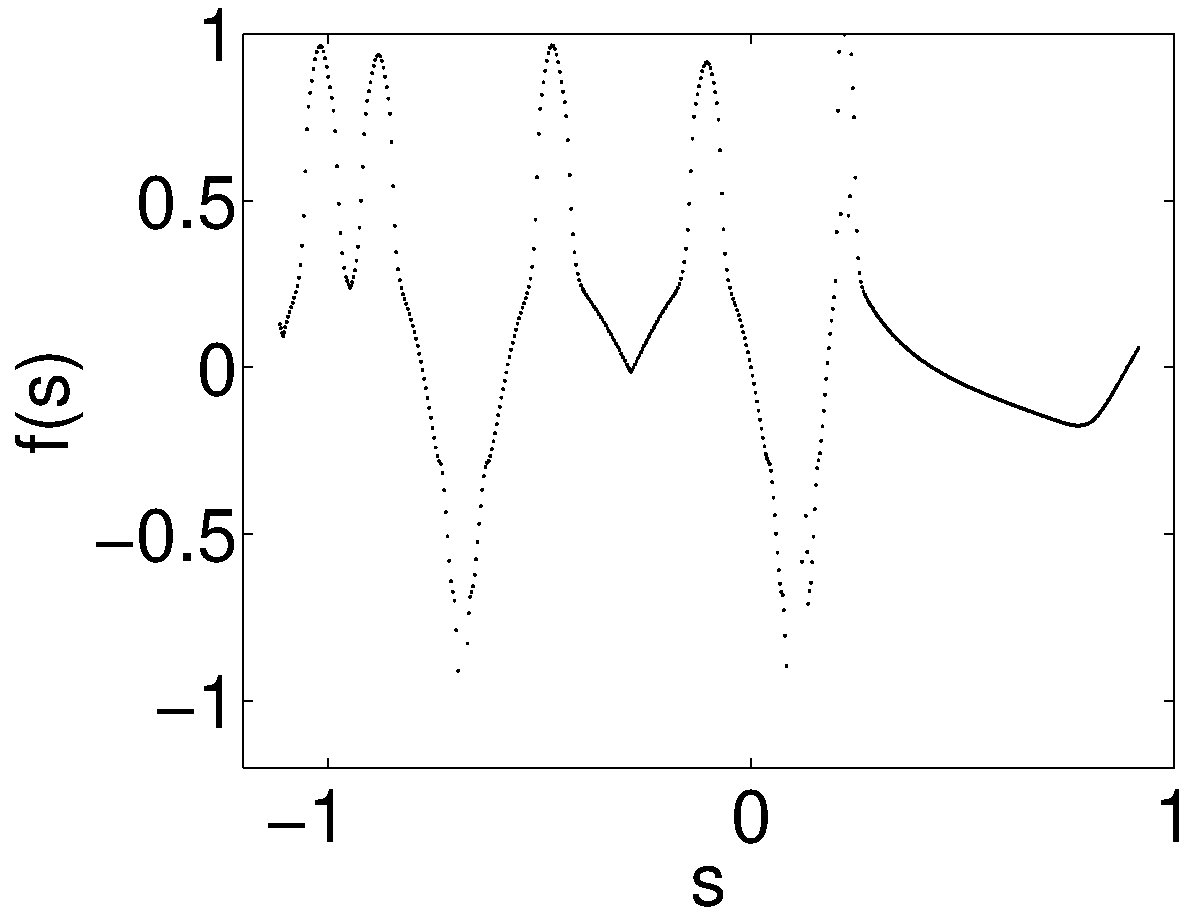
\includegraphics[width=0.74\textwidth]{antmp1}
\\
\hspace{0.10\textwidth}
(a)
\\
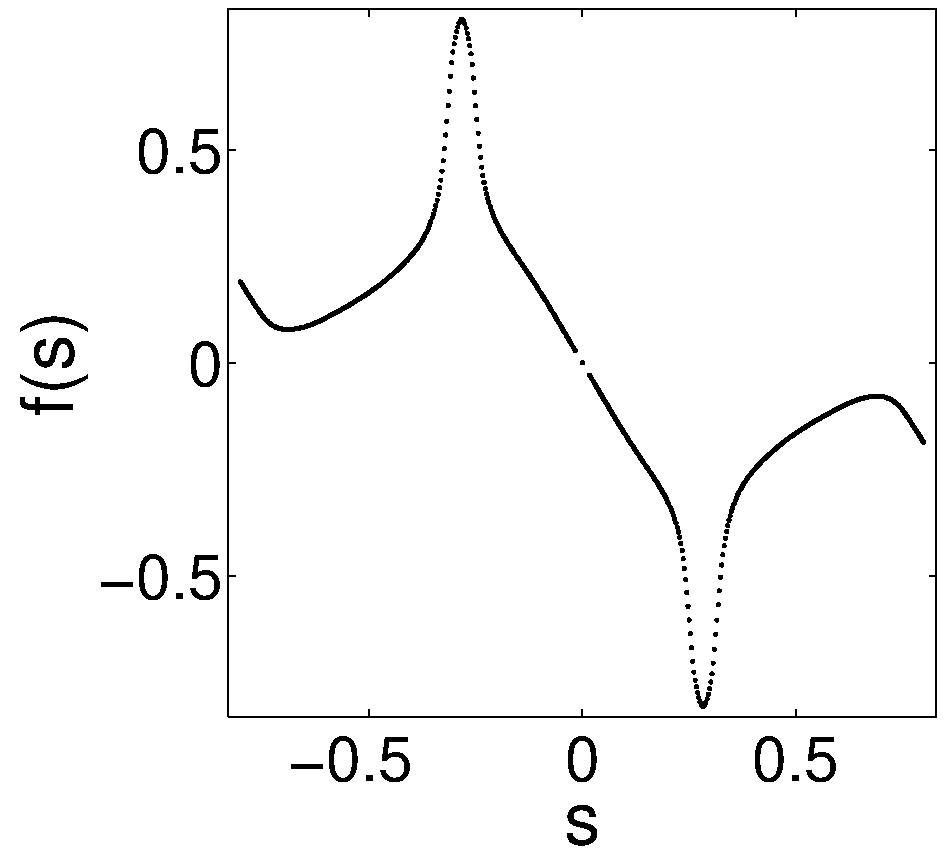
\includegraphics[width=0.44\textwidth]{ant5mmp}
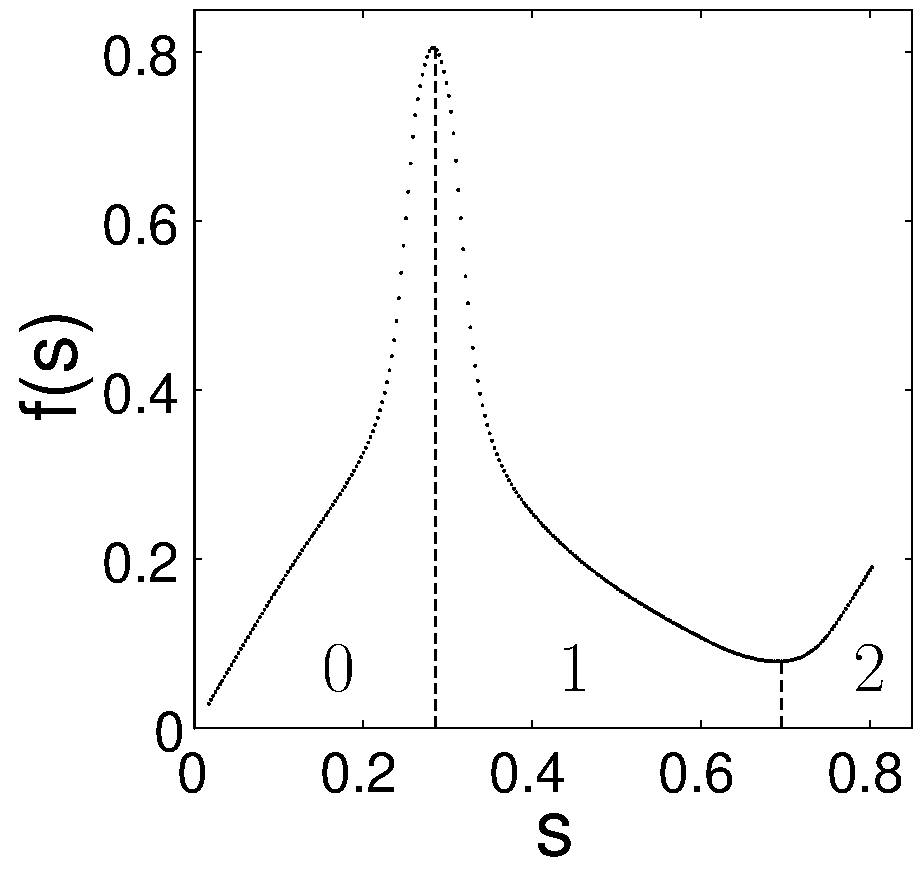
\includegraphics[width=0.44\textwidth]{ant5mmpf}
\\
\hspace{0.10\textwidth}(b)\hspace{0.44\textwidth}(c)
\caption[]{
The \PoincMap\ on the \PoincSec\ $\mathcal{P}_C$ of the
unstable manifold of \eqv\ $C$, antisymmetric subspace of \KS, the
intrinsic coordinate:
(a) There are 11 monotone segments, requiring an 11-letter alphabet.
However, in the (\KS)/{\Dn{1}}-spatial reflection symmetry reduced
\statesp,
(b)
the \PoincMap\ simplifies to an antisymmetric return map,
which becomes
(c)
a 3-letter bimodal return map in the fundamental domain, with the
symbolic dynamics given by three symbols $\{0\,,1\,,2\}$.
It's a \textbf{wild} $\sqrt{\mbox{time}}$ simplification of the dynamics!
enabling us to populate the neighboring strange attractor with
many periodic orbits.
(Taken from fig.~8\,(e) of Lan and Cvitanovi\'c\rf{lanCvit07}).
      }
\label{f:antmn1}
\end{figure}
%%%%%%%%%%%%%%%%%%%%%%%%%%%%%%%%%%%%%%%%%%%%%%%%%%%%%%%%%%%%

    \item[2007-11-20 Keating,  Marklof and Williams]
% doi:10.1088/1367-2630/10/8/083023
The cat map $A$ acting on $(q_\zeit,p_\zeit)$  must be symplectic, and
time-reversal symmetric,
\beq
T A T=A^{-1}
\ee{KeMaWi07(8)}
where $T$ is the time-reversal operator
\beq
T=
\MatrixII{1}{0}
         {0}{-1}
\ee{KeMaWi07(9)}
An example is
% http://shiftleft.com/mirrors/www.hpl.hp.com/techreports/98/HPL-BRIMS-98-07.pdf
% T.O.deCarvalho*,J.P.Keatingi-,J.M.Robbinst
\beq
A=
\MatrixII{2}{1}
         {3}{2}
\ee{CaKero98(9)}
The \PV\ 2-configuration map \refeq{PerViv:2confRepMat}
acts on a 2\dmn\ \statesp\ point $(\ssp_{n-1},\ssp_{n})$,
so time reversal permutes the two entries,
\beq
A=
\MatrixII{0}{1}
         {-1}{s}
\,,\qquad
T=
\MatrixII{0}{1}
         {1}{0}
\,.
\ee{PerViv:2confRepMat1}
Not sure what $T$ is for cat map of form \refeq{eq:CatMapIntr}.


    \item[2004-11-01 Predrag and Lan]
We implemented the ``half-step'' \reffig{fig:HLHalfStepMarkov} reduction
for the \KS\ spatial reflection symmetry in
\HREF{http://chaosbook.org/~predrag/papers/preprints.html\#ks} {\em
Unstable recurrent patterns in Kuramoto-Sivashinsky
dynamics}\rf{lanCvit07}, see \reffig{f:antmn1}.
It happens in sect.~B {\em Curvilinear coordinates, center repeller} of
the paper, and the result is the 3-letter bimodal return map of
\reffig{f:antmn1}\,(c). Without quotienting the $\Dn{1}$ symmetry, the
return map would have up to 11 letters, and be an unmaneagable holly mess.

    \PCpost{2018-04-12}{
For our many (failed) attempts to find an \AW\ forward and
backward in time symmetric partition, see \refsect{sect:timeRev} {\em
Time reversal}.
    }

    \PCpost{2018-04-12}{
\HREF{http://birdtracks.eu/courses/PHYS-7143-19/notes.pdf\#subsection.8.2.3}
{Birdtracks.eu Sect.~8.2.3} {\em  Time reversal symmetry} might be
relevant to \catlatt: when the Hamiltonian is invariant under time
reversal, the symmetry group is enlarged.
    }

    \item[2016-11-16 Predrag]
Maillard group,
Angl{\`e}s d'Auriac, Boukraa and Maillard\rf{AnBoMa99}
{\em Functional relations in lattice statistical mechanics, enumerative
combinatorics, and discrete dynamical systems}
state the ``functional equation''
\beq
\zeta(z)=\zeta(1/z)
\ee{AnBoMa99-3.22a}
which for us is the obvious statement of time-reversal invariance.

    \item[2016-11-16 Predrag]
Note also \refeq{timeRevZeta} under the presumed time reversal $t\to1/t$
%\beq
%\frac{1}{\tilde{\zeta}(1/t)}
%    = -\frac{1}{\tilde{\zeta}(-t)}
%\,.
%\ee{timeRevPC}
This all has to do with time reversibility - we should exploit time and space
reversal symmetries in this way, and - who knows - understand Ihara zeta
functions better.
% It also reminds me of the discrete symmetry factorizations
% of zeta's in ChaosBook.org.

%    \item[2021-01-30 ERROR]
%    Given `square-root' zeta function \refeq{AABHM99-46}
%\beq
%\frac{1}{\tilde{\zeta}(t)}
%    =  \frac{1 - t - t^2}
%            {(1 - t)^2}
%\,,
%\ee{AABHM99-46a}
%$N_n$, the number of \emph{{\lattstate}s} of period $n$ is given by the
%logarithmic derivative of the `square-root' zeta function
%\refeq{zetatop-N},
%\bea
%\sum_{n=1}N_n t^n
%    &=& - \,\frac{1}{\tilde{\zeta}} t \frac{d}{dt} \frac{1}{\tilde{\zeta}}
%\continue
%    &=& -t +  t^2 +2\,t^3 +5\,t^4 +9\,t^5 +16\,t^6 +27\,t^7
%    \ceq
%    +45\,t^8 +74\,t^9 +121\,t^{10} +1971\,t^{11}
%    + \dots
%\,.
%\label{zetasqrt-N}
%\eea


    \item[2020-12-24 Predrag]
Note that in the discussion of time-reversal invariant recurrence
relations \refeq{FGHLW74:charFunct1d} (see \refeq{3diagToeplitz}, \etc)
the characteristic equation factors as $a(\ssp)=\ell(\ssp)\,\ell(l/\ssp)$
where the factors $\ell(\ssp)$ and $\ell(l/\ssp)$ of $a(\ssp)$ are known
as the \emph{Hurwitz factors}.

    \item[2020-01-10 Predrag]
The ``square root'' $C$ \refeq{AABHM99-44} might be related to resistor
networks's Laplace-like operator factorization $L = R\transp{R}$, see
\refeq{Pozrikidis14(1.1.6)}, with no transpose needed in this
example, as $C$ is
symmetric.

%A wild
%$\jMorb=\transp{\tilde{\jMorb}}\tilde{\jMorb}$
%factorization guess, \PCedit{clearly wrong} (works only
%for $s=2$):
%\beq
%\jMorb
%  =
%\left(\begin{array}{ccccccc}
%  {s}&{-1}& 0 & 0 &\dots &0&{-1}\\
%{-1}&   {s}&{-1}& 0 &\dots &0&0 \\
%0 &{-1}&   {s}&{-1}&\dots &0 & 0 \\
%\vdots & \vdots &\vdots & \vdots & \ddots &\vdots &\vdots\\
%0 & 0 & \dots &\dots &\dots  &  {s}&{-1}\\
%{-1}& 0 & \dots &  \dots &\dots&{-1}&   {s}
%        \end{array} \right)
%\,.
%\ee{Pozrikidis14(1.2.10)}
%
%\beq
%\tilde{\jMorb}
%  =
%\left(\begin{array}{ccccccc}
% {1}&{-1}& 0 & 0 &\dots &0& 0\\
% 0 &  {1}&{-1}& 0 &\dots &0&0 \\
% 0 &  0 &  {1}&{-1}&\dots &0 & 0 \\
%\vdots & \vdots &\vdots & \vdots & \ddots &\vdots &\vdots\\
% 0 & 0 & \dots &\dots &\dots  & {1}&{-1}\\
%{-1}& 0 & \dots &  \dots &\dots& 0 &  {1}
%        \end{array} \right)
%\,.
%\ee{Pozrikidis14(1.2.11)}
%
%\beq
%\transp{\tilde{\jMorb}}
%  =
%\left(\begin{array}{ccccccc}
% {1}& 0 & 0 & 0 &\dots &0&{-1}\\
%{-1}&  {1}& 0 & 0 &\dots &0&0 \\
%0 &{-1}&  {1}& 0 &\dots &0 & 0 \\
%\vdots & \vdots &\vdots & \vdots & \ddots &\vdots &\vdots\\
%0 & 0 & \dots &\dots &\dots  & {1}& 0 \\
%0 & 0 & \dots &  \dots &\dots&{-1}&  {1}
%        \end{array} \right)
%\,.
%\ee{Pozrikidis14(1.2.12)}

    \item[2020-02-06 Predrag]
$\jMorb=\transp{\tilde{\jMorb}}\tilde{\jMorb}$ factorization\rf{Pozrikidis14},
% (the $s=3$ or $\mu=1$ guess \refeq{Pozrikidis14(1.2.10)},
% \refeq{Pozrikidis14(1.2.11)} \PCedit{now corrected})
as in
\refeq{sqrtOrbJac}:
\beq
\tilde{\jMorb}
  =
\left(\begin{array}{ccccccc}
 \mu &{-1}  & 0 & 0 &\dots &0& 1\\
 1   &  \mu &{-1}& 0 &\dots &0&0 \\
 0 &  1 &  \mu &{-1}&\dots &0 & 0 \\
\vdots & \vdots &\vdots & \vdots & \ddots &\vdots &\vdots\\
 0 & 0 & \dots &\dots &\dots  & \mu&{-1}\\
{-1}& 0 & \dots &  \dots &\dots& 1 &  \mu
        \end{array} \right)
\,.
\ee{PC(1.2.11)}

\beq
\transp{\tilde{\jMorb}}
  =
\left(\begin{array}{ccccccc}
 \mu& 1 & 0 & 0 &\dots &0&{-1}\\
{-1}&  \mu& 1 & 0 &\dots &0&0 \\
0 &{-1}&  \mu& 1 &\dots &0 & 0 \\
\vdots & \vdots &\vdots & \vdots & \ddots &\vdots &\vdots\\
0 & 0 & \dots &\dots &\dots  & \mu& 1 \\
1 & 0 & \dots &  \dots &\dots&{-1}&  \mu
        \end{array} \right)
\,.
\ee{PC(1.2.12)}
Note that Pozrikidis\rf{Pozrikidis14} $L = R\transp{R}$ factorization
\refeq{Pozrikidis14(1.1.6)} the factors $R$ are bi-diagonal, as in the
forward difference operator \refeq{LatLap}. He does not seem to introduce
1/2 lattice spacing central difference operator \refeq{centeredDiffOper},
and considers only the Helmholtz equation $\mu=0$ case, not our
tri-diagonal map. I do not see our symmetry reduction there...

$\jMorb$ is time reversal \refeq{timeRefl1} invariant (self-adjoint;
Hermitian), $R\jMorb\transp{R}=\jMorb$, but
$\transp{\tilde{\jMorb}}=\tilde{R}\tilde{\jMorb}\transp{\tilde{R}}$ is time reversed, as
a first order derivative should.

%    \item[2020-01-10 Predrag]
%The correct form of $\tilde{\jMorb}$ should agree with the Toeplitz / discrete
%Fourier diagonalization
%\bea
%\lambda_m &=& {\mu}^2+2-2\cos\alpha_m = {\mu}^2+ 4 \sin^2\left(\alpha_m/2\right)
%\continue
%   &=& \left({\mu} - i\,2\sin\left(\frac{\alpha_m}{2}\right)\right)
%   \,  \left({\mu} + i\,2\sin\left(\frac{\alpha_m}{2}\right)\right)
%\continue
%%\,,\quad
%\alpha_m &=& 2\pi{m}/{n}
%\label{Pozrikidis14(1.2.7a)}
%\eea
%\ie, the
%$\sin^2\left(\alpha_m/2\right)$ version of the eigenvalues
%is there for a reason, a consequence of the time-reversal symmetry,
%with $\tilde{\jMorb}$ eigenvalues being
%\[
%-2i\sin\left(\alpha_m/2\right)= \e^{i\alpha_m/2}-\e^{-i\alpha_m/2}
%\,.
%\]
%Phase is $\alpha_m/2$ because the fundamental domain is
%1/2 of the full line.
%The square root is natural because the Yukawa mass ${\mu}^2=d(s-2)$
%parameter \refeq{catlattMass}.

    \item[2020-09-30 Predrag]
Note that in \refeq{AABHM99-46} Maillard \etal\rf{AnBoMa99} quotient the
time reversal (reflection) symmetry for ${s}=3$ \templatt.

The reflection-symmetric operator
\beq
T_{ij} = \sum^d_{\mu=1}
	 [ (\shift^\mu)_{ij} + (\shift^\mu)_{ji}]
	\,,
% \qquad h_\mu = (h,h, \cdots,h)
\label{(5.3)}
\eeq
generates all steps of length 1.
The symmetric (self-adjoint) combination
$\Laplacian = - \transp{\partial}\partial = \partial^2$
 (note this notation for $\Box$)
\index{lattice!Laplacian}\index{Laplacian!lattice}
%(compare with \refeq{(5.3)})
\bea
\Laplacian - {\mu}^2\unit
%\shift^{-1}\partial^2
    &=& - \sum_{\mu=1}^d
\left\{
  \left(\shift^{-1}_\mu  - \unit \right)
  \left(\shift_\mu       - \unit \right)
  + {\mu}^2\unit
\right\}
\continue
\,=\,\jMorb &=&
    \sum_{\mu=1}^d
 \left(\shift^{-1}_\mu + \shift_\mu - {s}\,\unit\right)
\continue
    &=& \left({{T}} -ds \unit\right)
\label{Lat-Lap}
\eea
relates the walker $T$ to the {lattice Laplacian}
and the {\jacobianOrb} $\jMorb$.

    \item[2020-10-31 Predrag]
Han, what does {Gradshteyn and Ryzhik}\rf{GraRyz} have to say about
formulas \refeq{PC:detTemFact}? Sine is a cosine rotated by $\pi/2$.

Still have to factorize the zeta function, as in
\refeq{AABHM99-46}. Clearly
$\det \jMorb_{+}(\mu)=(-1)^\period{}\det \jMorb_{-}(-\mu)$, so,
up to a complex phase, $\det \jMorb_{+}$ is a square root of $\jMorb$.
Not sure anything is attained by computing one rather than the other...


A guess for factorization in
$d$ dimensions (still wrong) is something like
\bea
\Laplacian - d(s-2)\unit
%\shift^{-1}\partial^2
    &=& - \sum_{\mu=1}^d
\left\{
  \left(\shift^{-1}_\mu  - \unit \right)
  \left(\shift_\mu       - \unit \right)
  + (s-2)\unit
\right\}
\continue
    &=& - \sum_{\mu=1}^d
\left\{
-i\left(\shift^{-1}_\mu  - \unit \right)
  + \sqrt{s-2}\,\unit
\right\}
\ceq
\left\{
i\left(\shift_\mu  - \unit \right)
  + \sqrt{s-2}\,\unit
\right\}
\label{Lat-LapGuess}
\eea

    \item[2020-09-30 Predrag]
{\textcolor{red}{Failed attempt, can safely ignore.}}
In $d=1$ \templatt\ case
the time reflection operator $R$, $R^2=\unit$, is
\beq
 {R}  %  = \shift - s\unit + \shift^{-1}
  =
\left(\begin{array}{ccccccc}
 0 & 0 & 0 & 0 &\dots &0& 1 \\
 0 & 0 & 0 & 0 &\dots &1& 0 \\
 0 & 0 & 0 &\dots &1  &0& 0 \\
\vdots & \vdots &\vdots & \vdots & \ddots &\vdots &\vdots\\
 0 & 1 & \dots &\dots &\dots  &0& 0 \\
 1 & 0 & \dots &  \dots &\dots&0& 0
        \end{array} \right)
\,.
\ee{timeRefl1}
with projection operators (for $\cl{}=3$)
\beq
{\PP}_{A_1} = \frac{1}{2}
 \left(\begin{array}{ccc}
 1 & 0 & 1 \\
 0 & 2 & 0 \\
 1 & 0 & 1
  \end{array} \right)
\,,\qquad
{\PP}_{A_2} = \frac{1}{2}
 \left(\begin{array}{ccc}
 1 & 0 &-1 \\
 0 & 0 & 0 \\
-1 & 0 & 1
  \end{array} \right)
\ee{timeP-Aj3}
\beq
{d}_{A_1} = \Tr{\PP}_{A_1} = 2
\,,\qquad
{d}_{A_2} = \Tr{\PP}_{A_2} = 1
\ee{timeP-dim3}
For any $\cl{}$
\beq
{d}_{A_1} = \Tr{\PP}_{A_1} = \frac{1}{2}(\Tr\unit+\Tr R)
          = \frac{1}{2}(\cl{}+1)
\,,\qquad
{d}_{A_2} %= \Tr{\PP}_{A_2}
           = \frac{1}{2}(\cl{}-1)
\ee{timeP-dim-n}
This can only work for $\cl{}$ odd. For even ones there must be another irrep?
\beq
\jMorb_{A_1} = \frac{1}{2}
 \left(\begin{array}{ccc}
 1-{s} & 2     & 1-{s} \\
 2     & -2{s} & 2     \\
 1-{s} & 2     &  1-{s}
  \end{array} \right)
\,,\qquad
\jMorb_{A_2} = \frac{1}{2}
 \left(\begin{array}{ccc}
-1-{s}  & 0 &  1+{s} \\
      0 & 0 &  0 \\
 1+{s}  & 0 & -1-{s}
  \end{array} \right)
\ee{timeOrbJ3}

\beq
\jMorb_{A_1} = \unit +
 \left(\begin{array}{ccc}
 -\frac{1+{s}}{2} & 1 & \frac{1-{s}}{2} \\
 1     & -(1+{s}) & 1     \\
 \frac{1-{s}}{2} & 1     &  -\frac{1+{s}}{2}
  \end{array} \right)
\ee{timeOrbJ3a}

We know that for $[3\!\times\!3]$
{\jacobianOrb}
\bea
\jMorb &=&
\left(
\begin{array}{ccc}
-{s}&  1 &  1 \\
  1 &-{s}&  1 \\
  1 &  1 &-{s}
\end{array}
\right)
    \continue
N_3  &=& |\Det \jMorb|
%   = {s}^3-3{s}-2
    = ({s}-2)({s}+1)^2
    = \left[\mu(\mu^2+3)\right]^2
\,,
\label{catFundPar3}
\eea
but clearly
\beq
\Det\jMorb_{A_1} = 0
\,,\qquad
\Det\jMorb_{A_2} = \frac{1}{4}
 \left(0(1+{s})^2-0(1+{s})^2\right)= {0}
 \,.
\ee{timeDetOrbJ3}
As det of sum is not sum of det's, $\jMorb_{A_1}$, $\jMorb_{A_2}$ are not
fundamental parallelepipeds, and have no geometrical meaning, both have
vanishing determinants. Actually, $\jMorb_{A_1}$ should be invariant
under time reversal, so what did I screw up?
{\textcolor{red}{Failed attempt, done.}}

    \item[2021-03-22 Predrag]
Grava \etal\rf{GKMM21} eq.~\refeq{GKMM21:eq:even_hamiltonian} suggests
what went wrong with the above failed $\Dn{1}$ factorization attempt: we
should have started from the Hamiltonian formulation, decompose the
one-time step temporal evolution [$2\!\times\!2$] {\jacobian} matrix
${\hat{\mathbf{\jMps}}_1}$ that generates a time orbit by acting on the
2\dmn\ `phase space' of successive temporal lattice points
\refeq{PV2configJ} with time reversal ${\bf T}$
\refeq{PerViv:2confRepMat1} decomposing the 2nd order \PV\ time-evolution
equation into two 1st order invariant subspace evolution equations:
\beq
{\bf T}
=\MatrixII{0}{1}
          {1}{0}
\,,\qquad
{\bf \PP}^{+} = \frac{1}{2}
 \MatrixII{1}{1}
          {1}{1}
\,,\;
{\bf \PP}^{-} = \frac{1}{2}
 \MatrixII{1}{-1}
          {-1}{1}
\,.
\ee{PC:HamReversal}
so
\beq
 {\hat{\mathbf{\jMps}}_1}
=
 \left[\begin{array}{cc}
 0 & 1 \\
 -1 & s
 \end{array} \right]
\,;\qquad
 {\hat{\mathbf{\jMps}}_1^{+}}
= \frac{1}{2}
 \left[\begin{array}{cc}
 1   & 1 \\
 s-1 & s-1
 \end{array} \right]
\,,\;
 {\hat{\mathbf{\jMps}}_1^{-}}
= \frac{1}{2}
 \left[\begin{array}{cc}
 -1   & 1 \\
-s-1 & s+1
 \end{array} \right]
\,.
\ee{PC:HamReversal1}
Next: verify the Hill's formula, \refsect{exam:Hill2ndOrd}, and/or
sect.~5. {\em {\HillDet}: stability of an orbit vs. its
time-evolution stability} of {\em siminos/kittens/CL18.tex} for
period-\cl{}\ {\lattstate}s;
\beq
\Det\jMorb_{\pm}
=
\det\left[\unit-({\hat{\mathbf{\jMps}}_1^{\pm}})^\cl{}\right]
\,.
\ee{Hill-Z2factorized}

This establishes, following Fej{\'e}r\rf{Fejer16,RieSzo55} (1916) Fej\'er
and Riesz lemma \refsect{Lemma:FejerRiesz}, -doubting Thomases
non\-with\-standing- that the time reversal invariance leads to
factorization of zeta functions for -hopefully- any temporal lattice
systems with time-inversion $\zeit \to -\zeit$ invariance.

As far as I can tell, we are the first to make this claim for
time evolution, not for spatially discrete or $N$-body systems.

Sidney and Han, please go to \refsect{sect:pw2021-03-22}~{\em Pow wow
2021-03-22} and do the homework. Call me any time for any clarifications
you need. As always, everything prof says might be wrong, so remain
vigilant. And stay safe.

    \item[2021-03-22 Predrag]
    {\textcolor{red}{The above might be a failed attempt again...}}, as
\PV\ form is not right: $[{\bf T},{\mathbf{\jMps}}_1]\neq0$:
\beq
{\bf T}
=\MatrixII{0}{1}
          {1}{0}
\,,\qquad
{\bf \PP}^{+} = \frac{1}{2}
 \MatrixII{1}{1}
          {1}{1}
\,,\;
{\bf \PP}^{-} = \frac{1}{2}
 \MatrixII{1}{-1}
          {-1}{1}
\,.
\ee{PC:HamReversalPV}
so
\beq
 {\hat{\mathbf{\jMps}}_1}
=
 \left[\begin{array}{cc}
 0 & 1 \\
 -1 & s
 \end{array} \right]
\,;\qquad
 {\hat{\mathbf{\jMps}}_1^{+}}
= \frac{1}{2}
 \left[\begin{array}{cc}
 1   & 1 \\
 s-1 & s-1
 \end{array} \right]
\,,\;
 {\hat{\mathbf{\jMps}}_1^{-}}
= \frac{1}{2}
 \left[\begin{array}{cc}
 -1   & 1 \\
-s-1 & s+1
 \end{array} \right]
\,.
\ee{PC:HamReversal1PV}


    \item[2020-11-18 Predrag]
Factorization \refeq{AxFlNi16(2.7)}
\beq
A=
\MatrixII{2}{1}
         {1}{1}
=
\MatrixII{1}{1}
         {0}{1}
\MatrixII{1}{0}
         {1}{1}
% = LR^{-1}
= L\transp{L}
%\,,
% \qquad\det A= 1 \,,
\ee{AxFlNi16(2.7)PC}
leads to
\beq
\det(1-t\transp{L})\,\det(1+tL)
    =  {\det(1-zA)}
\ee{AABHM99-56ePC}
which also verifies \refeq{AABHM99-46}. Both \refeq{prArnoldCat},
\refeq{AxFlNi16(2.7)} are symmetric under transposition. What about the
asymmetric \PV\ \refeq{PerViv:2confRepMat}? The similarity transformation
\refeq{HLsimilarityC} that maps \refeq{ArnoldCat} into
\refeq{PerViv:2confRepMat},
\beq
{\bf A}
=\MatrixII{2}{1}
          {1}{1}
\,,\qquad
{\bf B}
=\MatrixII{0}{1}
          {-1}{3}
\,,
\ee{HLsimilarityB1}
is
\beq
{\bf B} = {\bf S}^{-1}{\bf A}{\bf S}
\,,
\ee{HLsimilarityC1}
where
\[
{\bf S} = {\bf S}^{-1}
        =\MatrixII{-1}{2}
				   {0}{1}
\,.
\]
See also discussion around \refeq{AABHM99-44HL} and \refeq{sim2PV}.

    \item[2021-02-10 Predrag] I looked cursorily at it
and did not spot anything, but it is of possible interest:

Terry Loring and Fredy Vides
% https://dx.doi.org/10.1063/5.0023028
{\em Computing Floquet Hamiltonians with Symmetries}
\arXiv{2007.06112}

    \item[2021-04-10 Predrag]
For specializing  \refexam{exam:StandMapSymmLin}~{\em Symmetry lines of the standard map}
to cat map, see \refexam{exam:CatMapSymmLin}~{\em Symmetry lines of the cat map}.

    \item[2021-04-10 Predrag]
For a scholarly discussion of many facets of ``time-reversal'', see the
essay \HREF{http://philsci-archive.pitt.edu/15033/}
{{\em Time Reversal}} by Bryan W. Roberts (2019).

    \item[2021-04-14 Predrag to Stephen]
In spirit of our `square root' philosophy,
\HREF{https://writings.stephenwolfram.com/2021/04/the-wolfram-physics-project-a-one-year-update/}
{Wolfram Physics Project} writes:
 \begin{quote}
Another promising possibility relates to the distinction between fermions
and bosons. We’re not sure yet, but it seems as if Fermi–Dirac statistics
may be associated with multiway graphs where we see only non-merging
branches, while Bose–Einstein statistics may be associated with ones
where we see all branches merging. Spinors may then turn out to be as
straightforward as being associated with directed rather than undirected
spatial hypergraphs.
 \end{quote}
The problem is that I cannot find a technical paper on that,
if it exists. I do not find any hint of this in his
Wolfram\rf{Wolfram20}
{\em A Project to Find the Fundamental Theory of Physics}.

That jives with our spatiotemporal cat work. There the graph is just a
d-dimensional undirected hypercubic lattice,  but reflection symmetry
reduces the graph to a pair of directed graphs, much like reducing the
Klein-Gordon Laplacian to two Dirac operators.

    \item[2021-04-15 Stephen]
There's nothing yet on our home pages.

Very interesting!   Now I just went searching in your material ... and
couldn't find this either.  Can you point me to this?

I'm wondering if it's at all related to the (disappointingly vague)
\HREF{https://www.wolframscience.com/nks/notes-9-16--discrete-quantum-mechanics/}
{notes-9-16--discrete-quantum-mechanics}.
({\bf 2021-04-16 Predrag}: Read this, do not see any connection to our work.)

I saw various Klein-Gordan-like equations in your works ... but nothing
Dirac like (did I miss it?)

The d-dimensional hypercubic lattice obviously has certain discrete
symmetry.  Does the ``square root lattice'' have some other identifiable,
and perhaps spinorial, symmetry?

By the way ... if you're up for it sometime, I'd love to try to talk
through the
geodesic-balls-in-hypergraphs-have-limiting-symmetries-that-are-Lie-groups
story.  Your hypercubic lattice is too ``special'' ... but imagine a random
d-dimensional lattice (for integer d).  Then presumably the invariances
of the geodesic ball limit to \SOn{d}.  But what happens with one-way vs
two-way connections?  How does it affect representations?  What about
fractional d?  Etc. etc.    I have a suspicion that with your help this
might be able to be cracked...


    \item[2021-04-17 Predrag to Tony Kennedy] <Tony.Kennedy@ed.ac.uk>

You might be The Man for the job:

We are stuck on reflection-symmetry reduction needed to factorize the
zeta functions. Here is a simple way to explain what the problem is:

Think of a discrete time dynamical system (iterations of a map) as a
1-dimensional lattice with the field on each site labeled by integer
time. An period-$\cl{}$ {\lattstate} lives on a discrete 1-torus (a ring or
necklace) of period $n$, and if the law is time-independent, sets of
solutions are invariant under cyclic perturbations. The symmetry is
\Cn{n}, and one needs to distinguish \Cn{n} orbits
(''{prime cycle}s'' in ChaosBook; one per each orbit).
The right way to do this is by going to
\Cn{n} irreps, ie, by the discrete Fourier transform, with all reciprocal
lattice Brillioun zone solutions {\orbit}s in an $1/n$ sliver of a
$n$-gon. If $n$ is prime, this is irreducible; if it is a multiple of a
prime, one should remove those solutions, as they have already been
accounted for.

If, in addition, the law is time-reversal (or time-inversion) invariant,
the symmetry includes time-reflection, ie, it is dihedral group \Dn{n}
with 2$n$ elements, so the reciprocal lattice should be a half of the
above 1/$n$ sliver of a $n$-gon, and irreps are now either 1 or 2
dimensional. Even $n$ is different from odd $n$, and solutions either appear
in pairs, or are self dual under reflection in 3 different ways.

ChaosBook works out zeta function factorizations for \Dn{1},
\Dn{2}
(known as \HREF{https://groupprops.subwiki.org/wiki/Klein_four-group}{Klein four-group}),
\Dn{3} (symmetric group $S_3$), and \Dn{4}, but somehow I get confused by all the
invariant subspaces of solutions for \Dn{n},  so we are stuck... Not to
mention counting orbits for a Bravais lattices (doubly periodic {\lattstate}s) for \catlatt. There we do not know how to write down the zeta
function, let alone factorize it into irreps of the discrete symmetry
group of a given Bravais lattice.

For more detail, see
\refsect{s:latt1d} {\em Dihedral groups}.

    \item[2021-05-04 Predrag]
Can one write the {\jacobianOrb} of a repeat of a $p$-cycle as
a product of $p$-cycle {\jacobianOrbs}?\\
({\bf 2021-06-14 Predrag}
{\color{green}This is now accomplished} by the block matrix
formulation \refeq{JacOrbitRepeated}.)
\bea
\jMorb_p^{(2)}\jMorb_p^{(1)}
 &=&
\begin{bmatrix}
1 & 0 & 0 & 0 & 0 & 0\\
0 & 1 & 0 & 0 & 0 & 0\\
0 & 0 & 1 & 0 & 0 & 0\\
0 & 0 & 0 & \field_0 & 1        & 1 \\
0 & 0 & 0 & 1        & \field_1 & 1\\
0 & 0 & 0 & 1        & 1        & \field_2
\end{bmatrix}
\begin{bmatrix}
\field_0 & 1 & 1 & 0 & 0 & 0\\
1 & \field_1 & 1 & 0 & 0 & 0\\
1 & 1 & \field_2 & 0 & 0 & 0\\
0 & 0 & 0        & 1 & 0 & 0\\
0 & 0 & 0        & 0 & 1 & 0\\
0 & 0 & 0        & 0 & 0 & 1\\
\end{bmatrix}
    \continue
 &\neq&
\begin{bmatrix}
\field_0 & 1 & 0 & 0 & 0 & 1\\
1 & \field_1 & 1 & 0 & 0 & 0\\
0 & 1 & \field_2 & 1 & 0 & 0\\
0 & 0 & 1 & \field_0 & 1        & 0 \\
0 & 0 & 0 & 1        & \field_1 & 1\\
1 & 0 & 0 & 0        & 1        & \field_2
\end{bmatrix}
\,,
\label{notRepeatOrbitJac}
\eea
Another try:
\bea
\jMorb_p^{(2)}\jMorb_p^{(1)}
 &=&
\begin{bmatrix}
1 & 0 & 0 & 0        & 0        & 1\\
0 & 1 & 0 & 0        & 0        & 0\\
0 & 0 & 1 & 1        & 0        & 0\\
0 & 0 & 1 & \field_0 & 1        & 0 \\
0 & 0 & 0 & 1        & \field_1 & 1\\
1 & 0 & 0 & 0        & 1        & \field_2
\end{bmatrix}
\begin{bmatrix}
\field_0 & 1        & 0        & 0 & 0 & 1\\
1        & \field_1 & 1        & 0 & 0 & 0\\
0        & 1        & \field_2 & 1 & 0 & 0\\
0        & 0        & 1        & 1 & 0 & 0\\
0        & 0        & 0        & 0 & 1 & 0\\
1        & 0        & 0        & 0 & 0 & 1\\
\end{bmatrix}
    \continue
 &\neq&
\begin{bmatrix}
\field_0+1 & 1 & 0 & 0 & 0 & 2\\
1 & \field_1 & 1 & 0 & 0 & 0\\
0 & 1 & \field_2+1 & 2 & 0 & 0\\
0 & 0 & 1 & \field_0+1 & 1        & 0 \\
0 & 0 & 0 & 1        & \field_1 & 1\\
\field_0+\field_2 & 0 & 0 & 0        & 1        & \field_2+1
\end{bmatrix}
\,,
\label{notRepeatOrbitJac1}
\eea
(partly wrong, but does not matter), so
{\jacobianOrbs} do not multiply.

But they do not add up, either, cannot reconcile the small block periodic
\bcs\ with the repeated block \bcs. Defeated again.


\end{description}



\subsection{Poles of dynamical zeta functions}
\begin{description}
    \item[1993-03-11 Predrag]
A clip from (boyscouts only)
ChaosBook Chapter~{\em Quantum pinball},
% based on Predrag        25feb2002 Phys Rev Lett with Eckhardt
% {\em Resonances of a chaotic scatterer}, \texttt{eck\_letter1.tex}.
taken from Predrag's \texttt{c.tex}\rf{CERRS},
Casati and Shilnikov\rf{GiBo}.

    \item[2020-11-07 Predrag] In 1993 I have not thought of
\refeq{CERRS(1.87a)} as clue to time-reversal factorization, but
the Hamiltonian weight, one per each degree of freedom,
\beq
\det ({\bf 1}-{\bf J}_p)
  = (1-\Lambda_p)(1-1/\Lambda_p)
  = - \Lambda_p +2 -1/\Lambda_p
\ee{CERRS(1.87aa)}
sure looks suggestive, in the spirit of
\refeq{HLmatrix}. It leads to factorization
\refeq{qP:doub_pole},
\beq
1/\zeta_j = \frac{F_j}{F_{j+1}}\,\frac{F_{j+2}}{F_{j+1}}
\,\, ,
\label{qP:doub_polePC}
\eeq
compare with \refeq{AABHM99-46}.



\end{description}

For a Hamiltonian two degree of freedom system, ${\bf J}_p$ is a
[$2\times2$] matrix with
unit determinant. If the cycle is unstable, the eigenvalues
$\Lambda_p$ and $1/\Lambda_p$ are real, and we
denote the expanding eigenvalue by $\Lambda_p$.
The denominator can then be expanded in a
geometric series
\beq
    1/ |\det ({\bf J}_p-{\bf 1})| = |\Lambda_p|^{-1} (1-1/\Lambda_p)^{-2} =
     |\Lambda_p|^{-1} \sum_{j=0}^\infty (j+1) \Lambda_p^{-j} \, .
\ee{CERRS(1.87a)}
Performing the $r$ summation and interchanging
sums and logarithms one ends up with
%% \beq
$     \Omega(s) = {\partial \over \partial s} \ln F(s) $,
%% \eeq
where $F(s)$ is the {\em classical Fredholm determinant }
\beq
     F(s) = \prod_{p} \prod_{j=0}^\infty
     \left( {1- |\Lambda_p|^{-1} \Lambda_p^{-j}  e^{s T_p}} \right)^{j+1}
      \, .
\label{F_class}
\eeq
As $\Omega(s)$ is a logarithmic derivative, its poles are
given by the zeros and poles of $F(s)$.
Denoting the classical weight of the cycle $p$ by
\beq
        t_p = z^{n_p} e^{s T_p}/ {|\Lambda_p|}
\label{t_p_class}
\eeq
and defining {\em dynamical zeta functions}~\cite{ruelle}
\beq
1/\zeta_j
         = \exp\left( - \sum_p \sum_{r=1}^\infty \frac{1}{r}
                      ({t_p / {\Lambda_p^j}})^r \right)
         =  \prod_p  \left( 1 -{ t_p / {\Lambda_p^j}}  \right)
\,\, ,
\label{zeta_j}
\eeq
the Fredholm determinant (\ref{F_class})
can be written as an infinite product over $1/\zeta_j$:
\beq
     F(s) =
        \prod_p\prod_{j=0}^{\infty} (1-t_p/\Lambda_p^{j})^{j+1}
        =\prod_{j=0}^{\infty} 1/\zeta_j^{j+1}
\,\, .
        % \prod_{j=0}^\infty 1/\zeta_j^{j+1} \, .
\label{fredholm}
\eeq
We have introduced a bookkeeping variable $z$
raised to the power of the topological length (number of disk
collisions in a cycle) in order to be able to systematically
expand the infinite products in terms of increasing
topological cycle length.


The double pole is not as surprising
as it might seem at the first glance; indeed,
the theorem that establishes that
the classical Fredholm determinant (\ref{fredholm})
is entire implies that the
poles in $1/\zeta_j$ must have right multiplicities in order
that they be cancelled in the $ F = \prod 1/\zeta_j$ product. %~\cite{CR92}.
More explicitly, $1/\zeta_j$ can be expressed in terms of
weighted Fredholm determinants
\beq
F_j =
    \exp\left( - \sum_p \sum_{r=1}^\infty \frac{1}{r}
                 { {({t_p / {\ExpaEig_p^j}})^r}
                  \over
                   {(1-1/\ExpaEig^r_p)^2}
                 }
        \right)
\label{F_j}
\eeq
by inserting the identity
\beq
1= {1 \over {(1-1/\ExpaEig)^2}}
   -{2\over \ExpaEig} {1 \over {(1-1/\ExpaEig)^2}}
   + {1 \over {\ExpaEig^2}} {1 \over {(1-1/\ExpaEig)^2}}
\ee{qP:Lapl}
into the exponential representation (\ref{zeta_j})
of $1/\zeta_j$.
This yields
\beq
1/\zeta_j = { {F_j F_{j+2}} \over {F_{j+1}^2}}
\,\, ,
\label{qP:doub_pole}
\eeq
and we conclude that for 2-dimensional Hamiltonian flows the
dynamical zeta function $1/\zeta_j$ has a {\em double} leading pole
coinciding with the leading zero of the $F_{j+1}$
Fredholm determinant.



\renewcommand{\ssp}{x}
\renewcommand{\Ssym}[1]{{\ensuremath{s_{#1}}}}    % Boris
\renewcommand{\Xx}{\ensuremath{\mathsf{X}}}      % Boris

\newpage %TEMP
% siminos/spatiotemp/chapter/reversLit.tex
% $Author: predrag $ $Date: 2021-12-22 18:29:33 -0500 (Wed, 22 Dec 2021) $

\section{Time reversal literature}
\label{sect:reverLit}
\renewcommand{\ssp}{\ensuremath{\phi}}             % lattice site field
\renewcommand{\Ssym}[1]{{\ensuremath{m_{#1}}}}    % Boris
\renewcommand{\Xx}{\ensuremath{\mathsf{\Phi}}}      % kittens lattice field

%\newpage
\subsection{Grava \etal\ 2021 paper {GKMM21}}
\label{sect:GKMM21}
% [2021-03-20 Predrag]
Notes on
Grava, Kriecherbauer,  Mazzuca and McLaughlin\rf{GKMM21}
{\em Correlation functions for a chain of short range oscillators},
\arXiv{2010.09612}:
\bigskip

[C]onsider a system of $N=2M+1$ particles interacting with a short range
harmonic potential with 	 Hamiltonian of the form
	\begin{equation}
	\label{GKMM21:H0}
H=\sum_{j=0}^{N-1}\frac{p_j^2}{2}+\sum_{s=1}^m\frac{\kappa_s}{2}\sum_{j=0}^{N-1}(q_j-q_{j+s})^2\,,
\end{equation}
and
Hamiltonian density
\[
e_j=\frac{p_j^2}{2}+\frac{1}{2} \Big(\sum_{s=1}^m \tau_s (q_{j+s}-q_j)
\Big)^2
\,,
\]
local in the variables $({\bf{p}},{\bf{q}})$ for fixed $m$.  If we let
$N\to\infty$, the quantity $e_j$ involves a finite number of physical
variables  $({\bf{p}},{\bf{q}})$.
We always take periodic boundary conditions,
the indices $j$ are taken from $\integers / N\integers$ and therefore
\[
q_{N+j}=q_j,\quad p_{N+j}=p_j
\]
holds for all $j$.

The relative shift \tilt{}  boundary condition $q_{N+1}=q_1+\tilt{}$ can
be also be considered  (see e.g.~\refref{Spohn14}). The periodic boundary
condition is recovered by  change  of coordinates $q_j\to
q_j-\frac{\tilt{}}{N}(j-1)$.

The coefficients $\tau_s$ are the entries of the circulant localized
square root $T$ of the matrix  $A$ by which we mean a solution of the
equation \refeq{GKMM21:eq:T0} of the form \refeq{GKMM21:form:T}.

The  Hamiltonian \refeq{GKMM21:H0} can be rewritten in the form
			\begin{equation}
	\label{GKMM21:eq:A}
	H({\bf{p}},{\bf{q}}) := \frac{1}{2} \langle{\bf{p}}, {\bf{p}}\rangle +\frac{1}{2}\langle {\bf{q}},A {\bf{q}}\rangle,
	\end{equation}
	where ${\bf{p}}=(p_0,\dots,p_{N-1}) $, ${\bf{q}}=(q_0,\dots,q_{N-1}),$  $\langle\,.,\,.\rangle$ denotes the standard scalar product in $\R^N$ and
	where $A\in\mbox{Mat}(N,\R)$ is a positive semidefinite  symmetric   circulant matrix generated by the vector  ${\bf{a}}=(a_0,\dots,a_{N-1})$ namely $A_{kj}=a_{(j-k)\mbox{\tiny {mod $N$}}}$ or
	\begin{equation}
	\label{GKMM21:A}
			A = {\begin{bmatrix}
				a_{0}&  a_{1}&\dots & a_{N-2}& a_{N-1}
				\\
				a_{N-1}& a_{0}& a_{1}&& a_{N-2}
				\\
				\vdots & a_{N-1}& a_{0}&\ddots &\vdots
				\\
				a_{2}&&\ddots &\ddots & a_{1}
				\\
				a_{1}& a_{2}&\dots & a_{N-1}& a_{0}
				\\
				\end{bmatrix}}\, ,
		\end{equation}
The harmonic oscillator with  only  nearest neighbour interactions  is recovered by choosing
\[
a_0=2\kappa_1,\quad a_1=a_{N-1}=-\kappa_1,
\]
and the remaining coefficients  are set to zero.

The equations of motion  for the Hamiltonian $H$  take the form
\beq
\dfrac{d^2}{dt^2}q_j=\sum_{s=1}^m \kappa_s (q_{j+s}-2q_j+q_{j-s}),\quad j\in\integers / N\integers.
\ee{GKMM21:Lagr}
{
The integration is obtained  by studying the dynamics in Fourier space.
%  (see e.g. \cite{Lukkarinen}).
[...]
Following the standard procedure in the case of
nearest neighbour interactions we replace the vector of position ${\bf{q}}$ by
a new variable ${\bf{r}}$ so that the Hamiltonian takes the form
 \[
H=\frac{1}{2}\langle {\bf{p}},{\bf{p}}\rangle+\frac{1}{2}\langle{\bf{r}},{\bf{r}}\rangle.
\]
Such a change of variables may be achieved by any linear transformation
\begin{equation}
\label{GKMM21:r}
{\bf{r}}=T{\bf{q}},
\end{equation}
with an $N\times N$ matrix $T$ that satisfies
\begin{equation}
	\label{GKMM21:eq:T0}
		A = T^\intercal T,
	\end{equation}
where $ T^\intercal$ denotes the transpose of $T$.

In the case of nearest neighbour interactions one may choose
\[
r_j = \sqrt{\kappa_1} (q_{j+1}-q_j)
\]
corresponding to a circulant matrix $T$
generated by the vector
\[
\boldsymbol{\tau}=\sqrt{\kappa_1}(-1,1,0,\dots,0)
\,.
\]
We show that short range interactions given by matrices $A$ of the
form~\refeq{GKMM21:A} also admit such a {\em localized square root}. More
precisely, there exists a circulant $N\times N$ matrix $T$ of the form
\beq\label{GKMM21:form:T}
			T ={\begin{bmatrix}
				\tau_0&  \tau_{1}&\dots&  \tau_{m}&0 &\dots&0	\\			
				0& \tau_{0}& \tau_{1}&\dots&\tau_m&0&				\\
				&\ddots & \ddots& \ddots &\ddots &&\\
%				&&&&&&&&&\\
%	&&&&&&&&&\\
%	&&&&&&&&&\\
%	&&&&&&&&&\\
%	&&&&&&&&&\\
                                 \tau_m&0&\ddots & \ddots& \ddots &\ddots &\\
                                 				&\ddots & \ddots& \ddots &\ddots & \ddots&\ddots\\
				\tau_2&\dots&\tau_m&0&\dots&\tau_0&\tau_1\\
				\tau_1&\tau_2&\dots&\tau_m &0&0&\tau_{0}
				\\
				\end{bmatrix}}
\,.
\eeq
that satisfies \refeq{GKMM21:eq:T0}. The crucial point here is that $T$ is not the standard (symmetric) square root of the positive semidefinite matrix $A$ but a localized version generated by some vector $\boldsymbol{\tau}$
with zero entries everywhere, except possibly in the first $m+1$ components.
[...]
Note that $\boldsymbol{1}=(1,\ldots, 1)^\intercal$ satisfies $T \boldsymbol{1}=0$ since $\langle \boldsymbol{1}, A\boldsymbol{1}\rangle =0$. This implies
$$\sum_{s=0}^m\tau_s=0\,, \quad
r_j= \sum_{s=1}^{m} \tau_s (q_{j+s}-q_j)\,  \quad \text{and} \quad \sum_{j=0}^{N-1}r_j= (1,\ldots, 1) T {\bf{q}} = 0.$$
The local energy $e_j$ takes the form
\[
e_j=\dfrac{1}{2}p_j^2+\dfrac{1}{2}r_j^2\,.
\]
Due to the spatial translation invariance of the Hamiltonian
\[
H({\bf{p}},{\bf{q}}) = H({\bf{p}},{\bf{q}}+\lambda \boldsymbol{1})
\,,
\] $\lambda \in \R$,
that corresponds to the conservation of total momentum, we reduce the
Hamiltonian system by one degree of freedom, with the reduced phase space
		\begin{equation}
	\label{GKMM21:eq:phase_space}
	{\mathcal M}
:=
\left\{({\bf{p}},{\bf{q}})\in \R^{N}\times \R^{N}
\, : \, \sum_{k=0}^{N-1} p_k =0\, ;\, \sum_{k=0}^{N-1} q_k = 0 \right\}
\,.
	\end{equation}

[...]
the dispersion relation  $|\omega(k)|$  for the harmonic oscillator with
short range interaction in the limit $N\to\infty$ obtaining
\beq
	\label{GKMM21:dispersion0}
	f(k)=|\omega(k)|
=\sqrt{2\sum_{\ell=1}^m\kappa_\ell\left(1-\cos(2\pi k\ell)\right)}
\,,
\eeq
[...]
we show that the evolution equations for the generalized position,
momentum can be written in the form of  conservation laws which have a
potential function.
 For the case of the harmonic oscillator with nearest neighbour interaction, we show that this function is  a Gaussian random variable
and determine the leading order behaviour of its variance as $t\to\infty$.

[...] some notation.   First of all,  a matrix $A$ of the form
\refeq{GKMM21:A} with ${\bf{a}}\in\R^N$ is called a circulant matrix generated by the vector ${\bf{a}}$.
	\paragraph{$m$-physical vector and half-$m$-physical vector}
	\label{GKMM21:def:ph}
			Fix $m \in {\mathbb N}$.
			For any odd $ N > 2m$, a   vector $\tilde{\bx}\in \R^{N}$  is said to be  {\em $m$-physical} generated by $\bx=(x_0,x_1,\dots, x_m)\in \R^{m +1}$ if $x_0=-2\sum_{s=1}^mx_s$ and 				
			\begin{align}
            \label{GKMM21:HalfVector}
				\tilde{x}_0 = & x_0 \, ,\\
				\tilde{x}_1= &\tilde{x}_{N-1} = x_1<0 ,\;\;\tilde{x}_m= \tilde{x}_{N-m} = x_m<0,\\
			\tilde{x}_k= &\tilde{x}_{N-k} = x_k \leq 0, \mbox{ for  $1< k <  m$},\\
			 \tilde{x}_{k} =& 0, \mbox{  otherwise,}
						\end{align}
	while the  vector  $\tilde{\bx}\in \R^{N}$  is called  {\em half-$m$-physical} generated by ${\bf{y}}\in  \R^{m +1}$ if  $y_0=-\sum_{s=1}^my_s$  and	\begin{align*}
		\tilde{x}_k=  & y_k,  \mbox{ for  $0 \leq k \leq m$   } \\
		\tilde{x}_k=&0,  \mbox{ for  $m< k \leq N-1$.   }
		\end{align*}
Following  the proof of a lemma by Fej\'er and Riesz, one can show that a
circulant symmetric matrix $A$ of the form \refeq{GKMM21:eq:A}  generated
by  a $m$-physical vector ${\bf{a}}$ always has a circulant localized
square root
%{\em Golub - Toepliz} \cite{Golubov}, the next proposition shows that
% a circulant symmetric matrix $A$ of the form \refeq{GKMM21:eq:A}  generated by
% a $m$-\th{physical} vector ${\bf{a}}$ always has a circulant localized square root
$T$  that is generated by a half-$m$ physical vector ${\boldsymbol{\tau}}$.

\paragraph{Fej\'er and Riesz~\cite[pg.~117 f]{RieSzo55} lemma}
\label{Lemma:FejerRiesz}
asserts that every positive
trigonometric polynomial can be represented by the square of the absolute
value of another trigonometric polynomial whose coefficients are, in
general, complex.
\bigskip

Fix $m \in {\mathbb N}$. Let the circulant matrix $A$ be generated by an
$m$-physical vector ${\bf{a}}$, then there exist a circulant matrix $T$
generated by an half-$m$-physical vector ${\boldsymbol{\tau}}$ such that:
	\begin{equation}
	\label{GKMM21:eq:T}
		A = T^\intercal T\,.
	\end{equation}
Moreover, we can choose ${\boldsymbol{\tau}}$ such that $\sum_{s=1}^m s
\tau_s > 0$. Then one has $\sum_{s=1}^m s
\tau_s=\sqrt{\sum_{s=1}^ms^2\kappa_s}$.

For  example,  if  we consider $m=1$, and $a_0=2\kappa_1$ and
$a_1=a_{N-1}=-\kappa_1$.  The matrix $T$ is generated by the vector
${\boldsymbol{\tau}}=(\tau_0,\tau_1)$ with $\tau_0=-\sqrt{\kappa_1}$ and
$\tau_1= \sqrt{\kappa_1}$.
When $m=2$ and  $a_0=2\kappa_1+2\kappa_2$,  $a_1=a_{N-1}=-\kappa_1$,  $a_2=a_{N-2}=-\kappa_2$. The matrix $T$ is generated by the vector ${\boldsymbol{\tau}}=(\tau_0,\tau_1,\tau_2)$
with
\begin{align*}
&\tau_0=- \frac{\sqrt{\kappa_1}}{2}-\frac{1}{2}\sqrt{\kappa_1+4\kappa_2}, \;\;\tau_1=\sqrt{\kappa_1},\\
&\tau_2=-\frac{\sqrt{\kappa_1}}{2}+\frac{1}{2}\sqrt{\kappa_1+4\kappa_2},\end{align*}
so that the quantities $r_j$ are defined as
\[
r_j=\tau_1(q_{j+1}-q_j)+\tau_2 (q_{j+2}-q_j)\,,\quad j\in\integers / N\integers \,.
\]
[...]
The Hamiltonian $H({\bf{p}},{\bf{q}})$	represents clearly an integrable system  that can be integrated passing through Fourier transform.
Let ${\mathcal F}$ be the discrete Fourier transform with entries  ${\mathcal F}_{j,k}:=
\frac{1}{\sqrt{N}} e^{- 2\im \pi j k/N}$ with $j,k=0,\dots, N-1$. It is immediate to verify that
	\begin{equation}
	\label{GKMM21:DHT_prop}
	{\mathcal F}^{-1} = \bar{{\mathcal F}} \qquad {\mathcal F}^\intercal = {\mathcal F}.
	\end{equation}
	Thanks to the above  properties,  the transformation defined by
	\begin{equation}
	\label{GKMM21:eq:F_variables}
	(\hat{\bf{p}}, \hat{\bf{q}}) = (\bar{\mathcal F} p, {\mathcal F} q)
	\end{equation}
	is canonical.  Furthermore
$\bar{\hat{\bf{p}}}_j = \hat{\bf{p}}_{N-j}$  and $\bar{\hat{\bf{q}}}_j = \hat{\bf{q}}_{N-j}$,
for $j=1,\dots,N-1$, while  $\hat{\bf{p}}_0$ and  $\hat{\bf{q}}_0$ are real variables.
The matrices  $T$ and $A$ are  circulant matrices and so they are reduced to diagonal form by
${\mathcal F}$:
\[
{\mathcal F} A {\mathcal F}^{-1}
= {\mathcal F} T^\intercal T{\mathcal F}^{-1}
=\overline{({\mathcal F} T{\mathcal F}^{-1})}^\intercal ({\mathcal F} T{\mathcal F}^{-1})
\;.
\]
Let  $\omega_j$ denote the eigenvalues of the matrix $T$ ordered so that
${\mathcal F} T{\mathcal F}^{-1}=$ diag$(\omega_j)$. Then  $|\omega_j|^2$
are the (non negative) eigenvalues of the matrix $A$ and
\begin{equation}
\label{GKMM21:omega}
|\omega_j|^2=\sqrt{N}( \overline{ {\mathcal F}} \tilde{{\bf{a}}})_j,\quad \omega_j=\sqrt{N}( \overline{{\mathcal F}}\tilde{ \boldsymbol{\tau}})_j, \quad j=0,\dots, N-1,
\end{equation}
%\todo{T. We need to say that $\omega_0=0$}
where  $\tilde{{\bf{a}}}$ is  the $m$-physical vector generated by
${\bf{a}}$ and  $ \tilde{\boldsymbol{\tau}}$ is the half $m$-physical
vector generated by $ \boldsymbol{\tau}$.
% according to Definition~\ref{def:ph}.
It follows that
  \begin{equation}
  \label{GKMM21:sym_omega}
\omega_0=0,\quad   \omega_j=\overline{\omega}_{N-j}\,,\quad j=1,\dots,N-1,
  \end{equation}
  which implies $|\omega_{j}|^2=|\omega_{N-j}|^2$, $j=1,\dots,N-1$.

\subsubsection{Circulant hierarchy of integrals}
	In this section we construct a complete set of conserved quantities that have local densities.
	 The harmonic oscillator with short range interaction is clearly an integrable system. A  set of integrals of motion is given
	  by the harmonic oscillators in each of  the  Fourier variables:
$\hat{H}_j=\frac{1}{2}\left( |\hat{\bf{p}}_j| ^2 + |\omega_j|^2 |\hat{\bf{q}}_j|^2  \right)$,
$j=0,\dots \frac{N-1}{2}$.
However, when written in the physical variables ${\bf{p}}$ and $ {\bf{q}}$,  the quantities
$$\hat{H}_j=
 \frac{1}{2}\sum_{k,l=0}^{N-1} {\mathcal F}_{j,k} \overline{{\mathcal F}_{j,l} }( p_k  p_l+|\omega_j|^2 q_k q_l)$$  depend on all components of the physical variables.
We now construct integrals of motion each having a density that involves only a limited number of components of the physical variables and this number only depends on the range~$m$ of interaction.

	For this purpose we denote by $\{\be_k\}_{k=0}^{N-1}$  the canonical  basis in $\R^N$.
	\paragraph{Local conserved quantities}
		\label{GKMM21:thm:first}
		Let us consider the Hamiltonian 		
		\begin{equation}
		\label{GKMM21:eq:general_sys}
			H({\bf{p}},{\bf{q}}) = \frac{1}{2} {\bf{p}}^\intercal {\bf{p}} + \frac{1}{2}{\bf{q}}^\intercal A {\bf{q}}\,,
		\end{equation}
		with the symmetric circulant matrix $A$ as in \refeq{GKMM21:eq:A}, \refeq{GKMM21:A}.
	 Define the matrices $\{G_k\}_{k=1}^{M}$ to be the symmetric circulant matrix generated by  the vector  $\frac{1}{2}(\be_k + \be_{N - k})$
	  and $\{S_k\}_{k=1}^{M}$ to be the  antisymmetric  circulant matrix generated by the vector $\frac{1}{2}(\be_k - \be_{N - k})$.
	  Then  the family of Hamiltonians defined as
			\begin{align}
			\label{GKMM21:eq:even_hamiltonian}
			H_k({\bf{p}},{\bf{q}}) =& \frac{1}{2} {\bf{p}}^\intercal G_k {\bf{p}} + \frac{1}{2}{\bf{q}}^\intercal T^\intercal G_kT {\bf{q}}=\frac{1}{2}\sum_{j=0}^{N-1}[p_jp_{j+k}+r_jr_{j+k}]\, ,\\
			\label{GKMM21:eq:odd_hamiltonian}
			H_{k+ \frac{N-1}{2}}({\bf{p}},{\bf{q}}) =&  {\bf{p}}^\intercal T^\intercal S_k T {\bf{q}} =\frac{1}{2}\sum_{j=0}^{N-1}\left[\left(\sum_{\ell=0}^m\tau_\ell p_{j+\ell}\right)(r_{j+k}-r_{j-k})\right]\,,\, \quad k=1,\dots,\frac{N-1}{2}
			\end{align}
together with $H_0:=H$ forms a complete family $(H_j)_{0\leq j \leq N-1}$
of integrals of motion that, moreover, is in involution.
				% 	 the set  $$\fH = \{H\} \, \bigcup_{k=1}^{N}\left(\{H^{G_k}\} \, \bigcup\, \{H^{S_k}\} \right)$$ is a complete set of integral of motion for $H$. We will call it {\em circulant hierarchy}.
[...]
Now we introduce the local densities corresponding to the just defined integrals of motion
\beq
\label{GKMM21:symAntisym}
e_j^{(k)}=
\begin{cases}
& \frac{1}{2}\left(p_jp_{j+k} +  r_jr_{j+k}\right)
\, , \mbox{for $k=1, \dots,\frac{N-1}{2}$} \\
&\left(\sum_{l=0}^m \tau_l p_{j+l}\right) \left(r_{j+k} - r_{j-k}\right)
,\;\; \mbox{for $k=\frac{N+1}{2}, \dots,N$}
\,.	
\end{cases}
\eeq	
[...]

\subsubsection{Nonlinear regime}\label{GKMM21:sect3.2}
In this section we consider a nonlinear perturbation of the harmonic
oscillators with short range interactions of the form

\begin{equation}
\label{GKMM21:HN}
H({\bf{p}},{\bf{q}})=
\sum_{j=0}^{N-1}\frac{p_j^2}{2}+\sum_{s=1}^m\kappa_s\left(\frac{1}{2}\sum_{j=0}^{N-1}(q_j-q_{j+s})^2
+ \frac{\chi}{3}\sum_{j=0}^{N-1}(q_j-q_{j+s})^3 + \frac{\gamma }{4}\sum_{j=0}^{N-1}(q_j-q_{j+s})^4\right)
\,.
 \end{equation}

We consider examples
%~\ref{example1} and Example~\ref{example2}
with different strengths of nonlinearity  namely
\[
\mbox{  $m=2, \, \kappa_1 = 1,$   $\kappa_2 = \frac{1}{4}$,}\;\;
\begin{cases}
	&\mbox{$\chi=0.01$ and $\gamma=0.001$}\\
	&\mbox{$\chi=0.1$ and $\gamma=0.01$ }
\end{cases}
\]
\[
\mbox{  $m=3, \, \kappa_1 = 1,$
$\kappa_2 = \frac{1}{8}$, $\kappa_2 = \frac{7}{72}$, }\;\;
\begin{cases}
	&\mbox{$\chi=0.01$ and $\gamma=0.001$}\\
	&\mbox{$\chi=0.1$ and $\gamma=0.01$ }
\end{cases}\, .
\]


\subsection{Baake \etal\ 2008 paper {BaRoWe08}}
\label{sect:BaRoWe08}

\begin{description}

 \item[2017-09-27, 2021-02-03 Predrag] reading
 Baake, Roberts andWeiss\rf{BaRoWe08}
{\em Periodic orbits of linear endomorphisms on the 2-torus and its lattices}
\arXiv{0808.3489}.
 \item[2021-02-03 Predrag] Summary
 \begin{enumerate}
   \item
The main result is the third matrix invariant: the `gmc' that fixes the
conjugacy class of a given lattice in an invariant way, unlike the
Hermite normal form \refeq{Holmin12-Hermite} that breaks the `\spt'
symmetry; mention and cite in CL18\rf{CL18}, even if we do not use it.
   \item
They do counting for the golden (Fibonacci\rf{BaNeRo13}) cat map \refeq{goldenCat}, see
\reftab{BaRoWe08fib-tab} and \refeq{zetasqrt-N}, as the simplest example;
we do not need to cite their counting in CL18\rf{CL18}, cite  1997
\refsect{sect:BaHePl97}~{\em Baake,
Hermisson and Pleasants}\rf{BaHePl97} instead. (I'm somewhat sure that
name `golden cat'
is not already in 1967 Smale\rf{smale}, or 1995 Katok and
Hasselblatt\rf{Katok95}. Perhaps better to call it ``Fibonacci''\rf{BaNeRo13}?)
    There is no mention that this is a time-reversal reduction of
    the $s=3$ cat map in  Baake \etal\rf{BaRoWe08}. Perhaps
    Katok and Hasselblatt\rf{Katok95} mention that?
   \item
They do not mention any time-reversal symmetry reduction connection to the
{\lattstate}s and %{prime}
orbit counts for the ${s}=3$ cat map
\reftab{tab:catMapN_n-s=3}; do not cite them for that.
 \end{enumerate}

\end{description}

% Moved to here from  \emph{catMap.tex}, might be relevant to 2\dmn\
% lattices orbit counting, but then went back.

Their focus on the relation between global and local aspects and between the
dynamical zeta function on the torus and its analogue on finite lattices. The
situation on the lattices, up to local conjugacy, is completely determined by
the determinant, the trace and a third invariant of the matrix defining the toral
endomorphism.

\PCedit{In introduction they refer to much literature on cat maps on
lattices, and I've not read much of it.}


[...] the                                                     \toCB
system $(\varOmega,T)$ is called \emph{chaotic} when the {\po}s of $T$ are dense in $\varOmega$ and when also a dense orbit
exists, see Banks \etal\rf{BBCDS92}
\textit{On Devaney's definition of chaos} for details.
Knowledge of the {\po}s can be used to detect characteristic properties of $T$. For
example, if $T'$ represents another continuous mapping of $\varOmega$,
then a necessary condition for $T$ and $T'$ to be topologically
conjugate is that they share the same number of periodic points of
each period.

[...] endomorphisms of the $2$-torus, represented by the action (mod $1$)
of an integer matrix $M\in{Mat} (2,\integers)$ on $\mathbb{T}^2 \simeq \RR^2/\integers^2$. A
well-studied subclass consists of the toral automorphisms, represented by
elements of the group $GL (2,\integers)$, being the subgroup of matrices with
determinant $\pm 1$ within the ring ${Mat} (2,\integers)$. Particularly
important are the hyperbolic ones (meaning that no eigenvalue is on the
unit circle), which are often called \emph{cat maps}.  Since these are
expansive, all periodic point counts are finite.  Hyperbolic toral
automorphisms are also topologically mixing and intrinsically ergodic,
see \refrefs{Katok95,Walt82}. By the Bowen-Sinai theorem, this has the
consequence that the integral of a continuous function over $\mathbb{T}^2$
equals its average value over the points fixed by $M^m$ in the limit as
$m \rightarrow \infty$.

The topological entropy of a hyperbolic toral automorphism $M\in GL
(2,\integers)$ is given by $\log\,\lvert \lambda_{\mathrm{max}}\rvert$,
where $\lambda_{\mathrm{max}}$ is the eigenvalue of $M$ with modulus
$>1$.  This is also the metric (or Kolmogorov-Sinai) entropy of $M$,
and completely determines the dynamics up to metric isomorphism,
compare \refref{AdWei67}.  This does not imply topological conjugacy though,
and one important difference emerges from the {\po}s, which
live on a set of measure $0$. Indeed, on $\mathbb{T}^2$, it is well-known
that the {\po}s of hyperbolic linear endomorphisms lie on the
invariant lattices given by the sets of rational points with a given
denominator $n$, also known as $n$-division points.  One of our main themes in
this paper is the interplay between the {\po} statistics on a
certain lattice (which we call \emph{local statistics}) versus
{\po} statistics on the union of all lattices (which we call
\emph{global statistics}). What determines when two cat maps have the
same global statistics? What determines when two cat maps have the
same local statistics on a certain lattice or on all lattices?

The time of recurrence of a hyperbolic $M \in GL (2,\integers)$ on
the toral rational lattice with denominator $n$ is denoted by ${per}{\hspace{0.5pt}}
(M,n)$, where this is the least common multiple of the periods present
on the $n$-division points.

[...] for symmetries or (time)
reversing symmetries of a cat map, these being automorphisms of the
torus that commute with the cat map, respectively conjugate it into
its inverse.

[...] there has been quite some
interest in dealing with this challenge of so-called pseudo-symmetries
of quantum maps that are not quantisations of symmetries of the cat
map on the torus, but instead are manifestations of local symmetries
of the cat map restricted to some lattice\rf{KeaMez00,KurRud00}. % \cite{KM,KR,DW}.

Conjugacy of $GL (2,\integers)$
matrices is another topic that has arisen in a broad variety of
contexts and has been considered by many
% \cite{T,Rade,ATW}
%   \rf{T} O.~Taussky,
%\textit{Introduction into connections between algebraic number
%theory and integral matrices}, appendix to:\
%H.\ Cohn, \textit{A Classcial Invitation to Algebraic Numbers
%and Class Fields}, Springer, New York (1978), pp.~305--321.
%    \rf{Rade} H.~Rademacher,
%\textit{Zur Theorie der Dedekindschen Summen},
%Math.\ Z.\  \textbf{63} (1956) 445--463;
%see also \texttt{MR$\,$0079615} by H.\thinspace D.\
%Kloosterman for a short summary.
%    \rf{ATW} R.~Adler, C.~Tresser and P.\thinspace A.~ Worfolk,
%\textit{Topological conjugacy of linear endomorphisms of the $2$-torus},
%Trans.\ AMS \textbf{349} (1997) 1633--1652.
Conjugacy is determined by a triple of
invariants, namely the determinant, the trace and one other invariant
which can be related to ideal classes, representation by binary
quadratic forms or topological properties. % \cite{ATW}.
Conjugacy in
$GL (2,\integers)$ can also be completely decided by using the amalgamated
free product structure of ${PGL} (2,\integers)$, which attaches a finite
sequence of integers to each element which corresponds to its normal
form as a word in the generators of the amalgamated free product\rf{BaaRob97}.

There are various ways
of deciding $GL(2,\integers)$-conjugacy, amounting to exploiting a third
and final conjugacy invariant.

{\bf Result of this paper:}
The \emph{matrix gcd} is a key
quantity. It is preserved by $GL (2,\integers)$ conjugacy, so it provides a
quick tool to see that two $GL (2,\integers)$ matrices with different
matrix gcd are not conjugate on the torus.  If two
integer matrices share the same determinant, trace and matrix gcd they
are linearly conjugate on all rational lattices of the torus. As an
illustration of this result, consider
cat maps and time-reversal symmetry. The fact that any $M \in {SL}
(2,\integers)$ shares determinant, trace and matrix gcd with $M^{-1}$ means
that the two matrices are conjugate on \emph{all} rational lattices,
though not necessarily by matrices that derive from one and the same
matrix on the torus.

Consider a compact space $\varOmega$ and some (continuous) mapping $T$
of $\varOmega$ into itself. Let ${Fix}_m (T) := \{ x\in X \mid T^m x =
x\}$ be the set of fixed points of $T^m$.  Of particular interest are
the \emph{fixed point counts}, defined as
\begin{equation} \label{def-a}
     a_m \, := \, {card{\hspace{0.5pt}}} \{x\in \varOmega \mid T^m x=x\}
     \, = \,  {card{\hspace{0.5pt}}} ({Fix}_m (T)){\hspace{0.5pt}}
\,.
\end{equation}
The quantity $a_m$ has the disadvantage that one keeps recounting the
contributions $a^{}_{\ell}$ for all $\ell | m$. Clearly, the fixed
points of \emph{genuine} order $m$ permit a partition into disjoint
cycles, each of length $m$. If $c_m$ is the number of such cycles, one
thus has the relation
\begin{equation} \label{a-from-c}
   a_m \, = \, \sum_{d{\hspace{0.5pt}} | m} d\, c_d {\hspace{0.5pt}} .
\end{equation}
An application of a standard inclusion-exclusion argument, here
by means of the M\"obius inversion formula from elementary
number theory, results in the converse identity,
\begin{equation} \label{c-from-a}
    c_m \, = \, \frac{1}{m} \sum_{d{\hspace{0.5pt}} |  m}
   \mu \big( \tfrac{m}{d}\big) {\hspace{0.5pt}}  a_d{\hspace{0.5pt}} ,
\end{equation}
where $\mu(k)$ is the M\"obius function.
% compare \cite{Hasse,PW} and references therein for details.
%    \rf{Hasse} H.~Hasse,
%\textit{Number Theory}, Springer, Berlin (1980).
%    \rf{PW} Y.~Puri and T.~Ward,
%\textit{Arithmetic and growth of periodic orbits},
%J.\ Integer Sequences  \textbf{4} (2001) 01.2.1

[...] a toral endomorphism $M\in {Mat}(2,\integers)$ is
\emph{hyperbolic} if it has no eigenvalue on the unit circle
$\mathbb{S}^1$. The standard $2$-torus is $\mathbb{T}^2 \simeq \RR^2/
\integers^2$, where $\integers^2$ is the square lattice in the plane. It is a
compact Abelian group, which can be written as $\mathbb{T}^2 := [0,1)^2$,
with addition defined mod $1$.

[...] the abbreviation $\integers_n = \integers/n\integers$ for the
finite integer ring mod $n$, and $\integers_n^{\times}=\{1\le k\le n \mid
gcd (k,n) = 1\}$ for its unit group.

\PCedit{Some `obvious' number theory defines gcd, but I have not put in
the effort needed to understand it.}

For counting orbits, this
might be useful:

Let $M\in\mbox{Mat}(2,\complex)$ be a non-singular matrix, with $D:=\det(M)\neq
0$ and $T:=\tr(M)$. Define a two-sided sequence of (possibly
complex) numbers $p_m$ by the initial conditions $p^{}_{-1} = -1/D$
and $p^{}_{0}=0$ together with the recursion
\begin{equation} \label{recursion}
  \begin{split}
     p_{m+1} & \,  = \, T p_{m} - D p_{m-1} ,
      \quad \text{for $m\ge 0$,}   \\
     p_{m-1} & \,  = \, \frac{1}{D} (T p_{m} - p_{m+1}) ,
      \quad \text{for $m\le -1$.}
  \end{split}
\end{equation}
This way, as $D\neq 0$, $p_m$ is uniquely defined for all $m\in\integers$.
Note that the sequence $(p_m)_{m\in\integers}$ depends only on the
determinant and the trace of $M$. When $M\in\mbox{Mat}(2,\integers)$, one has
$p_m\in\rationals$, and $p_m\in\integers$ for $m\ge 0$. When $M\in\mbox{GL}(2,\integers)$, all
$p_m$ are integers.

Note an interesting property, which follows from a
straight-forward induction argument (in two directions):

%\begin{fact} %\label{quadratic-relation}
  The two-sided sequence of rational numbers defined
  by the recursion $\refeq{recursion}$ satisfies the
  relation
\beq
p_{m}^{2} - p_{m+1}^{} p_{m-1}^{} = D^{m-1}_{}
\,,
\ee{BaRoWe08(8a)}
  for all $m\in\integers$.  %\qed
%\end{fact}

To deal with combinatorial quantities such as the fixed point counts
$a_m$, it is advantageous to employ generating functions.
Here, the concept of a
\emph{dynamical zeta function} is usually most
appropriate.  Consequently, given a matrix $M\in{Mat} (2,\integers)$, we set
\begin{equation} \label{define-zeta}
   \zeta^{}_{M} (t) \, := \; \exp\Bigl( \sum_{m = 1}^{\infty}
        \frac{a_m}{m}\, t^m \Bigr),
\end{equation}
where, from now on, $a_m := {card{\hspace{0.5pt}}} \{ x\in{Fix}_m (M)\mid x \text{ is
isolated} \}$ is the number of \emph{isolated} fixed points of $M^m$.

The ordinary power series generating function for the counts $a_m$ can
be calculated from $\zeta^{}_{M} (t)$ as $\sum_{m\ge 1} a_m{\hspace{0.5pt}} t^m =
t{\hspace{0.5pt}}\frac{\dd}{\dd t} \log \big(\zeta^{}_{M} (t)\big)$. The
significance of the formulation used in Eq.~\refeq{define-zeta}
follows from the fact that it has a unique Euler product decomposition
as
\begin{equation} \label{euler1}
   \frac{1}{\zeta^{}_{M} (t)} \;\, = \!
   \prod_{\text{cycles } \mathcal{C}}
   \big( 1- t^{\lvert \mathcal{C}\rvert}\big) \; = \,
   \prod_{m\ge 1}\, \big(1-t^m \big)^{c_m},
\end{equation}
where $\lvert \mathcal{C}\rvert$ stands for the length of the cycle
$\mathcal{C}$ and $c_m$ is now the number of \emph{isolated} cycles
of $M$ on $\mathbb{T}^2$ of length $m$, as determined from Formula
\refeq{c-from-a}. Consequently, the role of cycles in dynamics is
similar to that of primes in elementary number theory.

The dynamical zeta function, a special case of which was
also given in \refref{EspIso95}.

% \begin{prop} \label{zeta1}
   Let\/ $M\in GL (2,\integers)$ be hyperbolic, and define\/
   $\sigma=sgn \bigl(\tr (M)\bigr)$. Then,
   with the coefficients\/ $a_m = {card{\hspace{0.5pt}}} \{ x\in\mathbb{T}^2\mid M^m x=x
   \mbox{ \rm (mod $1$)}\}$, the dynamical zeta function\/
   \refeq{define-zeta} of\/  $M$ on\/ $\mathbb{T}^2$ is given by
\[
    \zeta^{}_{M} (t)  \, = \,
    \frac{(1-\sigma t) (1-\sigma t{\hspace{0.5pt}} \det(M))}
    {\det (\unit-\sigma t M )}  \, = \,
    \frac{(1-\sigma{\hspace{0.5pt}} t) (1-\sigma \det(M)\, t)}
    {1-\lvert\tr (M)\rvert\, t+\det(M)\, t^2} {\hspace{0.5pt}} .
\]
   In particular, $\zeta^{}_{M} (t)$ is a rational
   function, with numerator and denominator in\/ $\integers[t]$. The
   denominator is a quadratic polynomial that is irreducible over
   $\integers$.  Its zero $t_{\rm min}$ closest to $0$ gives the radius of
   convergence of $\zeta^{}_{M} (t)$, as a power series around\/ $0$,
   via $r_{\rm c} = \lvert t_{\rm  min} \rvert$.

If $M$ is hyperbolic, the general formula for the $a_m$
\[
    a_m \, = \, \sigma^m \bigl( \tr (M^m)
    - (1 + \det(M)^m )\bigr)
\]
can be derived
by observing that the two eigenvalues of $A$ can be written as $\lambda$
and $\det(A)/\lambda$. For the detailed argument, one may assume
$\lvert\lambda\rvert>1$ and check the different cases. Note that a
hyperbolic toral automorphism is never of trace $0$.

The formula for the zeta function now follows from \refeq{define-zeta}
by inserting the expression for $a_m$.
% and using the relation \refeq{zeta-ruelle} together with the power series
% identity \refeq{log-series}.
The statement on the nature of the rational
function is then clear. With $M\in GL (2,\integers)$, the denominator only
factorises for $\tr (M)=0$, $\det(M)=-1$ or for $\tr (M)=\pm 2$,
$\det(M)=1$, both cases being impossible for hyperbolic matrices.


Two hyperbolic
$GL (2,\integers)$-matrices with the same trace and determinant
possess the same dynamical zeta function, hence the same fixed point
counts. The converse is slightly more subtle.

\emph{3.3. Generating functions on lattices}:
\PCedit{I tried reading this before, I tried on 2017-09-27 again, and on
2021-02-03 again, and I still do not get it.}

Consider a $2\!\times\! 2$-matrix
\begin{equation} \label{two-matrices}
  M \, = \, \begin{pmatrix} a & b \\ c & d \\
    \end{pmatrix}
\end{equation}
   If $M\in{Mat} (2,\integers)$, the quantity
\[
   mgcd (M) \, := \, gcd (b,c,d-a) {\hspace{0.5pt}} ,
\]
is called the \emph{matrix gcd} of $M$, or $mgcd$ for
short.  Here, we take the gcd to be a non-negative
integer, and set $mgcd(M)=0$ when $b=c=d-a=0$.
The last convention matches that of the ordinary gcd,
and is compatible with modular arithmetic.

For $M\in{Mat} (2,\integers)$, the following statements are equivalent:
\begin{itemize}
\item[{\rm (a)}] The matrix gcd satisfies $mgcd(M)=0$.
\item[{\rm (b)}] $M=k\unit$ for some $k\in\integers$.
\item[{\rm (c)}] The minimal polynomial of $M$ is of degree $1$.
\end{itemize}
Consequently, whenever $mgcd(M)=r\in\NN$, $M$ cannot be a multiple
of the identity, and its characteristic and minimal polynomials
coincide.

Most significantly, the matrix gcd satisfies the following invariance
property:

% \begin{lemma} \label{mat-gcd}
    If $M,M^{{\hspace{0.5pt}}\prime}\in{Mat} (2,\integers)$ are two integer matrices that
    are conjugate via a $GL (2,\integers)$-matrix, one has
    $mgcd (M^{{\hspace{0.5pt}}\prime}) = mgcd (M)$. In particular, the matrix gcd
    %of Definition~$\ref{def:mgcd}$
    is constant on the conjugacy classes
    of\/ $GL (2,\integers)$.

consider the integer matrices
\begin{equation} \label{mat-defs}
    M \, = \, \begin{pmatrix} a & b \\ c & d \end{pmatrix}
    \quad \text{and} \quad
    C \, = \, \begin{pmatrix} 0 & -D \\ 1 & T \end{pmatrix}
\end{equation}
with $D=\det (M)$ and $T=\tr (M)$. Here, $C$ is the standard
companion matrix for the characteristic polynomial
\begin{equation} \label{charpoly}
      x^2 - T{\hspace{0.5pt}} x + D
\end{equation}
of the matrix $M$.
[...]

\begin{description}

 \item[2017-09-27, 2021-02-03 Predrag] read superficially
Llibre and Neum{\"a}rker\rf{LliNeu15}
{\em Period sets of linear toral endomorphisms on{$T^2$}};
did not understand much.

\end{description}


\subsection{Baake \etal\ 1997 paper {BaHePl97}}
\label{sect:BaHePl97}

In 1997 Baake, Hermisson and Pleasants\rf{BaHePl97}
{\em The torus parametrization of quasiperiodic {LI}-classes}
\CBlibrary{BaHePl97}
refer to time-reversal as \emph{`inversion' symmetry}, and discuss
the golden (Fibonacci\rf{BaNeRo13}) cat map.
Before giving up on them, do have a look at their eq.~(18) zeta function
and Table~2. {\em Inflation orbit counts for 1D cut-and-project patterns
with inflation}, compare with \reftab{BaRoWe08fib-tab}; compare their
Table 4. with \reftab{tab:catMapN_n-s=3}.
Their eq.~(18) zeta function is not our Kim \etal\rf{KiLePa03}
\refeq{Ryu17eq:2.1}.
%
                                    \PCedit{Do cite in CL18\rf{CL18}!}

\paragraph{Sect.~2.3 {\em Symmetry}}
The only kind of point symmetry possible for 1D chains is mirror
symmetry, which we shall usually refer to as \emph{inversion symmetry} in
order to have the same terminology for all dimensions (`inversion'
meaning the isometry $x \to -x$). Inversion symmetric chains correspond
to points $\bf{t}$ on the torus with $\bf{t} = -\bf{t}$, i.e. $2\bf{t} =
0$. There are four such points
\beq
(0,0)\,\; (\frac{1}{2},0)\,\;  (0,\frac{1}{2})\,\;  (\frac{1}{2},\frac{1}{2})\,\;
\,,
\ee{BaHePl97(1)}
that form the discrete subgroup of ‘two-division points’ of $T^2$,
isomorphic to $\Cn{2}\times\Cn{2}$.

They count many inversion-symmetric patterns in various dimensions, but
I do not think any of that applies to \templatt\ or \catlatt.

\subsection{Baake 2018 paper {Baake18}}
\label{sect:Baake18}

Read this:\\
Michael Baake\rf{Baake18}
{\em A brief guide to reversing and extended symmetries of dynamical systems}
\arXiv{1803.06263}.


\subsection{Lamb and Roberts 1998 paper {lamb98}}
\label{sect:lamb98}

Lamb and Roberts\rf{lamb98}
{\em Time reversal symmetry in dynamical systems: {A} survey}
(1998)
is a very extensive compendium of references on reversibility.
Even though they touch upon discrete lattice settings
(the Frenkel-Kontorova
model\rf{AuAb90}) I see no place a reference to group-theoretic description of
$\Dn{\infty}$ lattices that we undertake in LC21\rf{LC21}.


Example 3.4.                          \toSect{sect:FrenkelKontorova}
Symmetric difference equations of the form
\beq
\ssp_{n+l} - f(\ssp_n) + \ssp_{n-1} = 0
\ee{lamb98(3.15)}
the Frenkel-Kontorova
model which is equivalent to the area-preserving
Chirikov-Taylor standard mapping.

Remarkably, \refeq{lamb98(3.15)} is not only reversible, but
the associate `time' mapping is also
area-preserving. Many area-preserving (symplectic)
mappings studied in the literature are reversible
(e.g. the well-studied area-preserving \HenonMap,
cf. Roberts and Quispel\rf{RobQui92} (1992) and references
therein).

    {\bf 2021-03-25 Predrag}{
See \refexam{exam:RevHenonMap}; shouldn't ``time-reversal operator'' just
reverse momentum/velocity \refeq{KeMaWi07(9)}? The definitive review of
the nomenclature is Roberts and Quispel\rf{RobQui92} {\em Chaos and
time-reversal symmetry. {Order} and chaos in reversible dynamical
systems}.
    }

It turns out that symmetry naturally arises in the
study of return maps of flows of time-periodic vector
fields with mixed space-time symmetries. In a natural
way these space-time symmetries form a group
under composition.

4.1. Symmetric periodic orbits

a result on periodic
orbits is by far the most well known and used result
in reversible dynamical systems. In 1915, Birkhoff
[Birkhoff, 1915] described the use of reversibility
to find periodic orbits of the restricted three-body
problem. In 1958 DeVogelaere\rf{DeVogelaere58}
described the method again, but now as a tool for
searching for symmetric periodic orbits of reversible
systems (by computer).

Definition 4.1 (Symmetric orbits). An orbit
of a dynamical system is $\Refl$-symmetric
or symmetric with respect to $\Refl$ when the orbit
is setwise invariant under $\Refl$.

Theorem 4.2 (Symmetric orbits for maps)
is the same as LC21\rf{LC21} classification of 3 kinds of symmetric orbits
(Predrag believes).

Theorem 4.1 or 4.2 is used in almost every paper discussing
reversible dynamical systems. In particular,
these theorems imply efficient techniques for tracking
down $\Refl$-symmetric periodic orbits, as it justifies
searching for them in only a subset of the full phase
space.

A well-known property of linear reversible systems
is that their eigenvalue structure is similar to that of
Hamiltonian systems.

Theorem 4.4 (Eigenvalues of linear reversible
systems)...


\subsection{Calogero 2007 paper {BrCaDr07}}
\label{sect:BrCaDr07}

Bruschi, Calogero and Droghei\rf{BrCaDr07} {\em Tridiagonal matrices,
orthogonal polynomials and {Diophantine} relations: {I}}.

If the equations of motion and the solution of their initial-value
problems involve only algebraic operations: finding the zeros of
explicitly known polynomials of degree $N$, finding the eigenvectors and
eigenvalues of explicitly known $N{\times}N$ matrices, the dynamical
system is called \emph{solvable}.

It is well known that the eigenvalues of tridiagonal matrices can be
identified with the zeros of polynomials satisfying three-term recursion
relations and being therefore members of an orthogonal set.
They consider the class of monic polynomials $p_{n}(s)$, of degree n in
the variable ${s}$, defined by the three-term recursion relation
\beq
p_{n+1}(s) - ({s}+a_n)p_{n}(s) - b_{n}p_{n-1}(s)=0
\,,
\ee{BrCaDr07(1a)}
They associate a tridiagonal $[\cl{}\!\times\!\cl{}]$ matrix $M$
with it,
related to $p_{n}(s)$ via the ``well-known'' formula
\beq
p_{n}(s) = \det(s-M)
\,.
\ee{BrCaDr07(2)}
The $n$ zeros
of the polynomial $p_{n}(s)$ coincide with the $n$
eigenvalues of the tridiagonal matrix $M$.


\HREF{https://en.wikipedia.org/wiki/Favard\%27s_theorem}
{Favard's theorem}:
a sequence of polynomials satisfying a suitable 3-term recurrence
relation of the form
\(p(s)_{n+1}=(s-c_n)p(s)_n-d_{n}p(s)_{n-1}\)
for some numbers $c_{n}$ and $d_{n}$,
then the polynomials $p(s)_{n}$ form a sequence of orthogonal polynomials.
    \PCedit{
    We are interested in this, because we would like to
    understand \HillDet s polynomials factorization, such as in \refeq{1stChebGenF}.
    }

See also
\HREF{https://en.wikipedia.org/wiki/Jacobi_operator} {Jacobi operator}.
The self-adjoint {\em Jacobi operators} act on the Hilbert space of square
summable sequences over the $\ell^2(\mathbb{N})$:
\[
Jf_0 = a_0 f_1 + b_0 f_0, \quad Jf_n
     =  a_n f_{n+1} + b_n f_n + a_{n-1} f_{n-1}, \quad n>0
\,,
\]
where the coefficients are assumed to satisfy
\[
a_n >0, \quad b_n \in \reals
\,.
\]
The solution $p_n(s)$ of the recurrence relation
\[
J\, p_n(s) = {s}\, p_n(s), \qquad p_0(s)=1 \text{ and } p_{-1} (s)=0
\,,
\]
is a polynomial of degree $n$ and these polynomials are orthonormal.
Here $J$ can be interpreted as a lattice right-shift operator, \ie, for
a temporal lattice this is related to the evolution in time.
This recurrence relation can also be written as
\beq
a_{n+1}p_{n+1}(s) - ({s}-b_n)p_n(s) + a_{n}p_{n-1}(s)=0
\,,
\ee{JacOperCount}
    \PCedit{
   (Compare with \refeq{genFuncts:CatRec-s}.)
    }

or (if one replaces ${s}\to\mu^2$)
\[
(-J\,+\,\mu^2)p_n(\mu^2) = 0
\,,
\]
reminiscent of the Klein–Gordon equation \refeq{KleinGtInd}.
The operator will be bounded if and only if the coefficients are bounded.
The case $a(n)=1$ is known as the discrete one-dimensional Schr\"odinger operator.
It also arises in:
\begin{itemize}
  \item
The Lax pair of the Toda lattice (see {\bf 2020-08-02 Predrag} Toda post)
  \item
The three-term recurrence relationship of orthogonal polynomials.
  \item
Algorithms devised to calculate Gaussian quadrature
rules, derived from systems of orthogonal polynomials.
\end{itemize}

%\newpage
\subsection{Variational method, Dong 2020 paper {DoLiLi20}}
\label{sect:DoLiLi20}

Some of the text that follows is copy \& paste from Dong, Liu and
Li\rf{DoLiLi20} {\em Unstable periodic orbits analysis in the generalized
{Lorenz}-type system} {2020). That is probably copy \& paste from
earlier Dong papers, have not checked that.

Their description of our variational
method\rf{CvitLanCrete02,lanVar1} looks better than our own, or the
ChaosBook text (which is not in the public edition yet).

                                                    \toCB
[...] a local, time-dependent scaling factor is used to adjust the period
\beq
\lambda \left({s}_{n}\right)\equiv {\Delta}{t}_{n}/{\Delta}{s}_{n}
\,,
\ee{LDJL21(8)}
where
${\Delta}{s}_n = {s}_{n+1} - {s}_n, n = 1, ..., N - 1$,
${\Delta}{s}_{N}=2{\pi}-\left({s}_{N}-{s}_{1}\right)$
 and
 ${\Delta}{t}_{n}$
follows the same pattern. The scaling factor guarantees the loop
increment
${\Delta}{s}_{n}$ is proportional to its counterpart
$\Delta t_n + \delta t_n$
on the {\po} when the loop approaches the cycle, with
$\delta t_n \to 0$ as $L \to p$.

The {\jacobianM}
\(
\boldsymbol{J}\left(x,t\right)=\mathrm{d}x\left(t\right)/\mathrm{d}x\left(0\right)
\)
is obtained by integrating
\beq
\frac{\mathrm{d}\boldsymbol{J}}{\mathrm{d}t}=\boldsymbol{A}\boldsymbol{J}, {\boldsymbol{A}}_{ij}=\frac{\partial {\boldsymbol{v}}_{i}}{\partial {\boldsymbol{x}}_{j}}, \quad \mathrm{w}\mathrm{i}\mathrm{t}\mathrm{h}\quad \boldsymbol{J}\left(x, 0\right)=1
\,.
\ee{LDJL21(9)}
[Predrag is getting tired of copying LaTeX from
Dong, Liu and Li\rf{DoLiLi20}. Whoever continues this,
remember to turn on \emph{MathJax}, upper right corner of paper's homepage.]

The variational evolution equation containing the crux of the method of
finding {\po}s
\beq
\frac{{\partial }^{2}\tilde{\boldsymbol{x}}}{\partial s\partial \tau }-\lambda \boldsymbol{A}\frac{\partial \tilde{\boldsymbol{x}}}{\partial \tau }-\boldsymbol{v}\frac{\partial \lambda }{\partial \tau }=\lambda \boldsymbol{v}-\tilde{\boldsymbol{v}}
\,.
\ee{LDJL21(13)}
Rewriting as
\beq
\frac{\partial \tilde{\boldsymbol{v}}}{\partial \tau }-\lambda \frac{\partial \boldsymbol{v}}{\partial \tau }=-\left(\tilde{\boldsymbol{v}}-\lambda \boldsymbol{v}\right)
\,,
\ee{LDJL21(14)}
yields
\beq
\left(\tilde{\boldsymbol{v}}-\lambda \boldsymbol{v}\right)={\mathit{\text{e}}}^{-\tau }\left(\tilde{\boldsymbol{v}}-\lambda \boldsymbol{v}\right){\vert }_{\tau =0}
\,,
\,,
\ee{LDJL21(15)}
a minimizing cost function:
\beq
{F}^{2}\left[\tilde{x}\right]=\frac{1}{2{\pi}}\underset{L\left(\tau \right)}{\oint } \mathrm{d}\tilde{x}{\left[\tilde{v}\left(\tilde{x}\right)-\lambda v\left(\tilde{x}\right)\right]}^{2}
\,.
\ee{LDJL21(16)}
As the loop descends toward a \po, the cost function
decreases monotonically the differences between
$\tilde{v}\left(\tilde{x}\right)$ and ${v}\left(\tilde{x}\right)$,
converging in the $\tau\to\infty$ limit to the \po. On the \po, by
\refeq{LDJL21(8)},
\(
\lambda \left(s,\infty \right)=\left(\mathrm{d}t/\mathrm{d}s\right)\left(\tilde{\boldsymbol{x}}\left(s,\infty \right)\right)
\),
and the
period is given by
\beq
{T}_{\mathit{\text{P}}}={\int }_{0}^{2\pi }\lambda \left(\tilde{x}\left(s,\infty \right)\right)\mathrm{d}s
\,.
\ee{LDJL21(17)}

%\beq
%\,.
%\ee{LDJL21(XX)}

The finite difference scheme is employed in a discretization of a loop
\beq
\tilde{\boldsymbol{v}}_{n}
    \equiv
{\left.\frac{\partial \tilde{\boldsymbol{x}}}{\partial s}\right\vert }_{\tilde{x}=\tilde{x}\left({s}_{n}\right)}
    \approx
{\left(\hat{\boldsymbol{D}}\tilde{\boldsymbol{x}}\right)}_{n}
\ee{LDJL21(18)}
and the five-point approximation is adopted
\beq
\hat{\boldsymbol{D}}=\frac{1}{12h}\left(\begin{array}{lccccccccccc}\hfill 0\hfill & \hfill 8\hfill & \hfill -1\hfill & \hfill \hfill & \hfill \hfill & \hfill \hfill & \hfill \hfill & \hfill \hfill & \hfill \hfill & \hfill 1\hfill & \hfill -8\hfill \\ \hfill -8\hfill & \hfill 0\hfill & \hfill 8\hfill & \hfill -1\hfill & \hfill \hfill & \hfill \hfill & \hfill \hfill & \hfill \hfill & \hfill \hfill & \hfill \hfill & \hfill 1\hfill \\ \hfill 1\hfill & \hfill -8\hfill & \hfill 0\hfill & \hfill 8\hfill & \hfill -1\hfill & \hfill \hfill & \hfill \hfill & \hfill \hfill & \hfill \hfill & \hfill \hfill & \hfill \hfill \\ \hfill \hfill & \hfill \hfill & \hfill \hfill & \hfill \hfill & \hfill \hfill & \hfill \cdot \cdot \cdot \hfill & \hfill \hfill & \hfill \hfill & \hfill \hfill & \hfill \hfill \\ \hfill \hfill & \hfill \hfill & \hfill \hfill & \hfill \hfill & \hfill \hfill & \hfill \hfill & \hfill 1\hfill & \hfill -8\hfill & \hfill 0\hfill & \hfill 8\hfill & \hfill -1\hfill \\ \hfill -1\hfill & \hfill \hfill & \hfill \hfill & \hfill \hfill & \hfill \hfill & \hfill \hfill & \hfill \hfill & \hfill 1\hfill & \hfill -8\hfill & \hfill 0\hfill & \hfill 8\hfill \\ \hfill 8\hfill & \hfill -1\hfill & \hfill \hfill & \hfill \hfill & \hfill \hfill & \hfill \hfill & \hfill \hfill & \hfill \hfill & \hfill 1\hfill & \hfill -8\hfill & \hfill 0\hfill \end{array}\right),
\ee{LDJL21(19)}
where $h = 2\pi/N$, and each entry represents a $[d\times{d}]$ matrix in
\refeq{LDJL21(19)}, $8 \to 8\,\unit$, etc; the blanks in the matrix
represent zeros. The two $[2d\times{2d}]$ matrices, found in the upper
right-corner and the lower-left corner of \refeq{LDJL21(19)},
respectively, can be written as
\[
{\boldsymbol{M}}_{1}
    =
\left(\begin{matrix}\hfill \unit\hfill & \hfill -8\,\unit\hfill \\ \hfill 0\hfill & \hfill \unit\hfill \end{matrix}\right)
    \,, \quad
{\boldsymbol{M}}_{2}
    =
\left(\begin{matrix}\hfill -\,\unit\hfill & \hfill 0\hfill \\ \hfill 8\,\unit\hfill & \hfill -\,\unit\hfill \end{matrix}\right),
\]
and are related to the periodic boundary conditions.

After discretization, \refeq{LDJL21(13)} can be written as
\beq
      \left(\begin{matrix}\hfill \hat{\boldsymbol{A}}\hfill
                        & \hfill -\hat{\boldsymbol{v}}\hfill
                        \\ \hfill \hat{\boldsymbol{a}}\hfill
                        & \hfill 0\hfill \end{matrix}\right)
      \left(\begin{matrix}\hfill {\delta}\tilde{\boldsymbol{x}}\hfill
                        \\ \hfill {\delta}\lambda \hfill \end{matrix}\right)
   ={\delta}\tau
      \left(\begin{matrix}\hfill \lambda \hat{\boldsymbol{v}}-\hat{\tilde{\boldsymbol{v}}}\hfill
                         \\ \text{0}\hfill \end{matrix}\right)
\,,
\ee{LDJL21(20)}
where
\(
\boldsymbol{\hat{A}}
 =\hat{\boldsymbol{D}}-\lambda\,\mathrm{diag}
    \left[{A}_{1}, {A}_{2},\cdots,{A}_{N}\right]
\)
and
\(
{A}_{n}=\boldsymbol{A}\left(\tilde{x}\left({s}_{n}\right)\right)
\)
is defined in \refeq{LDJL21(9)}.
\[
\hat{\boldsymbol{v}}={\left({v}_{1},{v}_{2}, \cdots , {v}_{N}\right)}^{\mathrm{T}}\quad \mathrm{w}\mathrm{i}\mathrm{t}\mathrm{h}\quad {\boldsymbol{v}}_{\mathrm{n}}=\boldsymbol{v}\left(\tilde{x}\left({s}_{n}\right)\right)
\,,
\]
are the two column vectors that we match everywhere during the
evolution of the loop.
$\hat{\boldsymbol{a}}$ is an $Nd$\dmn\ row vector that restricts
the coordinate variations. The deformation of the loop coordinates
${\delta}\tilde{\boldsymbol{x}}$
and period
${\delta}\lambda$ can be calculated by inverting the
$[(Nd+1)\times(Nd+1)]$
matrix on the left-hand side of \refeq{LDJL21(20)}.

We use the
banded lower-upper (LU) decomposition scheme. Due
to the structure of the matrix in \refeq{LDJL21(20)}, the
Woodbury formula is adopted on the cyclic and boundary terms in the
calculations\rf{Press86}, thus enabling an efficient search for
{\po}s.

The variational approach is a good choice to search cycles in a
low-dimensional dissipative system. This method is not only suitable for
the determination of {\po}s but also for the homoclinic and
heteroclinic orbits\rf{DoLa14a}. In the previous work, the {\po}s in various chaotic systems were calculated efficiently using the
variational method\rf{Dong18a,Dong18b,DoLa14}, which illustrates the
practicability of this method in the GLTS.

The variational method can also be used to analyze bifurcation phenomena.
When the parameters of a dynamical system change continuously, we can
observe the conditions under which the {\po} is created or
disappears through deformations of the {\po}.




%\beq
%\,.
%\ee{LDJL21(XX)}

%\beq
%\,.
%\ee{LDJL21(XX)}

%\beq
%\,.
%\ee{LDJL21(XX)}



\subsection{Dong 2021 paper {LDJL21}}
\label{sect:LDJL21}

Liu, Dong, Jie, and Li\rf{LDJL21}
{\em Topological classification of periodic orbits in the generalized Lorenz-type system with diverse
symbolic dynamics} (2021) \CBlibrary{LDJL21}.

I like their explanation of the variational method for finding
{\po}s, and their use of it to study bifurcations by homotopy
evolution, which I believe to be authors' original contribution to the
subject.

I wish they would consider quotienting symmetries of a given dynamical
system prior to their symbolic dynamics analysis. For the 3-disk system
quotienting the \Dn{3} symmetry vastly improves the convergence of cycle
expansions, see \toChaosBook{table.caption.412} {Table 23.2}, with
symmetry reduction illustrated by \toChaosBook{figure.caption.175}
{Figure 11.1}, and explained at length in ChaosBook, also for the Lorenz
flow, see \toChaosBook{exmple.14.4}{Example 14.4}, and the text leading
up to it.

Reduction of the Lorenz  \Dn{1} symmetry might not seem like much, but
even that is pretty impressive - the period of a prime or pre-{\po} is $|\Group|/|\Group_p|$-th root of the full state space orbit
period, and that leads to a significant simplification of the given
problem. For example, in \refref{lanCvit07},
\HREF{http://chaosbook.org/~predrag/papers/ks.pdf\#f8e} {Figure 8 (e)}
that led to the 3-letter, bi-modal return map instead of a numerically
unmanageable 9-letter return map in the symmetry-unreduced, original
state space.

In authors' example, symmetry reduction would reduce their Table 1 cycles
0,1; 001, 011; 0001,0111 etc to a single cycle, and 01 to repeat 1-cycle,
0011 to a repeat of a prime 2-cycle, and in general of 1/2 period. Table
2 is another illustration, with 2,3; barred 2,3 to a single letter, 23 a
repeat of 1-cycle, ..., etc, and the co-existing attractors of Figure 9
reduced to a single attractor. Would be nice to visualize self-linking in
the symmetry-reduced state space.

How the reduced symbolic dynamics is related to unreduced one (the kind
used by the  authors) is explained in ref. [34]
       \toChaosBook{section.25.5} {Sect. 25.5 \Dn{1} factorization}.

\newpage
\subsection{Letter from Ping Ao}
\label{sect:Pin Ao21}
\begin{quote}
2020-12-16
from
\HREF{https://scholar.google.com/citations?user=JQyz-BoAAAAJ&hl=en}
{Ping Ao}, aoping@sjtu.edu.cn
\\
\emph{Distinguished Professor Shanghai Center for Quantitative
Life Sciences and Physics Department  Shanghai University; and  Shanghai
Center for Systems Biomedicine  Shanghai Jiao Tong University Shanghai,
China}
\end{quote}

Dear Prof. Predrag Cvitanovi\,c,
Many thanks for your inspiring pandeminar on "Spatiotemporal Cat: A
Chaotic Field Theory". It is very interesting to use "chaotic attractors"
as building blocks for field theories. Here I have one remark and one
question which may be of an interest to you.

In dynamical systems it is known that there are three generic classes of systems:
 fixed points or linear; limit cycles; chaotic attractors.
The last two must be nonlinear, as well explained during your talk.
For dissipative dynamical systems we have explicitly constructions for all three:

\begin{enumerate}
  \item \emph{Structure of stochastic dynamics near fixed points},
   C Kwon, P Ao, DJ Thouless. PNAS 102 (2005) 13029
\HREF{https://www.pnas.org/content/pnas/102/37/13029.full.pdf}
{(click here)}

  \item \emph{Limit cycle and conserved dynamics},
   XM Zhu, L Yin, P Ao. Intl J Modern Physics B20 (2006) 817
\HREF{https://www.worldscientific.com/doi/abs/10.1142/S0217979206033607}
{(click here)}

  \item
\emph{Exploring a noisy van der Pol type oscillator with a stochastic approach},
   Yuan, R.-S.; Wang, X.-A.; Ma, Y.-A.; Yuan, B. \& Ao, P. . Phys Rev E87
   (2013) 062109
\HREF{https://journals.aps.org/pre/abstract/10.1103/PhysRevE.87.062109}
{(click here)}

\item \emph{Potential function in a continuous dissipative chaotic system:
{Decomposition} scheme and role of strange attractor},
   Yian Ma, Qijun Tan, Ruoshi Yuan, Bo Yuan and Ping Ao. Intl J Bifur Chaos 24 (2014) 1450015
\HREF{https://www.worldscientific.com/doi/abs/10.1142/S0218127414500151}
{(click here)}

\item A summary of our method is here:
 \emph{SDE decomposition and {A}-type stochastic interpretation in
 nonequilibrium processes},
  Ruoshi Yuan, Ying Tang, Ping Ao %YuTaAo17
Frontiers of Physics 12 (2017) 120201
% DOI 10.1007/s11467-017-0718-2
\HREF{https://academic.hep.com.cn/fop/CN/10.1007/s11467-017-0718-2\#1}
{(click here)}
\end{enumerate}

To my knowledge, we were the first group to explicitly construct the
"Hamiltonian" for limit cycles and chaotic attractors, thought not
possible before our work. I would be happy to be updated on this, due to
our limited knowledge.

My remark is that, our explicit construction for chaotic attractors
revealed a hidden structure which may be useful for your construction,
too.

My question is, is there a field theory constructed upon limit cycles?

Will be happy to receive your feedback.










\renewcommand{\ssp}{x}
\renewcommand{\Ssym}[1]{{\ensuremath{s_{#1}}}}    % Boris
\renewcommand{\Xx}{\ensuremath{\mathsf{X}}}      % Boris

%\label{sect:reversal}
\newpage %TEMP


%%%%%%%%%%%%%%%%%%%%%%%%%%%%%%%%%%%%%%%%%%%%%%%%%%%%%%%%%%%%%%%%%%%%%%%%%%
\section{A Lind zeta function for flip systems}
\label{sect:dihedralZeta}

Let $\Group$ be a group, $\pS$ a set and $\map: \Group \times \pS \to \pS$
a $\Group$-action on $\pS$.
The Lind zeta function\rf{Lind96} is defined by
\beq
\zeta_{Lind}(t) =
\exp \left( \sum_{H} \;
            \frac{N_{H}}{|\Group/{H}|}t^{|\Group/H|}
      \right)
\,,
\ee{Ryu17eq:1.3}
where the sum is over all finite-index subgroups $H$ of $\Group$,
such that $|G/H| < \infty$, and $N_{H}$ is defined by
(see \refeq{Ryu17eq:3.0A}):
\beq
N_{H} = |\{\ssp \in \pS : \mbox{ all } h \in H \quad \map(h,\ssp) = \ssp\}|.
\ee{Ryu17eq:1.3A}

%%%%%%%%%%%%%%%%%%%%%%%%%%%%%%%%%%%%%%%%%%%%%%%%%%%%%%%%%%%%%
\fastTrackExam{exam:ArtMaz}     % \toExam
%%%%%%%%%%%%%%%%%%%%%%%%%%%%%%%%%%%%%%%%%%%%%%%%%%%%%%%%%%%%%

A flip system $(\pS, \map, \Refl)$ is a dynamical system, where $\pS$ is a topological
space and $\map: \pS \to \pS$ is a homeomorphism.
$\Refl: \pS \to \pS$ is flip for $(\pS, \map)$
that satisfy:
\beq
\Refl\circ\map\circ\Refl = \map^{-1}
\quad \text{and} \quad
\Refl^2 = {\bf 1}
\,.
\ee{KiLePa03Flip}
Kim \etal\rf{KiLePa03} showed that the zeta function $\zeta_{\Refl}$ of a
flip system $(\pS, \map, \Refl)$ can be defined as
a Lind zeta function $\zeta_{Lind}$ of the
$\Dn{\infty}$-action $\map: \Dn{\infty} \times \pS \to \pS$ that is
given by:
\beq
\map(r, x) = \map(x)
\quad \text{and} \quad
\map(\Refl, x) = \Refl(x)
\,.
\ee{KiLePa03eq:1.5}

Every finite index subgroup of the {infinite dihedral group} $\Dn{\infty}$
is either
\beq
H(\cl{}) = \langle \shift^\cl{} \rangle
    \qquad \text{or} \qquad
H(\cl{},k) = \langle \shift^\cl{}, \shift^k \Refl \rangle \, ,
\ee{KiLePa03H(i,j)}
with indices
\beq
|\Dn{\infty}/H(\cl{})| =  2|\cl{}|
    \qquad \text{or} \qquad
|\Dn{\infty}/H(\cl{},k)| = |\cl{}|
\,.
\ee{KiLePa03Index}
\HL{2021-07-16}{
The infinite dihedral group \Dn{\infty} is the point group of a 1\dmn\
Bravais lattice.\\
The subgroup $H(n)$ is a translation group of a sublattice of the 1\dmn\
Bravais lattice.\\
The subgroup $H(n,k)$ is the symmetry group of a 1\dmn\ lattice with a
picture in the unit cell that is invariant under $\Refl_k=\Refl r^k$.\\
}

If $\cl{}$ is a positive integer and $k$ is an integer, then $N^{\Refl}_{\cl{},k}$
will denote the number of points in $\pS$ fixed by $\map^\cl{}$ and
$\map^k\circ\Refl$:
    \PC{2021-07-04, 2021-08-25}{our notation, replaced subscript
                    ${}_{\map,\Refl}$ by noting.} %superscript ${}^{\Refl}$.}
\beq
N^{\Refl}_{\cl{},k} = |\{\ssp \in \pS :
            \map^\cl{} (\ssp) = \map^k\circ\Refl(\ssp) = \ssp\}|
\,.
\ee{Ryu17eq:3.0A}
They obtain
    \PC{2021-07-04}{my own notation, replaced subscript
                    ${}_{\map,\Refl}$ by superscript ${}^{\Refl}$.}
\beq
%\zeta_{\map,\Refl}(t) =
\zeta_{\Refl}(t) =
\exp \Big(\sum_{\cl{}=1}^{\infty} \, \frac{N_{\cl{}}}{2\cl{}}t^{2\cl{}}
          +\sum_{\cl{}=1}^{\infty} \, \sum_{k=0}^{\cl{}-1}\,
                     \frac{N^{\Refl}_{\cl{},k}}{\cl{}}t^{\cl{}} \Big)
\,.
\ee{Ryu17eq:3.0B}
The first sum factors as an {Artin-Mazur} zeta func\-tion
\refeq{ArtMaz5}:  % was {Ryu17eq:2.1A}
\beq
\exp \left(\sum_{\cl{}=1}^\infty
\frac{t^{2\cl{}}}{2\cl{}} N_\cl{}
         \right)
= \sqrt{\zeta_{top}(t^2)}
\ee{Ryu17eq:2.1B}
The definition of a flip \refeq{Ryu17eq:3.0A} tells us that
\beq
N^{\Refl}_{\cl{},k} = N^{\Refl}_{\cl{},k+\cl{}} = N^{\Refl}_{\cl{},k+2}
\ee{Ryu17eq:3.0C}
and this implies
\beq
N^{\Refl}_{\cl{},k} =
    \begin{cases}
\, N^{\Refl}_{\cl{}, 0} \qquad \text{ if } \cl{} \text{ is odd}, \\
\, N^{\Refl}_{\cl{}, 0} \qquad \text{ if } \cl{} \text{ and } k \text{ are even}, \\
\, N^{\Refl}_{\cl{}, 1} \qquad \text{ if } \cl{} \text{ is even and } k \text{ is odd}
\,.
    \end{cases}
\ee{Ryu17eq:3.0D}
Hence
\HL{2021-07-07}{
To understand $N_{\cl{},k} = N_{\cl{},k+2}$:
Note that $r H_{\cl{},k} r^{-1} = H_{\cl{},k+2}$. Let $x$
be a periodic point that is fixed by group $H_{\cl{},k}$:
\[
h \cdot x = x, \, \forall h \in H_{\cl{},k} \, .
\]
For simplicity here I denote $\map(h,x)$ as $h \cdot x$.
There is a periodic point $r \cdot x$ that is
fixed by group $H_{\cl{},k+2} = \shift H_{\cl{},k} \shift^{-1}$:
\[
\shift h\shift^{-1} \, \shift \cdot x = \shift h \cdot x = \shift \cdot x , \, \forall h \in H_{\cl{},k} \, .
\]
So the numbers of periodic points fixed by group $H_{\cl{},k}$
and $H_{\cl{},k+2}$ are equal.
}
\beq
\sum_{k=0}^{\cl{}-1} \, \frac{N^{\Refl}_{\cl{},k}}{\cl{}}
=   \begin{cases}
\, N^{\Refl}_{\cl{},0} \qquad \qquad \qquad \qquad
                            \text{if } \cl{} \text{ is odd}
\,,\\ \\ \,
\displaystyle{\frac{N^{\Refl}_{\cl{},0}+N^{\Refl}_{\cl{},1}}{2} \qquad
                            \text{if } \cl{} \text{ is even}\,.}
    \end{cases}
\ee{Ryu17eq:3.0E}
so the Lind zeta function of the flip triple system $(\pS,\map,\Refl)$ is
\beq
\zeta_{\Refl}(t) = \sqrt{\zeta_{top}(t^2)} \; e^{h(t)},
\ee{Ryu17eq:2.1}
where $\zeta_{top}$ is the
Artin-Mazur zeta function \refeq{ArtMaz5},  % was {Ryu17eq:2.1A} %{Isola90-13c},
and the counts of symmetric orbits
\beq
h(t) = \sum_{m=1}^{\infty} \left\{
       N^{\Refl}_{2m-1, 0}\,t^{2m-1}
       + \left(N^{\Refl}_{2m,0}+N^{\Refl}_{2m,1}\right)\,\frac{ t^{2m}}{2}
                               \right\}
\,.
\ee{Ryu17eq:2.11}
they call the ``generating function.''

The $\exp(h(t))$ in \refeq{Ryu17eq:2.1} can be factored into terms that
presumably correspond --in the particular, \Henon\ case-- to the
$D_\cl{}N_\cl{}$ factors in \refeq{EGfactorS}, but this is now totally
general, in the spirit of \reftab{tab:Bmack93Fixed}, for
any time-reversal discrete time dynamical system. Should be generalizable
also to systems with continuous time.

The zeta function $\zeta_{\Refl}$ can be written as a product over
{\orbit}s. Let $O_1$ be the collection of finite orbits with time
reversal (flip) symmetry, and $O_2$ be the collection of the pairs of
orbits without time reversal symmetry, each an orbit and the flipped
orbit. A finite \orbit\ $p$ is a periodic points set
\[
p = \{\ssp, \map(\ssp), \dots, \map^{\cl{p}-1}(\ssp)\}
\]
if $p \in O_1$, and
\[
p = \{\ssp, \map(\ssp), \dots, \map^{k-1}(\ssp)\} \cup
\{\Refl(\ssp), \map\circ\Refl(\ssp), \dots, \map^{k-1}\circ\Refl(\ssp)\}
\]
if $p \in O_2$, where $k=\cl{p}/2$.

If $p \in O_1$,
\beq
\zeta_{p}(t) =
\sqrt{\frac{1}{1-t^{2\cl{p}}}}\exp\left(\frac{t^{\cl{p}}}{1-t^{\cl{p}}}\right)
\,,
\ee{KiLePa03ZetaO1}
and if $p \in O_2$,
\beq
\zeta_{p}(t) =
\frac{1}{1-t^{\cl{p}}}
\,.
\ee{KiLePa03ZetaO2}
The product form of the zeta function is:
\beq
1/\zeta_{\Refl}(t) =
\sqrt{\prod_{p_1\in {O_1}}(1-t^{2\cl{p_1}})}
      \;\exp\left(-\frac{t^{\cl{p_1}}}{1-t^{\cl{p_1}}}\right)
\prod_{p_2\in O_2} (1-t^{\cl{p_2}})
\,.
\ee{KiLePa03ZetaProd}

%%%%%%%%%%%%%%%%%%%%%%%%%%%%%%%%%%%%%%%%%%%%%%%%%%%%%%
\subsection{Counting {\lattstate}s}
\label{sect:PeriodicPsCount}

Given the topological zeta function \refeq{Ryu17eq:3.0B} we can count the
number of fixed points from the generating function:
\beq
\frac{-t\frac{d}{dt}(1/\zeta_{\Refl}(t))}{1/\zeta_{\Refl}(t)}
= \sum_{\cl{}=1}^\infty N_\cl{}t^{2\cl{}}
+ \sum_{\cl{}=1}^\infty\sum_{k=0}^{\cl{}-1}N^{\Refl}_{\cl{},k}t^{\cl{}}
= \sum_{m=1}^\infty a_m t^m \, ,
\ee{zetatopGenerating}
where the coefficients are:
\beq
a_m =
\left\{
\begin{aligned}
&\sum_{k=0}^{m-1} N_{m,k}^{\Refl}
= m N_{m,0}^{\Refl}
\, ,
\quad & \text{$m$ is odd}
 \, ,\\
&N_{m/2} + \sum_{k=0}^{m-1} N_{m,k}^{\Refl}
= N_{m/2} + \frac{m}{2} \left(N_{m,0}^{\Refl} + N_{m,1}^{\Refl}\right)
\, ,
\quad & \text{$m$ is even}
  \, .
 \end{aligned}\right.
\ee{zetatopCoefficients}
Using the product formula of topological zeta function \refeq{KiLePa03ZetaProd} and
the numbers of orbits with length up to 5 from the \reftab{tab:Bmack93Fixed},
we can write the topological zeta function:
\bea
1/\zeta_{\Refl}(t) &=&
\sqrt{1-t^2} \exp\left(-\frac{t}{1-t}\right) (1-t^4) \exp\left(-\frac{2t^2}{1-t^2}\right)
\left(\sqrt{1-t^6}\right)^3 \continue
&& \exp\left(-\frac{3t^3}{1-t^3}\right)(1-t^6)(1-t^8)^3
\exp\left(-\frac{6t^4}{1-t^4}\right) \continue
&& (1-t^8)^2(1-t^{10})^5\exp\left(-\frac{10t^5}{1-t^5}\right)
(1-t^{10})^6 \dots \, .
\eea
The generating function is:
\bea
\frac{-t\frac{d}{dt}(1/\zeta_{\Refl})}{1/\zeta_{\Refl}}
=
t + 7t^2 + 12t^3 + 41t^4 + 55t^5 + \dots \, ,
\eea
which is in agreement with \refeq{zetatopCoefficients}, where the $N_\cl{}$ and $N_{\cl{}}^{\Refl}$
are the $C_\cl{}$ and $SF_\cl{}$ in the \reftab{tab:Bmack93Fixed}.

We are not able to retrieve the numbers of fixed points by their symmetry groups using this topological
zeta function \refeq{Ryu17eq:3.0B}, unless we rewrite the topological zeta function with two variables:
\beq
\zeta_{\Refl}(t,u) =
\exp \Big(\sum_{\cl{}=1}^{\infty} \, \frac{N_{\cl{}}}{2\cl{}}t^{2\cl{}}
          +\sum_{\cl{}=1}^{\infty} \, \sum_{k=0}^{\cl{}-1}\,
                     \frac{N^{\Refl}_{\cl{},k}}{\cl{}}u^{\cl{}} \Big)
\,.
\ee{FlipZetaTU}
Using this topological zeta function $\zeta_{\Refl}(t,u)$ we can write two generating functions:
\beq
\frac{-t\frac{\partial}{\partial t}(1/\zeta_{\Refl}(t,u))}{1/\zeta_{\Refl}(t,u)}
= \sum_{\cl{}=1}^\infty N_\cl{}t^{2\cl{}}
\, ,
\ee{zetatopGeneratingT}
and
\beq
\frac{-u\frac{\partial}{\partial u}(1/\zeta_{\Refl}(t,u))}{1/\zeta_{\Refl}(t,u)}
= \sum_{\cl{}=1}^\infty\sum_{k=0}^{\cl{}-1}N^{\Refl}_{\cl{},k}u^{\cl{}}
\, .
\ee{zetatopGeneratingU}
Using the product formula of this topological zeta function and the numbers of orbits with length
up to 5 from the \reftab{tab:Bmack93Fixed}, the topological zeta function is:
\bea
1/\zeta_{\Refl}(t,u) &=&
\sqrt{1-t^2} \exp\left(-\frac{u}{1-u}\right) (1-t^4) \exp\left(-\frac{2u^2}{1-u^2}\right)
\left(\sqrt{1-t^6}\right)^3 \continue
&& \exp\left(-\frac{3u^3}{1-u^3}\right)(1-t^6)(1-t^8)^3
\exp\left(-\frac{6u^4}{1-u^4}\right) \continue
&& (1-t^8)^2(1-t^{10})^5\exp\left(-\frac{10u^5}{1-u^5}\right)
(1-t^{10})^6 \dots \, .
\eea
And the generating function from this topological zeta function is:
\bea
\frac{-u\frac{\partial}{\partial u}(1/\zeta_{\Refl}(t,u))}{1/\zeta_{\Refl}(t,u)}
=
u + 6u^2 + 12u^3 + 36u^4 + 55u^5 + \dots \, ,
\eea
which is in agreement with \refeq{zetatopGeneratingU}, where the $N_{\cl{}}^{\Refl}$ is the $SF_{\cl{}}$
in the \reftab{tab:Bmack93Fixed}.

%%%%%%%%%%%%%%%%%%%%%%%%%%%%%%%%%%%%%%%%%%%%%%%%%%%%%%%%%%%%%%%%%%%%%%%%%%
\section{Permutation representations}
\label{sect:dihedralMatReps}

Burnside's {\em Table of marks}, whose rows are the orbit types, and the
columns are the subgroups seems related to ChaosBook determinant
factorizations.

\HREF{https://en.wikipedia.org/wiki/Burnside_ring\#Marks}{Marks wiki}:
Much as character theory simplifies working with group representations,
`marks' simplify working with  permutation representations and the Burnside ring
(for the \Dn{3} example, see \refeq{HL-D3BurnsideRing}).

See also
\HREF{https://ncatlab.org/nlab/show/table+of+marks} {ncatlab {\em Table of marks}}.
Possibly \HREF{https://doi.org/10.1007/978-3-662-11167-3}
{DOI} contains the tables we might want to use.

\HREF{https://www.gap-system.org}{GAP} is an amazing system for computational discrete algebra.
In particular, it computes
\HREF{https://www.gap-system.org/Manuals/doc/ref/chap70.html}
     {{\em tables of marks}}.

\HREF{https://en.wikipedia.org/wiki/Burnside_ring\#Permutation_representations}
{Permutation representations wiki}:

Associated to a {\lattstate} \Xx\ is a vector space with the \Xx\ lattice sites
as the basis.  An action of a finite group \Group\ on \Xx\ induces a linear
action on this vector space, called a \emph{permutation representation}.

$H\subseteq\Group$ is a subgroup of \Group.

The table of marks of the group  \Group\ is computed from the \emph{lattice
of subgroups} of \Group.

The \emph{mark} of $H$ on $\Xx$ is the number of elements of $\Xx$ that are
fixed by every element of $H$:
$m_\Xx(H) = \left|\Xx^H\right|$,
where
\[\Xx^H = \{ x\in \Xx \mid h\cdot x = x, \forall h\in H\}
\,.
\]
If $H$ and $K$ are conjugate subgroups, then $m_\Xx(H) = m_\Xx(K)$ for any
finite $\Group$-set $\Xx$; indeed, if $K = gHg^{-1}$ then $\Xx^K = g\Xx^H$.

Let $\Group_1=\id$,
$\Group_2,\cdots,$
$\Group_N = \Group$
be representatives of the $N$ conjugacy classes of subgroups of \Group,
ordered in such a way that whenever $\Group_i$ is conjugate to a subgroup of
$\Group_j$, then $i\leq{j}$.  Now define the $[N\times{N}]$ table (square
matrix) whose ($i,j$)th entry is $m(\Group_i,\Group_j)$. This matrix is
lower triangular, and the elements on the diagonal are non-zero so it is
invertible.

The table of marks (Burnside matrix) entries are the number of elements in
the orbit $\Group/K$ fixed by the subgroup $H$.

The first column is the degree of the representation.
The bottom row is 1's because $\Group/\Group$ is a single point.
The diagonal terms are (CONTINUE) %m(H, H) = | NG(H)/H |.

\Dn{3} table of marks is given in \reftab{tab:D3marks}, and \Dn{6} table of
marks in \reftab{tab:D6marks}. Corresponding sets of {\lattstate}s are given
by {Burnside rings} \refeq{HL-D3BurnsideRing} and  \refeq{HL-D6BurnsideRing}

\paragraph{Theorem (Burnside 1897):}
If $\Xx$ is a $G$-set, and $u_i= m_\Xx(\Group_i)$ its row vector of marks,
then $\Xx$ decomposes as a disjoint union of $a_i$ copies of the
orbit of type $\Group_i$, where the vector $a$ satisfies \refeq{BurnsideTheorem}
\beq
{\bf a} M  =  {\bf u}
\,,
\ee{BurnsideTheo}
and $M$ is the matrix of the table of marks.

\bigskip
\begin{description}

\item[2021-06-27 Predrag]
Study \refexam{exam:D3permRep}
discussion of the \Dn{3} symmetry: compact and elegant.

\item[2021-06-21 Predrag]
Montaldi discussion of
\HREF{https://www.maths.manchester.ac.uk/~jm/wiki/Representations/S3} {\Dn{3}}
is instructive.

In agreement with our results, his \Dn{3} {\em permutation representation}
is
\beq
\Dn{3}:\quad A_0+E
\,,
\ee{D3permRep}
see for example \reffig{fig:HLCatmapD3InvariantOrbits}.

His ``orientation permutation'' representation on the set of 3 edges of the
triangle, is $A_1+E$. I do not think we use that representation.

%%%%%%%%%%%%%%%%%%%%%%%%%%%%%%%%%%%%%%%%%%%%%%%%%%%%%%%%%%%%%%%%%%%%%%
% Predrag                                                   2021-06-14
\begin{table}
\caption{
\Dn{3} table of marks,
from
\HREF{https://www.maths.manchester.ac.uk/~jm/wiki/Representations/S3}
{Montaldi}.
For \Dn{6} see \reftab{tab:D6marks}.
%\HREF{https://www.gap-system.org/Manuals/doc/ref/chap70.html\#X7AADB47B8079C99E}
%{GAP sect. 70.12-2 Table of marks dihedral}.
    }
\begin{center}
\begin{tabular}{c|c c c c|}
\Dn{3}       &\id&\Dn{2}&\Cn{3}&\Dn{3}\\\hline
\Dn{3}/\id   &6  &      &      &      \\
\Dn{3}/\Dn{2}&3  &1     &      &      \\
\Dn{3}/\Cn{3}&2  &0     &2     &      \\
\Dn{3}/\Dn{3}&1  &1     &1     &1     \\\hline
\end{tabular}
\end{center}
  \label{tab:D3marks}
\end{table}
%%%%%%%%%%%%%%%%%%%%%%%%%%%%%%%%%%%%%%%%%%%%%%%%%%%%%%%%%%%%%%%%%%%%%%


Montaldi  {\em Product structure in Burnside Ring} seems to be a variant of
the class operators multiplication tables.

\item[2021-06-21 Predrag]
\HREF{https://personalpages.manchester.ac.uk/staff/j.montaldi/} {James Montaldi}
has a cute overview of the \Dn{2} to \Dn{6} irreps. Our fields $\field_\zeit$
are defined on \cl{} lattice sites, not on links

\HREF{https://www.maths.manchester.ac.uk/~jm/wiki/Representations/Dihedral}
{{\em Dihedral irrep}}:

%%%%%%%%%%%%%%%%%%%%%%%%%%%%%%%%%%%%%%%%%%%%%%%%%%%%%%%%%%%%%%%%%%%%%%
\begin{table}
\Dn{3} {permutation representation} on the
\begin{itemize}
  \item
3 vertices of an equilateral triangle is $A_0+E$
\end{itemize}

\Dn{4} permutation representation on the
\begin{itemize}
  \item
4 vertices of the square is $A_0+B_1+E$
  \item
{\small not used:
4 edges of the square is $A_0+B_2+E$
  \item
not used: 2 diagonals of the square is $A_0+A_1$
}
\end{itemize}

\Dn{5} permutation representation on the
\begin{itemize}
  \item
5 vertices of the pentagon is $A_0+E_1+E_2$
\end{itemize}

\Dn{6} permutation representation on the
\begin{itemize}
  \item
6 vertices of the hexagon is $A_0+ B_1+ E_1+ E_2$
  \item
not used: 3 diagonals joining opposite vertices of the hexagon is $A_0+E_2$
\end{itemize}
  \caption{
\Dn{\cl{}} {permutation representation} irreps
(from \HREF{https://personalpages.manchester.ac.uk/staff/j.montaldi/}
{J. Montaldi}).
            }
\label{tab:DnPermutReps}
\end{table}
%%%%%%%%%%%%%%%%%%%%%%%%%%%%%%%%%%%%%%%%%%%%%%%%%%%%%%%%%%%%%%%%%%%%%%

\item[2021-06-21 Predrag]
Character tables in physics and chemistry use the {\em Mulliken symbols} as
the representations names, such as $A_1$ or $T_{2g}$. Montaldi adheres to
that notation, except that he denotes the trivial representation by $A_0$
rather than $A_1$.

Montaldi \HREF{http://eprints.maths.manchester.ac.uk/1829/1/circulant.pdf} {{\em
Notes on circulant matrices}} (2012) are very pedagogical. He discusses (as
we do, calling this the permutation rep) the representation theory of
the cyclic group (or dihedral group in the symmetric case) acting on
$\reals^\cl{}$.

For each $\ell =1,...,[(\cl{}-1)/2]$ let
$A_{\ell}$ be the irreducible 1\dmn\ real representation of \Dn{\cl{}}: let
the rotation $r$ act by rotation through $2\pi\ell/\cl{}$ and let $s$ act by
a reflection (this is independent of the choice of reflection as any two
reflections are conjugate, and the resulting irreps equivalent).

Here $[q]$ denotes the greatest integer less than or equal to $q$.

$A_{0}$ is the trivial rep and if $\cl{}$ is even, $A_\cl{}/2$ is the 1\dmn\
rep where $r$ and $s$ act by multiplication by -1. These irreducible
representations are also irreps for the cyclic group \Cn{\cl{}} (ignoring
$s$).
The real 1\dmn\ reps $E_r$ are irreducible but not absolutely irreducible,
and their complexification splits as a sum of two 1-d reps.

\paragraph{Proposition 1}
The above (permutation)  representation decomposes as a sum of irreps:
\beq
A_0 \oplus A_1 \cdots \oplus A_{\cl{}/2}
\ee{Montaldi12(4a)}
This is called the \emph{isotypic decomposition} of $\reals^\cl{}$ for this
action (or representation).

The eigenvectors of M are the same for any circulant matrix  M.
Define the vectors $u^{(\ell)},v^{(\ell)} \in \reals^\cl{}$, with components
\beq
u^{(\ell)}_j=\cos(2{\pi}j\ell/\cl{})
    \,,\qquad
v^{(\ell)}_j=\sin(2{\pi}j\ell/\cl{})
\,.
\ee{Montaldi12(1a)}
Note that
$u^{(\cl{}-\ell)} = u^{(\ell)}$ and
$v^{(\cl{}-\ell)} =-v^{(\ell)}$.
In particular, $v^{(0)}=0$ and if $\cl{}$ is even then $v^{(\cl{}/2)}=0$.
There is therefore a total of $\cl{}$  linearly independent vectors
\beq
u^{(\ell)}\;\;(\ell=0,...,\left[\frac{\cl{}}{2}\right])
\mbox{ and }
v^{(\ell)}\;\;(\ell=1,...,\left[\frac{\cl{}-1}{2}\right])
\,.
\ee{Montaldi12(1b)}
They form a basis for $\reals^\cl{}$
(there is more complex components detail in Montaldi notes).

In particular,
$u^{(0)}= \transp{(1,1\cdots,1)}$ and
$u^{(n/2)}=\transp{(1,-1,1...,-1)}$
(the latter if $\cl{}$ is even) are real eigenvectors.

\paragraph{Proposition 2}
The component $A_{\ell}$ is spanned by the vectors $u_{\ell},v_{\ell}$.

\paragraph{Proposition 3}
A matrix M is circulant iff it commutes with the action of \Cn{\cl{}}, and it
is symmetric and circulant iff it commutes with \Dn{\cl{}}.
$\lambda_0$ and (if $\cl{}$ is even) $\lambda_{\cl{}/2}$ are simple, while
the other $\lambda_{\ell}$ are double eigenvalues.

\item[2021-06-27 Predrag]
The \emph{markaracter table} of a finite group was introduced by Shinsaku Fujita.
% Dominantrepresentationandmarkaractertableforagroupofniteorder,
%                    Theor.Chim.Acta,91(1995),291−314.
% G.JamesandM.Liebeck,RepresentationsandCharactersofGroups,
%                   CambridgeUniversityPress,NewYork,2001.
% K.LuxandH.Pahlings,RepresentationsofGroups:AComputationalApproach,
%                   CambridgeUniversityPress,Cambridge,2010.
% G.Pfeier,ThesubgroupsofM24,orhowtocomputethetableofmarksofanitegroup,
%                   Exp.Math.6(1997),no.3,247−270.
% Götz Pfeiffer, How to Compute the Table of Marks of a Finite Group,
%      Experiment. Math. 6 (1997),247–270 (doi:10.1080/10586458.1997.10504613

\item[2021-07-04 Predrag]
For a bit of history, see J. E. Humphreys review of
\HREF{https://www.ams.org/journals/bull/2000-37-03/S0273-0979-00-00867-3/S0273-0979-00-00867-3.pdf}
{Pioneers of representation theory}.

\item[2021-07-07 Predrag]

Dirac characters (Harter's central operators, see
\HREF{http://www.uark.edu/ua/modphys/markup/PSDS_UnitsForceDL.php?fname=PSDS_Ch.3_(4.22.10).pdf}
{Harter's Sect.}~{\em 3.2 First stage of non-Abelian symmetry analysis})
were introduced by Dirac\rf{Dirac30} in {\em The Principles of Quantum Mechanics}
(1930) \CBlibrary{Dirac30}:
``[...] what is called in group theory a character of the group of
permutations.''

Corson\rf{Corson48} {\em Note on the {Dirac} character operators}
(1948) writes:

\begin{quote}
[...] the evaluation of Dirac and similar character operators is all that is
required for the solution of the standard molecular problems in the spirit of
Dirac's original program which avoids appeal to formal group theory.
\end{quote}

Dirac characters \refeq{DasguptaLct15b} use  not only  the  abstract  group  information,  but  also
account for the symmetry information contained in the basis  set  used. The
diagonalization  of  Dirac  characters has three main advantages:
\begin{enumerate}
  \item
It can be realized by means of a quite simple and
 general algorithm.
  \item
The projective irreps obtained are just  the ones that  are
 needed  to  reduce  the  starting  basis set into irreducible sets.
  \item
No tabulated  quantities  are  required  to  construct the projective irreps.
\end{enumerate}

The  scheme  is  completely  general,  in  the  sense that  it  applies  to
all  space  groups.



Cini and Stefanucci\rf{CinSte01} {\em Antiferromagnetism of the
two-dimensional {Hubbard} model at half-filling: {The} analytic ground state
for weak coupling}, \arXiv{cond-mat/0009058}, uses Dirac characters to
diagonalize a square integer $[N\times{N}]$ lattice with \Dn{4} symmetry.
Might help us with the \templatt\ desymetrization.

Cini\rf{Cini07} {\em Topics and Methods in Condensed Matter Theory} (2007)
\CBlibrary{Cini07}

Jacobs\rf{Jacobs05} {\em Group Theory with Applications in Chemical Physics},
\CBlibrary{Jacobs05}
(2005)

El-Batanouny and Wooten\rf{ElBWoo08}
{\em Symmetry and Condensed Matter Physics: A Computational Approach} (2008)
\CBlibrary{ElBWoo08}. In sect.~4.3 they describe the Burnside's method.
They give an example of Mathematica code that constructs
the character table.
If needed, on might use Dixon's method, which is more clever for
numerical computations.

Big Chemical Encyclopedia,
\HREF{https://chempedia.info/info/dirac_character/} {Dirac character}

The \HREF{https://www.afrl.hpc.mil/software/info/crystal/crystal14.pdf}
{\em CRYSTAL}  package  performs ab  initio calculations  of  the  ground
state  energy,  energy gradient, electronic wave function and properties of
periodic systems. Uses Dirac characters.

\item[2021-07-08 Predrag]
Ananda Dasgupta had 1.68K followers on YouTube, now he has one more.

\videoLink{YouTube.com/%
watch?v=yVPMZj_A0i0&list=PLt51M5kYhGYIrZcKnKz7m6OhG_amFkzXp&index=22}
playlist for his {\em Symmetries in Physics}  course:

\videoLink{YouTube.com/embed/%
yVPMZj_A0i0?t=2328} {\em Lecture 15}
%%%%%%%%%%%%%%%%%%%%%%%%%%%%%%%%%%%%%%%%%%%%%%%%%%%%%%%%%%%%%
% FIND: on Rosedale HP-Z1, forgot to commit 2021-07-12 or earlier
% ../spatiotemp/Examples/multTabD3.tex
 \toExam{exam:multTabD3}
%%%%%%%%%%%%%%%%%%%%%%%%%%%%%%%%%%%%%%%%%%%%%%%%%%%%%%%%%%%%%
(start at about 35 min into the lecture) has a nice discussion of Dirac
characters, their relation to characters, and motivates the algorithmic
Burnside's method for computing characters via class multiplication tables
$(H_i)_{jk}$.

\videoLink{YouTube.com/watch?v=%
vnFM8NCWgE0&list=PLt51M5kYhGYIrZcKnKz7m6OhG_amFkzXp&index=24}
{\em PH4213 Discussion Class 8}
applies Burnside's method to \Dn{4}.

Less interesting, but anyway, you might learn something:

\videoLink{YouTube.com/watch?v=%
m31ZkXLS4HA&list=PLt51M5kYhGYIrZcKnKz7m6OhG_amFkzXp&index=25}
{\em PH4213 Discussion Class 9}
gets projection operators out of characters.

\videoLink{YouTube.com/watch?v=%
9sBPQ3A-5u8&list=PLt51M5kYhGYIrZcKnKz7m6OhG_amFkzXp&index=26} {\em Lecture 16}
Projection operators, the Wigner-Eckart theorem.

\end{description}

\noindent
A discussion from the Group Theory course:\\
\HREF{http://birdtracks.eu/course3/notes.pdf\#section.2.10}
{Sect.~2.10 {\em What are cosets good for?}}

\begin{description}

  \item[\student]  asks:
    {What are cosets good for?}{
Apologies for glossing over their meaning in the lecture. I try to
minimize group-theory jargon, but cosets cannot be ignored.

Dresselhaus \etal\rf{Dresselhaus07} \CBlibrary{Dresselhaus07}
Chapter~1 {\em Basic Mathematical Background: Introduction}
needs them to show that the dimension
of a subgroup is a divisor of the dimension of the group.
For example, \Cn{3} of dimension 3 is a subgroup
of \Dn{3} of dimension 6.

In
\toChaosBook{chapter.10}{\em Chapter 10. Flips, slides and turns}
cosets are absolutely essential.
The significance of the coset is that if a {\lattstate} has a symmetry, then
the elements in a coset act on the {\lattstate} the same way, and generate
all equivalent copies of this {\lattstate}.
Example~10.7. {\em Subgroups, cosets of \Dn{3}}
should help you understand that.
    }

  \item[\student] % 2017-08-31 Michael Meehan] <xmeehan@gatech.edu>,
% (832) 335-5227,
writes:
When talking about the cosets of a subgroup we demonstrated multiplication
between cosets with a specific example, but this wasn't leading to something
along the lines of that the set of all left cosets of a subgroup (or the set
of all the right cosets of a subgroup) form a group, correct? It didn't
appear so in the example since the ``unit''
\(
\{E,A\}
\)
we looked appears to only have the
properties of an identity with multiplication from one direction (the
direction depending on if it is the set of left cosets or the set of right
cosets). In the context of the lecture I think this point was related to
Lagrange's theorem (although we didn't call it that) and I vaguely remember
cosets being used in the proof of Lagrange's theorem but I wasn't connecting
it today. Are we going to cover that in a future lecture?

  \item[Predrag] %  2019-01-15
You are right - Lagrange's theorem (see the
\HREF{https://en.wikipedia.org/wiki/Lagrange\%27s_theorem_(group_theory)}
{wiki}) simply says the order of a subgroup has to be a divisor of the order
of the group. We used cosets to partition elements of $G$ to prove that. But
what we really need cosets for is to define (see Dresselhaus
\etal\rf{Dresselhaus07} Sect.~1.7) {\em Factor Groups} whose elements are
cosets of a self-conjugate subgroup
\CBlibrary{Dresselhaus07}. I will
not cover that in a subsequent lecture, so please read up on it yourself.

  \item[\student] % 2017-08-31 Michael Meehan
You talked about the period of an element $X$, and said that that \emph{period}
is the \emph{set}
\beq
\{E,X, \cdots, X^{n-1}\}
\,,
\ee{Xorbit}
where $n$ is the \emph{order} of the element $X$. I had thought that set was the
subgroup generated by the element $X$ and that the period of the element $X$
was a synonym for the order of the element $X$? Is that incorrect?

  \item[Predrag] %  2019-01-15
                                         \toCB
To keep things as simple as possible, in Thursday's lecture I followed
Sect.~1.3 {\em Basic Definitions} of Dresselhaus \etal\
textbook\rf{Dresselhaus07}, to the letter.
In Def.~3 the \emph{order} of an element $X$ is the smallest $n$
such that $X^n=E$, and they call the set \refeq{Xorbit} the \emph{period} of
$X$. I do not like that usage (and do not remember seeing it anywhere else).
As you would do, in ChaosBook.org
Chap.~\HREF{http://chaosbook.org/paper.shtml\#finiteGr} {\emph{Flips, slides
and turns}} I also define the smallest $n$ to be the \emph{period} of $X$ and
refer to the set \refeq{Xorbit} as the \emph{orbit} generated by $X$. When we
get to compact continuous groups, the orbit will be a (great) circle
generated by a given Lie algebra element, and look more like what we usually
think of as an orbit.

I am not using my own \wwwcb{} here, not to confuse things further by
discussing both time evolution and its discrete symmetries. Here we focus on
the discrete group only (typically spatial reflections and finite angle
rotations).

        \item[$\circ$]
\refSect{sect:RhombCornerFT}~{\em Reduction to the reciprocal lattice}

        \item[$\circ$]
See \refeq{DudMer84(2.106)} for
Dudgeon and Mersereau\rf{DudMer84} explaining clearly how to get the
``quotient'' $Q$ when ``dividing'' by $P$. $|\det\Lambda|/|\det Q| =
|\det P|$ is then the number of cosets.

        \itemBook
Canals and Schober\rf{CanSch12}
{\em Introduction to group theory}. It is very concise and precise,
a bastard child of Bourbaki and Hamermesh\rf{hamer}. Space groups show up
only once, on p.~24: ``By working with the cosets we have effectively
factored out the translational part of the problem.''

\end{description}

\section{Reduction to the reciprocal lattice}
\label{sect:RhombCornerFT}

\noindent
My {\em Phys 7143 zipped! World Wide Quest to Tame Group Theory} course notes
\HREF{http://birdtracks.eu/courses/PHYS-7143-19/notes.pdf} {are here}.

\HREF{http://birdtracks.eu/courses/PHYS-7143-19/notes.pdf\#subsection.8.2.2}
{/birdtracks.eu Sect.~8.2.2},
% {\em One-dimensional line groups},
here copied as \refsect{sect:lineGrp}~{\em One-dimensional line groups}
% from PHYS-7143-21/notes/weeks/week8.tex           2021-07-11
.

Gutkin
\HREF{http://birdtracks.eu/courses/PHYS-7143-17/groups.pdf} {lecture
notes} Lecture~7 {\em Applications III. Energy Band Structure}, Sects.~{\em
1. Lattice symmetries} and {\em 2. Band structure}. Also good reads:
Dresselhaus \etal\rf{Dresselhaus07}
\HREF{http://chaosbook.org/library/Dresselhaus07.pdf}{(click here)}
chapter~{\em 9. Space Groups in Real Space}, and
Cornwell\rf{Cornwell97} %{\em Group Theory in Physics: An Introduction}
\HREF{http://chaosbook.org/library/Cornwell97chap7.pdf}{(click here)}
chapter~{\em 7. Crystallographic Space Groups}.
Walt De~Heer learned this stuff from Herzberg\rf{Herzberg50} {\em Molecular
Spectra and Molecular Structure}. Condensed matter people like
Kittel\rf{Kittel96} {\em Introduction to Solid State Physics}, but I am
not a fan, because simple group theoretical facts are there presented as
solid state  phenomena.
%    \PCpost{2017-11-30}{
Quinn and Yi\rf{QuiYi09}
{\em Solid State Physics: Principles and Modern Applications}
introduction to space groups looks compact and sensible.

\HREF{http://mourigal.gatech.edu/} {Martin Mourigal} found
the Presqu'{\^{i}}le Giens, May 2009 {\em Contribution of Symmetries in Condensed Matter}
Summer School very useful.
% https://www.epj-conferences.org/index.php?option=com_toc&url=/articles/epjconf/abs/2012/04/contents/contents.html
Villain\rf{Villain12}
{\em Symmetry and group theory throughout physics} gives a readable overview.
The overheads are
\HREF{https://www.ill.eu/press-and-news/past-events/2009/ecole-theorie-des-groupes/transparents-cours-td-tp}
{here}, many of them are of potential interest. Mourigal recommends

\noindent
Ballou\rf{Ballou12} {\em An introduction to the linear representations of
finite groups} appears rather formal (and very erudite).
\\
Grenier, B. and Ballou\rf{GreBal12}
{\em Crystallography: {Symmetry} groups and group representations}.
\\
Schober\rf{Schober12} {\em Symmetry characterization of electrons and lattice
excitations} gives an eminently readable discussion of space groups.
\\
Rodr{\'i}guez-Carvajal and Bour{\'e}e\rf{RodBou12}
{\em Symmetry and magnetic structures}
\\
Schweizer\rf{Schweizer12}
{\em Conjugation and co-representation analysis of magnetic structures}
deals with black, white and gray groups that Martin tries not to deal with,
so all Mourigal groups are gray.

If you are curious about graphene, work out Gutkin
\HREF{http://birdtracks.eu/courses/PHYS-7143-17/groups.pdf} {lecture
notes} Lecture~7 {\em Applications III. Energy Band Structure}, Sect.~7.3
{\em Band structure of graphene}.
Villain discusses graphene in the Appendix A of {\em Symmetry and group theory}

\bigskip

The symmetry is
\Cn{n}, and one needs to distinguish \Cn{n} orbits
(''{prime cycle}s'' in ChaosBook; one per each orbit).
The right way to do this is by going to
\Cn{n} irreps, ie, by the discrete Fourier transform, with all reciprocal
lattice Brillioun zone solutions {\orbit}s in an $1/n$ sliver of a
$n$-gon. If $n$ is prime, this is irreducible; if it is a multiple of a
prime, one should remove those solutions, as they have already been
accounted for.

The translation group $T$, the set of translations $\vec{t}$ that put the
crystallographic structure in coincidence with itself, constitutes the
\emph{lattice}. $T$ is a normal subgroup of \Group. It defines the
\emph{Bravais lattice}. In 1 dimension translations are of the form
\[
\vec{t} = \vec{t}_{\vec{n}} = n  \vec{a}
\,,\qquad
n\in \integers
\,.
\]
The basis vector $\vec{a}$ spans the \emph{unit cell}.
\index{unit cell}
The lattice unit cell is always a \emph{generating region} (a tile that tiles
the entire space), but the smallest generating region --\emph{the fundamental
domain}-- may be smaller than the lattice unit. At each lattice point the
identical group of ``atoms'' constitutes the \emph{motif}.
A \emph{primitive cell} is a minimal region repeated by lattice translations.
The lattice and the motif completely characterize the crystal.

The cosets by translation subgroup $T$ (the set all translations) form the
\emph{factor} (AKA \emph{quotient}) group $\Group/T$, isomorphic to the point
group $g$ (rotations).
All irreducible representations of a space group \Group\ can be constructed
from irreducible representations of $g$ and $T$.
This step, however, is tricky, as, due to the non-commutativity of
translations and rotations, the quotient group $\Group/T$ is not a normal
subgroup of the space group $\Group$.

The quantum-mechanical calculations are executed by approximating the
infinite crystal by a periodic one, and going go to the \emph{reciprocal}
space  by deploying $\Cn{N}$ discrete Fourier transform. This implements the
$G/T$ quotienting by translations and reduces the calculation to a finite
\emph{Brilluoin zone}. That is the content of the \emph{`Bloch theorem'} of
solid state physics. Further work is then required to reduce the
calculations to the point group irreps.

One would think that the one-dimensional \emph{line groups}, which describe
systems exhibiting translational periodicity along a line, such as carbon
nanotubes, would be simpler still. But even they are not trivial -- there are
13 of them.

The normal subgroup of a line group  $L$ is its translational subgroup $T$,
with its factor group $L/T$ isomorphic to the \emph{isogonal point group $P$}
of discrete symmetries of its 1\dmn\ unit cell $x\in(-a/2,a/2]$. In the
reciprocal lattice $k$ takes on the values in the first Brillouin zone
interval $(-\pi/a,\pi/a]$.
In {\em Irreducible representations of the symmetry groups of polymer
molecules. {I}}, Bo{\v{z}}ovi{\'c}, Vuji{\v{c}}i{\'c} and Herbut\rf{BoVuHe78}
construct all the reps of the line groups whose isogonal point groups are
$C_n , C_{nv}, C_{nh}, S_{2n}$, and $D_n$.
For some of these line groups the irreps are obtained as products of the reps
of the translational subgroup and the irreps of the isogonal point group.

According to W. De~Heer, the Mintmire, Dunlap and White\rf{MiDuWh92} paper {\em
Are Fullerene tubules metallic?} which took care of chiral rotations for
nanotubes by a tight-binding calculation, played a key role in physicists'
understanding of line groups.

Consequences of time-reversal symmetry on line groups are discussed by
Bo{\v{z}}ovi{\'c}\rf{Bozovic81};
In the case when the Hamiltonian is invariant under time
reversal\rf{Herring37}, the symmetry group is enlarged: $L+\theta L$. It is
interesting to learn if the degeneracy of the levels is doubled or not.

Johnston\rf{Johnston60} {\em Group theory in solid state physics} is
one of the many reviews that
%The
%calculus of the irreducible matrix representations of finite groups is
%developed ab initio , including the theory of characters and projection
%operators. The structure of the general crystal space group  is
%developed of the symmetry group of a many-electron system with spin-orbit
%coupling, using the Dirac formalism.
discusses Wigner's time-reversal theorems for a many-electron system,
including the character tests for time-reversal degeneracy, the double space
groups, and the time-reversal theorems (first discussed by
Herring\rf{Herring37} in {\em Effect of time-reversal symmetry on energy
bands of crystals}).

Consider
\[
\rho_{\vec{G}}(\vec{x})= e^{i\vec{G}\cdot\vec{r}(\vec{x})}
\,,
\]
where $\vec{G}$ is a reciprocal lattice vector. By definition,
$\vec{G}\cdot\vec{a}$ is an integer multiple of $2\pi$, $\rho_{\vec{G}}=1$ for
lattice vectors.
For any other state, reciprocal {\lattstate} is given by
\[
e^{i\vec{G}\cdot\vec{u}(\vec{x})} \neq 1
\,.
\]

When a
cube is a building block that tiles a $3D$ cubic lattice, it is referred
to as the `elementary' or `Wigner-Seitz' cell, and its Fourier transform
is called `the first Brillouin zone' in `the reciprocal space'.

\begin{description}

\item[2018-03-18 Predrag]
Check
\refsect{sect:RhombCenterFT}~{\em Reduction to the reciprocal lattice}
for possibly useful material.

\item[2018-05-22 Han]
For the Fourier transform of all the admissible period-5 see
\reffig{fig:HLFourierOf5CycBrillouin}. For a 1-dimensional lattice with
lattice spacing 1, the reciprocal lattice has spacing $2\pi/1=2\pi$, with
the (first) Brillouin zone from $k=-\pi$ to $k=\pi$. Due to the time
reversal, all $k={2\pi}/{5}$ irrep states are the same as the
$k={4\pi}/{5}$ irrep states.

\item[2018-04-18 Predrag]
I would
expect the time-reversal pairs
to be the complex-conjugate pairs in Fourier space, as \Cn{4} shift
moves them in opposite directions.

\item[2020-01-10 Predrag]
A very pedagogical, down to earth textbook:
Pozrikidis\rf{Pozrikidis14}
{\em An introduction to grids, graphs, and networks},
\CBlibrary{Pozrikidis14}.

He discusses Sect~2.6.1 {\em Bravais Lattices}, the reciprocal lattice,
the discrete Brillouin zone or Wigner-Seitz cell.



\item[2020-01-23 Predrag]
Barvinok \arXiv{/math/0504444}:
\\
Let $V$ be a $d$-dimensional real vector space with the scalar product
$\langle \cdot, \cdot \rangle$
and the corresponding Euclidean norm $\| \cdot\|$. Let $\lattice \subset V$ be a lattice
and let  $\lattice^{\ast} \subset V$ be the {\it dual} or the {\it reciprocal} lattice
$$\lattice^{\ast}=\Bigl\{x \in V: \quad \langle x, y \rangle \in {\Bbb Z} \quad
\text{for all} \quad y \in \lattice \Bigr\}.$$

For $\tau >0$, we introduce the {\it theta function}
\bea
\theta_{\lattice} (x, \tau)
&=&\tau^{d/2} \sum_{m \in \lattice} \exp\left\{ - \pi \tau \|x -m \|^2\right\}
\continue
&&(\det \lattice)^{-1} \sum_{l \in \lattice^{\ast}}
\exp\left\{ - \pi \| l \|^2/\tau + 2\pi i \langle l, x \rangle\right\}
\,,
\eea
{where} $\quad x \in V$.
The last equality is the reciprocity relation for theta series
(essentially, the Poisson summation formula).
% see, for example, Section 69 of \cite{Be61}.

\item[2021-02-27 Sidney]
\refFig{SVWHamHenFourier1} shows all
Hamiltonian \Henon\ \refeq{e_ar_pres}, $a=6$ {\lattstate}s of period
$\cl{}=6$, in the $\Cn{6}$
reciprocal lattice.

Compare with Han's \reffig{fig:HLCatMapLength6C6Fund}.






\end{description}



%%%%%%%%%%%%%%%%%%%%%%%%%%%%%%%%%%%%%%%%%%%%%%%%%%%%%%%%%%%%%%%%%%%%%%%%%%
\section{Dynamical symmetry factorization}
\label{sect:DynSymmFact}

Here we shall distinguish ``geometrical symmetry"
(invariance of a shape of an object under coordinate translations, reflections,
and rotations.


Physical Symmetry {\em vs.}  Symmetry

% https://www.physicsforums.com/threads/what-is-the-difference-between-dynamical-symmetry-and-geometrical-symmetry.235083/
A dynamical symmetry is often a {\em hidden} symmetry. The classic
example would be the Hydrogen atom. Naively, we would only expect an
SO(3) symmetry associated with rotational symmetry. This would be the
geometrical symmetry, which leads to the conserved angular momentum
vector. In fact, the full symmetry of the system is SO(4); this is
exhibited by there being another conserved vector, the Laplace-Runge-Lenz
(LRL) vector. Since the LRL vector is peculiar to the particular
potential of the hydrogen atom and does not emerge as the result of some
general geometrical feature shared by a whole class of systems (like
rotational symmetry), it is referred to as a \emph{dynamical symmetry}.

Noether?

the symmetry of a particular figure or lattice
in a two- or three-dimensional Euclidean space is defined by a subgroup of
the group of all translations, rotations, reflections and inversions — the
subgroup that converts the object into itself.

Associated with each geometric
object is the set of symmetry operations that leave invariant the relation
between the object and a coordinate system.
These conceptions of symmetry and operations of symmetry have their
basis in Euclidean geometry.

Symmetry in physics means invariance under any
kind of transformation, for example arbitrary coordinate transformations.

The invariance group of an equation is an intrinsic property of the equation.

To avoid this problem, we will henceforth use the words intrinsic symmetry
and intrinsic symmetry groups when speaking of invariance properties of
equations and functions. If functions or equations are left invariant by the
operations of a group of transformations, the group will be said to be an
intrinsic symmetry group of the functions or equations.

The hyperspherical symmetry of Kepler Hamiltonians is a truly dynamical
symmetry — a symmetry present when there is motion. It is a symmetry
that exists only when motion is allowed.

The phrase hidden symmetry is
sometimes used to signify the presence of dynamical symmetry greater than
ordinary geometrical symmetry.

Note; we do not know yet how this section relates to
\refsect{sect:LapReversal}~{\em Laplacians and (time) reversal}.


\subsection{Dynamical symmetry blog}
\label{sect:DynSymmBlog}

\begin{description}


    \item[2016-11-16 Predrag]
Note that\rf{AnKlKo08} the canonical
Thom-Arnol'd cat map \refeq{ArnoldCat} can be written as
\beq
\MatrixII{2}{1}
         {1}{1}
=
\MatrixII{1}{1}
         {1}{0}^2
\,,
% \qquad\det A= 1 \,,
\ee{prArnoldCat}
so each of equivalence classes with respect to centralizer is split into
two equivalence classes with respect to the group $\{\pm A^n\mid n\in\integers\}$.
(See also \refeq{AABHM99-56e}.)

Jaidee, Moss and Ward\rf{JaMoWa19}
{\em Time-changes preserving zeta functions} say that
\beq
N_n
=
\tr
\MatrixII{1}{1}
         {1}{0}^n
\,,
% \qquad\det A= 1 \,,
\ee{JaMoWa19(1)}
is a `golden mean' system, and $N_n$ is the $n$th Lucas number
\(
(1, 3, 4, 7, 11,\cdots),
\)
with zeta function
\beq
\frac{1}{\tilde{\zeta}(t)}
    =  {1 - t - t^2}
\,,
\ee{JaMoWa19(1)a}
(compare with \refeq{AABHM99-46a}).

    \item[2016-11-16 Predrag]
Maillard group,
Angl{\`e}s d'Auriac, Boukraa and Maillard\rf{AnBoMa99}
{\em Functional relations in lattice statistical mechanics, enumerative
combinatorics, and discrete dynamical systems}
note that (see \refeq{prArnoldCat}, \refeq{AxFlNi16(2.7)})
\beq
 {A} =\left(\begin{array}{cc}
 2 & 1 \\
 1 & 1
  \end{array} \right)
 =\left(\begin{array}{cc}
 1 & 1 \\
 1 & 0
  \end{array} \right)^2
 = C^2
 \,.
\ee{AABHM99-44}
Anosov, Klimenko and Kolutsky\rf{AnKlKo08} say: ``so each of equivalence
classes with respect to centralizer is split into two equivalence classes
with respect to the group $\{\pm A^n\mid n\in\integers\}$.''
(whatever that means)


Factorization
\beq
\det(1-tC)\,\det(1+tC)
    =  {\det(1-zC^2)}
\ee{AABHM99-56e}
leads then to
\refeq{AABHM99-46}
(see \refeq{Isola90-13b},
\refeq{Isola90-13c},
\refeq{Ising:Isola90-13}; here corrected by Han \refeq{AABHM99-46})

    \item[2020-09-30 Predrag]
(I have no generalization guess of \refeq{AABHM99-56e} yet.)
%\beq
% {C} =\left(\begin{array}{cc}
% ?? & ?? \\
% ?? & ??
%  \end{array} \right)
% \,.
%\ee{AABHM99-44a}
%Factorization
%\beq
%\det(1-tC)\,\det(1+tC)
%    =  {\det(1-zC^2)}
%\ee{AABHM99-56e1}

The Yukawa massive field mass parameter is related to the \catlatt\
stretching parameter ${s}$ by \refeq{catlattMass}
\beq
{\mu}^2=d(s-2)
\,.
\ee{groups:catlattMass}


Observe that
\bea
\left(1-\frac{t^2}{{\mu}^2}\right)^2-t^2
&=&  1 - {s}z + z^2
\,,\qquad  t^2 =  {\mu}^2\,z
\continue
    &=&
\left(1 - t - \frac{t^2}{{\mu}^2}\right)
\left(1 + t - \frac{t^2}{{\mu}^2}\right)
\continue
\left({\mu}^2 -t^2\right)^2-{\mu}^4 t^2
&=& {\mu}^4(1 - {s}z + z^2)
\continue
    &=&
\left({\mu}^2(1-t) -  t^2\right)
\left({\mu}^2(1+t) -  t^2\right)
\continue
\frac{\left({\mu}^2 -t^2\right)^2}
     {{\mu}^4}
&=& (1 - z)^2
\,,
\label{PCfactor1}
\eea
so Predrag gets (see \refeq{AABHM99-46}) %; the denominators there seem wrong)
time-reflection factorized
${1}/{\tilde{\zeta}(t)}$.
\bea
\frac{1}{\zeta(z)}
    &=&   \frac{1 - {s} z + z^2}
                  {(1 - z)^2}
     =    \frac{1}{\zeta_{A_1}(t)}\,\frac{1}{\zeta_{A_1}(-t)}
\continue
\frac{1}{\zeta_{A_1}(t)}
    &=&  \frac{{\mu}^2(1-t)  -  t^2}
                  {{\mu}^2 - t^2}
\,=\, 1- \frac{{\mu}^2 t}{{\mu}^2 - t^2}
 \,.
\label{AABHM99-46b}
\eea
The antisymmetric $A_2$
subspace \dzeta\ $\zeta_{A_2}$
differs from $\zeta_{A_1}$ only by a minus sign for
cycles with an odd number of $0$'s, see \refeq{zetaA2}.

This is presumably the same as metal cat map zeta \refeq{metalZeta}
except here I chose to count the symmetry-reduced cycles by the $t =
\sqrt{{\mu}^2\,z}$ expansion.

I suspect that the factorization \refeq{Cserti00(39)} is another example
of such factorization, but for a cubic lattice.

	\item[2020-10-31 Predrag]
Note that time-reversal factorization of zeta functions naturally leads
to formulas in terms of the mass
\(
{\mu}= \sqrt{s-2}
\,,
\)
see \refeq{tildejMorbDisg} and \refeq{Lat-LapGuess}.

    \item[2020-11-06 Han]
\[
\frac{1}{\zeta(z)} = \frac{\det(1-zA)}{\det(1-zB)} \, , \quad
B=
\left(\begin{array}{cc}
 1 & 0 \\
 0 & 1
  \end{array} \right)
  \,.
\]
Using the factorization:
\[
\det(1-tB)\,\det(1+tB)
    =  {\det(1-zB)}
\]
we have \refeq{AABHM99-46}.

    \item[2020-12-09, 2020-12-11 Predrag]
Reread the ``quotienting the temporal Bernoulli system''
\refeq{1stepDiffEqBlog} by its \emph{dynamical} $\Dn{1}=\{e,\Refl\}$
symmetry \refeq{BernDynD1}; \reffig{fig:fig_d_2half}.

    \item[2020-12-29 Predrag]
\tempLatt\ \emph{dynamical} $\Dn{1}=\{e,\Refl\}$
symmetry is \refeq{CatDynD1}
\beq
\Refl \ssp_\zeit = 1-\ssp_\zeit
    \,,\quad
\Refl \Ssym{\zeit} = \mu^2-\Ssym{\zeit}
    \,,\qquad
\mbox{ for all } \zeit\in\integers
\,,
\ee{groups:CatDynD1}
where $\Ssym{\zeit}$ takes values in the ${s}$-letter alphabet
\refeq{1dCatAlphs}.

    \item[2021-01-13 Han]
The factorization of \refeq{AABHM99-46} can be interpreted as the product
of the \tzeta\ of a half time step cat map, see
\refeq{HLCatMapRationalZeta} and what follows.

 \item[2017-09-27, 2021-02-03 Predrag] reading
 Baake, Roberts andWeiss\rf{BaRoWe08}
{\em Periodic orbits of linear endomorphisms on the 2-torus and its lattices}
\arXiv{0808.3489}, see \refsect{sect:BaRoWe08}:

    \PCedit{
They discuss zeta functions of toral automorphisms,
see their \emph{Table 1.} Fixed point and orbit counts for the golden cat map.
\emph{Example 2} is amusing:
    }

The best known hyperbolic toral automorphism is
the `classic' or golden (Fibonacci\rf{BaNeRo13}) cat map (see also \refeq{Wilf94:FibRecGF})
\beq
   M \, = \, \begin{pmatrix} 0 & 1 \\ 1 & 1 \end{pmatrix}.
\ee{goldenCat}
It has $\det (M)=-1$ and is thus orientation reversing (sometimes, as in
\refref{Katok95}, its square is used instead).
% From Proposition~\ref{zeta1} or from \cite{BHP},
One obtains
\[
   \zeta^{}_{M} (t)  \, = \, \frac{1-t^2}{1-t-t^2}
   \, = \prod_{m\ge 1} \big(1-t^m\big)^{-c_m}
\]
with $a_m = f_{m+1} + f_{m-1} - \big( 1 + (-1)^m\big)$ and $c_m$
according to Eq.~\refeq{c-from-a}, see also entries \texttt{A${\hspace{0.5pt}}$001350}
and \texttt{A${\hspace{0.5pt}}$060280}. % of \cite{online}.
Here, $f_m$ are the Fibonacci
numbers, defined by the recursion $f_{m+1} = f_m + f_{m-1}$, for $m\ge
0$, together with the initial condition $f_0=0$ and $f_{-1}=1$. The
first few terms of the counts are given in \reftab{BaRoWe08fib-tab}.
Note that $\zeta^{}_{M} (t) = 1 + \sum_{m=0}^{\infty} f_m {\hspace{0.5pt}}
t^m$, and one has $M^m = f_m\, M + f_{m-1}\, \unit$, the latter being valid
for all $m\in\integers$.


   \item[2021-02-12 Han]
By derivation \PCedit{(do it!)} analogous to the Isola's
cat map  ${\zeta}(Z)$ \refeq{Isola90-13b},
the topological zeta function for metal cat maps is
\refeq{metalZeta}
where $z=t^2$,
in agreement with \refeq{AABHM99-46a} for $\mu=1$.
See also \refeq{Wilf94:FibRecGF}.

   \item[2021-02-12 Predrag]
What is this square root of $z$? This is expected, see
\toChaosBook{section.25.5}
{sect.~25.5} {\em $\Zn{2} = \Dn{1}$ factorization}:
[...]
if a cycle
${p}$ is invariant under the symmetry subgroup ${\cal H}_{{p}} \subseteq G$ of
order $h_{{p}}$, its weight can be written as a repetition of a fundamental
domain cycle
\beq
t_{{p}} =  t_{\hat{p}}^{ h_{{p}} }
\label{t-power}
\eeq
computed on the irreducible segment that corresponds to a
fundamental domain cycle. [...] In the $\Dn{1}$ case, $t_{{p}}$
is a {\orbit}, or
a double repeat of a {\orbit}, $t_{{p}} =  t_{\hat{p}}^2$,
hence the square root.

%    \item[2021-02-02 Han \& Predrag]
For the $\mu=1$ golden (Fibonacci\rf{BaNeRo13}) cat zeta function
\refeq{HLHalfCatMapRationalZeta} or \refeq{AABHM99-46} or\rf{JaMoWa19}
\refeq{JaMoWa19(1)a}:
\beq
\frac{1}{\tilde{\zeta}(t)}
    =  \frac{1 - t - t^2}
            {(1 - t)^2}
\,,
\ee{AABHM99-46a}
$\tilde{N}_n$, the number of \emph{{\lattstate}s} of period $n$ is given by the
logarithmic derivative of the golden cat zeta function
\refeq{zetatop-N},
% Predrag 2021-01-30 run CatMaptopZeta.nb
\bea
\sum_{n=1} \tilde{N}_n t^n
    &=& - \,{\tilde{\zeta}} t \frac{d}{dt} \frac{1}{\tilde{\zeta}}
\continue
    &=& t +  t^2 +4\,t^3 +5\,t^4 +11\,t^5 +16\,t^6 +29\,t^7
    \ceq
    +45\,t^8 +76\,t^9 +121\,t^{10} +199\,t^{11}
    + \dots
\,.
\label{zetasqrt-N}
\eea
So this is the golden (Fibonacci\rf{BaNeRo13}) cat map count, \reftab{BaRoWe08fib-tab}
of Baake \etal\rf{BaRoWe08}
{\em Periodic orbits of linear endomorphisms on the 2-torus and its lattices}.
It is also the number of walks on Han's reduced Markov diagram,
\reffig{fig:HLHalfStepMarkov}.

%%%%%%%%%%%%%%%%%%%%%%%%%%%%%%%%%%%%%%%%%%%%%%%%%%%%%%%%%%%%%%%
\begin{figure}\begin{center}
            \begin{minipage}[c]{0.3\textwidth}\begin{center}
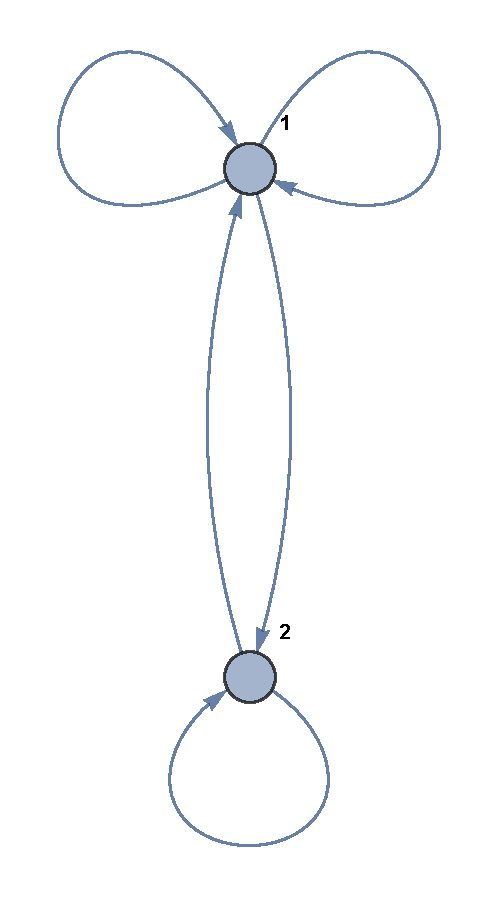
\includegraphics[width=0.80\textwidth]{HLCatMarkovDiagramA}\\(a)
            \end{center}\end{minipage}
            \begin{minipage}[c]{0.25\textwidth}\begin{center}
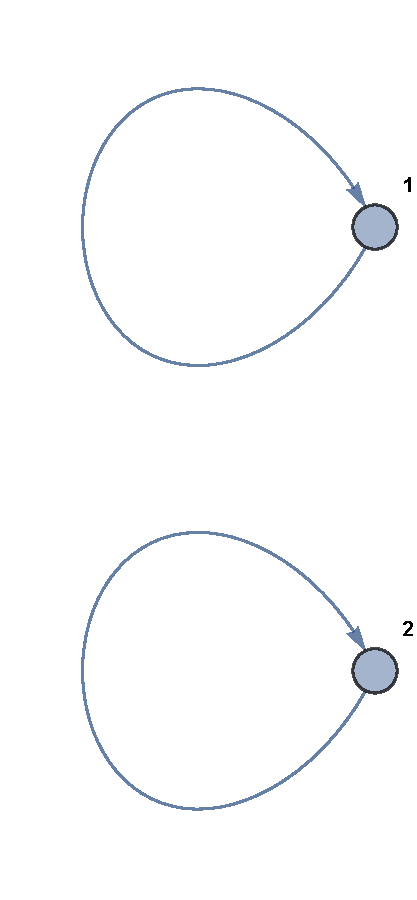
\includegraphics[width=0.80\textwidth]{HLCatMarkovDiagramB}\\(b)
            \end{center}\end{minipage}
            \begin{minipage}[c]{0.2\textwidth}\begin{center}
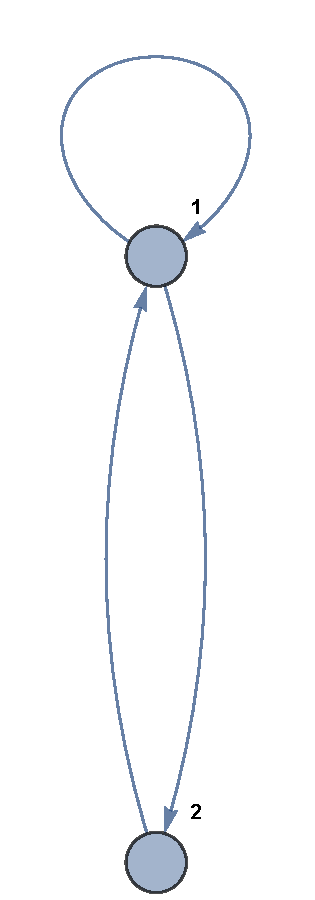
\includegraphics[width=0.80\textwidth]{HLHalfStepCatMarkovDiagramA}\\(c)
            \end{center}\end{minipage}
            ~~~
            \begin{minipage}[c]{0.15\textwidth}\begin{center}
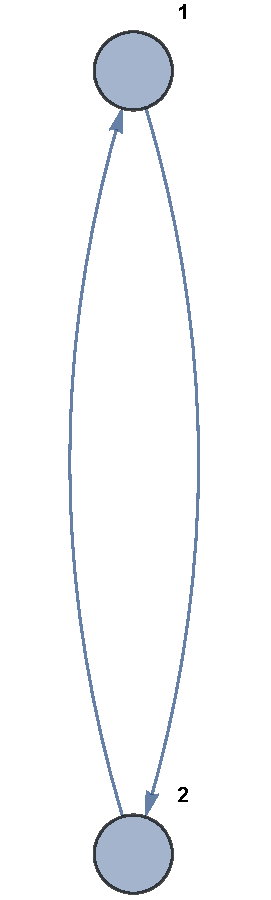
\includegraphics[width=0.80\textwidth]{HLHalfStepCatMarkovDiagramB}\\(d)
            \end{center}\end{minipage}
\end{center}
  \caption{\label{fig:HLHalfStepMarkov}
(a), (b), (c) and (d) are the Markov diagrams corresponding to the transition
matrices $A$, $B$, $A'$ and $B'$. We can get (a) and (b)
by mapping (c) and (d) two time steps forward. $1/\zeta(z)$ is the \tzeta\ of
the Markov diagram (a) with periodic orbits in (b) eliminated.
$1/\tilde{\zeta}(t)$ is the \tzeta\ of
the Markov diagram (c) with periodic orbits in (d) eliminated.
}
\end{figure}
%%%%%%%%%%%%%%%%%%%%%%%%%%%%%%%%%%%%%%%%%%%%%%%%%%%%%%%%%%%%%%%


\beq
\frac{1}{\zeta(z)}
    = \frac{1}{\tilde{\zeta}(t)\tilde{\zeta}(-t)}
    =  \frac{1 - t - t^2}
                  {(1 - t)^2}
        \cdot
        \frac{1 + t - t^2}
                  {(1 + t)^2}
    =  \frac{1 - 3 z + z^2}
                  {(1 - z)^2}
\,,
\ee{AABHM99-46}
where $z=t^2$.

   \item[2021-04-03 Predrag]
The {\henlatt}
\refeq{EG05:ar_pres} is a 3-term recurrence relation of form \refeq{Henlatt-2-step}
\beq
\field_{i+1} +\field_{i}^2 +\field_{i-1}=a  \, ,
\quad i=1,...,n_p
\,.
\label{groups:Henlatt-2-step}
\eeq

\end{description}


%%%%%%%%%%%%%%%%%%%%%%%%%%%%%%%%%%%%%%%%%%%%%%%%%%%%%%%%%%%%%%%%%%%%%%%%%%
\section{Symmetry factorization blog}
\label{sect:symmFactBlog}

\hfill   {\color{red} For the latest entry, go to the bottom of this section}

\bigskip


\begin{description}

    \PCpost{2018-09-02}{
Miles\rf{Miles15}
{\em A dynamical zeta function for group actions},
\\
\arXiv{1506.08555}: ``
introduces and investigates the basic features of a dynamical zeta
function for group actions, motivated by the classical dynamical zeta
function of a single transformation. A product formula for the dynamical
zeta function is established that highlights a crucial link between this
function and the zeta function of the acting group.

The zeta function of a dynamical system is a fundamental invariant that
has warranted considerable attention since the definitive work of Artin
and Mazur\rf{ArtMaz65}. Ruelle\rf{Ruelle02} provides an introduction to
various guises of this function, and Sharp\rf{Sharp04}
(seems to be lacking from
\HREF{https://warwick.ac.uk/fac/sci/maths/people/staff/richard_sharp/p2/}
{here}) provides a
comprehensive survey by  in the context of periodic orbits of hyperbolic
flows.
''

``
The relevance of the dynamical zeta function in questions of orbit growth
is also considered.
''
    }

\item[2020-09-24, 2020-12-16 Predrag to Robert S. MacKay]
(see discussion around \refeq{CatMap2dRSM})
My thoughts in that directions (that is in my \templatt\ talk,
and in this blog, see
\refeq{FGHLW74:charFunct1d},
\refeq{AABHM99-56a},
\refeq{AABHM99-56d},
\refeq{PCcatLattZeta1})
are that for the 1\dmn\ {\templatt}\rf{GHJSC16,CL18}
\beq
       \ssp_{n,\zeit+1} + \ssp_{n,\zeit-1}
- 2\Refl \, \ssp_{\zeit}
     + \ssp_{n+1,\zeit} + \ssp_{n-1, \zeit}
     = -\Ssym{\zeit}
\,,\qquad \Ssym{\zeit}\in\A
\,,
\ee{CatMap2dGroups}
with alphabet
\beq
 \A  =
 \{-{3},-{2},-{1},
   0,\cdots,
   {\mu}^2+1,{\mu}^2+2,{\mu}^2+3\}
\,,
\ee{catLatt2dGroups}
and the Yukawa mass squared of the scalar field $\ssp$
\beq
   {\mu}^2 = 2(\Refl-2)
\,.
\ee{catlattMassGroups}
The $\zeta$ function has to satisfy all {\spt} symmetries of the square
lattice
\beq
%C_{4v} =
\Dn{4} = \{
1, \shift, \shift^2, \shift^3,
\Refl, \Refl_{1},
\Refl_{2},\Refl_{3},
%E, C_{4z}^+, C_{4z}^-, C_{2z}
%\sigma_{y}, \sigma_{x},
%\sigma_{a},\sigma_{b},
\}
\,.
\ee{eq:D4}
See \toChaosBook{section.Y.1} {sect.~A25.1}.

In the international crystallographic notation, this square lattice space
point group is referred to as $p4mm$\rf{Dresselhaus07}.

\item[2019-01-28 Predrag]                                   \toCB
Useful wikis:

\HREF{http://mathworld.wolfram.com/DihedralGroupD4.html}
    {Dihedral group \Dn{4}}

Wolfram Demonstrations:\\
\HREF{https://demonstrations.wolfram.com/DihedralGroupNOfOrder2n/}
{Dihedral Group n of Order 2n}
\\
\HREF{https://demonstrations.wolfram.com/%
CosineAndSineIdentitiesWithDihedralTransformations/}
{Cosine and Sine Identities with Dihedral Transformations}

\HREF{https://en.wikipedia.org/wiki/Examples_of_groups\#The_symmetry_group_of_a_square:_dihedral_group_of_order_8}
{The symmetry group of a square}:
% within\HREF{http://en.wikipedia.org/wiki/Examples_of_groups}{Examples of groups}
I find their ``different Cayley graph'' interesting:
here \Dn{4} is generated by a horizontal (short axis) reflection,
and a diagonal  (long axis)  reflection, rather than the usual $(r,s)$ set.

\HREF{https://groupprops.subwiki.org/wiki/Linear_representation_theory_of_dihedral_groups}
{Linear representation theory of dihedral groups} summarizes everything worth knowing:


\item[2021-01-08 Predrag] taken from
\toChaosBook{rmark.11.2} {remark~11.2}:
{\em Examples of systems with discrete symmetries.}

$\Dn{2}=\Cn{2v} = V_4 =\Ztwo\times \Ztwo$ symmetry
in the stadium billiard\rf{robb}.
Cvitanovi{\'c}, Davidchack  and Siminos\rf{SCD07}
\HREF{http://chaosbook.org/~predrag/papers/SCD07.pdf\#equation.2.13}{eq.~(2.13)}

See \toChaosBook{section.Y.2} {sect.~A25.2}.

$\Dn{4}=\Cn{4v}$ symmetry: in quartic oscillators\rf{EckHoPo89,MaWaRe89},
in the pure $x^2 y^2$ potential\rf{MaSaTAS81,CaPe84} and
in hydrogen in a magnetic field\rf{EckWi90}.

$\Dn{n}$ symmetry: see
\HREF{http://chaosbook.org/projects/dingThesis.pdf\#exmple.2.9}
{Ding thesis example~2.9.}\\
Pdflatex \emph{siminos/lyapunov/blog.tex}, read sect.~7.11.2
\emph{Factorization of $\Cn{n}$ and $\Dn{n}$}.

\item[2020-12-20 Predrag]
This square lattice symmetry group is the space group $p4mm$, with point
group $\Dn{4}$ \refeq{eq:D4}, so all calculations should be
carried out on the reciprocal lattice, with a 1/8th of a square Brilluion
zone, \reffig{fig:SquareBrillouin}.

%%%%%%%%%%%%%%%%%%%%%%%%%%%%%%%%%%%%%%%%%%%%%%%%%%%%%%%%%%%%
\begin{figure}
  \centering
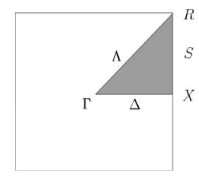
\includegraphics[width=0.38\textwidth]{SquareBrillouin}
  \caption{
The shaded (or yellow) area indicates a \emph{fundamental domain}, \ie, the
smallest part of the pattern whose repeats tile the entire plane.
For the most symmetric 2D square lattice, with point group $p4mm$, the
{fundamental domain} is indicated by the shaded triangle $\Gamma\Lambda
RSX\Delta\Gamma$ which constitutes 1/8 of the Brillouin zone, and contains
the basic wave vectors and the high symmetry points
(Fig.~10.2 of Dresselhaus \etal\rf{Dresselhaus07}).
  }\label{fig:SquareBrillouin}
\end{figure}
%%%%%%%%%%%%%%%%%%%%%%%%%%%%%%%%%%%%%%%%%%%%%%%%%%%%%%%%%%%%%%

Furthermore, one should quotient the \templatt\ \refeq{CatMap2dRSM} by its
$\Dn{1}=\{e,\sigma\}$ \emph{dynamical} symmetry
\beq
\sigma \ssp_\zeit = 1-\ssp_\zeit
    \,,\quad
\sigma \Ssym{\zeit} = {\mu}^2-\Ssym{\zeit}
    \,,\qquad
\mbox{ for all } \zeit\in\integers
\,,
\ee{dynD_1}
where $\Ssym{\zeit}$ takes values in the $\Refl$-letter alphabet
\refeq{catLatt2dRSM}.
Define the fundamental domain to be ${\sspRed}_\zeit\in[0,1/2]$.
We construct the
{\templatt} fundamental domain lattice system, with `1/2' unit hypercube
$\hat{\Xx}\in[0,1/2]^\cl{}$, as in
\toChaosBook{exmple.11.3}
{{\em Group \Dn{1} and reduction to the fundamental domain}},
see \reffig{fig:fig_d_2half}\,(b),
and the fundamental domain symbolic dynamics $\hat{\A}$.
That leads to
\toChaosBook{chapter.25}{chapter 25} \emph{Discrete symmetry
factorization} of zeta functions.

\item[2021-06-08 Predrag]

    \begin{description}
        \item[\HREF{https://web.microsoftstream.com/video/
40585b97-f2cd-4855-a0dc-4d006a919e1d}
        {\raisebox{-0.4ex}{
\includegraphics[width=11pt]{MSteams}}}] {\em
Lecture 7} (Unedited as of 2021-06-18)
        \item[$\circ$]
We work out the symmetry reduction and a breaking of the \Dn{3} symmetry in the
$[3\times3]$ permutation matrices representation
    \end{description}

\item[2021-06-20 Predrag]
I'll have to rerecord the above video from scratch, \refexam{exam:D3permRep}
discussion of the \Dn{3} symmetry is much more compact and elegant.

\item[2021-06-20 Predrag]
This analysis of \Dn{\cl{}} irreps does not apply to symmetric orbits. For
that on has to look at the subgroup structure of dihedral groups, see
\HREF{https://groupprops.subwiki.org/wiki/Subgroup_structure_of_dihedral_groups}
{groupprops wiki}, the subgroup called there $\langle x \rangle$. Han's
discussion of \refeq{HLreflect6}, \refeq{HLreflect6other} and
\refeq{orbJprimeRptHL} counts the broken rotational invariance solutions.

\item[2021-06-21 Predrag]
\HREF{http://www.math.umn.edu/~garrett/} {Paul Garrett} (2014) course notes
\HREF{http://www-users.math.umn.edu/~garrett/m/repns/notes_2014-15/02_dihedral.pdf}
{{\em Harmonic analysis of dihedral group}}
contain a nice discussion of use of discrete Fourier basis for representation
of fields (\ie, scalar functions) on \Dn{\cl{}} lattices.
His \HREF{http://www-users.math.umn.edu/~garrett/m/repns/}
{{\em Representation theory}} course contains many interesting nuggets.

\item[2018-07-04 Predrag] %date ??
Siemaszko and Wojtkowski\rf{SieWoj11} {\em Counting {Berg} partitions} describe
symmetries of \AW\ partitions. They are present for reversible toral
automorphisms.

\item[2021-07-04 Predrag]
The full symmetry group of a toral automorphism was studied by
Baake and Roberts\rf{BaaRob97}.

\item[2021-07-04 Predrag]
The \emph{infinite dihedral group} $\Dn{\infty}$ \refeq{D_infty} was
introduced by Kim, Lee and Park\rf{KiLePa03} {\em A zeta function for flip
systems} (2003).

Kim, Lee and Park\rf{KiLePa03} give the explicit formula \refeq{Ryu17eq:2.1}
for the Lind zeta function\rf{Lind96} $\zeta_{\Refl}$ (search for ``Lind96''
to find more about it) of a flip system $(\pS,\map,\Refl)$
\refeq{Ryu17eq:1.1}.

[...]
investigate dynamical systems with flip maps \refeq{Ryu17eq:1.1}, regarded as
infinite dihedral group actions. We introduce a zeta function for flip
systems, and find its basic properties including a product formula. When the
underlying \Cn{n}-action is conjugate to a topological Markov shift, the flip
system is represented by a pair of matrices, and its zeta function is
expressed explicitly in terms of the representation matrices.

[...]
Any topological Markov shift whose transition matrix is symmetric has a
natural flip.

[...]
establish a zeta function for flip systems which is a conjugacy invariant,
and give a finite description of the function when the underlying
$\integers$-action is conjugate to a topological Markov shift.

\item[2021-07-04 Predrag]
The much desired -see \refeq{EGfactorSincExcl}- square root and
dependence on $t^2$ finally makes an
appearance in the Lind zeta function \refeq{Ryu17eq:2.1}!

\item[2021-07-04 Predrag]
S. Ryu {\em The Lind Zeta functions of reversal systems of finite order}
\arXiv{1712.03519} (2017) deals with a more general case of reversing operators,
but the LaTeX file was useful for clip \& paste.

If $(\pS,\map)$ is a shift of finite type, then there exists a square matrix
$A$ with non-negative integer entries such that the number of fixed points
$N_\cl{}$ can be expressed in terms of matrices\rf{LindMar95}
\begin{equation}\label{Ryu17eq:2.2}
N_\cl{} = \tr A^\cl{} \qquad (m = 1, 2, \cdots)
\end{equation}
Similarly, when $(\pS,\map,\Refl)$ is a shift-flip system of finite type, the
number of fixed points $N^{\Refl}_\cl{}$ can be expressed in terms of
matrices\rf{KiLePa03}. %, {KR}.

They write:
``
Since there is a dynamical system (X, T) which is not conjugate to its
time reversal $(X, T^{-1})$, not every dynamical system has a flip. See
p.~104 of Boyle, Marcus and Trow\rf{BoMaTr987}.
\\
\textbf{Note}: Predrag does not understand that page. Worse still,
Predrag does not understand any page in the entire monograph :(

In Park\rf{Park88} it is shown that if the underlying $\integers$-actions
are Kolmogorov and isomorphic, there are examples of non-isomorphic
\Dn{\infty}-actions.
''

\item[2021-08-11 Predrag]
Park\rf{Park88} {\em On ergodic foliations} (1988).

The `covering space' has two actions, $\map$ and $\Refl$, where $\map$ is
a $\integers$-action, $\Refl$ is a map of order two, and $\Refl$ and T
skew-commute; that is, $\Refl\map\Refl = \map^{-l}$.
\\
\textbf{Note}: Predrag does not understand this paper, not at all.

\item[2021-07-04 Predrag]
Still to read:

Boyle, Marcus and Trow\rf{BoMaTr987}
{\em Resolving maps and the dimension group for shifts of finite type}
(1987).

Nordin and Noorani\rf{NorNoo21}
{\em Counting finite orbits for the flip systems of shifts of finite type}
(2021).

Yumiko Hironaka
{\em Zeta functions of finite groups by enumerating subgroups},
\arXiv{1410.4326} (2014) is potentially interesting: Hironaka forms zeta
function like Riemann, rather than  Artin-Mazur.

Richard Miles
{\em Orbit growth for algebraic flip systems}
\HREF{https://doi.org/10.1017/etds.2014.38} {DOI} (2014)

Sieye Ryu
\HREF{https://hdl.handle.net/10371/121280} {PhD thesis}
{{\em The Lind Zeta Function and Williams' Decomposition Theorem for Sofic
Shift-Reversal Systems of Finite Order}}
 (2014)

Golubitsky and Stewart\rf{golubitsky2002sp}
{{\em The Symmetry Perspective}},
chapters {\em Time Periodicity and Spatio-Temporal Symmetry}
and
{\em Periodic Solutions of Symmetric Hamiltonian Systems}
(2002)

\end{description}


%%%%%%%%%%%%%%%%%%%%%%%%%%%%%%%%%%%%%%%%%%%%%%%%%%%%%%%%%%%%%
\fastTrackExam{exam:Symm1d}     % \toExam
%%%%%%%%%%%%%%%%%%%%%%%%%%%%%%%%%%%%%%%%%%%%%%%%%%%%%%%%%%%%%
%
%%%%%%%%%%%%%%%%%%%%%%%%%%%%%%%%%%%%%%%%%%%%%%%%%%%%%%%%%%%%%
\fastTrackExam{exam:Fact1d}     % \toExam
%%%%%%%%%%%%%%%%%%%%%%%%%%%%%%%%%%%%%%%%%%%%%%%%%%%%%%%%%%%%%

%%%%%%%%%%%%%%%%%%%%%%%%%%%%%%%%%%%%%%%%%%%%%%%%%%%%%%%%%%%%%
% \example{\Dn{3} multiplication tables and the permutation rep.}
\fastTrackExam{exam:D3permRep}     % \toExam
%%%%%%%%%%%%%%%%%%%%%%%%%%%%%%%%%%%%%%%%%%%%%%%%%%%%%%%%%%%%%
%
%%%%%%%%%%%%%%%%%%%%%%%%%%%%%%%%%%%%%%%%%%%%%%%%%%%%%%%%%%%%%
% \example{\Dn{6} multiplication tables.}
\fastTrackExam{exam:D6mult}     % \toExam
%%%%%%%%%%%%%%%%%%%%%%%%%%%%%%%%%%%%%%%%%%%%%%%%%%%%%%%%%%%%%
%
%%%%%%%%%%%%%%%%%%%%%%%%%%%%%%%%%%%%%%%%%%%%%%%%%%%%%%%%%%%%%
% \example{\Dn{6} permutation rep.}
\fastTrackExam{exam:D6permRep}     % \toExam
%%%%%%%%%%%%%%%%%%%%%%%%%%%%%%%%%%%%%%%%%%%%%%%%%%%%%%%%%%%%%

\newpage
% siminos/spatiotemp/chapter/symGroupXD.tex
% $Author: predrag $ $Date: 2021-08-03 16:02:22 -0400 (Tue, 03 Aug 2021) $

\section{Group theory and symmetries: a review}
\label{sect:group}

    \PC{2021-06-19}{
    A copy of the 2017-03-09 section from Xiong Ding's thesis\\
    siminos/xiong/thesis/chapters/symGroup.tex.
    }
    \PC{2021-06-19}{
    Update/replace the ChaosBook version, as now
    $\Zn{2}\to\Dn{1}, \Zn{3}\to\Cn{3}$.
    }
In quantum mechanics, whenever a system exhibits some symmetry, the
corresponding symmetry group commutes with the Hamiltonian of this
system, namely, $[U(\LieEl), H] = U(\LieEl)H - HU(\LieEl) = 0$. Here
$U(\LieEl)$ denotes the operation corresponding to symmetry $g$ whose
meaning will be explained soon. The set of eigenstates with degeneracy
$\ell$, $\{\phi_1, \phi_2, \cdots, \phi_\ell\}$, corresponding to the same
system energy $H\psi_i = E_n\psi_i$, is invariant under the symmetry
since $U(\LieEl)\psi_i$ are also eigenvectors for the same energy.
This information helps us understand the spectrum of a Hamiltonian and
the quantum mechanical selection rules. We now apply the same idea to
the classical {\evOper} $\Lop^t(\ssp_e, \ssp_s)$
for a system $\flow{t}{\ssp}$ equivariant under a discrete symmetry group
$\Group=\{e, \LieEl_2, \LieEl_3,\cdots, \LieEl_{|\Group|}\}$ of order
$|\Group|$:
\begin{equation}
  \label{eq:equiva}
  \flow{t}{{D}(\LieEl)}\ssp)={D}(\LieEl)\,\flow{t}{\ssp} \quad \text{for}
  \quad \forall
  \LieEl\in\Group
  \,.
\end{equation}
We start with a review of some basic facts of
the group representation theory. Some examples of good references
on this topic are \refref{Hamermesh62, Tinkham}.

Suppose group $\Group$ acts on a linear space $V$ and function
$\rho(\ssp)$ is defined on this space $\ssp\in V$. Each element
$\LieEl\in\Group$ will transform point $\ssp$ to ${D}(\LieEl)\ssp$. At
the same time, $\rho(\ssp)$ is transformed to $\rho'(\ssp)$. The value
$\rho(\ssp)$ is unchanged after state point $\ssp$ is transformed to
${D}(\LieEl)\ssp$, so $\rho'({D}(\LieEl)\ssp) = \rho(\ssp)$. Denote
$U(\LieEl)\rho(\ssp)=\rho'(\ssp)$, so we have
\begin{equation}
  \label{eq:ogfx}
  U(\LieEl)\rho(\ssp) = \rho({D}(\LieEl)^{-1}\ssp)
  \,.
\end{equation}
This is how functions are transformed by group operations. Note, $D(\LieEl)$
is the representation of $G$ in the form of space transformation matrices.
The
operator $U(\LieEl)$, which acts on the function space, is not the same as
group operation ${D}(\LieEl)$, so \refeq{eq:ogfx} does not mean that
$\rho(\ssp)$ is invariant under $\Group$. \refExam{exam:C3matrRep} gives
the space transformation matrices of $\Cn{3}$.

%%%%%%%%%%%%%%%%%%%%%%%%%%%%%%%%%%%%%%%%%%%%%%%%%%%%%%%%%%%%%
% \example{A matrix representation of cyclic group $\Cn{3}$.}
\fastTrackExam{exam:C3matrRep}     % \toExam
%%%%%%%%%%%%%%%%%%%%%%%%%%%%%%%%%%%%%%%%%%%%%%%%%%%%%%%%%%%%%

\subsection{Regular representation}
An operator $U(\LieEl)$ which acts on an infinite\dmn\ function space
is too abstract to analyze.
We would like to represent it in a more familiar way.
Suppose there is a function $\rho(\ssp)$ with symmetry $\Group$ defined in full
\statesp\ $\pS$, then full \statesp\ can be decomposed as a union
of $|\Group|$ tiles each of which is obtained by transforming the fundamental
domain,
\begin{equation}
  \label{eq:domain}
  \pS =  \bigcup_{g\in \Group}g\pSRed
  \,,
\end{equation}
where $\pSRed$ is the chosen fundamental domain.
So $\rho(\ssp)$ takes $|G|$ different forms by \refeq{eq:ogfx} in each sub-domain
in \refeq{eq:domain}. Now, we obtained a natural choice of a set of bases in this
function space called the \emph{regular basis},
\beq
\label{eq:RegBasis}
\{ \rho_1^{reg}(\sspRed), \rho_2^{reg}(\sspRed), %\rho_3^{reg}(\sspRed),
\cdots, \rho_{|\Group|}^{reg}(\sspRed)\}
=
\{
\rho(\sspRed), \rho(\LieEl_2\sspRed), % \rho(\LieEl_3\sspRed),
\cdots, \rho(\LieEl_{|\Group|}\sspRed) \}
\,.
\eeq
Here, for notation simplicity we use
$\rho(\LieEl_i\sspRed)$ to represent $\rho(D(\LieEl_i\sspRed))$ without
ambiguity.
These bases are
constructed by applying $U(\LieEl^{-1})$ to $\rho(\sspRed)$ for each
$\LieEl\in\Group$, with $\sspRed$ a point in the fundamental domain.
The [$|G|\!\times\!|G|$] matrix representation of the
action of $U(\LieEl)$ in basis \refeq{eq:RegBasis} is called the \emph{(left)
regular representation} $D^{reg}(\LieEl)$. Relation \refeq{eq:ogfx} says that
$D^{reg}(\LieEl)$ is a permutation matrix, so each row or column has only one nonzero
element.

We have a simple trick to obtain the regular representation quickly.
Suppose the element at the $i$th row and
the $j$th column of $D^{reg}(\LieEl)$
is $1$. It means
$\rho(\LieEl_i\sspRed) = U(\LieEl) \rho(\LieEl_j\sspRed)$, which
is $g_i=\LieEl^{-1}g_j \implies g^{-1} = g_i g_j^{-1}$. Namely,
\beq
D^{reg}(\LieEl)_{ij} = \delta_{\LieEl^{-1},\, g_i g_j^{-1}}
\,.
\ee{eq:RegRep}
So if we arrange the
columns of the multiplication table by the inverse of the group elements,
then setting positions with $\LieEl^{-1}$ to 1 defines the regular
representation $D^{reg}(\LieEl)$. Note, the above relation can
be further simplified to $g = g_jg_i^{-1}$, but it exchanges the rows and
columns of the multiplication table, so $g = g_jg_i^{-1}$
should not be used to get $D^{reg}(\LieEl)$.
On the other hand, it is easy to see
that the regular representation of group element $e$ is always the identity matrix.

%%%%%%%%%%%%%%%%%%%%%%%%%%%%%%%%%%%%%%%%%%%%%%%%%%%%%%%%%%%%%%%%%%%%%%
% \example{The regular representation of cyclic group $\Cn{3}$.}
\fastTrackExam{exam:C3regularRep}     % \toExam
%%%%%%%%%%%%%%%%%%%%%%%%%%%%%%%%%%%%%%%%%%%%%%%%%%%%%%%%%%%%%

\subsection{Irreducible representations}

$U(\LieEl)$ is a linear operator under the regular basis.
Any linearly independent combination of the regular bases can be used as
new basis, and then the representation of $U(\LieEl)$ changes respectively.
So we ask a question: can we find a new set of bases
\begin{equation}
  \rho^{irr}_i=\sum_j S_{ij}\rho^{reg}_j
  \label{eq:trans}
\end{equation}
such that the new representation $D^{irr}(\LieEl) = SD^{reg}(\LieEl)S^{-1}$ is block-diagonal
for any $\LieEl\in\Group$ ?
\begin{equation}
  D^{irr}(\LieEl) =
  \begin{bmatrix}
    D^{(1)}(\LieEl) & & \\
    & D^{(2)}(\LieEl) & \\
    & & \ddots \\
  \end{bmatrix}
  = \bigoplus_{\mu=1}^\shift d_\mu D^{(\mu)}(\LieEl)
  \,.
  \label{eq:irre}
\end{equation}
In such a block-diagonal representation, the
subspace corresponding to each diagonal block is invariant under $\Group$
and the action of $U(\LieEl)$ can be analyzed subspace by subspace.
It can be easily checked that for each $\mu$, $D^{(\mu)}(\LieEl)$ for all
$\LieEl\in\Group$ form another representation (\emph{irreducible
  representation}, or \emph{irrep}) of group $\Group$.
Here, $r$ denotes the total number of
irreps of $\Group$. The same irrep may show up more than once in the decomposition
\refeq{eq:irre}, so the coefficient $d_{\mu}$ denotes the number of its
copies.  Moreover, it is proved\rf{Hamermesh62} that $d_{\mu}$ is also equal to the dimension
of $D^{(\mu)}(\LieEl)$ in \refeq{eq:irre}.
Therefore, we have a relation
\[
  \sum_{\mu=1}^r d_\mu^2 = |G|
  \,.
\]

%%%%%%%%%%%%%%%%%%%%%%%%%%%%%%%%%%%%%%%%%%%%%%%%%%%%%%%%%%%%%%%%%%%%%%
% \example{Irreps of cyclic group $\Cn{3}$.}
\fastTrackExam{exam:C3irReps}     % \toExam
%%%%%%%%%%%%%%%%%%%%%%%%%%%%%%%%%%%%%%%%%%%%%%%%%%%%%%%%%%%%%

\paragraph{Character tables.}
Finding a transformation $S$ which simultaneously block-diagonalizes the
regular representation of each group element sounds difficult.
However, suppose it can be achieved and we obtain a set of irreps $D^{(\mu)}(\LieEl)$,
then according to Schur's lemmas\rf{Hamermesh62}, $D^{(\mu)}(\LieEl)$ must satisfy a set of
orthogonality relations:
\begin{equation}
  \label{eq:ortho}
  \frac{d_\mu}{|G|} \sum_g D_{il}^{(\mu)}(\LieEl) D_{mj}^{(\nu)}(g^{-1}) = \delta_{\mu \nu}
  \delta_{ij} \delta_{lm}
  \,.
\end{equation}
Denote the trace of irrep $D^{(\mu)}$ as $\chi^{(\mu)}$, which is referred to as
the \emph{character} of $D^{(\mu)}$. Properties of irreps can be derived from
\refeq{eq:ortho}, and we list them as follows:
\begin{enumerate}
\item The number of irreps is the same as the number of
  classes.
\item Dimensions of irreps satisfy
  $\sum_{\mu=1}^\shift d^2_\mu = |G| $
\item Orthonormal relation I :
  $\sum_{i=1}^\shift |K_i| \chi_i^{(\mu)} \chi_i^{(\nu)*} = |G|\delta_{\mu \nu} $. \\
  Here, the summation goes through all classes of this group, and $|K_i|$ is
  the number of elements in class $i$. This weight comes from the fact that
  elements in the same class have the same character. Symbol $*$ means
  the complex conjugate.
\item Orthonormal relation II :
  $\sum_{\mu=1}^\shift \chi_i^{(\mu)} \chi_j^{(\mu)*} = \frac{|G|}{|K_i|}\delta_{ij} $. \\
\end{enumerate}
The characters for all classes and irreps of a finite group are
conventionally arranged into a \emph{character table}, a square matrix
whose rows represent different
classes and columns represent different irreps.
Rules 1 and 2 help determine the number of irreps and
their dimensions. As the matrix representation of class $\{e\}$ is always the
identity matrix, the first row is always the dimension of the
corresponding representation. All entries of the first column are always 1,
because the symmetric irrep is always one\dmn. To compute the
remaining entries, we should use properties 3, 4 and the class multiplication
tables.   Spectroscopists conventions use labels $A$ and $B$ for
symmetric, respectively antisymmetric nondegenerate irreps, and
$E$, $T$, $G$, $H$ for doubly, triply, quadruply, quintuply degenerate irreps.

%%%%%%%%%%%%%%%%%%%%%%%%%%%%%%%%%%%%%%%%%%%%%%%%%%%%%%%%%%%%%%%%%%%%%%
% \example{Character table of $\Dn{3}$.}
\fastTrackExam{exam:D3charTab}     % \toExam
%%%%%%%%%%%%%%%%%%%%%%%%%%%%%%%%%%%%%%%%%%%%%%%%%%%%%%%%%%%%%

\subsection{Projection operator}
We have listed the properties of irreps and the
techniques of constructing a character table, but we still do not know how to
construct the similarity transformation $S$ which takes a regular representation into a
block-diagonal form. Think of it in another way,
each irrep is associated with an invariant subspace, so by
projecting an arbitrary function $\rho(\ssp)$ into its invariant subspaces, we
find the transformation \refeq{eq:trans}.
One of these invariant subspaces is $\sum_g \rho(g\sspRed)$, which is the basis of
the one\dmn\ symmetric irrep $A$. For $\Cn{3}$, it is \refeq{eq:c3f1}.
But how to get the others? We resort to the projection operator:
\begin{equation}
  \label{eq:projecIrre}
  P^{(\mu)}_{i} = \frac{d_\mu}{|G|}\sum_g \left(D^{(\mu)}_{ii} (\LieEl)\right)^* U(g)
  \,.
\end{equation}
It projects an arbitrary function into the $i$th basis of irrep
$D^{(\mu)}$ provided the diagonal elements of this representation
$D^{(\mu)}_{ii}$ are known. $ P^{(\mu)}_{i} \rho(\ssp) = \rho^{(\mu)}_i$.
Here, symbol $*$ means the complex conjugate. For unitary groups
$\left(D^{(\mu)}_{ii} (\LieEl)\right)^* = D^{(\mu)}_{ii} (\LieEl^{-1})$.
Summing $i$ in \refeq{eq:projecIrre} gives
\begin{equation}
  \label{eq:projectSum}
  P^{(\mu)} = \frac{d_\mu}{|G|}\sum_g \left(\chi^{(\mu)}(\LieEl)\right)^*U(g)
  \,.
\end{equation}
This is also a projection operator which projects an arbitrary function onto
the sum of the bases of irrep $D^{(\mu)}$.

Note, for one\dmn\ representations, \refeq{eq:projectSum}
is equivalent to \refeq{eq:projecIrre}. The projection operator is
known after we obtain
the character table, since the character of an one\dmn\ matrix is the matrix itself.
However, for two\dmn\ or higher\dmn\ representations, we need to know the
diagonal elements $D^{(\mu)}_{ii}$ in order to get the basis of invariant subspaces. That is to say,
\refeq{eq:projecIrre} should be used instead of \refeq{eq:projectSum} in this case.
\refExam{exam:D3irrepBases} illustrates this point. The two one\dmn\ irreps are obtained
by \refeq{eq:projectSum}, but the other four two\dmn\ irreps are obtained by
\refeq{eq:projecIrre}.

%%%%%%%%%%%%%%%%%%%%%%%%%%%%%%%%%%%%%%%%%%%%%%%%%%%%%%%%%%%%%%%%%%%%%%
% \example{Bases for irreps of $\Dn{3}$.}{
\fastTrackExam{exam:D3irrepBases}     % \toExam
%%%%%%%%%%%%%%%%%%%%%%%%%%%%%%%%%%%%%%%%%%%%%%%%%%%%%%%%%%%%%

The $\Cn{3}$ and $\Dn{3}$ examples used in this section can be
generalized to any $\Cn{n}$ and $\Dn{n}$. For references,
\refExam{exam:CnChars}, \refexam{exam:DnOddChars} and
\refexam{exam:DnEvenChars} give the character tables of $\Cn{n}$ and
$\Dn{n}$.

%%%%%%%%%%%%%%%%%%%%%%%%%%%%%%%%%%%%%%%%%%%%%%%%%%%%%%%%%%%%%%%%%%%%%%
% \example{Character table of cyclic group \Cn{n}.}
\fastTrackExam{exam:CnChars}     % \toExam
%%%%%%%%%%%%%%%%%%%%%%%%%%%%%%%%%%%%%%%%%%%%%%%%%%%%%%%%%%%%%
%
%%%%%%%%%%%%%%%%%%%%%%%%%%%%%%%%%%%%%%%%%%%%%%%%%%%%%%%%%%%%%%%%%%%%%%
% \example{Character table of dihedral group $\Dn{n}$, $n$ odd.}
\fastTrackExam{exam:DnOddChars}     % \toExam
%%%%%%%%%%%%%%%%%%%%%%%%%%%%%%%%%%%%%%%%%%%%%%%%%%%%%%%%%%%%%
%
%%%%%%%%%%%%%%%%%%%%%%%%%%%%%%%%%%%%%%%%%%%%%%%%%%%%%%%%%%%%%
% \example{Character table of dihedral group $\Dn{n}$, $n$ even.}
\fastTrackExam{exam:DnEvenChars}     % \toExam
%%%%%%%%%%%%%%%%%%%%%%%%%%%%%%%%%%%%%%%%%%%%%%%%%%%%%%%%%%%%%


%%%%%%%%%%%%%%%%%%%%%%%%%%%%%%%%%%%%%%%%%%%%%%%%%%%%%%%%%%%%%%%%%%%%%%%%%%%%%
\Remarks

%%%%%%%%%%%%%%%%%%%%%%%%%%%%%%%%%%%%%%%%%%%%%%%%
\remark{Time reversal.}{\label{rem:timeRev}
\index{lattice!time reversal}\index{time reversal!lattice}
% 2021-01-27 Predrag
Some background on $\Dn{\infty}$ symmetry of the \templatt\ and
{$\phi^4$} 1$d$ lattice field theory, \refsect{s:latt1d} {\em
Translations and reflections}. Time-reversed {\lattstate}s (if not
self-dual under reflection) are counted as pairs, see for example
\toChaosBook{figure.caption.192} {fig. 11.6},
\toChaosBook{exmple.11.11} {example~11.11},
\toChaosBook{exmple.15.6}{Example 15.6} {\em \Cn{2} recoded},
\toChaosBook{figure.caption.308} {fig.~15.15},
\toChaosBook{table.caption.362}{table~18.1}
{\em The 4-disk {\orbit}s up to period 8},
\toChaosBook{table.caption.556}{table~34.1},
the time-reversal discussion in
\toChaosBook{subsection.42.2.3} {section~42.2.3},
and
\toChaosBook{figure.caption.608} {fig.~42.5}.

This is a many-years outstanding frustration, see
\toChaosBook{rmark.16.3} {Remark 16.3} {\em Symmetries of the symbol square}
and
\toChaosBook{rmark.25.2} {Remark 25.2} {\em Other symmetries}.

The zeta functions are still to be factorized in the $z\to{t^2}$ sense,
perhaps as in \refeq{AABHM99-46a}. Then the corresponding ChaosBook
chapters have to be rewritten.
} %end %\remark{rem:timeRev}
%%%%%%%%%%%%%%%%%%%%%%%%%%%%%%%%%%%%%%%%%%%%%%%%
\RemarksEnd
%%%%%%%%%%%%%%%%%%%%%%%%%%%%%%%%%%%%%%%%%%%%%%%%%%%%%%%%%%%%%%%%%%%%%%%%%%%%%

\section{Examples}
\label{exam:groups}

%%%%%%%%%%%%%%%%%%%%%%%%%%%%%%%%%%%%%%%%%%%%%%%%%%%%%%%%%%%%%
% examFiniteGr.tex called by \Chapter{finiteGr}{}{Flips, slides and turns}
% REMEMBER to RETURN to ChaosBook
%% Finite groups.
%%  \input{../spatiotemp/Examples/dscrfiniteG}
%% Discrete groups of order 2 on \Rls{3}.  % RETURN to ChaosBook
    % siminos/spatiotemp/Examples/exam3dFlowsDscr.tex
% $Author: predrag $ $Date: 2021-07-24 23:53:43 -0400 (Sat, 24 Jul 2021) $

%%%%%%%%%%%%%%%%%%%%%%%%%%%%%%%%%%%%%%%%%%%%%%%%%%%%%%%%%%%%%%%%%%
\example{Discrete groups of order 2 on \Rls{3}.}{\label{exam:3dFlowsDscr}
% in examFiniteGr.tex, called by \Chapter{finiteGr}{}{Flips, slides and turns}
%                                       \toCB
Three types of discrete group of order 2 can arise by
linear action on our 3\dmn\ Euclidean space \Rls{3}:            \toCB
    % finiteGr3D-D1symms.camproj    recorded 2015-01-29
    % edited DeJuan                          2015-02-24
    % Title: 3D symmetries of order 2
\toVideo{youtube.com/embed/pbBF7EK8X9I} % uploaded 2015-02-24
    %
\bea
\mbox{reflections:  } \Refl (x,y,z) &=& (x,y,-z)
    \continue
\mbox{rotations:      } \shift(x,y,z) &=& (-x,-y,z)
    \label{3dOrder2symm}\\
\mbox{inversions:    } P (x,y,z) &=& {(-x,-y,-z)}
    \nnu
\,.
\eea
\Refl\ is a {\em reflection} (or an inversion) through  the
$[x,y]$ plane.
 $\shift$ is $[x,y]$-plane, constant $z$
{\em rotation} by $\pi$ about the $z$-axis
(or an inversion thorough the $z$-axis).
$P=\shift\Refl$ is an {\em inversion} (or parity operation)
through the point $(0,0,0)$.
Singly, each operation generates a group of order 2:
$ \Dn{1} = \{e , \Refl \}$,
$ \Cn{2}  = \{e,\shift\}$,
and
$\Dn{1} = \{e , P \}$.
Together, they form the dihedral group
$ \Dn{2} = \{e , \Refl, \shift, \Refl\shift\}$
of order 4.
\index{reflection}\index{inversion}
~(continued in \refexam{exam:3dCoordDscr})
                                        \jumpBack{exam:3dFlowsDscr}
        } %end \example{Discrete groups of order 2 on \Rls{3}
%%%%%%%%%%%%%%%%%%%%%%%%%%%%%%%%%%%%%%%%%%%%%%%%%%%%%%%%%%%%%%%%%%

%% Discrete operations on \Rls{3}.  % RETURN to ChaosBook
    % siminos/spatiotemp/Examples/exam3dCoordDscr.tex
% $Author: predrag $ $Date: 2021-07-23 16:24:01 -0400 (Fri, 23 Jul 2021) $

%%%%%%%%%%%%%%%%%%%%%%%%%%%%%%%%%%%%%%%%%%%%%%%%%%%%%%%%%%%%%%%%%%
\example{Discrete operations on \Rls{3}.}{\label{exam:3dCoordDscr}
% in examFiniteGr.tex, called by \Chapter{finiteGr}{}{Flips, slides and turns}
(Continued from \refexam{exam:3dFlowsDscr}.)          \toCB
The matrix representation of reflections, rotations
and inversions defined by \refeq{3dOrder2symm} is
 \beq
 \matrep{\Refl} =   \left(\barr{ccc}
    1  &  0 & ~0  \\
    0  &  1 & ~0 \\
    0  &  0 & -1
    \earr\right)
     ,\quad
 \matrep{\shift} =   \left(\barr{ccc}
    -1  &  ~0 & 0  \\
    ~0  &  -1 & 0 \\
    ~0  &  ~0 & 1
    \earr\right)
     ,\quad
 \matrep{P} =   \left(\barr{ccc}
    -1  &  ~0 & ~0  \\
    ~0  &  -1 & ~0 \\
    ~0  &  ~0 & -1
    \earr\right)
\,,
 \label{3dCoordDiscr}
 \eeq
with $\det{\matrep{\shift}} = 1$,
$\det{\matrep{\Refl}} = \det{\matrep{P}} = -1$; that is why we
refer to $\shift$ as a rotation, and $\Refl$, $P$ as inversions. As
$\LieEl^2 = e$ in all three cases, these are groups of order 2.
~~(continued in \refexam{exam:3dinvDscr})
                                        \jumpBack{exam:3dCoordDscr}
        } %end \example{Discrete operations on \Rls{3}.
%%%%%%%%%%%%%%%%%%%%%%%%%%%%%%%%%%%%%%%%%%%%%%%%%%%%%%%%%%%%%%%%%%

%% Equivariance of the Lorenz flow.  % RETURN to ChaosBook
    % siminos/spatiotemp/Examples/exam3dinvDscr.tex
% $Author: predrag $ $Date: 2021-07-23 16:24:01 -0400 (Fri, 23 Jul 2021) $

%%%%%%%%%%%%%%%%%%%%%%%%%%%%%%%%%%%%%%%%%%%%%%%%%%%%%%%%%%%%%%%%%%%%%%%
\example{Equivariance of the Lorenz flow.}{\label{exam:3dinvDscr}
\index{Lorenz flow!symmetry}
(Continued from \refexam{exam:3dCoordDscr})~~
The velocity field in Lorenz equations  \refeq{Lorenz}
                                                \exerbox{exer:LorenzEqui}
\beq
    \left[
        \begin{array}{c}
\dot{x} \\ \dot{y} \\ \dot{z}
    \end{array}
    \right]
    =
    \left[
        \begin{array}{c}
\sigma (y-x) \\
\rho x - y -xz \\
xy -bz
    \end{array}
    \right]
\ee{finiteGr:Lorenz}
is equivariant under the action of cyclic group % \Ztwo
$\Cn{2} = \{e,\shift{}\}$ acting on \Rls{3}\ by a $\pi$ rotation about the $z$
axis,
\beq
    \shift{}(x,y,z) = (-x,-y,z)\,.
\ee{LorEquiv}
~~(continued in \refexam{exam:LorenzD1})
                                        \jumpBack{exam:3dinvDscr}
        } %end \example{Equivariance of the Lorenz flow
%%%%%%%%%%%%%%%%%%%%%%%%%%%%%%%%%%%%%%%%%%%%%%%%%%%%%%%%%%%%%%%%%%

%% Equivariance of the Lorenz flow.  % RETURN to ChaosBook
    % siminos/spatiotemp/Examples/examLorenzD1.tex
% $Author: predrag $ $Date: 2021-07-25 19:52:46 -0400 (Sun, 25 Jul 2021) $

%%%%%%%%%%%%%%%%%%%%%%%%%%%%%%%%%%%%%%%%%%%%%%%%%%%%%%%%%%%%%%%%%%%%%%%%%%
\example{Desymmetrization of Lorenz flow.}{ \label{exam:LorenzD1}
% from % examDiscrete.tex called by \Chapter{discrete}{}{World in a mirror}
% RETURN!
% Predrag                           04apr2008
% Predrag                           19jan2008
% moved to here from halcrow/blog/TEX/lorenz.tex
\index{Lorenz flow}                                 \toCB
%\PC{2017-07-24}{ChaosBook: start the discrete.tex example here, link to the intro example in
%    the flow.tex chapter}
(Continuation of \refexam{exam:3dinvDscr})~~
Lorenz equation \refeq{finiteGr:Lorenz} is equivariant under \refeq{LorEquiv}, the
action of order-2 group $\Cn{2} = \{e,\shift\}$, where $\shift$ is
$[x,y]$-plane, half-cycle rotation by $\pi$ about the $z$-axis:
\beq
(x,y,z) \to \shift(x,y,z) = (-x,-y,z) \,.
\ee{LorenzR}
$\shift^2=1$ condition decomposes the \statesp\ into two linearly
irreducible subspaces $\pS = \pS^+ \oplus \pS^-$, the $z$-axis $\pS^+$
and the $[x,y]$ plane $\pS^-$, with projection operators onto the two
subspaces given by
      \PublicPrivate{
      }{% switch \PublicPrivate{
(see \refsect{appeStabEigs})
      } % end \PublicPrivate{
 \beq
 \PP^+ = \frac{1}{2}(1 + \shift)
 =   \left(\barr{ccc}
    0  &  0 & 0  \\
    0  &  0 & 0 \\
    0  &  0 & 1
    \earr\right)
     ,\quad
 \PP^- = \frac{1}{2}(1 - \shift)
  =   \left(\barr{ccc}
    1  &  0 & 0  \\
    0  &  1 & 0 \\
    0  &  0 & 0
    \earr\right)
\,.
 \label{projOp:sig}
 \eeq
As the flow is $\Cn{2}$-invariant, so is its linearization $\dot{\ssp} =
\Mvar \ssp$. Evaluated at $\EQV{0}$, $\Mvar$ commutes with  $\shift$,
and, as we have already seen in  \refexam{exam:LorenzStab}, the $\EQV{0}$
{\stabmat} decomposes into $[x,y]$ and $z$ blocks.
    \PC{20171-07-24}{create example in \refsect{s:StabRpo} from the last sentence}

The 1\dmn\ $\pS^+$ subspace is the fixed-point subspace, with the
$z$-axis \emph{point-wise invariant} under the group action
\beq
\pS^+ = \Fix{\Cn{2}} =
   \{ \ssp \in \pS \mid \LieEl  \, \ssp = \ssp \mbox{ for } g \in \{e,\shift\} \}
%\,.
\ee{dscr:LorFPsubsp}
(here $\ssp = (x,y,z)$ is a 3\dmn\ vector, not the coordinate $x$). A
\Cn{2}-fixed point $\ssp(\zeit)$ in $\Fix{\Cn{2}}$ moves with time, but
according to \refeq{flowInv} remains within $\ssp(\zeit) \in \Fix{\Cn{2}}$ for
all times; the  subspace $\pS^+ = \Fix{\Cn{2}}$ is {\em flow invariant}.
In case at hand this jargon is a bit of an overkill: clearly for
$(x,y,z)=(0,0,z)$ the full \statesp\ Lorenz equation \refeq{finiteGr:Lorenz} is
reduced to the exponential contraction to the $\EQV{0}$ \eqv,
\PC{2017-07-24}{pointer to turbulence chapter here}
\beq
\dot{z} = -b \, z
\,.
\ee{LorenzZaxis}
% which is the reason why you never see this decomposition discussed
% in literature. Even though
However, for higher-dim\-ens\-ion\-al flows the flow-invariant subspaces
can be high-dim\-ens\-ion\-al, with interesting dynamics of their own.
Even in this simple case this subspace plays an important role as a
topological obstruction: the orbits can neither enter it nor exit it, so
the number of windings of a trajectory around it provides a natural,
topological symbolic dynamics.

The $\pS^-$ subspace is, however, {\em not} flow-invariant, as the nonlinear
terms $\dot{z}=xy - bz$ in the Lorenz equation \refeq{finiteGr:Lorenz}
send all initial conditions within
$\pS^-=(x(0),y(0),0)$ into the full, $z(\zeit) \neq 0$ \statesp\  $\pS/\pS^+$.
~~(continued in \refexam{exam:LorenzPolarRep})
                                        \jumpBack{exam:LorenzD1}

\hfill   (E. Siminos and J. Halcrow)
    } %end {exam:LorenzD1}
%%%%%%%%%%%%%%%%%%%%%%%%%%%%%%%%%%%%%%%%%%%%%%%%%%%%%%%%%%%%%%%%%%%%%%%%%%

%% Discrete symmetries of the \pCf.  % RETURN to ChaosBook
    % siminos/spatiotemp/Examples/pCfSymmDiscr.tex
% $Author: predrag $ $Date: 2021-07-23 16:24:01 -0400 (Fri, 23 Jul 2021) $

%%%%%%%%%%%%%%%%%%%%%%%%%%%%%%%%%%%%%%%%%%%%%%%%%%%%%%%%%%%%%%%%%%
\example{Discrete symmetries of the \pCf.} {\label{exam:pCfSymmDiscr}
% in examFiniteGr.tex, called by \Chapter{finiteGr}{}{Flips, slides and turns}
     \index{plane Couette flow!symmetries}                     \toCB
The \pCf\ is a fluid flow bounded by two countermoving planes, in a cell
periodic in streamwise and spanwise directions. The Navier-Stokes
equations for the \pCf\  have two discrete symmetries: reflection through
the (streamwise , wall-normal) plane, and rotation by $\pi$ in the
(streamwise , wall-normal) plane. That is why the system has \eqv\ and \po\
solutions, as well as \reqv\ and \rpo\ solutions discussed in
\refchap{c-continuous}). They belong to discrete symmetry subspaces.
~(continued in \refexam{exam:PpCfSymm})
                \jumpBack{exam:pCfSymmDiscr}
        } %end \example{exam:pCfSymmDiscr}
%%%%%%%%%%%%%%%%%%%%%%%%%%%%%%%%%%%%%%%%%%%%%%%%%%%%%%%%%%%%%%%%%%

%% A reflection symmetric $1d$ map.  % RETURN to ChaosBook
    % siminos/spatiotemp/Examples/examReflectA.tex
% $Author: predrag $ $Date: 2021-08-10 11:56:19 -0400 (Tue, 10 Aug 2021) $

\renewcommand{\Refl}{\ensuremath{{\sigma}}} % conflict with ``symmetric''

%%%%%%%%%%%%%%%%%%%%%%%%%%%%%%%%%%%%%%%%%%%%%%%%%%%%%%%%%%%%%%%%%%
\example{A reflection--symmetric  $1d$ map.}{
\label{exam:ReflectA} %was {dscr:ReflectA}
% in examFiniteGr.tex, called by \Chapter{finiteGr}{}{Flips, slides and turns}
        \index{sawtooth map}\index{map!sawtooth}             \toCB
Consider a 1\dmn\ bimodal `sawtooth' map $\map$ shown in
\reffig{dscr:f_1d_symm_A}.
\beq
\ssp_{\zeit+1} =
% \flow{}{\ssp_{\zeit}} =
\left\{ \begin{array}{ll}
        f_L(\ssp_{\zeit}) =  \ExpaEig(\ssp_{\zeit}+1)-1  \,, \quad
                                    & \ssp_{\zeit} \in \pS_0=[-1,-\ell/2) \\
        f_C(\ssp_{\zeit}) =  \ExpaEig_C \ssp_{\zeit} \,, \quad
                                    & \ssp_{\zeit} \in \pS_0=[-\ell/2,\ell/2] \\
        f_R(\ssp_{\zeit}) =  \ExpaEig(\ssp_{\zeit}-1)+1 \,, \quad
                                    & \ssp_{\zeit} \in \pS_1 =(\ell/2,1]
        \,,
         \end{array}\right.
\ee{symmBimod}
with $\ell=2/|\ExpaEig_C|$, and $2/|\ExpaEig|+1/|\ExpaEig_C|=1$. The map is piecewise-linear on the \statesp\
$\pS = [-1,1]$, a compact 1-dim\-ens\-ion\-al line interval, split into
three regions $\pS = \pS_L \cup \pS_C \cup \pS_R$.
% (the labels stand for $L$(eft), $C$(enter), and $R$(ight)).
    %
%%%%%%%%%%%%%%%%%%%%%%%%%%%%%%%%%%%%%%%%%%%%%%%%%%%%%%%%%%%%%%%
%\SFIG{bimodTraj}{}{
\FIG{
(a)~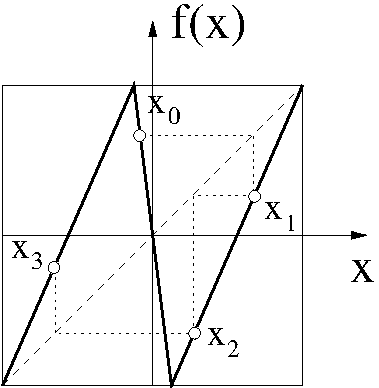
\includegraphics[width=0.35\textwidth]{bimodTraj-a}
(b)~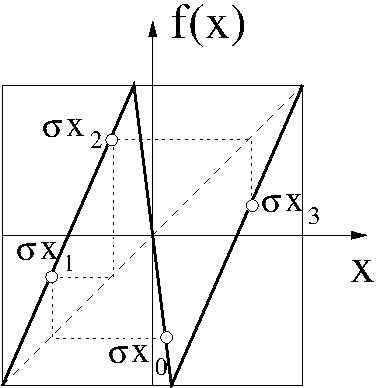
\includegraphics[width=0.35\textwidth]{bimodTraj-b}
}{}{
The bimodal Ulam sawtooth map with the $\Dn{1}$ symmetry $f(-\ssp)=-f(\ssp)$.
If the trajectory (a)
$\ssp_0 \to \ssp_1 \to \ssp_2 \to \cdots$ is a solution,
so is its reflection (b)
$\Refl\ssp_0 \to \Refl\ssp_1 \to \Refl\ssp_2 \to \cdots$.
~~(work through \refexam{exam:ReflectA};
continued in \reffig{dscr:f_1d_symm_a}).
}{dscr:f_1d_symm_A}
%%%%%%%%%%%%%%%%%%%%%%%%%%%%%%%%%%%%%%%%%%%%%%%%%%%%%%%%%%%%%%%
    %
    % finiteGrD1.mp4             length  13:11
    % Title:  Example: a 1-dimensional system with a symmetry
    % [2015-01-28 Predrag} clipped
    % re-recording and replacement for discrete1D1.mp4
    % 4:29 write "false claim - this is not a fixed point!"
\toVideo{youtube.com/embed/sI39jMdjxVM} % uploaded 2015-01-04
    %
The map is reflection-symmetric, $\map(-\ssp) = - \map(\ssp)$.

Denote the reflection operation by $\Refl\ssp = - \ssp$.
The 2-element
group $\Group=\{e,\Refl\}$ goes by many names, such as $Z_2$ or $\Cn{2}$.
Here we shall refer to it as $\Dn{1}$, dihedral group generated by a single
reflection. The $\Group$-equivariance of the map implies that if
$\{\ssp_n\}$ is a trajectory, than also $\{\Refl\ssp_n\}$ is a
symmetry-equivalent trajectory because
$
\Refl\ssp_{n+1} = \Refl f(\ssp_n) = f(\Refl \ssp_n)
\,.
$

In the temporal lattice formulation, there is a triplet of fields
\(
\field_\zeit=(\field^{L}_{\zeit},\field^{C}_{\zeit},\field^{R}_{\zeit})
\)
at each lattice site $\zeit$.
Just like the temporal Bernoulli \refeq{diffEqs:1stepDiffEq},
temporal {\lattstate}s satisfy a linear first-order difference equation
\beq
\field_{\zeit} - \map\circ\field_{\zeit-1} = 0
\,,
\ee{sawtooth:1stepDiffEq}
but now for a triplet of fields satisfying the local condition
\refeq{symmBimod} at each lattice site. As the local slope can be either
$\ExpaEig$ or $\ExpaEig_C$, the $[3\cl{}\!\times\!3\cl{}]$ {\jacobianOrb}
$\jMorb$ takes a block-diagonal form, and depends on the symbol \brick\
of a particular {\lattstate}.
\bigskip

{\color{red}Challenge}: write down the \HillDet\ for a given symbol \brick,
not only using Hill's formula, but also directly, without time evolution.

~~(continued in \refexam{exam:Reflecti})
    \PC{2021-06-12}
       {write up exercise {exer:ReflectA}: write down the formula for
        the map of \reffig{dscr:f_1d_symm_A}, verify its $\Dn{1}$-equivariance.}
                                        \jumpBack{exam:ReflectA}
} %end \example{A reflection symmetric $1d$ map:
%%%%%%%%%%%%%%%%%%%%%%%%%%%%%%%%%%%%%%%%%%%%%%%%%%%%%%%%%%%%%%%%%%

\renewcommand{\Refl}{\ensuremath{{s}}} % Dihedral wiki convention

%% A reflection symmetric $1d$ map.  % RETURN to ChaosBook
    % siminos/spatiotemp/Examples/examReflecti.tex
% $Author: predrag $ $Date: 2021-08-02 20:53:14 -0400 (Mon, 02 Aug 2021) $

\renewcommand{\Refl}{\ensuremath{{\sigma}}} % conflict with ``symmetric''

%%%%%%%%%%%%%%%%%%%%%%%%%%%%%%%%%%%%%%%%%%%%%%%%%%%%%%%%%%%%%%%%%%
\BFIG{1.0}{bimodSaw}{}{
The $\Dn{1}$-equivariant bimodal sawtooth map of
\reffig{dscr:f_1d_symm_A} has three types of
\po s:
(a) $\Dn{1}$-fixed fixed point \cycle{C},
asymmetric fixed points pair $\{\cycle{L},\cycle{R}\}$.
(b) $\Dn{1}$-symmetric ({setwise} invariant) 2-cycle \cycle{LR},
composed of the relative cycle segment from $L$ to $R$
and its repeat from $R$ to $L$.
(c) Asymmetric 2-cycles pair $\{\cycle{LC},\cycle{CR}\}$.
~~(study \refexam{exam:Reflecti};
   continued in \reffig{dscr:f_1d_symm_b})
\authorYL{}
}{dscr:f_1d_symm_a}
%%%%%%%%%%%%%%%%%%%%%%%%%%%%%%%%%%%%%%%%%%%%%%%%%%%%%%%%%%%%%%%

%%%%%%%%%%%%%%%%%%%%%%%%%%%%%%%%%%%%%%%%%%%%%%%%%%%%%%%%%%%%%%%%%%%%%%%
\example{$\Dn{1}$-asymmetric cycles.}{ \label{exam:Reflecti} % was dscr:Reflecti
% in examDiscrete.tex, called by \Chapter{discrete}{}{World in a mirror}
% was titled "Group $\Dn{1}$ - a reflection symmetric $1d$ map"
        \index{sawtooth map}\index{map!sawtooth}             \toCB
(Continued from \refexam{exam:ReflectA})~~
	% discreteD1.mp4
	% Title:     Handwritten: a 1-dimensional fundamental domain
	% "It does not say anyplace in the Bible that if equations of motion
	% have a symmetry, solutions should have it too."
	\PC{2019-02-18}{REPLACE discreteD1.mp4, eventually.}
\toVideo{youtube.com/embed/Le5LvdDWSFQ} % uploaded 2015-01-04
    %
The $\Dn{1}$-equivariance of a map, $\Dn{1}=\{e,\Refl\}$, implies that,
in particular, if
a finite set of states ${\pS}_p=\{\ssp_n\}$ constitutes a \po\ $p$, so
does its reflection ${\pS}_{\Refl{p}}=\{\Refl\ssp_n\}$, with the same
period and the same stability properties.

Label the three regions $\pS=\{\pS_L,\pS_C,\pS_R\}$ of the bimodal
`sawtooth' map of \reffig{dscr:f_1d_symm_a}, with a 3-letter alphabet
$L$(eft), $C$(enter), and $R$(ight). This symbolic dynamics is complete
ternary dynamics, with any sequence of letters $\alphabet=\{L,C,R\}$
corresponding to an \admissible\ trajectory (`complete' means no
additional grammar rules required, see \refexam{exam:compBinSymbDyn}
below).

If $\asym$  is an \emph{asymmetric} cycle $\tilde{\pS}_\asym$, $\Refl$
maps it into the reflected cycle $\Refl\tilde{\pS}_\asym$, with no points
in common, $\tilde{\pS}_\asym\cap\Refl\tilde{\pS}_\asym=\emptyset$.
Examples are the fixed points pair $\{\cycle{L},\cycle{R}\}$ and the
2-cycles pair $\{\cycle{LC},\cycle{CR}\}$ in
\reffig{dscr:f_1d_symm_a}\,(c).
                                        \jumpBack{exam:Reflecti}
        } % end \example{exam:Reflecti}
%%%%%%%%%%%%%%%%%%%%%%%%%%%%%%%%%%%%%%%%%%%%%%%%%%%%%%%%%%%%%%%%%%%%%%%

%%%%%%%%%%%%%%%%%%%%%%%%%%%%%%%%%%%%%%%%%%%%%%%%%%%%%%%%%%%%%%%%%%%%%%%
\example{$\Dn{1}$-symmetric cycles.}{ \label{exam:ReflectiSS} % was dscr:ReflectiSS
% in examDiscrete.tex, called by \Chapter{discrete}{}{World in a mirror}
        \index{sawtooth map}\index{map!sawtooth}             \toCB
(Continued from \refexam{exam:Reflecti})~~
For $\Dn{1}$  the period of a {set-wise} symmetric cycle is even ($\nsym
= 2 \nsymf$), and the mirror image of the $\ssp_\sym$ periodic point is
reached by traversing the \rpo\ segment $\symf$  of length $\nsymf$,
$\flow{\nsymf}{\ssp_\sym} = \Refl \ssp_\sym $, see
\reffig{dscr:f_1d_symm_a}\,(b).
                                        \jumpBack{exam:ReflectiSS}
        } % end \example{Reflection symmetric 1-d maps}{exam:ReflectiSS
%%%%%%%%%%%%%%%%%%%%%%%%%%%%%%%%%%%%%%%%%%%%%%%%%%%%%%%%%%%%%%%%%%%%%%%

%%%%%%%%%%%%%%%%%%%%%%%%%%%%%%%%%%%%%%%%%%%%%%%%%%%%%%%%%%%%%%%%%%%%%%%
\example{$\Dn{1}$-invariant cycles.}{ \label{exam:ReflectiPS} % was dscr:ReflectiPS
% in examDiscrete.tex, called by \Chapter{discrete}{}{World in a mirror}
        \index{sawtooth map}\index{map!sawtooth}             \toCB

\Fix{\Group}, the set of points invariant under group action of $\Dn{1}$,
$\tilde{\pS} \cap \Refl \tilde{\pS}$, is just this fixed point $\ssp=0$,
the reflection symmetry point.

In the example at hand there is only one \Group-invariant (point-wise
invariant) orbit, the fixed point \cycle{C} at the origin, see
\reffig{dscr:f_1d_symm_a}\,(a). As reflection symmetry is the only
discrete symmetry that a map of the interval can have, this example
completes the group-theoretic analysis of 1\dmn\ maps. We shall continue
analysis of this system in \refexam{dscr:C2FundDom}, and work out the
symbolic dynamics of such reflection symmetric systems in
\refexam{exam:Symm1d}).    % was (\refsect{s-C-2-fact})
                                        \jumpBack{exam:ReflectiPS}
        } % end \example{Reflection symmetric 1-d maps}{exam:ReflectiPS
%%%%%%%%%%%%%%%%%%%%%%%%%%%%%%%%%%%%%%%%%%%%%%%%%%%%%%%%%%%%%%%%%%%%%%%

%%%%%%%%%%%%%%%%%%%%%%%%%%%%%%%%%%%%%%%%%%%%%%%%%%%%%%%%%%%%%%%%%%
\FIG{
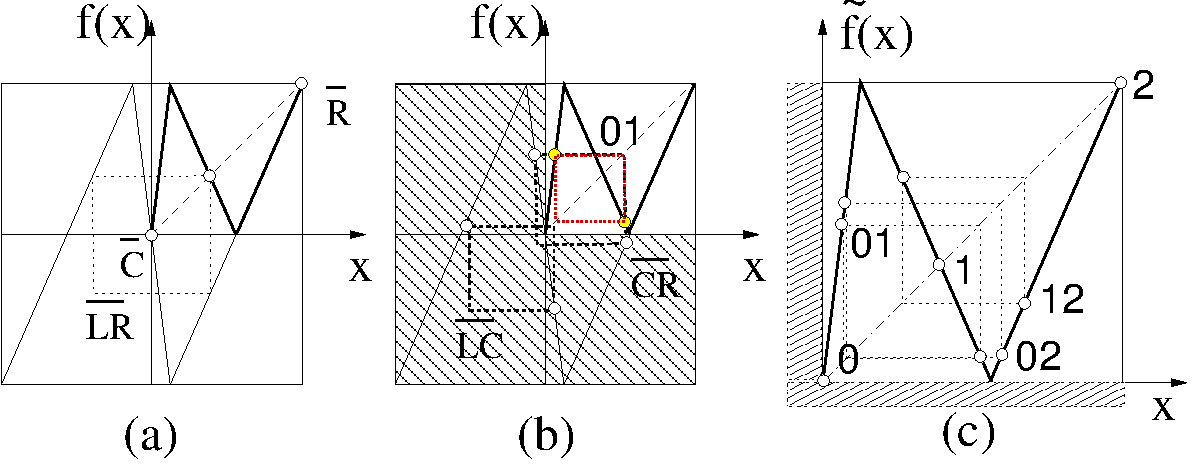
\includegraphics[width=0.95\textwidth]{bimodFund}
}{}{
The bimodal Ulam sawtooth map of \reffig{dscr:f_1d_symm_a}
with the $\Dn{1}$ symmetry $f(-\ssp)=-f(\ssp)$,
restricted to the fundamental domain.
$f(\ssp)$ is indicated by the thin line, and
fundamental domain map ${\tilde\map}({\tilde \ssp})$ by the
thick line.
(a) Boundary fixed point \cycle{C} is the fixed point \cycle{0}.
The asymmetric fixed point pair \{\cycle{L},\cycle{R}\}
is reduced to the fixed point \cycle{2},
and the full \statesp\ symmetric 2-cycle
\cycle{LR} is reduced to the fixed point \cycle{1}.
(b) The asymmetric 2-cycle pair
\{\cycle{LC},\cycle{CR}\} is reduced to 2-cycle \cycle{01}.
(c) All fundamental domain fixed points and 2-cycles.
~~(work through \refexam{dscr:C2FundDom} )
% continued in #\reffig{??}).
\authorYL{}
}{dscr:f_1d_symm_b}
%%%%%%%%%%%%%%%%%%%%%%%%%%%%%%%%%%%%%%%%%%%%%%%%%%%%%%%%%%%%%%%

%%%%%%%%%%%%%%%%%%%%%%%%%%%%%%%%%%%%%%%%%%%%%%%%%%%%%%%%%%%%%%%%%%%%%%%
\example{$\Dn{1}$ reduction to the fundamental domain.}
{ \label{dscr:C2FundDom}
% in examDiscrete.tex, called by \Chapter{discrete}{}{World in a mirror}
        \index{sawtooth map}\index{map!sawtooth}             \toCB
Consider again
the reflection-symmetric bimodal Ulam sawtooth map $f(-\ssp)=-f(\ssp)$
of \refexam{exam:Reflecti}, with symmetry group $\Dn{1}=\{{ e},\Refl\}$.
The {\statesp} $\pS = [-1,1]$
can be tiled by half-line $\tilde{\pS}=[0,1]$, and
${ \Refl}\tilde{\pS}=[-1,0]$, its image under
a reflection across $\ssp=0$ point.
The dynamics can then be restricted to the
{\em fundamental domain} $\tilde{\ssp}_k \in \tilde{\pS}=[0,1]$;
every time a trajectory leaves this interval, it is
mapped back using $\Refl$.

In \reffig{dscr:f_1d_symm_b}
% the bimodal Ulam sawtooth map
% $f(\ssp)$ is indicated by the thin line.
the fundamental
domain map ${\tilde\map}({\tilde \ssp})$
% , indicated by the thick line, %in \reffig{dscr:f_1d_symm_b},
is obtained by reflecting $\ssp < 0$ segments
of the global map $f(\ssp)$ %, \reffig{dscr:f_1d_symm_a}\,(a),
into the upper right quadrant.
${\tilde\map}$ is also bimodal and piecewise-linear,
with $\tilde{\pS} = [0,1]$ split into three regions
$\tilde{\pS} = \{\tilde{\pS}_0,\tilde{\pS}_1,\tilde{\pS}_2\}$
which we label with a 3-letter alphabet
$\tilde{\alphabet} = \{0,1,2\}$.
The symbolic dynamics is
again complete ternary dynamics, with any sequence of
letters $\{0,1,2\}$ \admissible.

However, the interpretation of the `desymmetrized'
dynamics is quite different - the multiplicity of
every \po\ is now 1, and {relative periodic segments}
of the full \statesp\ dynamics
are all \po s in the fundamental domain.
Consider \reffig{dscr:f_1d_symm_b}:

In (a)
the boundary fixed point \cycle{C} is also the fixed point \cycle{0}.
%
The asymmetric fixed point pair \{\cycle{L},\cycle{R}\}
is reduced to the fixed point \cycle{2},
and the full \statesp\ symmetric 2-cycle
\cycle{LR} is reduced to the fixed point \cycle{1}.
(b) The asymmetric 2-cycle pair
\{\cycle{LC},\cycle{CR}\} is reduced to the 2-cycle \cycle{01}.
Finally, the symmetric 4-cycle
\cycle{LCRC} is reduced to the 2-cycle \cycle{02}.
This completes the conversion from the full \statesp\ for all
fundamental domain fixed points and 2-cycles,
frame~(c).
	\PC{2019-02-18}{draw this cycle both in the full and in the
            fundamental domain.
		\\
	    in \reffig{dscr:f_1d_symm_b}\,(a) double label,
		with \cycle{0}, \cycle{1} and \cycle{2}.}
                                        \jumpBack{dscr:C2FundDom}
    } %end \example{Group $\Dn{1}$ - fundamental domain}
%%%%%%%%%%%%%%%%%%%%%%%%%%%%%%%%%%%%%%%%%%%%%%%%%%%%%%%%%%%%%%%%%%%%%%%

\renewcommand{\Refl}{\ensuremath{{s}}} % Dihedral wiki convention

%% \Dn{1}-reduced symbolic dynamics: % RETURN to ChaosBook
    % siminos/spatiotemp/Examples/examSymm1d.tex
% $Author: predrag $ $Date: 2021-08-25 23:18:52 -0400 (Wed, 25 Aug 2021) $

\renewcommand{\Refl}{\ensuremath{{\sigma}}} % conflict with ``symmetric''

%%%%%%%%%%%%%%%%%%%%%%%%%%%%%%%%%%%%%%%%%%%%%%%%%%%%%%%%%%%%%%%
\FIG{
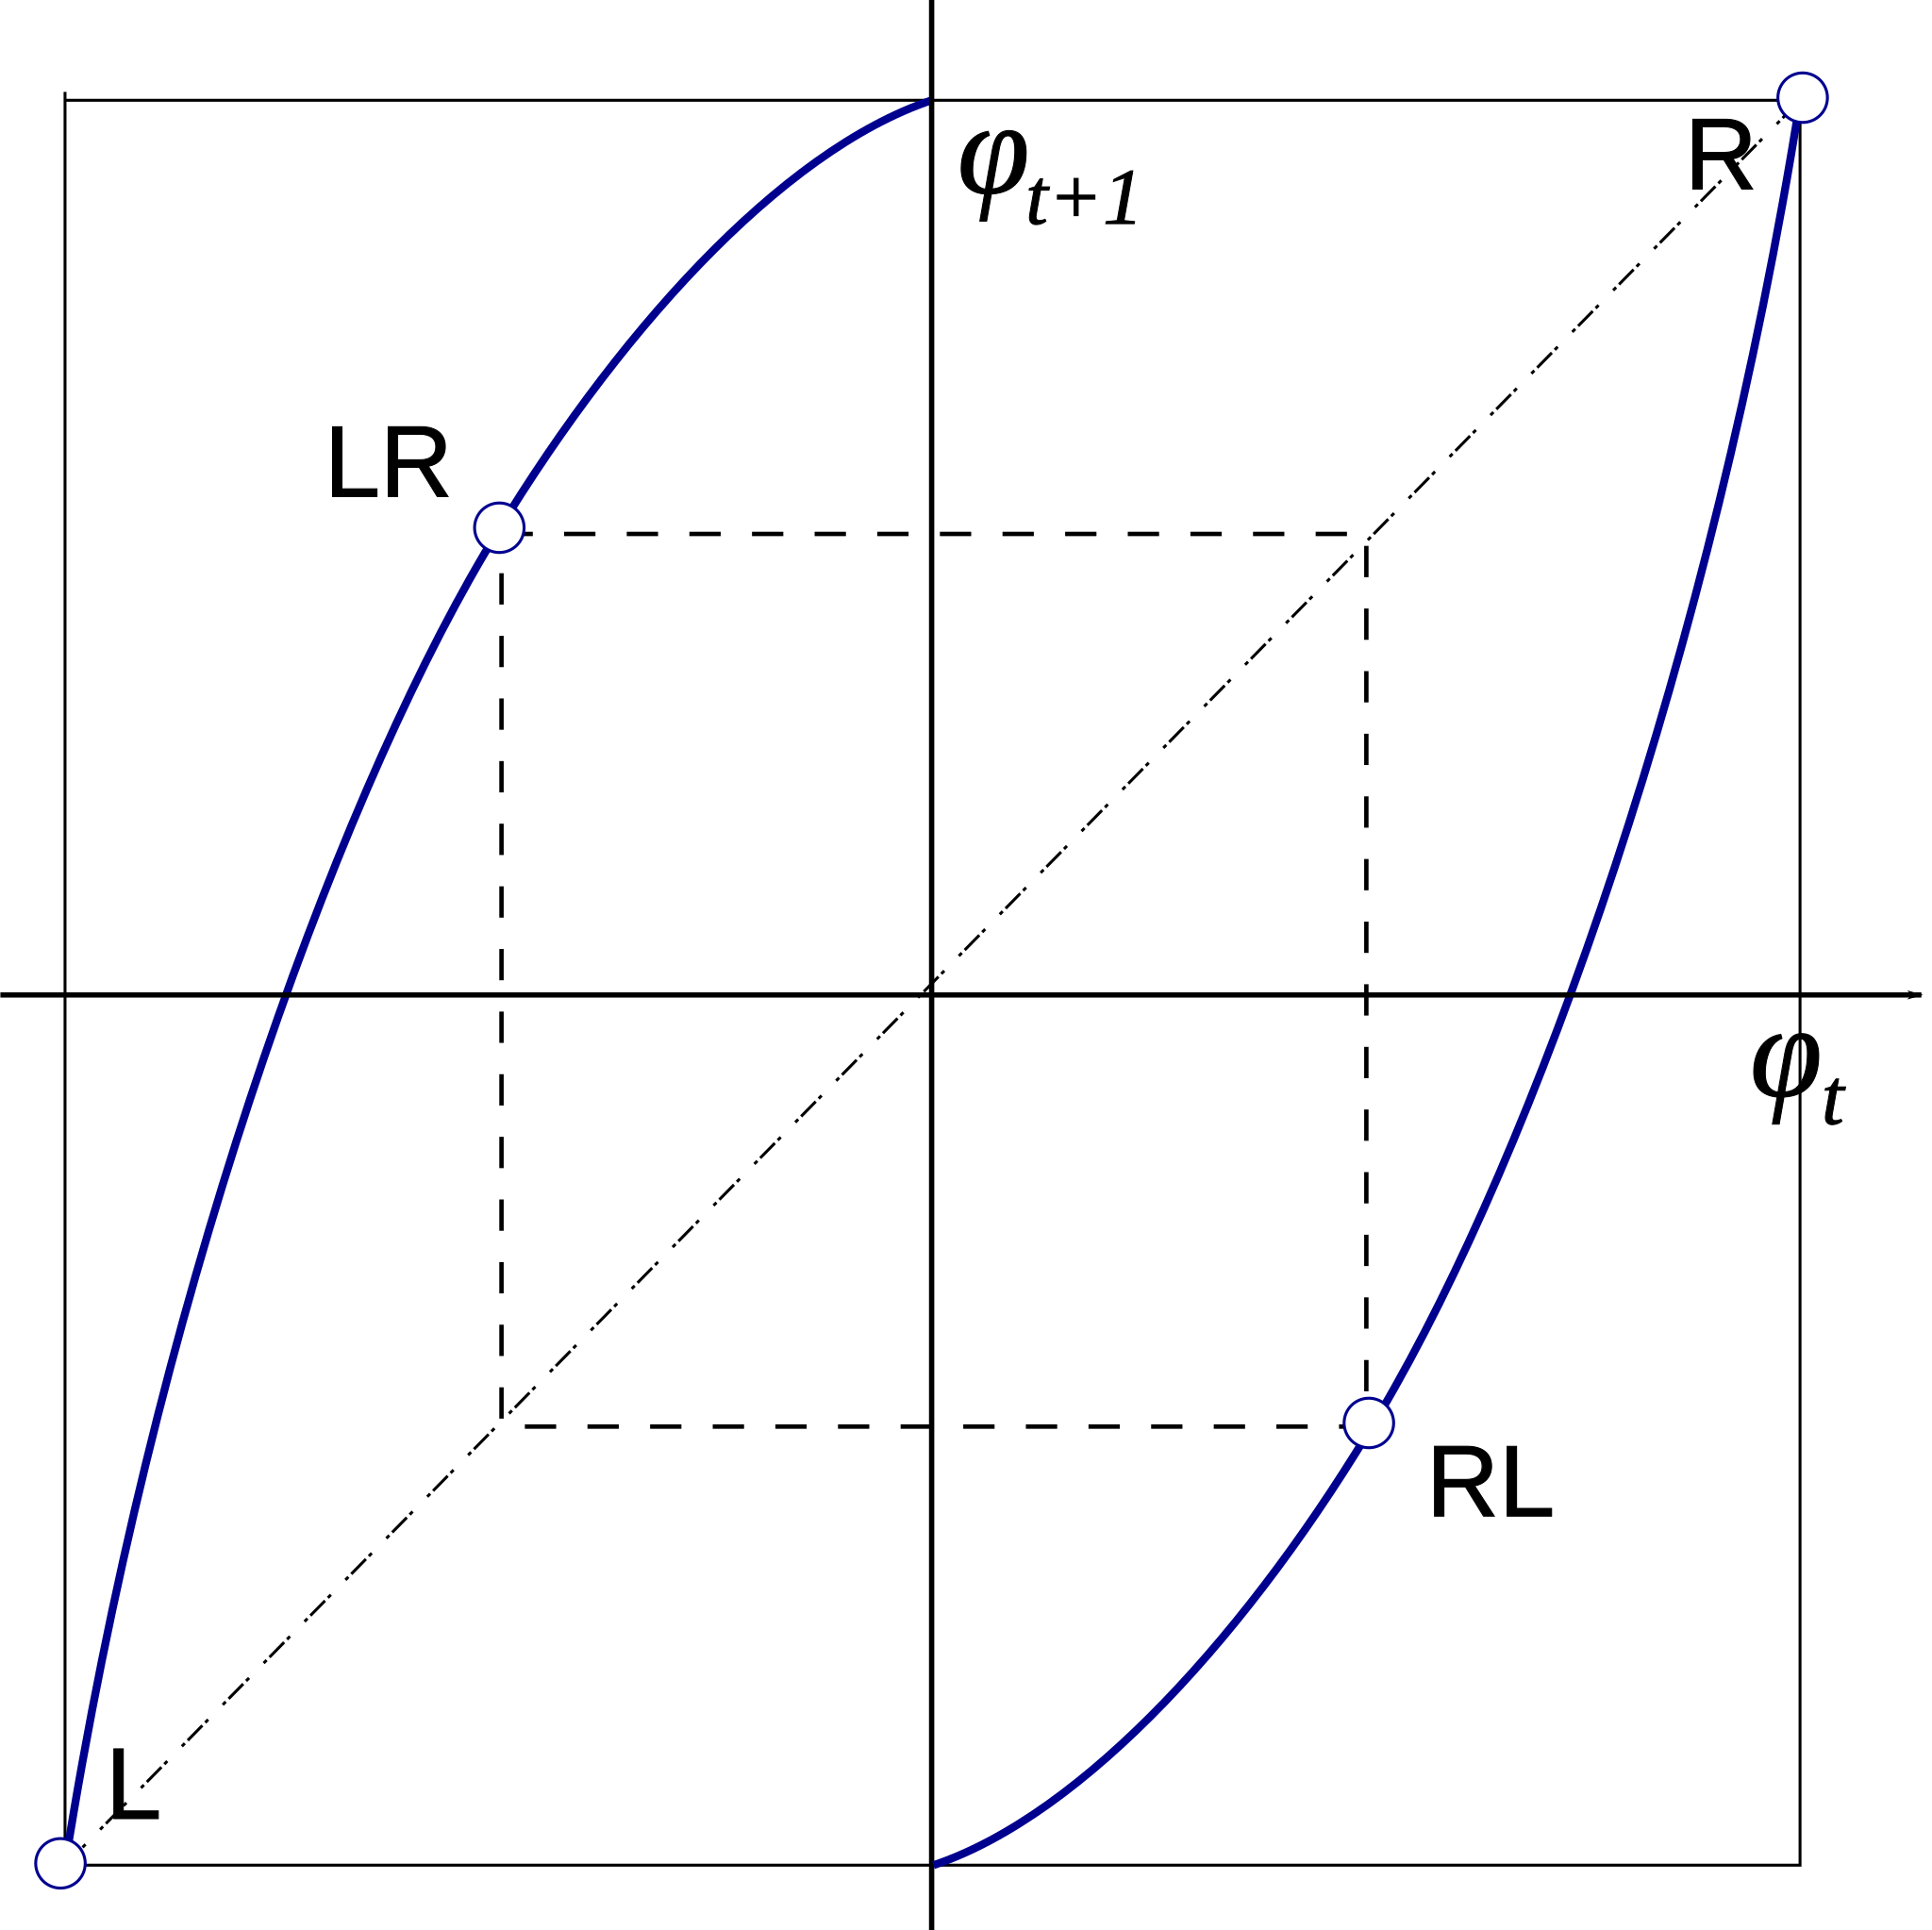
\includegraphics[width=0.35\textwidth]{BernBent}
}{}{
The $\Dn{1}$-equivariant `bent Bernoulli' map has two types of
\po s:
(a)
asymmetric pairs, such as the fixed points pair $\{\cycle{L},\cycle{R}\}$.
(b) $\Dn{1}$-symmetric ({setwise} invariant) \po s, such as the 2-cycle \cycle{LR},
composed of the relative cycle segment from $L$ to $R$
and its repeat from $R$ to $L$.
~~(study \refexam{exam:Symm1d};
   continued in \reffig{Symm1d:BernBentFund})
}{Symm1d:BernBent}
%%%%%%%%%%%%%%%%%%%%%%%%%%%%%%%%%%%%%%%%%%%%%%%%%%%%%%%%%%%%%%%

%%%%%%%%%%%%%%%%%%%%%%%%%%%%%%%%%%%%%%%%%%%%%%%%%%%%%%%%%%%%%%%%%%
\FIG{
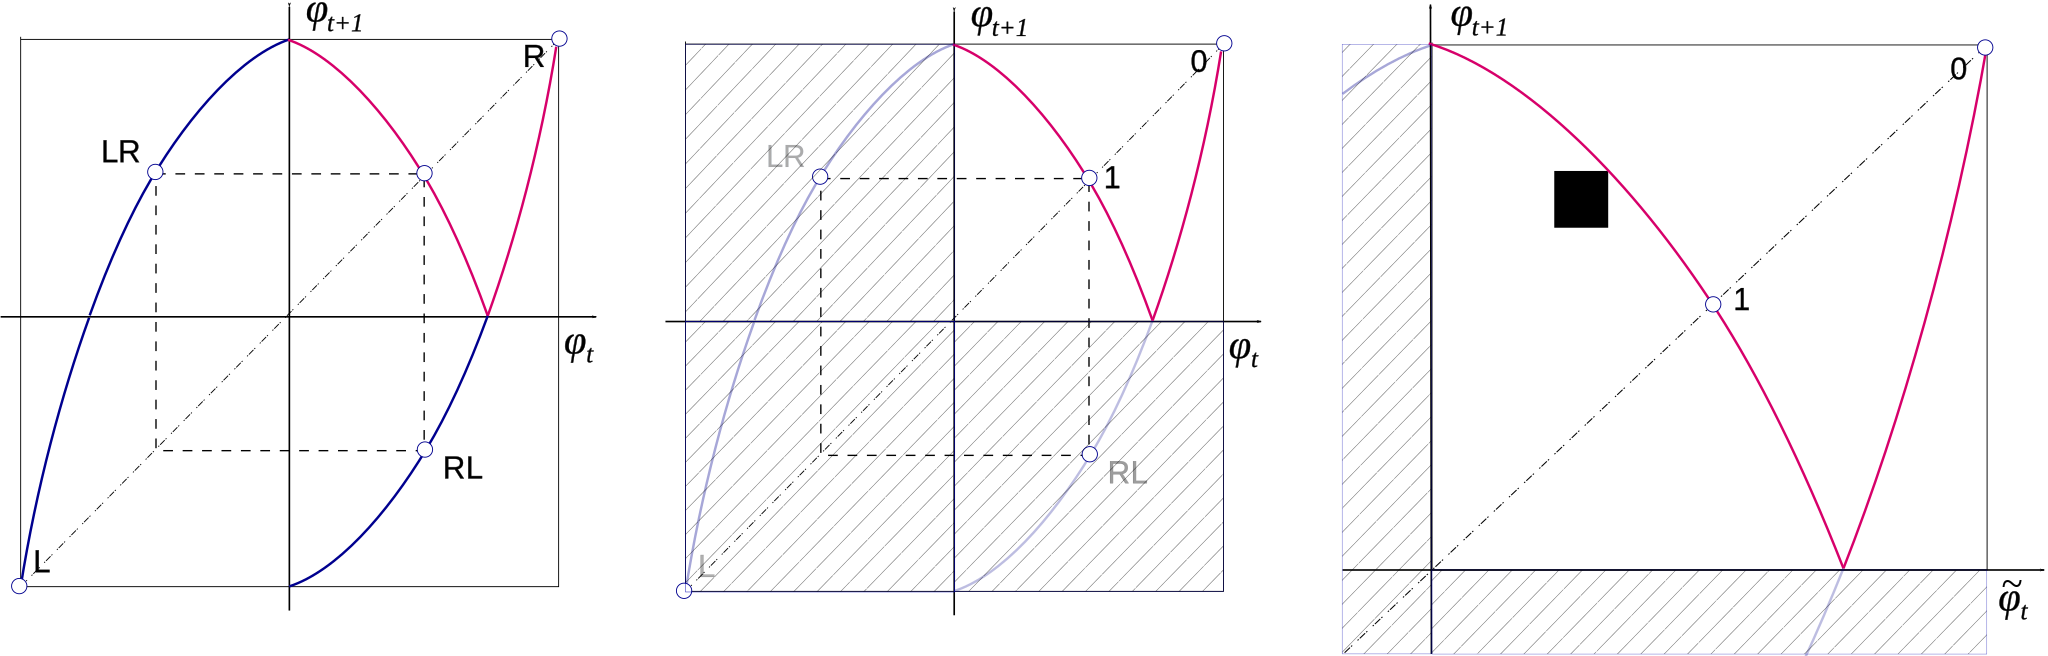
\includegraphics[width=0.80\textwidth]{BernBentFund}
}{}{
The `bent Bernoulli' map of \reffig{Symm1d:BernBent}
with the $\Dn{1}$ symmetry $f(-\field)=-f(\field)$, restricted to the
fundamental domain. $f(\field)$ is indicated by a blue line, and
fundamental domain map ${\tilde\map}({\tilde \field})$ by the purple line.
The asymmetric fixed point pair \{\cycle{L},\cycle{R}\} is reduced to the
fixed point \cycle{0}, and the full \statesp\ symmetric 2-cycle
\cycle{LR} is reduced to the fixed point \cycle{1}.
~~(work through \refexam{exam:Symm1d})
% continued in #\reffig{??}).
}{Symm1d:BernBentFund}
%%%%%%%%%%%%%%%%%%%%%%%%%%%%%%%%%%%%%%%%%%%%%%%%%%%%%%%%%%%%%%%

%%%%%%%%%%%%%%%%%%%%%%%%%%%%%%%%%%%%%%%%%%%%%%%%%%%%%%%%%%%%%%%
% from \2020-12-18 Chapter{smale}{16jan2014}{Stretch, fold, prune}
%Table 4
\begin{table}
\caption[]{\small Correspondence between the $\Dn{1}$ symmetry
reduced cycles $\tilde{p}$ and the full \statesp\
periodic orbits ${p}$, together with their
multiplicities $m_p$. Also listed are the two shortest cycles
(length 6) related by time reversal, but distinct under $\Dn{1}$.
}
{\small
\begin{tabular}{lll}
%\hline
$\tilde{p}$ & ${p}$  & $m_p$ \\
\hline
 0  & $R$ & 2 \\
 1 & $LR$ & 1 \\ %\hline
 01 & $LLRR$   & 1 \\ %\hline
 011 & $LLR$  & 2 \\
 001 & $LLLRRR$ & 1 \\
%\hline
 0111 & $LRLLRLRR$  & 1 \\
 0001 & $LRRR$ & 2 \\
 0011 & $LLLLRRRR$ & 1 \\
%\hline
 01111 & $LRLRL$ & 2 \\
 00111 & $LRLLLRLRRR$  & $1$ \\
 11010 & $LRRLLRLLRR$ & $1$ \\
 00011 & $LRLLLRLRRR$   &    $1$ \\
 10100 & $LLRRR$   &    $2$ \\
 00001 & $LLLLLRRRRR$ & $1$ \\
%\hline
 110100 & $LRRLLLRLLRRR$ & $1$ \\
 110010 & $LRRRLLRLLLRR$ & $1$ %\\
%\hline
\end{tabular}
} %end \small
\label{dscr:t-symm-4}
\end{table}
%%%%%%%%%%%%%%%%%%%%%%%%%%%%%%%%%%%%%%%%%%%%%%%%%%%%%%%%%%%%%%%

%%%%%%%%%%%%%%%%%%%%%%%%%%%%%%%%%%%%%%%%%%%%%%%%%%%%%%%%%%%%%%%%%%%%%%%
\example{\Dn{1}-reduced binary symbolic dynamics.}{  \label{exam:Symm1d}
% was \section{$\Zn{2} = \Dn{1}$ factorization}
% was \label{s-C-2-fact} in ChaosBook - REPLACE!
% was section siminos/spatiotemp/chapter/symm1d.tex
% Predrag                               20sep2017
% extracted from symm.tex {Discrete symmetry factorization}
% Predrag                                7apr2015
\index{dihedral group!\Dn{1}}
\index{group!\Dn{1}}                                    \toCB

    \PC{2017-09-20}{
Extracted this %\refsect{s-C-2-fact}
from ChaosBook \texttt{symm.tex} {\em Discrete symmetry factorization},
\toChaosBook{section.25.5}
{sect.~25.5} {\em $\Zn{2} = \Dn{1}$ factorization}
(version of 2015-04-07).
    }
%    \PC{2021-08-01}{
% Drew a bent Bernoulli map; like Bernoulli, but the two branches are curved}
%
Consider a nonlinear, $\Dn{1}$-symmetric `bent Bernoulli' map  of
\reffig{Symm1d:BernBent}; like the bimodal map \reffig{dscr:f_1d_symm_a},
but with the middle interval squeezed to a point, so the symbolic
dynamics is simpler, complete binary with  a 2-letter alphabet $L$(eft),
$R$(ight).

In \reffig{Symm1d:BernBentFund} the fundamental domain map
${\tilde\map}({\tilde\field})$ is obtained by reflecting $\field < 0$
segments of the global map $f(\field)$ into the upper right quadrant.
${\tilde\map}$ also has two branches, with $\tilde{\pS} = [0,1]$ split
into two regions $\tilde{\pS} = \{\tilde{\pS}_0,\tilde{\pS}_1\}$ which we
label with a 2-letter alphabet $\tilde{\alphabet} = \{0,1\}$. While the
full \statesp\ map has two monotone branches with positive slopes, the
symmetry reduced map is a unimodal map, with negative slope branch
$\tilde\map_1$.

The negative slope branch is the consequence of relative periodicity: the
mirror image of the $\ssp_\sym$ periodic point is reached by traversing
the \rpo\ segment $\symf$  of length $\nsymf$, $\flow{\nsymf}{\ssp_\sym}
= \Refl \ssp_\sym $, see the $LR$ 2-cycle in \reffig{Symm1d:BernBent}, so
the \rpo\ temporal {\JacobianM} carries a minus sign.

We could have illustrated this with the Bernoulli piecewise linear map,
\reffig{fig:BernPart}, whose symmetry-reduced map is the Ulam tent map,
but there the \Dn{1} symmetry is so obvious that it is hidden in the
plain sight.
       \PC{2021-08-03}{
Make up the Bernoulli \Dn{1}-symmetry example, setting up
\refexam{exam:BernD1zeta}, will need it for \textbf{LC21}.
        }

The symbolic dynamics is again complete binary dynamics, with any
sequence of letters $\{0,1\}$ \admissible.
Assume that all \po s are strictly unstable, $|\ExpaEig_p>0|$,  so that
each orbit or orbit is uniquely labeled by an infinite string
$\{\Ssym{i}\}$, $\Ssym{i}\in\{R,L\}$, and that the dynamics is invariant
under the $ R \leftrightarrow L $ interchange, \ie, it is $\Dn{1}$
symmetric. The \po s separate into the symmetric orbits
\(
\sym\in\{RL, RRLL, RRRLLL, RLLRLRRL, \cdots\}
\,,
\)
with multiplicity $m_\sym=1$, and the asymmetric orbit pairs
\(
\asym\in\{R, L, RRL, LLR, \cdots\}
\,,
\)
with multiplicity $m_\asym=2$. For example, as there is no
distinction between % the ``up" and the ``down" spins, or
the ``left" or the ``right" branch of the map, the weights
$t_R=t_L$,  $t_{RRL}=t_{RLL}$, are equal, and so on.
\exerbox{e_Lor_Ising}

The symmetry reduced labeling $\symf_i \in \{0,1\}$ is related to the full
\statesp\ labels $\Ssym{i} \in \{L,R\}$ % L(eft), R(ight) % was Ising spin
by
\bea
\mbox{If} \quad \Ssym{i} & = & \Ssym{i-1} \quad \mbox{then} \quad \symf_i=0
     \continue
\mbox{If} \quad \Ssym{i} & \neq & \Ssym{i-1} \quad \mbox{then} \quad \symf_i=1
\eea
For example, both $\cycle{L}=\cdots{LLLL}\cdots$ and
$\cycle{R}=\cdots{RRRR}\cdots$ map into $\cdots{000}\cdots=\cycle{0}$,
$\cycle{LR}=\cdots{LRLR}\cdots$ maps into $\cdots{111}\cdots=\cycle{1}$,
$\cycle{LRRL}=\cdots{LLRRLLRR}\cdots$
maps into $\cdots{0101}\cdots = \cycle{01}$, and so forth.
A list of such reductions is given in  \reftab{dscr:t-symm-4}.
   \PC{2021-08-02}{
    please recheck \reftab{dscr:t-symm-4}: I have interchanged `0' and
    `1' compared to ChaosBook, might have introduced errors.}
%
~~(continued in \refexam{exam:Fact1d},
   illustrated by the Bernoulli \refexam{exam:BernD1zeta})
\index{Ising model}
                                        \jumpBack{exam:Symm1d}
    } %end \example{exam:Symm1d}
%%%%%%%%%%%%%%%%%%%%%%%%%%%%%%%%%%%%%%%%%%%%%%%%%%%%%%%%%%%%%%%%%%%%%%%

\renewcommand{\Refl}{\ensuremath{{s}}} % Dihedral wiki convention



%%%%%%%%%%%%%%%%%%%%%%%%%%%%%%%%%%%%%%%%%%%%%%%%%%%%%%%%%%%%%%%%%%%%%%
%% 2021-07-23 from Xiong's siminos/xiong/thesis/chapters/symGroup.tex
%% XXX.
    % siminos/spatiotemp/Examples/examC3matrRep.tex
% $Author: predrag $ $Date: 2021-07-24 23:53:43 -0400 (Sat, 24 Jul 2021) $

%%%%%%%%%%%%%%%%%%%%%%%%%%%%%%%%%%%%%%%%%%%%%%%%%%%%%%%%%%%%%%%%%%%%%%
\example{A matrix representation of cyclic group $\Cn{3}$.}{
  \label{exam:C3matrRep}                                    \toCB
%% 2021-07-23 from Xiong's siminos/xiong/thesis/chapters/symGroup.tex
  A 3\dmn\ matrix representation of the 3-element cyclic group
  $\Cn{3}=\{e,\shift,\shift^2\}$ is given by the three rotations by
  $2\pi/3$ around the $z$-axis in a 3\dmn\ \statesp,
  \bea
  {D}(e) &=&
  \begin{bmatrix}
    1 & & \\
    & 1 & \\
    & & 1
  \end{bmatrix}
  \,,\quad
  {D}(\shift) =
  \begin{bmatrix}
    \cos\frac{2\pi}{3}  & -\sin\frac{2\pi}{3} & \\
    \sin\frac{2\pi}{3}  & ~\cos\frac{2\pi}{3}  & \\
    & & 1
  \end{bmatrix}
  \,,
  \continue
  {D}(\shift^2) &=&
  \begin{bmatrix}
    \cos\frac{4\pi}{3}  & -\sin\frac{4\pi}{3}  & \\
    \sin\frac{4\pi}{3}  & ~\cos\frac{4\pi}{3}  & \\
    & & 1
  \end{bmatrix}
  \,.
  \nnu
  \eea
  %\index{matrix rep!cyclic group}
  ~~(continued in \refexam{exam:C3regularRep})
                                        \jumpBack{exam:C3matrRep}
\authorXD{}
} % end {exam:C3matrRep}
%%%%%%%%%%%%%%%%%%%%%%%%%%%%%%%%%%%%%%%%%%%%%%%%%%%%%%%%%%%%%%%%%%%%%%

%% XXX.
    % siminos/spatiotemp/Examples/examC3regularRep.tex
% $Author: predrag $ $Date: 2021-07-28 17:52:52 -0400 (Wed, 28 Jul 2021) $

%%%%%%%%%%%%%%%%%%%%%%%%%%%%%%%%%%%%%%%%%%%%%%%%%%%%%%%%%%%%%%%%%%%%%%%
\begin{table}[h]
  \caption[ The multiplication tables of the $\Dn{1}$ and $\Cn{3}$]{
    The multiplication tables of the
    dihedral group $\Dn{1}$, and
    cyclic group $\Cn{3}$.
  }
  \label{tab:C3MultTab}
  \begin{center}
    \centering
    \begin{tabular}{c | c c}
      $\Dn{1}$         & $e$        & $\Refl$  \\ \hline
      $e$              & $e$        & $\Refl$   \\
      $\Refl$ & $\Refl$  & $e$         \\
    \end{tabular}
    \qquad\qquad
    \begin{tabular}{c | c c c}
      $\Cn{3}$         & $e$        & $\shift^{-1}$ & $\shift^{-2}$ \\ \hline
      $e$              & $e$        & $\shift^2$ & $\shift$  \\
      $\shift$ & $\shift$  & $e$       & $\shift^2$   \\
      $\shift^2$ & $\shift^2$  & $\shift$ & $e$
    \end{tabular}
  \end{center}
\end{table}
%%%%%%%%%%%%%%%%%%%%%%%%%%%%%%%%%%%%%%%%%%%%%%%%%%%%%%%%%%%%%%%%%%%%%%%

%%%%%%%%%%%%%%%%%%%%%%%%%%%%%%%%%%%%%%%%%%%%%%%%%%%%%%%%%%%%%%%%%%%%%%
\example{The regular representation of cyclic group $\Cn{3}$.}{
%% 2021-07-23 from Xiong's siminos/xiong/thesis/chapters/symGroup.tex
  \label{exam:C3regularRep}                                    \toCB
  \index{regular rep!cyclic group}
 (continued from \refexam{exam:C3matrRep})~~
  Take an arbitrary function $\rho(\ssp)$ over the \statesp\ $\ssp \in \pS$, and
  define a fundamental domain $\pSRed$ as a 1/3 wedge, with axis $z$ as its
  (symmetry invariant) edge. The \statesp\ is tiled with three copies of the wedge,
  \[
    \pS =  \pSRed_1\cup\pSRed_2\cup\pSRed_3
    =  \pSRed\cup \shift\pSRed\cup \shift^2\pSRed
    \,.
  \]
  Function $\rho(\ssp)$ can be written as the 3\dmn\ vector of functions
  over the fundamental domain $\sspRed \in \pSRed$,
  \beq
  (\rho_1^{reg}(\sspRed),\rho_2^{reg}(\sspRed),\rho_3^{reg}(\sspRed))
  = (\rho(\sspRed),\rho(\shift\sspRed),\rho(\shift^2\sspRed))
  \,.
  \ee{eq:C3RegRep}
  The multiplication table of $\Cn{3}$ is given in \reftab{tab:C3MultTab}.
  By \refeq{eq:RegRep}, the regular representation matrices
  $D^{reg}(\LieEl)$ have `1' at the location of $\LieEl^{-1}$ in the
  multiplication table, `0' elsewhere. The actions of the operator
  $U(\LieEl)$ are now represented by permutations matrices (blank entries
  are zeros):
  \beq
  D^{reg}(e) = %&=&
  \begin{bmatrix}
    1 & & \\
    & 1 & \\
    & & 1 \\
  \end{bmatrix} \,,  \quad
  % \continue
  D^{reg}(\shift) = %&=&
  \begin{bmatrix}
    ~ & 1 & ~\\
    ~ & ~ & 1\\
    1 & ~ & ~ \\
  \end{bmatrix}\,,  \quad
  D^{reg}(\shift^2) =
  \begin{bmatrix}
    ~ & ~ & 1\\
    1 & ~ & ~\\
    ~ & 1 & ~ \\
  \end{bmatrix}
  \,.
  \label{eq:C3reg}
  \eeq
                                        \jumpBack{exam:C3regularRep}
\authorXD{}
} %end \example{exam:C3regularRep}
%%%%%%%%%%%%%%%%%%%%%%%%%%%%%%%%%%%%%%%%%%%%%%%%%%%%%%%%%%%%%%%%%%%%%%

%% XXX.
    % siminos/spatiotemp/Examples/examC3irReps.tex
% $Author: predrag $ $Date: 2021-07-28 17:52:52 -0400 (Wed, 28 Jul 2021) $

%%%%%%%%%%%%%%%%%%%%%%%%%%%%%%%%%%%%%%%%%%%%%%%%%%%%%%%%%%%%%%%%%%%%%%
\example{Irreps of cyclic group $\Cn{3}$.}{
  \label{exam:C3irReps}                                     \toCB
%% 2021-07-23 from Xiong's siminos/xiong/thesis/chapters/symGroup.tex
  (continued from \refexam{exam:C3regularRep})~~
  For $\Dn{1}$, whose multiplication table is in \reftab{tab:C3MultTab}, we can form
  the symmetric base $\rho(\sspRed) + \rho(\Refl\sspRed)$
  and the antisymmetric base $\rho(\sspRed) - \rho(\Refl\sspRed)$. You can verify
  that in this new basis, $\Dn{1}$ is block-diagonalized.
  We would like to generalize this symmetric-antisymmetric
  decomposition to the order 3 group $\Cn{3}$. Symmetrization
  can be carried out on any number of functions, but there is no obvious
  anti-symmetrization. We draw instead inspiration from the Fourier
  transformation for a finite periodic lattice, and construct from the
  regular basis \refeq{eq:C3RegRep} a new set of bases
  \bea
  \rho^{irr}_0(\sspRed) &=& \frac{1}{3}\left[
    \rho(\sspRed) ~+~ \rho(\shift \sspRed) ~+~ \rho(\shift^2 \sspRed)
  \right]
  \label{eq:c3f1}\\
  \rho_1^{irr}(\sspRed) &=& \frac{1}{3}\left[
    \rho(\sspRed) + \omega\,\rho(\shift \sspRed) + \omega^2 \rho(\shift^2 \sspRed)
  \right]
  \label{eq:c3f2}\\
  \rho_2^{irr}(\sspRed) &=& \frac{1}{3}\left[
    \rho(\sspRed) + \omega^2 \rho(\shift \sspRed) + \omega\,\rho(\shift^2 \sspRed)
  \right]
  \label{eq:c3f2}
  \,.
  \eea
  Here $\omega = e^{2i\pi/3}$.
  The representation of group $\Cn{3}$ in this new basis is block-diagonal
  by inspection:
  \begin{equation}
    D^{irr}(e) =
    \begin{bmatrix}
      1 & & \\
      & 1 & \\
      & & 1 \\
    \end{bmatrix} \,,\quad
    D^{irr}(\shift) =
    \begin{bmatrix}
      1 & 0 & 0\\
      0 & \omega & 0\\
      0 & 0 & \omega^2 \\
    \end{bmatrix}  \,,\quad
    D^{irr}(\shift^2) =
    \begin{bmatrix}
      1 & 0 & 0\\
      0 & \omega^2 & 0\\
      0 & 0 & \omega \\
    \end{bmatrix}
    \,.
    \label{eq:c3irr}
  \end{equation}
  So $\Cn{3}$ has three 1\dmn\ irreps. Generalization to any
  $\Cn{n}$ is immediate: this is just a finite lattice, discrete Fourier transform.
                                        \jumpBack{exam:C3irReps}
\authorXD{}
}% end \example{examC3irReps}
%%%%%%%%%%%%%%%%%%%%%%%%%%%%%%%%%%%%%%%%%%%%%%%%%%%%%%%%%%%%%%%%%%%%%%

%% \Cn{\infty} group.
    % siminos/spatiotemp/Examples/examCinfty.tex
% $Author: predrag $ $Date: 2021-08-16 00:27:24 -0400 (Mon, 16 Aug 2021) $

%%%%%%%%%%%%%%%%%%%%%%%%%%%%%%%%%%%%%%%%%%%%%%%%%%%%%%%%%%%%%
\example{\Cn{\infty} group.}{ \label{exam:examCinfty}
                                      \toCB
Consider the integer lattice $\integers$. The \emph{infinite cyclic
group} $\Cn{\infty}$ is generated by  $\shift$, the right shift by one
lattice spacing
%(note - no inverse $r^{-1}$, so not really a group)
\beq
\Cn{\infty} = \left\langle \shift \mid
            \shift^\ell, \ell\in\integers
              \right\rangle
\,.
\ee{Cinfty}
Every finite index subgroup of the {infinite cyclic group} $\Cn{\infty}$
is also {cyclic}, isomorphic to $\Cn{\cl{}}$
\beq
H(\cl{}) = \langle  \shift^\cl{} \rangle \, ,
\ee{ArtMaz1}
with index
\beq
|\Cn{\infty}/H(\cl{})| =  |\cl{}|
\,.
\ee{ArtMaz3}


The \emph{infinite cyclic group} elements
are all shifts
\bea
\Cn{\infty}
  &=&
              \left\langle
      \shift_j
              \mid
      \shift_j= \shift^{j};\;
      j\in\integers
              \right\rangle
  \continue
  &=&
            \{
\cdots, \shift_{-2}, \shift_{-1},
        1,
        \shift_{1}, \shift_{2}, \shift_{3}, \cdots
             \}
\,,
\label{examC_infty}
\eea
where $\shift_{j}=\shift^j$ denotes translation by $j$ lattice sites.
$\shift_{0}=1$ denotes the identity.
Cyclic group multiplication adds translations.
                                      \jumpBack{exam:examCinfty}
    } %end \example{examCinfty}
%%%%%%%%%%%%%%%%%%%%%%%%%%%%%%%%%%%%%%%%%%%%%%%%%%%%%%%%%%%%%%%%%

%% Marching forward in time: Artin-Mazur zeta function.
    % siminos/spatiotemp/Examples/examArtMaz.tex
% $Author: predrag $ $Date: 2021-08-17 22:42:20 -0400 (Tue, 17 Aug 2021) $

%%%%%%%%%%%%%%%%%%%%%%%%%%%%%%%%%%%%%%%%%%%%%%%%%%%%%%%%%%%%%
\example{Marching forward in time: Artin-Mazur zeta func\-tion.}{ \label{exam:ArtMaz}
Consider the integer lattice $\integers$, invariant under infinite cyclic
group shifts by one or integer number of lattice spacings (see
\refexam{exam:examCinfty}):
\beq
\Cn{\infty} = \left\langle \shift \mid
            \shift^\ell, \ell\in\integers
              \right\rangle
\,.
\ee{Cinfty}
Every period~$\cl{}$ sublattice is $\cl{}$-steps {infinite cyclic group},
\beq
H(\cl{}) = \langle  \shift^\cl{} \rangle \, ,
\ee{ArtMaz1}
with the quotient $\Cn{\infty}/H(\cl{})$ isomorphic to $\Cn{\cl{}}$,
with multiplicity
\beq
|\Cn{\infty}/H(\cl{})| =  |\cl{}|
\,.
\ee{ArtMaz3}

Let $N_{\cl{}}$
denote the number of points in $\pS$ fixed by $\map^\cl{}$:
\beq
N_{\cl{}} = |\{\ssp \in \pS :
            \map^\cl{} (\ssp) = \ssp\}|
\,.
\ee{ArtMaz4}
The corresponding Lind zeta function \refeq{Ryu17eq:1.3} is known as the {\em
Artin-Mazur} zeta func\-tion\rf{ArtMaz65,CBcount}
\beq
\zetatop(t)
 = \exp \left(-\sum_{\cl{}=1}^\infty
\frac{t^\cl{}}{\cl{}} N_\cl{}
         \right)
\ee{ArtMaz5}  % was {Ryu17eq:2.1A}
                                        \jumpBack{exam:ArtMaz}
    } % end \example{exam:ArtMaz}
%%%%%%%%%%%%%%%%%%%%%%%%%%%%%%%%%%%%%%%%%%%%%%%%%%%%%%%%%%%%%

%% \Dn{\infty} group multiplication table.
    % siminos/spatiotemp/Examples/examDinftyMultTab.tex
% $Author: predrag $ $Date: 2021-10-13 18:02:53 -0400 (Wed, 13 Oct 2021) $

%%%%%%%%%%%%%%%%%%%%%%%%%%%%%%%%%%%%%%%%%%%%%%%%%%%%%%%%%%%%%%%%%%
\begin{table}
\caption{
\Cn{\infty} cyclic group multiplication adds up translations.
\Dn{\infty} dihedral group multiplication
adds up translations, or translates and then
reverses their direction.
    }
\begin{center}
\begin{tabular}{c|c|}
\Cn{\infty} &$\shift_j$    \\\hline
$\shift_i$  &$\shift_{i+j}$\\\hline
\end{tabular}
    \qquad\qquad
\begin{tabular}{c|cc|}
\Dn{\infty} &$\shift_j$        &$\Refl_j$\\\hline
$\shift_i$  &$\shift_{i+j}$     &$\Refl_{j-i}$\\
$\Refl_i$   &$\Refl_{i+j}$     &$\shift_{j-i}$\\\hline
\end{tabular}
\end{center}
  \label{tab:DinftyMultTab}
\end{table}
%%%%%%%%%%%%%%%%%%%%%%%%%%%%%%%%%%%%%%%%%%%%%%%%%%%%%%%%%%%%%%%%%%

%%%%%%%%%%%%%%%%%%%%%%%%%%%%%%%%%%%%%%%%%%%%%%%%%%%%%%%%%%%%%
\example{\Dn{\infty} group multiplication table.}{ \label{exam:DinftyMultTab}
                                      \toCB
The \emph{infinite dihedral group}\rf{KiLePa03} elements
are all shifts and translate-reflections
\bea
\Dn{\infty}
  &=&
              \left\langle
      \shift_i,\Refl_j
              \mid
      \shift_i\Refl_j= \Refl_j\shift_{-i};\;
      \Refl_j^2 = 1;\; i,j\in\integers
              \right\rangle
  \continue
  &=&
            \{
\cdots, \shift_{-2},\Refl_{-2}, \shift_{-1},\Refl_{-1},
        1,\Refl,
        \shift_{1},\Refl_{1}, \shift_{2},\Refl_{2}, \cdots
             \}
\,.
\label{examD_infty}
\eea
where $\shift_{j}=\shift^j$ denotes translation by $j$ lattice sites, and
$\Refl_{j}=\Refl\shift^j$ denotes reflection across the $j$th lattice
site. $\shift_{0}=1$ denotes the identity, and by definition
$\Refl_{0}=\Refl$. Dihedral group multiplication
\reftab{tab:DinftyMultTab} adds up translations, or translates and then
reverses their direction.
                                      \jumpBack{exam:DinftyMultTab}
    } %end \example{Symmetry groups  in physics:}{ \label{exmp:multTabD3}
%%%%%%%%%%%%%%%%%%%%%%%%%%%%%%%%%%%%%%%%%%%%%%%%%%%%%%%%%%%%%%%%%

%% \\Dn{\infty} subgroups and cosets.
    % siminos/spatiotemp/Examples/examDinftyCosets.tex
% $Author: predrag $ $Date: 2021-08-10 11:56:19 -0400 (Tue, 10 Aug 2021) $

%%%%%%%%%%%%%%%%%%%%%%%%%%%%%%%%%%%%%%%%%%%%%%%%%%%%%%%%%%%%%
\example{\Dn{\infty} subgroups and cosets.}{ \label{exam:DinftyCosets}
                                       \toCB
%\item[2021-07-23 Han]
%The structure of the quotient groups $\Dn{\infty}/H(\cl{})$ and
%$\Dn{\infty}/H(\cl{},k)$:
%
$H(\cl{})$, any $\cl{}$, is a translation subgroup of
$\Dn{\infty}$ (a 1\dmn\ {Bravais sublattice} \lattice\
\refeq{1DBravaisLattice},
with a {basis} vector $\mathbf{a}$ that defines
the {Bravais cell} of length \cl{}) with group elements
$\langle\shift^n\rangle>$, or, more explicitely:
\beq
H(\cl{}) = \{ \cdots, \shift_{-2 \cl{}}, \shift_{-\cl{}},
1, \shift_{\cl{}}, \shift_{2 \cl{}}, \cdots\} \, .
\ee{H(n)subgroup}
There are a $2\cl{}$ left cosets of subgroup $H(\cl{})$ in $\Dn{\infty}$:
\bea
H(\cl{}) &=& \{ \cdots, \shift_{-2 \cl{}}, \shift_{-\cl{}},
1, \shift_{\cl{}}, \shift_{2 \cl{}}, \cdots\}
    \label{H(n)cosets}\\
\Refl H(\cl{}) &=& \{ \cdots, \Refl_{-2 \cl{}}, \Refl_{-\cl{}},
\Refl, \Refl_{\cl{}}, \Refl_{2 \cl{}}, \cdots\} \continue
\shift H(\cl{}) &=& \{ \cdots, \shift_{-2 \cl{} + 1}, \shift_{-\cl{} + 1},
\shift, \shift_{\cl{}+1}, \shift_{2 \cl{}+1}, \cdots\} \continue
\Refl_{1} H(\cl{}) &=& \{ \cdots, \Refl_{-2 \cl{} + 1}, \Refl_{-\cl{} + 1},
\Refl_{1}, \Refl_{\cl{}+1}, \Refl_{2 \cl{}+1}, \cdots\} \continue
&\vdots& \continue
\shift_{\cl{}-1} H(\cl{}) &=& \{ \cdots, \shift_{-\cl{}-1}, \shift_{-1},
\shift_{\cl{}-1}, \shift_{2\cl{}-1}, \shift_{3\cl{}-1}, \cdots\} \continue
\Refl_{\cl{}-1} H(\cl{}) &=& \{ \cdots, \Refl_{-\cl{}-1}, \Refl_{-1},
\Refl_{\cl{}-1}, \Refl_{2\cl{}-1}, \Refl_{3\cl{}-1}, \cdots\}
\,. \nnu
\eea
Using elements
\(
\{1,\Refl, \shift, \Refl_{1}, \cdots, \shift_{\cl{}-1}, \Refl_{\cl{}-1}\}
\)
as representatives of these cosets we
see that the quotient group $\Dn{\infty}/H(\cl{})$ is isomorphic to the
dihedral group $\Dn{\cl{}}$.

There are $\cl{}$ infinite dihedral $H(\cl{},k)$ subgroups  of
$\Dn{\infty}$, for any $\cl{}$, $0\leq{k}<\cl{}$
({Bravais cell} of length \cl{}, with reflection point shifted $k$ steps):
\[
H(\cl{},k) = \{
\cdots, \shift_{-2 \cl{}}, \Refl_{-2\cl{}+k}, \shift_{-\cl{}},
\Refl_{-\cl{}+k}, 1,
\Refl_{k}, \shift_{\cl{}}, \Refl_{\cl{}+k}, \shift_{2 \cl{}},
\Refl_{2\cl{}+k}, \cdots
             \}
\,.
\]

The left cosets of the subgroup $H(\cl{},k)$ in $\Dn{\infty}$ are:
    \PC{2021-07-24}{
Explain that $\Refl_{j} H(\cl{},k)$ is a rearrangement.
    }
\bea
H(\cl{},k) &=& \{ \cdots, \shift_{-2 \cl{}}, \Refl_{-2\cl{}+k}, \shift_{-\cl{}},
\Refl_{-\cl{}+k}, 1, \continue
&& \Refl_{k}, \shift_{\cl{}}, \Refl_{\cl{}+k}, \shift_{2 \cl{}},
\Refl_{2\cl{}+k}, \cdots\}
    \label{H(n,k)cosets}\\
\shift H(\cl{},k) &=& \{ \cdots, \shift_{-2 \cl{}+1}, \Refl_{-2\cl{}+k+1},
\shift_{-\cl{}+1},
\Refl_{-\cl{}+k+1}, \shift \continue
&& \Refl_{k+1}, \shift_{\cl{}+1}, \Refl_{\cl{}+k+1}, \shift_{2 \cl{}+1},
\Refl_{2\cl{}+k+1}, \cdots\} \continue
&\vdots& \continue
\shift_{\cl{}-1} H(\cl{},k) &=& \{ \cdots, \shift_{-\cl{}-1},
\Refl_{-\cl{}+k-1}, \shift_{-1},
\Refl_{k-1}, \shift_{\cl{}-1}, \continue
&& \Refl_{\cl{}+k-1}, \shift_{2\cl{}-1}, \Refl_{2\cl{}+k-1}, \shift_{3\cl{}-1},
\Refl_{3\cl{}+k-1}, \cdots\}
\,.
\nnu
\eea
Using $\{1$, $\shift, \cdots, \shift_{\cl{}-1}\}$ as representatives of
these cosets we see that the quotient group $\Dn{\infty}/H(\cl{},k)$ is
isomorphic to the cyclic group $\Cn{\cl{}}$.

%\item[2021-07-27 Han]
To show that $H(\cl{},k)$ is not a normal subgroup: using \refeq{D_nConj} we have:
$\shift_i\,\Refl_k\shift_i^{-1} = \Refl_{k-2i}$. For $i \neq \cl{}$, generally
$\Refl_{k-2i} = \shift_{2i}\Refl_{k}$ is not an element of $H(\cl{},k)$.

%\item[2021-07-27 Han]
Let $\phi(\cl{})$ be a {\lattstate} that is invariant under the action
of subgroup $H(\cl{})$:
\bea
H(\cl{}) \phi(\cl{}) = \phi(\cl{}) \, ,
\eea
and $\phi(\cl{},k)$ be a {\lattstate} that is invariant under the action
of subgroup $H(\cl{},k)$:
\bea
H(\cl{},k) \phi(\cl{},k) = \phi(\cl{},k) \, .
\eea
Since $H(\cl{})$ is a normal subgroup of $\Dn{\infty}$, we have:
\bea
H(\cl{}) g \phi(\cl{})
&=& g H(\cl{}) g^{-1} g \phi(\cl{}) \continue
&=& g H(\cl{}) \phi(\cl{}) \continue
&=& g \phi(\cl{}) \, ,
\quad g \in \Dn{\infty} \, .
\eea
So $g \phi(\cl{})$ with $g \in \Dn{\infty}$ is also a {\lattstate} that
is invariant under $H(\cl{})$. For the {\lattstate} $\phi(\cl{},k)$ we
have:
\bea
g H(\cl{},k) g^{-1} g \phi(\cl{},k)
&=& g H(\cl{},k) \phi(\cl{},k) \continue
&=& g \phi(\cl{},k) \, ,
\quad g \in \Dn{\infty} \, .
\eea
Since $H(\cl{},k)$ is not a normal subgroup, $g H(\cl{},k) g^{-1}$ is a
conjugate subgroup of
$H(\cl{},k)$. So $g \phi(\cl{},k)$ with $g \in \Dn{\infty}$ is not
invariant under $H(\cl{},k)$, but invariant under a conjugate subgroup of
$H(\cl{},k)$.




                                      \jumpBack{exam:DinftyCosets}
\authorHL{2021-07-28}
    } %end \example{Symmetry groups  in physics:}{ \label{exmp:DinftyCosets}
%%%%%%%%%%%%%%%%%%%%%%%%%%%%%%%%%%%%%%%%%%%%%%%%%%%%%%%%%%%%%%%%%


%%%%%%%%%%%%%%%%%%%%%%%%%%%%%%%%%%%%%%%%%%%%%%%%%%%%%%%%%%%%%
\begin{table}
\caption[]{
\Dn{3} group and class operator multiplication tables. % =$\Cnv{3}$.
    }
{\small
\begin{center}
\begin{tabular}{c||c|cc|ccc|}
\Dn{3}&$1$&$r$&$\shift_{2}$&$\Refl_1$&$\Refl_2$&$\Refl_3$\\\hline\hline
$1$   &$1$&$r$&$\shift_{2}$&$\Refl_1$&$\Refl_2$&$\Refl_3$\\ \hline
$r$   &$r$&$\shift_{2}$&$1$&$\Refl_3$&$\Refl_1$&$\Refl_2$\\
$\shift_{2}$ &$\shift_{2}$&$1$&$r$&$\Refl_2$&$\Refl_3$&$\Refl_1$\\ \hline
$\Refl_1$&$\Refl_1$&$\Refl_2$&$\Refl_3$&$1$&$r$&$\shift_{2}$\\
$\Refl_2$&$\Refl_2$&$\Refl_3$&$\Refl_1$&$\shift_{2}$&$1$&$r$\\
$\Refl_3$&$\Refl_3$&$\Refl_1$&$\Refl_2$&$r$&$\shift_{2}$&$1$\\ \hline
\end{tabular}
\qquad
\begin{tabular}{c|ccc|}
\Dn{3}   &\class{1}&\class{2}           &\class{3}\\\hline
\class{1}&\class{1}&\class{2}           &\class{3}\\
\class{2}&\class{2}&2\class{1}+\class{2}&2\class{3}\\
\class{3}&\class{3}&2\class{3}          &3\class{1}+3\class{2}\\\hline
\end{tabular}
\end{center}
        }  %end of \small
  \label{t-multTabD3class}
\end{table}
%%%%%%%%%%%%%%%%%%%%%%%%%%%%%%%%%%%%%%%%%%%%%%%%%%%%%%%%%%%%%

%
%%%%%%%%%%%%%%%%%%%%%%%%%%%%%%%%%%%%%%%%%%%%%%%%%%%%%%%%%%%%%%%%%%%%%%
% \example{The regular representation of dihedral group $\Dn{3}$.}
\fastTrackExam{exam:D3regularRep}     % \toExam
%%%%%%%%%%%%%%%%%%%%%%%%%%%%%%%%%%%%%%%%%%%%%%%%%%%%%%%%%%%%%

%% XXX.
    % siminos/spatiotemp/Examples/examD3regularRep.tex
% $Author: predrag $ $Date: 2021-07-24 23:53:43 -0400 (Sat, 24 Jul 2021) $

%%%%%%%%%%%%%%%%%%%%%%%%%%%%%%%%%%%%%%%%%%%%%%%%%%%%%%%%%%%%%%%%%%%%%%
\example{The regular representation of dihedral group $\Dn{3}$.}{
  \label{exam:D3regularRep}                                    \toCB
%% 2021-07-23 from Xiong's siminos/xiong/thesis/chapters/symGroup.tex

  $\Dn{3} = \{ e, \shift, \shift_2, \Refl, \Refl_1, \Refl_2\}$
  represents the symmetries of a triangle with equal sides.
  $\shift$ and  $\shift_2$ are rotations by $2\pi/3$ and $4\pi/3$ respectively.
  $\Refl, \Refl_1$ and $\Refl_2$ are the 3 reflections.
  The regular basis in this case are
  \[
    \left(\rho(\sspRed),\,\rho(\Refl\sspRed) ,\, \rho(\Refl_1\sspRed) ,\,
      \rho(\Refl_2\sspRed) ,\, \rho(\shift\sspRed) ,\, \rho(\shift_2\sspRed)\right)
    \,.
  \]
  It helps us obtain the multiplication table quickly by the following relations
  \begin{equation}
    \label{eq:C3relations}
    \Refl_2 = \Refl_{1}\shift \,,\quad
    \Refl_1 = \shift_2\Refl\,,\quad
    \shift\Refl = \Refl\shift_2 \,,\quad
    \shift_2\Refl = \Refl\shift
    \,.
  \end{equation}
  The multiplication table of
  $\Dn{3}$ % = \{ e, \shift, \shift_2, \Refl, \Refl_1, \Refl_2\}$
  is given in \reftab{tab:D3MultTab}.
  %
%%%%%%%%%%%%%%%%%%%%%%%%%%%%%%%%%%%%%%%%%%%%%%%%%%%%%%%%%%%%%%%%%%%%%%%
\begin{table}[h]
  \caption[The multiplication table of  $\Dn{3}$]{
    The multiplication table of  $\Dn{3}$, the group of symmetries of an equilateral
    triangle.
  }
  \label{tab:D3MultTab}
  \begin{center}
    \centering
    \begin{tabular}{c | c c c c c c}
      $\Dn{3}$ & $e$ & $\Refl$ & $\Refl_{-1}$ & $\Refl_{-2}$
      & $\shift_{-1}$ & $\shift_{-2}$ \\ \hline
      $e$ & $e$ & $\Refl$ & $\Refl_1$ & $\Refl_2$  & $\shift_2$ & $\shift$\\
      $\Refl$ & $\Refl$ & $e$ & $\shift$ & $\shift_2$  & $\Refl_2$ & $\Refl_1$\\
      $\Refl_1$ & $\Refl_1$ & $\shift_2$ & $e$ & $\shift$  & $\Refl$ & $\Refl_2$\\
      $\Refl_2$ & $\Refl_2$ & $\shift$ & $\shift_2$ & $e$  & $\Refl_1$ & $\Refl$\\
      $\shift$ & $\shift$ & $\Refl_2$ & $\Refl$ & $\Refl_1$ & $e$ & $\shift_2$   \\
      $\shift_2$ & $\shift_2$ & $\Refl_1$ & $\Refl_2$ & $\Refl$ & $\shift$ & $e$
    \end{tabular}
  \end{center}
\end{table}
%%%%%%%%%%%%%%%%%%%%%%%%%%%%%%%%%%%%%%%%%%%%%%%%%%%%%%%%%%%%%%%%%%%%%%%
  %
  By \refeq{eq:RegRep}, the 6 regular representation matrices
  $D^{reg}(\LieEl)$ have `1' at the location of $\LieEl^{-1}$
  in the multiplication table, `0' elsewhere.
  For example, the regular representation of the action of
  operators $U(\Refl_1)$ and
  $U(\shift_2)$ are, respectively:
  \[
    D^{reg}(\Refl_1) =
    \begin{bmatrix}
      0 & 0 & 1 & 0 & 0 & 0 \\
      0 & 0 & 0 & 0 & 0 & 1 \\
      1 & 0 & 0 & 0 & 0 & 0 \\
      0 & 0 & 0 & 0 & 1 & 0 \\
      0 & 0 & 0 & 1 & 0 & 0 \\
      0 & 1 & 0 & 0 & 0 & 0
    \end{bmatrix}
    \,,\quad
    D^{reg}(\shift) =
    \begin{bmatrix}
      0 & 0 & 0 & 0 & 1 & 0 \\
      0 & 0 & 0 & 1 & 0 & 0 \\
      0 & 1 & 0 & 0 & 0 & 0 \\
      0 & 0 & 1 & 0 & 0 & 0 \\
      0 & 0 & 0 & 0 & 0 & 1 \\
      1 & 0 & 0 & 0 & 0 & 0
    \end{bmatrix}
    \,.
  \]
                                        \jumpBack{exam:D3regularRep}
\authorXD{}
} %end \example{The regular representation of dihedral group $\Dn{3}$.}{
%%%%%%%%%%%%%%%%%%%%%%%%%%%%%%%%%%%%%%%%%%%%%%%%%%%%%%%%%%%%%%%%%%%%%%%%


%% XXX.
    % siminos/spatiotemp/Examples/examD3charTab.tex
% $Author: predrag $ $Date: 2021-07-24 23:53:43 -0400 (Sat, 24 Jul 2021) $

%%%%%%%%%%%%%%%%%%%%%%%%%%%%%%%%%%%%%%%%%%%%%%%%%%%%%%%%%%%%%%%%%%%%%%
\begin{table}[h]
  \caption[Character tables of $\Dn{1}$, $\Cn{3}$ and $\Dn{3}$]{
    Character tables of $\Dn{1}$, $\Cn{3}$ and $\Dn{3}$.
    The classes
    $\{\Refl_{12},\Refl_{13},\Refl_{14}\}$, $\{ \shift, \shift^2 \}$
    are denoted $3\Refl$, $2C$, respectively.
  }
  \label{tab:D3charac}
  \centering
  \begin{tabular}{c|ccc}
    $\Dn{1}$ & $A$ & $B$ \\
    \hline
    $e$  & 1 & 1  \\
    $\Refl$ & 1 & -1
  \end{tabular}
  \qquad
  \begin{tabular}{c|ccc}
    $\Cn{3}$ & $A$ & \multicolumn{2}{c}{$E$}  \\
    \hline
    $e$ & 1 & 1  & 1 \\
    $\shift$ & 1 & $\omega$ & $\omega^2$ \\
    $\shift^2$ & 1 & $\omega^2$  & $\omega$
  \end{tabular}
  \qquad
  \begin{tabular}{c|ccc}
    $\Dn{3}$ & $A$ & $B$ & $E$ \\
    \hline
    $e$ & 1 & 1  & 2 \\
    $3\Refl$ & 1 & -1 & 0 \\
    $2C$   & 1 & 1  & -1
  \end{tabular}
\end{table}
%%%%%%%%%%%%%%%%%%%%%%%%%%%%%%%%%%%%%%%%%%%%%%%%%%%%%%%%%%%%%%%%%%%%%%

%%%%%%%%%%%%%%%%%%%%%%%%%%%%%%%%%%%%%%%%%%%%%%%%%%%%%%%%%%%%%%%%%%%%%%
\example{Character table of $\Dn{3}$.}{\label{exam:D3charTab}         \toCB
%% 2021-07-23 from Xiong's siminos/xiong/thesis/chapters/symGroup.tex
  (continued from \refexam{exam:D3regularRep??})~~
  Let us construct \reftab{tab:D3charac}.
  one\dmn\ representations are denoted by $A$ and $B$, depending on
  whether the basis function is symmetric or antisymmetric with respect to
  transpositions $\Refl_{ij}$. $E$ denotes the two\dmn\ representation.
  As
  $\Dn{3}$ has 3 classes, the dimension sum rule $d_1^2+d_2^2+d_3^2 = 6$
  has only one solution $d_1=d_2=1$, $d_3=2$. Hence there are two one\dmn\
  irreps and one two\dmn\ irrep. The first row is $1,1,2$, and the first
  column is $1,1,1$ corresponding to the one\dmn\ symmetric representation. We take
  two approaches to figure out the remaining 4 entries. First, since $B$
  is an antisymmetric one\dmn\ representation, so the characters should be $\pm 1$.
  We anticipate $\chi^{B}(\Refl) = -1$ and can quickly figure out the
  remaining 3 positions. Then we check that the obtained table satisfies the
  orthonormal relations. Second, denote $\chi^{B}(\Refl)=x$ and
  $\chi^E(\Refl)=y$, then from the orthonormal relation of the second
  column with the first column and itself, we obtain $1+x+2y=0$ and
  $1+x^2+y^2=6/3$. Then we get two sets of solutions, one of which is
  incompatible with other orthonormal relations, so we are left with
  $x=-1$, $y=0$.
  Similarly, we can get the other two characters.
                                        \jumpBack{exam:D3charTab}
\authorXD{}
} %end \example{exam:D3charTab}
%%%%%%%%%%%%%%%%%%%%%%%%%%%%%%%%%%%%%%%%%%%%%%%%%%%%%%%%%%%%%%%%%%%%%%

%% XXX.
    % siminos/spatiotemp/Examples/examD3irrepBases.tex
% $Author: predrag $ $Date: 2021-07-25 19:52:46 -0400 (Sun, 25 Jul 2021) $

%%%%%%%%%%%%%%%%%%%%%%%%%%%%%%%%%%%%%%%%%%%%%%%%%%%%%%%%%%%%%%%%%%%%%%
\example{Bases for irreps of $\Dn{3}$.}{
  \label{exam:D3irrepBases}                                       \toCB
%% 2021-07-23 from Xiong's siminos/xiong/thesis/chapters/symGroup.tex
  (continued from \refexam{exam:D3regularRep??})~~
  We use projection operator \refeq{eq:projectSum} to obtain a
  basis of irreps of $\Dn{3}$.
  From \reftab{tab:D3charac}, we have
  \begin{align}
    P^{A}\rho(\sspRed)
    & = \frac{1}{6}
      \left[
      \rho(\sspRed) + \rho(\Refl\sspRed) + \rho(\Refl_{2}\sspRed)
      + \rho(\Refl_{1}\sspRed) + \rho(\shift \sspRed) + \rho(\shift^2 \sspRed)
      \right] \\
    P^{B}\rho(\sspRed)
    & = \frac{1}{6}
      \left[
      \rho(\sspRed) - \rho(\Refl\sspRed) - \rho(\Refl_{2}\sspRed)
      - \rho(\Refl_{1}\sspRed) + \rho(\shift \sspRed) + \rho(\shift^2 \sspRed)
      \right]
      \,.
  \end{align}
  For projection into irrep E, we need to figure out the explicit
  matrix representation first. Obviously, the following 2 by 2 matrices are E irreps.
  \begin{equation}
    D^E(e) =
    \begin{bmatrix}
      1 & 0\\
      0 & 1 \\
    \end{bmatrix} \,,\quad
    D^E(\shift) =
    \begin{bmatrix}
      \omega & 0 \\
      0 & \omega^2 \\
    \end{bmatrix}  \,,\quad
    D^E(\shift^2) =
    \begin{bmatrix}
      \omega^2 & 0 \\
      0 & \omega \\
    \end{bmatrix}  \,
    \label{eq:c3E_1}
  \end{equation}
  \begin{equation}
    D^E(\Refl) =
    \begin{bmatrix}
      0 & 1 \\
      1 & 0\\
    \end{bmatrix} \,,\quad
    D^E(\Refl_{2}) =
    \begin{bmatrix}
      0 & \omega^2 \\
      \omega & 0 \\
    \end{bmatrix}  \,,\quad
    D^E(\Refl_{1}) =
    \begin{bmatrix}
      0 & \omega  \\
      \omega^2 & 0 \\
    \end{bmatrix}  \,.
    \label{eq:c3E_2}
  \end{equation}
  So apply projection operator \refeq{eq:projecIrre} on $\rho(\sspRed)$ and
  $\rho(\Refl\sspRed)$, we get
  \begin{align}
    P^E_1\rho(\sspRed)
    & = \frac{1}{6}
      \left[
      \rho(\sspRed) + \omega \rho(\shift \sspRed) + \omega^2 \rho(\shift^2 \sspRed)
      \right] \\
    P^E_2\rho(\sspRed)
    & = \frac{1}{6}
      \left[
      \rho(\sspRed) + \omega^2 \rho(\shift \sspRed) + \omega \rho(\shift^2 \sspRed)
      \right]  \\
    P^E_1\rho(\Refl\sspRed)
    & = \frac{1}{6}
      \left[
      \rho(\Refl\sspRed) + \omega \rho(\Refl_{1} \sspRed) + \omega^2 \rho(\Refl_{2} \sspRed)
      \right] \\
    P^E_2\rho(\Refl\sspRed)
    & = \frac{1}{6}
      \left[
      \rho(\Refl\sspRed) + \omega^2 \rho(\Refl_{1} \sspRed) + \omega \rho(\Refl_{2} \sspRed)
      \,.
      \right]
  \end{align}
  The above derivation has used formulas \refeq{eq:C3relations}.
  In the invariant basis
  \[
    \left\{
      P^A\rho(\sspRed), P^B\rho(\sspRed), P^E_1\rho(\sspRed), P^E_2\rho(\Refl\sspRed),
      P^E_1\rho(\Refl\sspRed),  P^E_2\rho(\sspRed)
    \right\}
    \,,
  \]
  we have
  \[
    D^{irr}(\Refl_{2}) =
    \begin{bmatrix}
      1 & 0 & 0 & 0 & 0 & 0 \\
      0 & -1 & 0 & 0 & 0 & 0 \\
      0 & 0 & 0 & \omega^2 & 0 & 0 \\
      0 & 0 & \omega & 0 & 0 & 0 \\
      0 & 0 & 0 & 0 & 0 & \omega^2 \\
      0 & 0 & 0 & 0 & \omega & 0 \\
    \end{bmatrix}
    \quad
    D^{irr}(\shift) =
    \begin{bmatrix}
      1 & 0 & 0 & 0 & 0 & 0 \\
      0 & 1 & 0 & 0 & 0 & 0 \\
      0 & 0 & \omega & 0 & 0 & 0 \\
      0 & 0 & 0 & \omega^2 & 0 & 0 \\
      0 & 0 & 0 & 0 & \omega & 0 \\
      0 & 0 & 0 & 0 & 0 & \omega^2 \\
    \end{bmatrix}
    \,.
  \]
                                        \jumpBack{exam:D3irrepBases}
\authorXD{}
} % \example{Basis for irreps of $\Dn{3}$.}{\label{exam:D3irrepBases}
%%%%%%%%%%%%%%%%%%%%%%%%%%%%%%%%%%%%%%%%%%%%%%%%%%%%%%%%%%%%%%%%%%%%%%

%% The group multiplication table for \Dn{3}.  % RETURN to ChaosBook
    % siminos/spatiotemp/Examples/examMultTabD3.tex
% $Author: predrag $ $Date: 2021-07-24 23:53:43 -0400 (Sat, 24 Jul 2021) $

%%%%%%%%%%%%%%%%%%%%%%%%%%%%%%%%%%%%%%%%%%%%%%%%%%%%%%%%%%%%%
\example{The class multiplication table for \Dn{3}.}{ \label{exam:multTabD3}
% in examFiniteGr.tex, called by \Chapter{finiteGr}{}{Flips, slides and turns}
% FIND: on Rosedale HP-Z1, forgot to commit 2021-07-12 or earlier
% =\Cnv{3}
                                      \toCB
%%%%%%%%%%%%%%%%%%%%%%%%%%%%%%%%%%%%%%%%%%%%%%%%%%%%%%%%%%%%%%%%%%%%%%
% PHYS-7143-21/notes/weeks/week4.tex                        2021-06-08
\begin{table}
\caption[]{
\Dn{3} group and class operator multiplication tables. % =$\Cnv{3}$.
    }
\begin{center}
\begin{tabular}{c||c|cc|ccc|}
\Dn{3}&$1$&$\shift$&$\shift_2$&$\Refl$&$\Refl_1$&$\Refl_2$\\\hline\hline
$1$&$1$&$\shift$&$\shift_2$&$\Refl$&$\Refl_1$&$\Refl_2$\\ \hline
$\shift$&$\shift$&$\shift_2$&$1$&$\Refl_2$&$\Refl$&$\Refl_1$\\
$\shift_2$&$\shift_2$&$1$&$\shift$&$\Refl_1$&$\Refl_2$&$\Refl$\\ \hline
$\Refl$&$\Refl$&$\Refl_1$&$\Refl_2$&$1$&$\shift$&$\shift_2$\\
$\Refl_1$&$\Refl_1$&$\Refl_2$&$\Refl$&$\shift_2$&$1$&$\shift$\\
$\Refl_2$&$\Refl_2$&$\Refl$&$\Refl_1$&$\shift$&$\shift_2$&$1$\\ \hline
\end{tabular}
\qquad
\begin{tabular}{c|ccc|}
\Dn{3}      &\id        &${\cal R}$         &${\cal S}$\\\hline
\id         &\id        &${\cal R}$         &${\cal S}$\\
${\cal R}$  &${\cal R}  $&$2\id+{\cal R}$   &$2\,{\cal S}$\\
${\cal S}$  &${\cal S}  $&$2\,{\cal S}$     &$3(\id+{\cal R})$\\\hline
\end{tabular}
\end{center}
  \label{tab:D3multTab}
\end{table}
%%%%%%%%%%%%%%%%%%%%%%%%%%%%%%%%%%%%%%%%%%%%%%%%%%%%%%%%%%%%%%%%%%%%%%

See \reftab{tab:D3multTab}.
%                                       \jumpBack{exam:multTabD3}
    } %end \example{Symmetry groups  in physics:}{ \label{exmp:multTabD3}
%%%%%%%%%%%%%%%%%%%%%%%%%%%%%%%%%%%%%%%%%%%%%%%%%%%%%%%%%%%%%%%%%

%% Subgroups, cosets of \Dn{3}.  % RETURN to ChaosBook
    % siminos/spatiotemp/Examples/examC3cosets.tex
% $Author: predrag $ $Date: 2021-08-30 01:52:26 -0400 (Mon, 30 Aug 2021) $

%%%%%%%%%%%%%%%%%%%%%%%%%%%%%%%%%%%%%%%%%%%%%%%%%%%
\begin{figure}
  \centering
  \begin{minipage}[b]{0.98\textwidth}
(a)~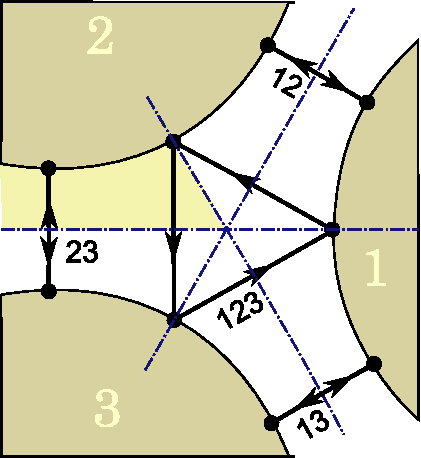
\includegraphics[width=0.25\textwidth]{3diskSymm-0}%
~~(b)~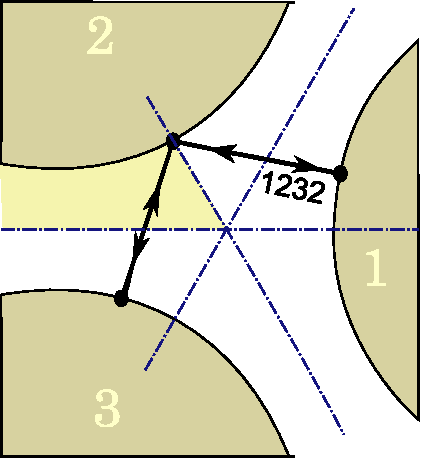
\includegraphics[width=0.25\textwidth]{3diskSymm-01}%
~~(c)~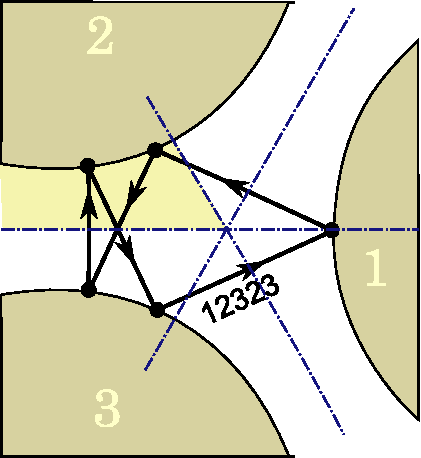
\includegraphics[width=0.25\textwidth]{3diskSymm-00111}
\vskip 2ex %\\
(d)~~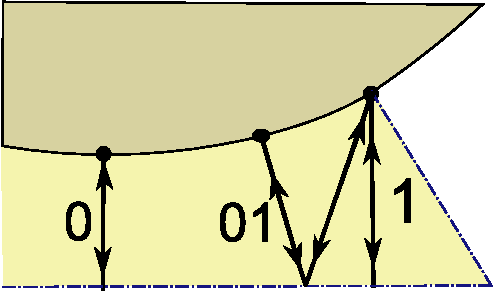
\includegraphics[width=0.25\textwidth]{3diskFundD}
  \end{minipage}
  \caption{\label{fig:3diskSymm}
% Following overhead on ChaosBook.org/overheads:
% \\
The 3-disk pinball {\orbit}s:
(a)
\cycle{12}, \cycle{13}, \cycle{23}, \cycle{123};
the clockwise \cycle{132} not drawn.
(b)
{\Orbit} \cycle{1232}; the symmetry related
\cycle{1213} and \cycle{1323} not drawn.
(c)
{\Orbit} \cycle{12323}; {\orbit}s \cycle{12123}, \cycle{12132}, \cycle{12313},
\cycle{13131} and \cycle{13232} not drawn.
(d) The fundamental domain, \ie, the light-shaded 1/6th wedge in
(a), consisting of a section of a disk, two segments of
symmetry axes acting as straight mirror walls, and the escape
gap to the left. The above 14 full-space {\orbit}s restricted to
the fundamental domain and recoded in binary reduce to the two
fixed points \cycle{0}, \cycle{1}, period-2 {\orbit} \cycle{10}, and
period-5 {\orbit} \cycle{00111} (not drawn).
% Radius~:~center separation ratio a:R~=~1:2.5.
}
\end{figure}
%%%%%%%%%%%%%%%%%%%%%%%%%%%%%%%%%%%%%%%%%%%%%%%%%%%

%%%%%%%%%%%%%%%%%%%%%%%%%%%%%%%%%%%%%%%%%%%%%%%%%%%%%%%%%%%%%%%%%%
\example{Subgroups, cosets of \Dn{3}.}{ \label{exam:C3cosets}
% examFiniteGr.tex called by \Chapter{finiteGr}{}{Flips, slides and turns}
\index{three-disk@3-disk!symmetry}\index{symmetry!3-disk}          \toCB
~~~(Continued from \refexam{exam:C3vInv})\\
The 3-disks symmetry group, the \Dn{3} dihedral group \refeq{groupD3}
has six subgroups
\beq
\{e\},\quad
\{e, \Refl\},\;
\{e, \Refl_{1}\},\;
\{e, \Refl_{2}\},\quad
\{e, \shift, \shift_2\},\quad
\Dn{3}
\,.
\ee{D3subgr}
The left cosets of subgroup $\Dn{1} = \{e, \Refl\}$ are
$\{\shift,\Refl_{1}\}$,
$\{\shift_2,\Refl_{2}\}$.
The coset of subgroup $\Cn{3} = \{e, \shift, \shift_2\}$ is
$\{\Refl,\Refl_{1},\Refl_{2}\}$. The significance of the
coset is that if a solution has a symmetry $H$, for example the symmetry
of a 3-cycle $\overline{123}$ is $\Cn{3}$, then all elements in a coset
act on it the same way, for example
$\{\Refl,\Refl_{1},\Refl_{2}\} \overline{123} = \overline{132}$.

The nontrivial subgroups of $\Dn{3}$ are $\Dn{1} = \{ e, \sigma \}$, consisting
of the identity and any one of the reflections, of order 2, and $\Cn{3} =
\{ e, \shift, \shift_2 \}$, of order $3$, so possible cycle
multiplicities are $|\Group|/|\Group_{p}| = 1$, $2$, $3$ or $6$. Only the
fixed point at the origin has full symmetry $\stab{p}=\Group$. Such
\eqva\ exist for smooth potentials, but not for the 3-disk billiard.
Examples of other multiplicities are given in \reffig{fig:3diskSymm} and
\reffig{dscr:fg3-exam}.
~~(continued in \refexam{exam:3diskClass})
                                        \jumpBack{exam:C3cosets}
    } %end \example{$D_3$ invariance - 3-disk game of pinball
%%%%%%%%%%%%%%%%%%%%%%%%%%%%%%%%%%%%%%%%%%%%%%%%%%%%%%%%%%%%%%%%%%

%% Classes of $\Dn{3}$.  % RETURN to ChaosBook
    % siminos/spatiotemp/Examples/exam3diskClass.tex
% $Author: predrag $ $Date: 2021-07-23 16:24:01 -0400 (Fri, 23 Jul 2021) $

%%%%%%%%%%%%%%%%%%%%%%%%%%%%%%%%%%%%%%%%%%%%%%%%%%%%%%%%%%%%%%%%%%
\example{Classes of $\Dn{3}$.}{ \label{exam:3diskClass}
% examFiniteGr.tex called by \Chapter{finiteGr}{}{Flips, slides and turns}
\index{three-disk@3-disk!symmetry}                            \toCB
\index{symmetry!3-disk}
(Continued from \refexam{exam:C3cosets})\\
The three classes of the 3-disk symmetry group
$\Dn{3} =\{ e, \shift, \shift_2,\Refl,\Refl_{1},\Refl_{2}\}$,
are the identity, any one of the reflections, and the two rotations,
 \beq
 \{ e \}\,,\quad
    \left\{\barr{c}
   \Refl     \\
   \Refl_{1} \\
   \Refl_{2}
    \earr\right\}
     \,,\quad
   \left\{\barr{c}
    \shift   \\
    \shift_2
    \earr\right\}
\,.
 \label{3diskClasses}
 \eeq
In other words, the group actions either flip or rotate.
~~(continued in \refexam{exam:C-3v-symm})
                                        \jumpBack{exam:3diskClass}
    } %end \example{3diskClass}
%%%%%%%%%%%%%%%%%%%%%%%%%%%%%%%%%%%%%%%%%%%%%%%%%%%%%%%%%%%%%%%%%%

%% Cyclic groups.   % RETURN to ChaosBook
    % siminos/spatiotemp/Examples/examCn.tex
% $Author: predrag $ $Date: 2021-07-23 16:15:21 -0400 (Fri, 23 Jul 2021) $

%%%%%%%%%%%%%%%%%%%%%%%%%%%%%%%%%%%%%%%%%%%%%%%%%%%%%%%%%%%%%%%%%%%%%%%
\example{Cyclic groups.}{  \label{exam:Cn}
% examFiniteGr.tex called by \Chapter{finiteGr}{}{Flips, slides and turns}
% started as M Field  Example 1.2.9., replaces \label{MField1-2-9}
\index{cyclic!group}                                               \toCB
\index{group!cyclic}
 The cyclic group
% Field calls it $Z_n$
$\Cn{n} \subset \SOn{2}$ (sometimes called \Zn{n}) of order $n$ is generated by one element
a shift \shift, the $1/n$ circle rotation by $2\pi/n$.
                                        \jumpBack{exam:Cn}
    } %end \example{}{  \label{exam:Cn}
%%%%%%%%%%%%%%%%%%%%%%%%%%%%%%%%%%%%%%%%%%%%%%%%%%%%%%%%%%%%%%%%%%%%%%%

%% XXX.
    % siminos/spatiotemp/Examples/examCnChars.tex
% $Author: predrag $ $Date: 2021-07-24 23:53:43 -0400 (Sat, 24 Jul 2021) $

%%%%%%%%%%%%%%%%%%%%%%%%%%%%%%%%%%%%%%%%%%%%%%%%%%%%%%%%%%%%%%%%%%%%%%
\example{Character table of cyclic group \Cn{n}.}{\label{exam:CnChars}
%% 2021-07-23 from Xiong's siminos/xiong/thesis/chapters/symGroup.tex
                                                                     \toCB
  The symmetry under a discrete rotation by angle $2\pi/n$ gives birth to a
  cyclic group $\Cn{n}=\{e,\shift,\shift^2,\cdots,\shift^{n-1}\}$.
  Since $\Cn{n}$ is Abelian, each element forms a separate class, and thus
  $\Cn{n}$ has $n$ one\dmn\ irreducible representations. The
  characters multiply as group elements:
  \(\chi_\alpha (\shift^i)\chi_\alpha
  (\shift^j)=\chi_{\alpha} (\shift^{i+j})
  \, \mod n
  \,.
  \)
  Therefore, we get \reftab{tab:CnChars}.
                                        \jumpBack{exam:CnChars}
\authorXD{}
}% end \example{exam:DnChars}
%%%%%%%%%%%%%%%%%%%%%%%%%%%%%%%%%%%%%%%%%%%%%%%%%%%%%%%%%%%%%%%%%%%%%%

%% Dihedral groups.  % RETURN to ChaosBook
    % siminos/spatiotemp/Examples/examDn.tex
% $Author: predrag $ $Date: 2021-07-23 16:15:21 -0400 (Fri, 23 Jul 2021) $

%%%%%%%%%%%%%%%%%%%%%%%%%%%%%%%%%%%%%%%%%%%%%%%%%%%%%%%%%%%%%%%%%%%%%%%
\example{Dihedral groups.}{  \label{exam:Dn}
% examFiniteGr.tex called by \Chapter{finiteGr}{}{Flips, slides and turns}
% started as M Field  Example 1.2.9., replaces \label{MField1-2-9}
\index{dihedral group}
\index{group!dihedral}                                    \toCB
The dihedral group
$\Dn{n} \subset \On{2}$, $n =1,2,3,\cdots$
(sometimes called \Cnv{n}),
can be generated by two elements one at least of which must
orientation reversing.
For example, take $\Refl$ corresponding to reflection across the
$x$-axis. $\Refl^2 = e$; such operation is called an
{\em involution}.
\index{involution}
$\shift{}$ to rotation through $2\pi/n$,
then $\Dn{n} = \langle \Refl,\shift \rangle$, and the defining relations are
$\Refl^2 = \shift^{n} = e$, $(\shift\Refl )^2 = e $.
                                        \jumpBack{exam:Dn}
    } %end \example{}{  \label{Dn}
%%%%%%%%%%%%%%%%%%%%%%%%%%%%%%%%%%%%%%%%%%%%%%%%%%%%%%%%%%%%%%%%%%%%%%%

%% \Dn{4} reflection symmetric, antisymmetric subspaces.
    % siminos/spatiotemp/Examples/examReflect4.tex
% $Author: predrag $ $Date: 2021-08-10 11:56:19 -0400 (Tue, 10 Aug 2021) $

%%%%%%%%%%%%%%%%%%%%%%%%%%%%%%%%%%%%%%%%%%%%%%%%%%%%%%%%%%%%%%%%%%
\example{\Dn{4} reflection symmetric, antisymmetric
         permutation representation subspaces.}
{ \label{exam:Reflect4}
The characteristic equation $\Refl^2=1$,
with eigenvalues $\{+1,-1\}$ , enables us to start the symmetry
reduction of the $\cl{}$\dmn\ permutation representation of $\Dn{\cl{}}$
by splitting it into the reflection symmetric or antisymmetric subspaces
by means of projection operators.

When the period  $\cl{}$ of the {\lattstate}s is even, there are two
classes of reflections.
For example, when the period of the {\lattstate}s is 4, reflection
operators $\Refl$ and $\Refl_1=\Refl\shift$ (see \refexam{exam:DinftyMultTab})
belong to distinct dihedral group
$\Dn{4}$ classes:
\beq
\Refl=
\left[
\begin{array}{cccc}
 0 & 0 & 0 & 1 \\
 0 & 0 & 1 & 0 \\
 0 & 1 & 0 & 0 \\
 1 & 0 & 0 & 0 \\
\end{array}
\right]
\,,\quad
\Refl_1=
\left[
\begin{array}{cccc}
 0 & 0 & 1 & 0 \\
 0 & 1 & 0 & 0 \\
 1 & 0 & 0 & 0 \\
 0 & 0 & 0 & 1\\
\end{array}
\right] \, ,
\ee{PCreflect4}
where $\shift$ is the shift matrix.
Either one splits the
$\cl{}$\dmn\ permutation representation of $\Dn{\cl{}}$
into the reflection symmetric and antisymmetric subspaces.
For $\Refl$ the two  projection operators are
\bea
\PP_{0+} &=& \frac{\Refl - (-1) \unit}{1-(-1)} =
\frac{1}{2}
\left[
\begin{array}{cccc}
 1 & 0 & 0 & 1 \\
 0 & 1 & 1 & 0 \\
 0 & 1 & 1 & 0 \\
 1 & 0 & 0 & 1
\end{array}
\right]
                   \continue
\PP_{0-} &=& \frac{~\Refl - \unit}{-1-1} =
\frac{1}{2}
\left[
\begin{array}{cccc}
 1 & 0 & 0 & -1 \\
 0 & 1 & -1 & 0 \\
 0 & -1 & 1 & 0 \\
 -1 & 0 & 0 & 1 \\
\end{array}
\right]
\,,
\label{Reflect4Refl}
\eea
and
for $\Refl_1$ they are
\bea
\PP_{1+} &=& \frac{\unit-(-1)\Refl_1}{1+1} =
\frac{1}{2}
\left[
\begin{array}{cccc}
 1 & 0 & 1 & 0 \\
 0 & 2 & 0 & 1 \\
 1 & 0 & 1 & 0 \\
 0 & 0 & 0 & 2 \\
\end{array}
\right]
                   \continue
\PP_{1-} &=& \frac{\unit+(-1)\Refl_1}{1+1} =
\frac{1}{2}
\left[
\begin{array}{cccc}
 1 & 0 &-1 & 0 \\
 0 & 0 & 0 & 0 \\
-1 & 0 & 1 & 0 \\
 0 & 0 & 0 & 0 \\
\end{array}
\right]
\,.
\label{Reflect4reflShift}
\eea
Either splits the $\cl{}$\dmn\ permutation representation, but in a
different way. The dimensions $d_\alpha=\Tr\PP_\alpha$ of the pairs of
subspaces are
$d_{\Refl+}=2$,
$d_{\Refl-}=2$,
and
$d_{\Refl_1+}=3$,
$d_{\Refl_1-}=1$.
They are reducible further by each other, and
by the translation operator characteristic equation $\shift^4=1$.
Of course, there is no reason to single out reflection operators $\Refl$
and $\Refl_1$. For a systematic, all commuting operator approach, see
\refexam{exam:D6mult} for the Burnside, class operator full reduction.
                                        \jumpBack{exam:Reflect4}
} % end {exam:Reflect4}
%%%%%%%%%%%%%%%%%%%%%%%%%%%%%%%%%%%%%%%%%%%%%%%%%%%%%%%%%%%%%%%%%%

%% \Dn{6} reflection symmetric, antisymmetric subspaces.
    % siminos/spatiotemp/Examples/examReflect6.tex
% $Author: predrag $ $Date: 2021-08-10 11:56:19 -0400 (Tue, 10 Aug 2021) $

%%%%%%%%%%%%%%%%%%%%%%%%%%%%%%%%%%%%%%%%%%%%%%%%%%%%%%%%%%%%%%%%%%
\example{\Dn{6} reflection symmetric, antisymmetric
         permutation representation subspaces.}
{ \label{exam:Reflect6}
%  from 2021-05-11 Han, siminos/spatiotemp/chapter/blogHL.tex
The characteristic equation $\Refl^2=1$,
with eigenvalues $\{+1,-1\}$ , enables us to start the symmetry
reduction of the $\cl{}$\dmn\ permutation representation of $\Dn{\cl{}}$
by splitting it into the reflection symmetric or antisymmetric subspaces
by means of projection operators.

When the period  $\cl{}$ of the {\lattstate}s is even, there are two
classes of reflections.
For example, when the period of the {\lattstate}s is 6, reflection
operators $\Refl$ and $\shift\Refl$ belong to distinct dihedral group
$\Dn{6}$ classes:
\beq
\Refl=
\left[
\begin{array}{cccccc}
 0 & 0 & 0 & 0 & 0 & 1 \\
 0 & 0 & 0 & 0 & 1 & 0 \\
 0 & 0 & 0 & 1 & 0 & 0 \\
 0 & 0 & 1 & 0 & 0 & 0 \\
 0 & 1 & 0 & 0 & 0 & 0 \\
 1 & 0 & 0 & 0 & 0 & 0 \\
\end{array}
\right] \, ,
\ee{HLreflect6}
and
    \PC{2021-07-25}{
I would prefer $\Refl_1=\Refl\shift$, to be consistent with the wiki
convention of \refexam{exam:DinftyMultTab}.
    }
\beq
\shift\Refl=
\left[
\begin{array}{cccccc}
 1 & 0 & 0 & 0 & 0 & 0 \\
 0 & 0 & 0 & 0 & 0 & 1 \\
 0 & 0 & 0 & 0 & 1 & 0 \\
 0 & 0 & 0 & 1 & 0 & 0 \\
 0 & 0 & 1 & 0 & 0 & 0 \\
 0 & 1 & 0 & 0 & 0 & 0 \\
\end{array}
\right] \, ,
\ee{HLreflect6other}
where $\shift$ is the shift matrix.
Either one splits the
$\cl{}$\dmn\ permutation representation of $\Dn{\cl{}}$
into the reflection symmetric and antisymmetric subspaces.
For $\Refl$ the two  projection operators are
\bea
\PP_{0+} &=& \frac{\Refl - (-1) \unit}{1-(-1)} =
\frac{1}{2}
\left[
\begin{array}{cccccc}
 1 & 0 & 0 & 0 & 0 & 1 \\
 0 & 1 & 0 & 0 & 1 & 0 \\
 0 & 0 & 1 & 1 & 0 & 0 \\
 0 & 0 & 1 & 1 & 0 & 0 \\
 0 & 1 & 0 & 0 & 1 & 0 \\
 1 & 0 & 0 & 0 & 0 & 1 \\
\end{array}
\right]
                   \continue
\PP_{1-} &=& \frac{\shift \Refl - \unit}{-1-1} =
\frac{1}{2}
\left[
\begin{array}{cccccc}
 0 & 0 & 0 & 0 & 0 & 0 \\
 0 & 1 & 0 & 0 & 0 & -1 \\
 0 & 0 & 1 & 0 & -1 & 0 \\
 0 & 0 & 0 & 0 & 0 & 0 \\
 0 & 0 & -1 & 0 & 1 & 0 \\
 0 & -1 & 0 & 0 & 0 & 1 \\
\end{array}
\right]
\,,
\label{Reflect6Refl}
\eea
and
for $\shift\Refl$ they are
\bea
\PP_{0-} &=& \frac{~\Refl - \unit}{-1-1} =
\frac{1}{2}
\left[
\begin{array}{cccccc}
 1 & 0 & 0 & 0 & 0 & -1 \\
 0 & 1 & 0 & 0 & -1 & 0 \\
 0 & 0 & 1 & -1 & 0 & 0 \\
 0 & 0 & -1 & 1 & 0 & 0 \\
 0 & -1 & 0 & 0 & 1 & 0 \\
 -1 & 0 & 0 & 0 & 0 & 1 \\
\end{array}
\right]
                   \continue
\PP_{1+} &=& \frac{\shift \Refl - (-1) \unit}{1-(-1)} =
\frac{1}{2}
\left[
\begin{array}{cccccc}
 2 & 0 & 0 & 0 & 0 & 0 \\
 0 & 1 & 0 & 0 & 0 & 1 \\
 0 & 0 & 1 & 0 & 1 & 0 \\
 0 & 0 & 0 & 2 & 0 & 0 \\
 0 & 0 & 1 & 0 & 1 & 0 \\
 0 & 1 & 0 & 0 & 0 & 1 \\
\end{array}
\right]
\,.
\label{Reflect6shiftRefl}
\eea
Either splits the $\cl{}$\dmn\ permutation representation, but in a
different way. The dimensions $d_\alpha=\Tr\PP_\alpha$ of the pairs of
subspaces are
$d_{0+}=3$,
$d_{0-}=3$,
and
$d_{1+}=4$,
$d_{1-}=2$.
They are reducible further by each other, and
by the translation operator characteristic equation $\shift^6=1$.
Of course, there is no reason to single out reflection operators $\Refl$
and $\shift\Refl$. For a systematic, all commuting operator approach, see
\refexam{exam:D6mult} for the Burnside, class operator full reduction.
                                        \jumpBack{exam:Reflect6}
\authorHL{2021-05-11}
} % end {exam:Reflect6}
%%%%%%%%%%%%%%%%%%%%%%%%%%%%%%%%%%%%%%%%%%%%%%%%%%%%%%%%%%%%%%%%%%

%% XXX.
    % siminos/spatiotemp/Examples/examD3permRep.tex
% $Author: predrag $ $Date: 2021-08-10 11:56:19 -0400 (Tue, 10 Aug 2021) $

%%%%%%%%%%%%%%%%%%%%%%%%%%%%%%%%%%%%%%%%%%%%%%%%%%%%%%%%%%%%%%%%%%%%%
\example{\Dn{3} multiplication tables and the permutation rep.}{
\label{exam:D3permRep}
For period-3 {\lattstate}s, the
class operators are the identity $\id$ and
\beq
{\cal R}=
\left[
\begin{array}{ccc}
 0 & 1 & 1 \\
 1 & 0 & 1 \\
 1 & 1 & 0
\end{array}
\right] \,,\quad
{\cal S}=
\left[
\begin{array}{ccc}
 1 & 1 & 1 \\
 1 & 1 & 1 \\
 1 & 1 & 1
\end{array}
\right] = \id+{\cal R}
\,,
\ee{D3RS}
so either ${\cal R}$ or ${\cal S}$ can be eliminated from the class
multiplication \reftab{tab:D3multTab}. In the spirit of the presentation of a
dihedral group in terms of two flips, let's eliminate ${\cal R}={\cal S}-\id$:
\beq
\begin{tabular}{c|cc|}
\Dn{3}      &\id        &${\cal S}$\\\hline
\id         &\id        &${\cal S}$\\
${\cal S}$  &${\cal S}$ &$3\,{\cal S}$\\\hline
\end{tabular}
\ee{tab:D3multClasPerm}
From this \Dn{3} class operator multiplication table follows the
Hamilton-Cayley equation
for its 3\dmn\
permutation rep, with two eigenvalues,
\beq
{\cal S}({\cal S} - 3\id) = 0
\,,
\label{D3Ham-CayPerm}
\eeq
with projection operators
\beq
\begin{tabular}{l|rl|r}
$\lambda$&               & projection op.        &$d$ \\\hline
3        &$\PP_{3} =$    &${\cal S}/3$           &1 \\
0        &$\PP_{0} =$    &$(3\id - {\cal S})/3$  &2 \\\hline
\end{tabular}
\ee{tab:Ham-CayD3proj}
Note that the zero-eigenvalue $\PP_{0}$ is the Laplacian operator.

Take {\jacobianOrb} of form common to both the \templatt\
\refeq{jMorbInfin} and the \henlatt\ \refeq{Henlatt-orbitJac}, and
use the spectral resolution $\id=\PP_{0}+\PP_{3}$:
\beq
d=3 \qquad\qquad
\jMorb=
\left[
\begin{array}{ccc}
-\jMorb_{00} & 1           & 1 \\
          1  &-\jMorb_{11} & 1 \\
          1  & 1           & -\jMorb_{22}
\end{array}
\right] = \PP_{0} - (\jMorb-\id)
\,,
\ee{D3orbJac}

Study also
\HREF{https://en.wikipedia.org/wiki/Permutation_representation\#Character_of_the_permutation_representation}
{wiki: {\em Character of the permutation representation}}.

Dixon, J. D. and Mortimer, {\em Permutation Groups}, Springer
%ISBN 9781461207313.

        \jumpBack{exam:D3permRep}
    } % end {exam:D3permRep}
%%%%%%%%%%%%%%%%%%%%%%%%%%%%%%%%%%%%%%%%%%%%%%%%%%%%%%%%%%%%%%%%%%%%%

%% XXX.
    % siminos/spatiotemp/Examples/examD6mult.tex
% $Author: predrag $ $Date: 2021-08-25 23:18:52 -0400 (Wed, 25 Aug 2021) $

%%%%%%%%%%%%%%%%%%%%%%%%%%%%%%%%%%%%%%%%%%%%%%%%%%%%%%%%%%%%%%%%%%%%%%
% Predrag                                                   2021-06-14
\begin{table}
\caption[]{
The \Dn{6} Cayley  table (group multiplication \refeq{eq:DinftyMultTab}
table), and the class operator multiplication table.
The class operator multiplication table is symmetric under transposition,
so it suffices to fill up the upper half-triangular region. The 6 classes
correspond to 4 1\dmn\ irreps, and the 2 1\dmn\ irreps.
    }
\begin{center}
\begin{tabular}{c||c|c|cc|cc|ccc|ccc|}
\Dn{6}&$1  $ &$r^3$ &$r  $ &$r^5$ &$r^2$ &$r^4$ &$s  $ &$s_2$ &$s_4$ &$s_1$ &$s_3$ &$s_5$\\\hline\hline
$1  $ &$1  $ &$r^3$ &$r  $ &$r^5$ &$r^2$ &$r^4$ &$s  $ &$s_2$ &$s_4$ &$s_1$ &$s_3$ &$s_5$\\ \hline
$r^3$ &$r^3$ &$1  $ &$r^4$ &$r^2$ &$r^5$ &$r  $ &$s_3$ &$s_5$ &$s_1$ &$s  $ &$s_1$ &$s_2$\\ \hline
$r  $ &$r  $ &$r^4$ &$r^2$ &$1  $ &$r^3$ &$r^5$ &$s_1$ &$s_3$ &$s_5$ &$s_2$ &$s_4$ &$s  $\\
$r^5$ &$r^5$ &$r^2$ &$1  $ &$r^4$ &$r  $ &$r^3$ &$s_5$ &$s_1$ &$s_3$ &$s  $ &$s_2$ &$s_4$\\ \hline
$r^2$ &$r^2$ &$r^5$ &$r^3$ &$r  $ &$r^4$ &$1  $ &$s_2$ &$s_4$ &$s  $ &$s_3$ &$s_5$ & $s_1$\\
$r^4$ &$r^4$ &$r  $ &$r^5$ &$r^3$ &$1  $ &$r^2$ &$s_4$ &$s  $ &$s_2$ &$s_5$ &$s_1$ &$s_3$\\ \hline
$s  $ &$s  $ &$s_3$ &$s_1$ &$s_5$ &$s_2$ &$s_4$ &$1  $ &$r^4$ &$r^2$ &$r^5$ &$r^3$ &$r $\\
$s_2$ &$s_2$ &$s_5$ &$s_3$ &$s_1$ &$s_4$ &$s  $ &$r^2$ &$1  $ &$r^4$ &$r  $ &$r^5$ &$r^3$\\
$s_4$ &$s_4$ &$s_2$ &$s_5$ &$s_3$ &$s  $ &$s_2$ &$r^4$ &$r^2$ &$1  $ &$r^3$ &$r  $ &$r^5$\\ \hline
$s_1$ &$s_1$ &$s_4$ &$s_2$ &$s  $ &$s_3$ &$s_5$ &$r  $ &$r^5$ &$r^3$ &$1  $ &$r^4$ &$r^2$\\
$s_3$ &$s_3$ &$s  $ &$s_4$ &$s_2$ &$s_5$ &$s_1$ &$r^3$ &$r  $ &$r^5$ &$r^2$ &$1  $ &$r^4$\\
$s_5$ &$s_5$ &$s_3$ &$s  $ &$s_4$ &$s_1$ &$s_3$ &$r^5$ &$r^3$ &$r  $ &$r^4$ &$r^2$ &$1  $\\
\hline%$[2ex]
\end{tabular}
\bigskip

\begin{tabular}{c|c c c c c c|}
\Dn{6}&\id&\ensuremath{{\cal R}_{3}}&\ensuremath{{\cal R}_{1}}&\ensuremath{{\cal R}_{2}}&\ensuremath{{\cal S}_{0}}&\ensuremath{{\cal S}_{1}}\\\hline
\id   &\id      &\ensuremath{{\cal R}_{3}}  &\ensuremath{{\cal R}_{1}}&\ensuremath{{\cal R}_{2}}      &\ensuremath{{\cal S}_{0}}&\ensuremath{{\cal S}_{1}}\\
\ensuremath{{\cal R}_{3}}&.&\id&\ensuremath{{\cal R}_{2}}  &\ensuremath{{\cal R}_{1}}&\ensuremath{{\cal S}_{1}}&\ensuremath{{\cal S}_{0}}\\
\ensuremath{{\cal R}_{1}}&.&.&2\id+\ensuremath{{\cal R}_{2}} &2\ensuremath{{\cal R}_{3}}+\ensuremath{{\cal R}_{1}} &2\ensuremath{{\cal S}_{1}}&2\ensuremath{{\cal S}_{0}}\\
\ensuremath{{\cal R}_{2}}&.&.&.&2\id+\ensuremath{{\cal R}_{2}} &2\ensuremath{{\cal S}_{0}}&2\ensuremath{{\cal S}_{1}}\\
\ensuremath{{\cal S}_{0}}&.&.&.&.&3(\id+\ensuremath{{\cal R}_{2}})&3(\ensuremath{{\cal R}_{3}}+\ensuremath{{\cal R}_{1}})\\
\ensuremath{{\cal S}_{1}}&.&.&.&.&.&3(\id+\ensuremath{{\cal R}_{2}})\\\hline
\end{tabular}
\end{center}
  \label{tab:D6multTab}
\end{table}
%%%%%%%%%%%%%%%%%%%%%%%%%%%%%%%%%%%%%%%%%%%%%%%%%%%%%%%%%%%%%%%%%%%%%%

%%%%%%%%%%%%%%%%%%%%%%%%%%%%%%%%%%%%%%%%%%%%%%%%%%%%%%%%%%%%%%%%%%%%%
\example{\Dn{6} multiplication tables.}{\label{exam:D6mult}
From the \Dn{6} class operator multiplication table follow the
Hamilton-Cayley equations (for any matrix representation; in our application
\refeq{PCreflect} that is the 6\dmn\ matrix
representation of permutations), with 16 eigenvalues as listed,
    \PC{2021-06-16}{${\cal R}_{2}$ is a guess, I have not derived it.}
\bea
({\cal R}_{3} - \id)({\cal R}_{3} + \id) &=& 0
    \continue
({\cal R}_{1} - \id)({\cal R}_{1} + \id)
({\cal R}_{1} - 2\id)({\cal R}_{1} + 2\id) &=& 0
    \continue
({\cal R}_{2} - \id)({\cal R}_{2} + \id)
({\cal R}_{2} - 2\id)({\cal R}_{2} + 2\id) &=& 0
    \continue
{\cal S}_{0}
({\cal S}_{0} - 3\id)({\cal S}_{0} + 3\id) &=& 0
    \continue
{\cal S}_{1}
({\cal S}_{1} - 3\id)({\cal S}_{1} + 3\id) &=& 0
\,,
\label{Ham-CayD6}
\eea
so there is lots of redundancy - there are only 6 irreps.
\bea
{\cal R}_{3}:\; \lambda=1 &\rightarrow& \qquad
\PP_{1} = (\id+{\cal R}_{3})/2
     \continue
{\cal R}_{3}:\; \lambda=-1 &\rightarrow& \qquad
\PP_{-1} = (\id-{\cal R}_{3})/2
     \continue
{\cal S}_{0}:\; \lambda=0 &\rightarrow& \qquad
\PP_{0,0}
%    = ({\cal S}_{0} - 3\id)({\cal S}_{0} + 3\id)/9
%    = (9\id -{\cal S}_{0}^2)/9
    =  (2\id - {\cal R}_{2})/3
    \continue
{\cal S}_{0}:\; \lambda=3 &\rightarrow& \qquad
\PP_{0,3}
    %= {\cal S}_{0}({\cal S}_{0} + 3\id)/3\cdot6
    = (\id+{\cal R}_{2}+{\cal S}_{0})/6
     \continue
{\cal S}_{0}:\; \lambda=-3 &\rightarrow& \qquad
\PP_{0,-3}
%    = {\cal S}_{0}({\cal S}_{0} - 3\id)/3\cdot6
    = (\id+{\cal R}_{2} - {\cal S}_{0})/6
     \continue
{\cal S}_{1}:\; \lambda=0 &\rightarrow& \qquad
\PP_{1,0}
%    = ({\cal S}_{0} - 3\id)({\cal S}_{0} + 3\id)/9
%   = (9\id -{\cal S}_{1}^2)/9
%   =  (2\id - {\cal R}_{2})/3
    = \PP_{0:\;0}
     \continue
{\cal S}_{1}:\; \lambda=3 &\rightarrow& \qquad
\PP_{1,3}
%    = {\cal S}_{0}({\cal S}_{0} - 3\id)/3\cdot6
    = (\id+{\cal R}_{2} + {\cal S}_{1})/6
   \continue
{\cal S}_{1}:\; \lambda=-3 &\rightarrow& \qquad
\PP_{1,-3}
    = (\id+\ensuremath{{\cal R}_{2}} - {\cal S}_{1})/3
\,.
\label{Ham-CayD6S0S1PP}
\eea
Split $\PP_{0,-3}$ using $\PP_{1}$:
\bea
\PP_{1}\PP_{0,-3}
%    &=& (\id+{\cal R}_{3})(\id+{\cal R}_{2} - {\cal S}_{0})/2.6
%     \continue
    &=& (\id+{\cal R}_{3}+{\cal R}_{1}+{\cal R}_{2} - {\cal S}_{0} - {\cal S}_{1})/12
\,.
\label{Ham-CayD6PPpm1}
\eea


${\cal S}_{j}$ equations are the same form as for $\Dn{3}$ 1\dmn\ irrep, so
the number of such equations presumably equals the number of 1\dmn\ irrep,
and the same for ${\cal R}_{j}$, $j\neq n/2$ equations.

${\cal S}_{j}$ equations presumably contain symmetric/antisymmetric 
solutions, in the spirit of \refeq{HLreflect6} and \refeq{HLreflect6other}.

For even dimensions
${\cal R}_{n/2}$ presumably leads to 4 1\dmn\ irreps, of which I assume the
two antisymmetric ones do not contribute to the$n$\dmn\ matrix representation
of permutations, while all 1\dmn\ irrep do.

That is probably easier to count using the character formulas.

       \jumpBack{exam:D6mult}
    } % end {exam:exam:D6mult}
%%%%%%%%%%%%%%%%%%%%%%%%%%%%%%%%%%%%%%%%%%%%%%%%%%%%%%%%%%%%%%%%%%%%%

%% XXX.
    % siminos/spatiotemp/Examples/examD6permRep.tex
% $Author: predrag $ $Date: 2021-08-10 11:56:19 -0400 (Tue, 10 Aug 2021) $

%%%%%%%%%%%%%%%%%%%%%%%%%%%%%%%%%%%%%%%%%%%%%%%%%%%%%%%%%%%%%%%%%%%%%
\example{\Dn{6} permutation rep.}{\label{exam:D6permRep}
For period-6 {\lattstate}s, the
class operators are the identity, and:
\beq
{\cal R}_{3}=
\left[
\begin{array}{cccccc}
 0 & 0 & 0 & 1 & 0 & 0 \\
 0 & 0 & 0 & 0 & 1 & 0 \\
 0 & 0 & 0 & 0 & 0 & 1 \\
 1 & 0 & 0 & 0 & 0 & 0 \\
 0 & 1 & 0 & 0 & 0 & 0 \\
 0 & 0 & 1 & 0 & 0 & 0 \\
\end{array}
\right] \,,\quad
\ee{D6R3}

\beq
{\cal R}_{1}=
\left[
\begin{array}{ccc|ccc}
 0 & 1 & 0 & 0 & 0 & 1 \\
 1 & 0 & 1 & 0 & 0 & 0 \\
 0 & 1 & 0 & 1 & 0 & 0 \\\hline
 0 & 0 & 1 & 0 & 1 & 0 \\
 0 & 0 & 0 & 1 & 0 & 1 \\
 1 & 0 & 0 & 0 & 1 & 0 \\
\end{array}
\right] \,,\quad
{\cal R}_{2}=
\left[
\begin{array}{ccc|ccc}
 0 & 0 & 1 & 0 & 1 & 0 \\
 0 & 0 & 0 & 1 & 0 & 1 \\
 1 & 0 & 0 & 0 & 1 & 0 \\\hline
 0 & 1 & 0 & 0 & 0 & 1 \\
 1 & 0 & 1 & 0 & 0 & 0 \\
 0 & 1 & 0 & 1 & 0 & 0
\end{array}
\right] \,.
\ee{D6R1R2}

\beq
{\cal S}_{0}=
\left[
\begin{array}{ccc|ccc}
 0 & 1 & 0 & 1 & 0 & 1 \\
 1 & 0 & 1 & 0 & 1 & 0 \\
 0 & 1 & 0 & 1 & 0 & 1 \\\hline
 1 & 0 & 1 & 0 & 1 & 0 \\
 0 & 1 & 0 & 1 & 0 & 1 \\
 1 & 0 & 1 & 0 & 1 & 0 \\
\end{array}
\right]
\,,\quad
{\cal S}_{1}=
\left[
\begin{array}{ccc|ccc}
 1 & 0 & 1 & 0 & 1 & 0 \\
 0 & 1 & 0 & 1 & 0 & 1 \\
 1 & 0 & 1 & 0 & 1 & 0 \\\hline
 0 & 1 & 0 & 1 & 0 & 1 \\
 1 & 0 & 1 & 0 & 1 & 0 \\
 0 & 1 & 0 & 1 & 0 & 1
\end{array}
\right] \,.
\ee{PCreflect6}
The reflection operators eigenvalues are $+1$ and $-1$,
corresponding to the reflection symmetric and antisymmetric subspaces.

To compute the dimensions of irreps obtained from
\refeq{Ham-CayD6}, we need the characters of the permutation representation
class operators:
\beq
\tr{\id}=6\,,\;
\tr{{\cal R}_{3}}=0\,,\;
\tr{{\cal R}_{1}}=0\,,\;
\tr{{\cal R}_{2}}=0\,,\;
\tr{{\cal S}_{0}}=0\,,\;
\tr{{\cal S}_{1}}=6
\,.
\ee{D6clasOpsTr}
(Predrag: I do not see why ${\cal S}_{1}$ is special...)
In particular, we have a vanishing dimension
$\lambda=-3$ representation, so
\bea
{\cal S}_{1}, \lambda=-3 &\rightarrow& \qquad
\PP_{1,-3}
    = (\id+\ensuremath{{\cal R}_{2}} - {\cal S}_{1})/2
    = 0
\,,
\label{Ham-CayD6zero}
\eea
Taking trace of \refeq{Ham-CayD6PPpm1} we find that also $\PP_{1}\PP_{0,-3}$
is 0\dmn, so, 6\dmn\ permutation representation is not faithful, and the
classes are not independent (you can check this by inspecting eqs.
\refeq{PCreflect6} to \refeq{D6R1R2}):
\bea
{\cal S}_{0} &=& {\cal R}_{3} + {\cal R}_{1}
    \continue
{\cal S}_{1} &=& \id + {\cal R}_{2}
\,,
\label{D6PermClassOps}
\eea
so forget the last two equations in \refeq{Ham-CayD6} for the $\cl{}$\dmn\
permutation representations of \Dn{\cl{}}. I think it is clear from
\refeq{Ham-CayD6PPpm1} that this means no
antisymmetric 1\dmn\ reps.

Lecturing about the "projector analysis" of \Dn{3} I was such a fool - I
forgot to follow \wwwgt{}, which explains very clearly that whenever there is
a matrix equation =0, that means a relationship between matrices, they are
not independent.

Now one can eliminate ${\cal S}_{j}$ from projection operators \refeq{Ham-CayD6S0S1PP}:
\bea
{\cal S}_{0}:\; \lambda=3 &\rightarrow& \qquad
\PP_{0,3}
    %= {\cal S}_{0}({\cal S}_{0} + 3\id)/3\cdot6
    = (\id+{\cal R}_{3}+{\cal R}_{1} + {\cal R}_{2})/6
    \continue{\cal S}_{1}:\; \lambda=3 &\rightarrow& \qquad
\PP_{1,3}
%    = {\cal S}_{0}({\cal S}_{0} - 3\id)/3\cdot6
    = (\id+{\cal R}_{2})/3
\,,
\label{am-CayD6S0S1PP1}
\eea
To summarize - this is rather inelegant, but the main result is that the flip
classes ${\cal S}_{0},{\cal S}_{1},{\cal S}_{2},\cdots$ do not contribute to
the reduction of the permutation representation; is can be done purely in
terms of the rotation classes
${\cal R}_{1},{\cal R}_{3},{\cal R}_{3},\cdots$. This strikes me as a big
deal, as this is isomorphic - I believe - to the cyclic group \Cn{\cl{}/2}
(for the even period $\cl{}$). I tentative submit \reftab{tab:D6multTabperm}
being sufficient to construct all irreducible projection operators. Of
course, \Cn{6} is the only normal subgroup of \Dn{6}, but we do not use that
- we use only 4 classes rather than the 6 of \Cn{6}. Looks pretty illegal:)

Can you check that you get 2 symmetric
1\dmn\ irreps, and the two 1\dmn\ ones?
        \jumpBack{exam:D6permRep}
} % end \example{exam:D6permRep}
%%%%%%%%%%%%%%%%%%%%%%%%%%%%%%%%%%%%%%%%%%%%%%%%%%%%%%%%%%%%%%%%%%%%%


%%%%%%%%%%%%%%%%%%%%%%%%%%%%%%%%%%%%%%%%%%%%%%%%%%%%%%%%%%%%%%%%%%%%%%
% Predrag                                                   2021-06-14
\begin{table}
\caption[]{
A tentative \Dn{6} class operator multiplication table restricted to the
permutations matrix representation, with flip classes eliminated using
\refeq{D6PermClassOps}.
    }
\begin{center}
\begin{tabular}{c|c c c c|}
\Dn{6}&\id&\ensuremath{{\cal R}_{3}}&\ensuremath{{\cal R}_{1}}&\ensuremath{{\cal R}_{2}}\\\hline
\id   &\id      &\ensuremath{{\cal R}_{3}}  &\ensuremath{{\cal R}_{1}}&\ensuremath{{\cal R}_{2}}\\
\ensuremath{{\cal R}_{3}}&.&\id&\ensuremath{{\cal R}_{2}}  &\ensuremath{{\cal R}_{1}}\\
\ensuremath{{\cal R}_{1}}&.&.&2\id+\ensuremath{{\cal R}_{2}} &2\ensuremath{{\cal R}_{3}}+\ensuremath{{\cal R}_{1}}\\
\ensuremath{{\cal R}_{2}}&.&.&.&2\id+\ensuremath{{\cal R}_{2}}\\\hline
\end{tabular}
\end{center}
  \label{tab:D6multTabperm}
\end{table}
%%%%%%%%%%%%%%%%%%%%%%%%%%%%%%%%%%%%%%%%%%%%%%%%%%%%%%%%%%%%%%%%%%%%%%

%% XXX.
    % siminos/spatiotemp/Examples/examDnOddChars.tex
% $Author: predrag $ $Date: 2021-07-25 19:52:46 -0400 (Sun, 25 Jul 2021) $

%%%%%%%%%%%%%%%%%%%%%%%%%%%%%%%%%%%%%%%%%%%%%%%%%%%%%%%%%%%%%%%%%%%%%%
\begin{table}[h]
  \caption[Character table of cyclic group \Cn{n}]{
    Character table of cyclic group \Cn{n}. Here $k,j=1,2,\cdots,n-1$.
  }
  \label{tab:CnChars}
  \begin{center}
    \begin{tabular}{c|cr}
      $\Cn{n}$       & $A$& $\Gamma_{j}$ \\
      \hline
      $  e  $        &   1  &   1  \\
      $\shift^{k} $     &   1  &   $\exp(\frac{i2\pi kj}{n})$   \\
    \end{tabular}
  \end{center}
\end{table}
%%%%%%%%%%%%%%%%%%%%%%%%%%%%%%%%%%%%%%%%%%%%%%%%%%%%%%%%%%%%%%%%%%%%%%%

%%%%%%%%%%%%%%%%%%%%%%%%%%%%%%%%%%%%%%%%%%%%%%%%%%%%%%%%%%%%%%%%%%%%%%
\example{Character table of dihedral group $\Dn{n}$, $n$ odd.}{ %$=C_{nv}$}{
  \label{exam:DnOddChars}                                           \toCB
%% 2021-07-23 from Xiong's siminos/xiong/thesis/chapters/symGroup.tex
  The  \Dn{n} group
  \[
    \Dn{n}=\{e,\shift,\shift^2,\cdots,\shift^{n-1},\Refl,\shift\Refl,\cdots,
    \shift^{n-1}\Refl\}
  \]
  has
  $n$ rotation elements and $n$ reflections.
  Group elements satisfies $\shift^i\cdot \shift^j\Refl=\shift^j\Refl\cdot \shift^{n-i}$,
  so $\shift^i$ and $\shift^{n-i}$ form a class. Also,
  $\shift^{n-i}\cdot \shift^{2i+j}\Refl=\shift^j\Refl\cdot \shift^{n-i}$ implies that
  $\shift^j\Refl$ and $\shift^{2i+j}\Refl$ are in the same class. Therefore,
  there are only three different types of classes:
  $\{e\}$, $\{\shift^k,\shift^{n-k}\}$ and
  $\{\Refl,\shift\Refl,\cdots, \shift^{n-1}\Refl\}$. The total number of
  classes is $(n+3)/2$. In this case, there are 2 one\dmn\
  irreducible representations (symmetric $A_1$ and antisymmetric $A_2$ )
  and $(n-1)/2$ two\dmn\ irreducible representations. In the $j$th
  two\dmn\ irreducible representation, class $\{e\}$ has form
  $\bigl(\begin{smallmatrix}
    1&0\\ 0&1
  \end{smallmatrix} \bigr)$,
  class $\{\shift^k,\shift^{n-k}\}$ has form
  $\bigl(\begin{smallmatrix}
    \exp(\frac{i2\pi kj}{n}) &0 \\ 0& \exp(-\frac{i2\pi kj}{n})
  \end{smallmatrix} \bigr)$,
  and class $\{\Refl,\shift\Refl,\cdots, \shift^{n-1}\Refl\}$ has form
  $\bigl(\begin{smallmatrix}
    0&1\\ 1&0
  \end{smallmatrix} \bigr)$.
  We get \reftab{tab:DnOdd}.
                                        \jumpBack{exam:DnOddChars}
\authorXD{}
}% end \example{exam:DnOddChars}
%%%%%%%%%%%%%%%%%%%%%%%%%%%%%%%%%%%%%%%%%%%%%%%%%%%%%%%%%%%%%%%%%%%%%%

%% XXX.
    % siminos/spatiotemp/Examples/examDnEvenChars.tex
% $Author: predrag $ $Date: 2021-10-13 18:02:53 -0400 (Wed, 13 Oct 2021) $

%%%%%%%%%%%%%%%%%%%%%%%%%%%%%%%%%%%%%%%%%%%%%%%%%%%%%%%%%%%%%%%%%%%%%%
\begin{table}[h]
  \caption[Character table of dihedral group $\Dn{n}$, $n$ odd.]{
    Character table of dihedral group $\Dn{n}$, $n$ odd.
  }
  \label{tab:DnOdd}
  \begin{center}
    \begin{tabular}{c|ccc}
      $\Dn{n}$ ($n$ odd)  & $A_1$& $A_2$& $E_{j}$ \\
      \hline
      $  e  $        &   1  &   1  &  2 \\
      $\shift^k,\shift^{n-k} $ &   1  &   1  &  $2\cos(\frac{2\pi kj}{n})$ \\
      $\Refl,\Refl \shift^1,\cdots,\Refl \shift^{n-1}$  &   1  &   -1  &  0  \\
    \end{tabular}
  \end{center}
\end{table}
%%%%%%%%%%%%%%%%%%%%%%%%%%%%%%%%%%%%%%%%%%%%%%%%%%%%%%%%%%%%%%%%%%%%%%%

%%%%%%%%%%%%%%%%%%%%%%%%%%%%%%%%%%%%%%%%%%%%%%%%%%%%%%%%%%%%%%%%%%%%%%
\example{Character table of dihedral group $\Dn{n}$, $n$ even.}{
  \label{exam:DnEvenChars}                                     \toCB
%% 2021-07-23 from Xiong's siminos/xiong/thesis/chapters/symGroup.tex
  In this case, there are $(n+6)/2$ classes:
  $\{e\}$,
  $\{\shift_{n/2}\}$,
  $\{\shift_{k},\shift_{n-k}\}$,
  $\{\Refl,\Refl\shift_{2},\cdots,\Refl\shift_{n-2}\}$ and
  $\{\Refl\shift_{1},\Refl\shift_{3},\cdots,\Refl\shift_{n-1}\}$.
  There are four different one\dmn\ irreducible representations,
  whose characters are $\pm 1$ under reflection $\Refl$ and translate-reflect
  operation $\Refl\shift_{1}$. We get \reftab{tab:DnEven}.
                                        \jumpBack{exam:DnEvenChars}
\authorXD{}
}% end \example{exam:DnEvenChars}
%%%%%%%%%%%%%%%%%%%%%%%%%%%%%%%%%%%%%%%%%%%%%%%%%%%%%%%%%%%%%%%%%%%%%%

%%%%%%%%%%%%%%%%%%%%%%%%%%%%%%%%%%%%%%%%%%%%%%%%%%%%%%%%%%%%%%%%%%%%%%
\begin{table}[h]
  \caption{
    Character table of dihedral group $\Dn{n}$, $n$ even.
    Here $k,j=1,2,\cdots,n-1$.
  }
  \label{tab:DnEven}
  \begin{center}
    \begin{tabular}{c|ccccc}
      $\Dn{n}$ ($n$ even)  & $A_1$& $A_2$& $B_1$& $B_2$& $E_j$ \\
      \hline
      $  e  $        &   1  &   1  &  1   &  1   &  2  \\
      $\shift_{1/2}$
                           &   1  &   1  &  $(-1)^{n/2}$   & $(-1)^{n/2}$  & $2(-1)^{j}$ \\
      $\shift_{k},\shift_{n-k}$ ($k$ odd)
                           &   1  &   1  & -1   & -1
                                                       & $2\cos(\frac{2\pi kj}{n})$  \\
      $\shift_{k},\shift_{n-k}$ ($k$ even)
                           &   1  &   1  & 1   & 1
                                                       &  $2\cos(\frac{2\pi kj}{n})$  \\
      $\Refl,\Refl\shift_{2},\cdots,\Refl\shift_{n-2}$
                           &   1  &  -1  &  1   & -1   &  0  \\
      $\Refl\shift_{1},\Refl\shift_{3},\cdots,\Refl\shift_{n-1}$
                           &   1  &  -1  &  -1   & 1   &  0  \\
    \end{tabular}
  \end{center}
\end{table}
%%%%%%%%%%%%%%%%%%%%%%%%%%%%%%%%%%%%%%%%%%%%%%%%%%%%%%%%%%%%%%%%%%%%%%%

%% XXX.
%    \input{../spatiotemp/Examples/examXXX}

%% former \section{$\Zn{2} = \Dn{1}$ factorization}   \label{s-C-2-fact}
    % siminos/spatiotemp/Examples/examFact1d.tex
% $Author: predrag $ $Date: 2021-08-25 23:18:52 -0400 (Wed, 25 Aug 2021) $

%%%%%%%%%%%%%%%%%%%%%%%%%%%%%%%%%%%%%%%%%%%%%%%%%%%%%%%%%%%%%%%%%%%%%%%
\example{\Dn{1} factorization.}{  \label{exam:Fact1d}
% cut out of % siminos/spatiotemp/Examples/examSymm1d.tex
% was \section{$\Zn{2} = \Dn{1}$ factorization}
% was \label{s-C-2-fact} in ChaosBook - REPLACE!
% was section siminos/spatiotemp/chapter/symm1d.tex
(Continued from \refexam{exam:Symm1d})~~

Depending on the maximal symmetry group ${\cal H}_p$ that
leaves an orbit $p$ invariant (see
        \PublicPrivate{
        }{
 refsects {degene} {Dynami} as well as
        }
\refexam{exam:Reflecti}),
the contributions to the full \statesp\ \dzeta\  factor as
\bea
                     &  & ~~~~A_1~~~~~~A_2
                \continue
{\cal H}_{{p}} = \{e\}: \quad
( 1 - t_{\hat p} )^2 &  = & (1 - t_{\hat p})(1 - t_{\hat p})
                \continue
{\cal H}_{{p}} = \{e,\Refl\}: \quad
( 1 - t^2_{\hat p} ) & = & (1 - t_{\hat p}) (1 + t_{\hat p})
\,\, ,
\label{symm-isin}
\eea
For example:
\bea
                     &  & ~~~~A_1~~~~~~~~~~A_2
                \continue
{\cal H}_{{RRL}} = \{e\}: \quad
( 1 - t_{RRL} )^2 &  = & (1 - t_{001})(1 - t_{001})
                \continue
{\cal H}_{{RL}} = \{e,\Refl\}: \quad
( 1 - t_{RL} )~~ & = & ~(1 - t_{0})~~(1 + t_{0})
    \,, \quad
\mbox{ where } t_{RL}=t_{0}^2
\,.
\nonumber
\eea

The $A_1$ subspace \dzeta\ has
the same form as the full \statesp\ \pS\ binary expansion
refeq {curvbin}:
\index{cycle!fundamental}
\index{curvature!correction}
\bea
1/\zeta_{A_1} &= &  1 - t_0 - t_1
 - (t_{01} - t_1 t_0)
 - (t_{001}- t_0t_{10})
 - (t_{011}-  t_1t_{10})
               \ceq
 - (t_{0001} - t_{0}t_{001})
 - (t_{0111} - t_{1}t_{011})
               \ceq
 - (t_{0011}  -  t_{001}t_{1} - t_{0}t_{011} + t_{0}t_{01}t_{1}) -
\cdots
\,.
\label{Fact1d:curvbin}
\eea
The form is the same, however, the weights $t_{\tilde{p}}$ are different -
a symmetric orbit weight is a square root of the corresponding full
\statesp\ orbit weight. The asymmetric orbits retain the same weight,
but contribute only once.

The antisymmetric $A_2$
subspace \dzeta\ $\zeta_{A_2}$
differs from $\zeta_{A_1}$ by a minus sign for
cycles with an odd number of $0$'s:
\bea
1/\zeta_{A_2} & = & (1+t_{0})(1-t_{1})(1+t_{10})(1-t_{100})(1+t_{101})
            (1+t_{1000}) \ceq
            (1-t_{1001})(1+t_{1011})
            (1-t_{10000})(1+t_{10001}) \ceq (1+t_{10010})
            (1-t_{10011})(1-t_{10101})(1+t_{10111})
            \dots \continue
 &= &  1 + t_0 - t_1 + (t_{10} - t_1 t_0)
 - (t_{100}- t_{10} t_0)
 + (t_{101}- t_{10} t_1) \ceq
 - (t_{1001}  - t_1 t_{001} - t_{101} t_0 + t_{10}t_0 t_1) - \dots
\dots
\label{zetaA2}
\eea
Note that the group theory factors do not destroy the
curvature corrections (the cycles and pseudo cycles are
still arranged into shadowing combinations).

If the system under consideration has a boundary orbit
({\em cf.}  refsect {bound-o}) with
group-theoretic factor $h_p=(e+\sigma)/2$,
the boundary orbit does not contribute to the antisymmetric
subspace
\bea
& & \quad A_1 \quad \quad A_2   \nonumber\\
\mbox{boundary:} \quad (1-t_{p}) & = &
(1-t_{\hat{p}})(1-0 t_{\hat{p}})
\eea
This is the $1/\zeta$ part of the boundary orbit factorization
discussed in  \refexam{exam:Reflecti}, where the
factorization of the corresponding {\Fd s} for
the 1\dmn\ reflection symmetric maps is worked out in detail.
                                        \jumpBack{exam:Fact1d}
    } %end \example{exam:Fact1d}
%%%%%%%%%%%%%%%%%%%%%%%%%%%%%%%%%%%%%%%%%%%%%%%%%%%%%%%%%%%%%%%%%%%%%%%

%% \Dn{1}-symmetry factorization of the temporal Bernoulli zeta function
    % siminos/spatiotemp/Examples/examBernD1zeta.tex
% $Author: predrag $ $Date: 2021-08-22 23:33:53 -0400 (Sun, 22 Aug 2021) $

%%%%%%%%%%%%%%%%%%%%%%%%%%%%%%%%%%%%%%%%%%%%%%%%%%%%%%%%%%%%%%%%%%%%%
\example{\Dn{1}-symmetry factorization of the temporal Bernoulli
         zeta function.}{\label{exam:BernD1zeta}
       \PC{2021-08-03}{
Making up the Bernoulli \Dn{1}-symmetry example, will need it for \textbf{LC21}.
        }
For the particularly simple, linear {Bernoulli} case at hand,
the field $\ssp_\zeit$ is a scalar,
the 1-time step $[1\!\times\!1]$ time-evolution \jacobianM\
\refeq{d-1stepJac2} at every lattice point $\zeit$ is simply
$\jMat_{\zeit}={s}$,
and
the {\jacobianOrb}
\refeq{tempBern} is the same for all, in general
distinct {\lattstate}s of period $\cl{}$,
so
\beq
N_\cl{} = |\Det\jMorb| = {s}^{\cl{}} - 1
\,;
\ee{detBern2}
% in agreement with the time-evolution count \refeq{noPerPtsBm};
all
itineraries are allowed, except that the periodicity of
$\shift^\cl{}=\id$ accounts for $\cycle{0}$ and
$\cycle{s\!-\!1}$ fixed points (see \reffig{fig:BernPart}) being a
single periodic point.

For a Bernoulli system \refeq{detBern2},
\bea
\zetatop(z)
 &=&  \exp \left(-\sum_{\cl{}=1}^\infty
\frac{z^\cl{}}{\cl{}} ({s}^\cl{} - 1)
         \right)
\,=\,
\exp \left[\ln(1 -  {s}z) - \ln(1 - z) \right]
\continue
 &=&
\frac{1 -  {s}z}{1 - z}
\,.
\label{BernZeta}
\eea
The numerator $(1 - {s}z)$ says that a Bernoulli system is a full
shift\rf{CBcount}: there are $s$ fundamental {\lattstate}s, in this case
fixed points $\{\ssp_0,\ssp_1,\cdots,\ssp_{s-1}\}$, and every other
{\lattstate} is built from their concatenations and repeats. The
denominator $(1 - z)$ compensates for the single overcounted {\lattstate}, the fixed point $\ssp_{{s}-1}=\ssp_{0}$ $(\mbox{mod}\;1)$ of
\reffig{fig:BernPart} and its repeats.

The dynamical $\Dn{1}$-symmetry factorized zeta function,
analogous to \refeq{AABHM99-46},
follows from \refeq{symm-isin}:
\bea
\frac{1}{\zeta(z)}
    &=&     \frac{1}{\zeta_{A_1}(t)}\,\frac{1}{\zeta_{A_1}(-t)}
    \,,\qquad
    z=t^2\,,\; {s} = \mu^2
\continue
\frac{1}{\zeta_{A_1}(t)}
    &=&  \frac{1-{\mu}t}{1 - t}
 \,.
\label{BernZetaFact}
\eea
The antisymmetric $A_2$ subspace \dzeta\ $\zeta_{A_2}$ differs from
$\zeta_{A_1}$ only by a minus sign for cycles with an odd number of
$1$'s, see \refeq{zetaA2}. At the level of the linear Bernoulli map, this
seems a triviality, but for a nonlinear \refexam{exam:Symm1d}, it
is not; all cycles are computed numerically in the
$\Dn{1}$-symmetry-reduced fundamental domain \reffig{Symm1d:BernBentFund}.

      \jumpBack{exam:BernD1zeta}
   } % end {exam:BernD1zeta}
%%%%%%%%%%%%%%%%%%%%%%%%%%%%%%%%%%%%%%%%%%%%%%%%%%%%%%%%%%%%%%%%%%%%%




%%%%%%%%%%% REMOVE THIS %%%%%%%%%%%%%%%%%%%%%%%%%%%%%%%%%%%%%%%%%%%
% PHYS-7143-21/notes/weeks/week4.tex                        2021-06-08
%\begin{table}
%The \Dn{3} Cayley  table, and
%the class operator multiplication table.
%  \label{tab:D3multTab}
%\end{table}
%%%%%%%%%%%%%%%%%%%%%%%%%%%%%%%%%%%%%%%%%%%%%%%%%%%%%%%%%%%%%%%%%%%%%%

%%%%%%%%%%%%%%%%%%%%%%%%%%%%%%%%%%%%%%%%%%%%%%%%%%%%%%%%%%%%%%%%%%%%%
\example{XXX.}{\label{exam:XXX}
% from XXX
%       \jumpBack{exam:XXX}
    } % end {exam:XXX}
%%%%%%%%%%%%%%%%%%%%%%%%%%%%%%%%%%%%%%%%%%%%%%%%%%%%%%%%%%%%%%%%%%%%%

% siminos/spatiotemp/chapter/symFactorXD.tex
% $Author: predrag $ $Date: 2021-07-24 23:53:43 -0400 (Sat, 24 Jul 2021) $

% Xiong 2017-03-08 omitted from the thesis

\section{Discrete factorization of the dynamical zeta function}
\label{sect:fact}

    \PC{2021-06-19}{
    A copy of the 2017-03-09  Xiong Ding's section, not
    included in his thesis\\
    siminos/xiong/thesis/chapters/symFactor.tex.
    }
When a dynamical system has a discrete symmetry, the cycle averaging
formula
% \refeq{eq:sd} and \refeq{eq:zeta}
can be simplified substantially,
and the expansion needs
much fewer orbits to achieve the desired accuracy.
In this section, we discuss how the \dzeta\ can be factorized by a
product of contributions from each irreps of this discrete symmetry.

\subsection{Factorization of $\Cn{3}$ and $\Dn{3}$}

\begin{figure}[h]
  \centering
  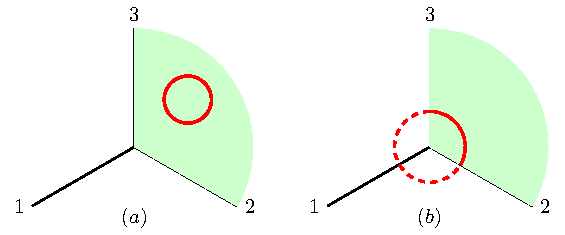
\includegraphics[width=0.9\textwidth]{C3orbits}
  \caption[Orbits in a system with $\Cn{3}$ symmetry.]{
    The two different kinds of \po s in a system with
    $\Cn{3}$ symmetry.
    The green region is the chosen fundamental domain.
    The red cycles are \po s.
  }
  \label{fig:C3orbits}
\end{figure}

$\Cn{3}$ has two subgroups $\{e\}$ and $\{e, \shift, \shift_2\}$, so there
are two types of \po s as shown in \reffig{fig:C3orbits}. A type-(a)
orbit has symmetry $\{e\}$, \ie, no symmetry, and it has two replicas by
rotation $\shift$  and $\shift_2$ respectively, which are not shown in
this figure. So the contribution from
a type-(a) orbit to the \dzeta\
% \refeq{eq:zeta}
is $(1-t_p)^3$.
The cubic order refers to the a fact that there are three sibling orbits together.
Also, since the entire orbit is in the fundamental domain, we have
\[
  1/\zeta_a = (1 - t_{\hat{p}})^3
  \,.
\]
The hat on $p$ means that $t_{\hat{p}}$ is evaluated only on the part of the orbit that
is in the fundamental domain.
A type-(b) orbit is invariant under $e$, $\shift$ and $\shift_2$.
This orbit has no siblings and only one third
of this orbit is in the fundamental domain. The other two thirds are replicas
by rotation $\shift$  and $\shift_2$ of the part in the fundamental domain. So, its
contribution to \dzeta\ is
\[
  1/\zeta_b = 1 - t_p = 1 - t_{\hat{p}}^3
  \,.
\]
Here, relation $t_p= t_{\hat{p}}^3$ is easily obtained by its definition in
\refeq{eq:zeta}.
On the other hand, by \refexam{exam:C3regularRep},
we know that the regular representations of $e$,
$\shift$, and $\shift_2$ are respectively
\[
  D^{reg}(e) = %&=&
  \begin{bmatrix}
    1 & & \\
    & 1 & \\
    & & 1 \\
  \end{bmatrix} \,,  \quad
  % \continue
  D^{reg}(\shift) = %&=&
  \begin{bmatrix}
    ~ & 1 & ~\\
    ~ & ~ & 1\\
    1 & ~ & ~ \\
  \end{bmatrix}\,,  \quad
  D^{reg}(\shift_2) =
  \begin{bmatrix}
    ~ & ~ & 1\\
    1 & ~ & ~\\
    ~ & 1 & ~ \\
  \end{bmatrix}
  \,.
\]
You can easily verify that
\[
 (1 - t_{\hat{p}})^3 = \det(1 - D^{reg}(e)t_{\hat{p}}) \,, \quad
 1 - t_{\hat{p}}^3 = \det(1 - D^{reg}(\shift)t_{\hat{p}}) =
 \det(1 - D^{reg}(\shift_2)t_{\hat{p}})\,.
\]
Therefore, you see that the contribution from \po s to the
\dzeta\ in a system with $\Cn{3}$
symmetry are related to the regular representation of $\Cn{3}$.

\begin{figure}[h]
  \centering
  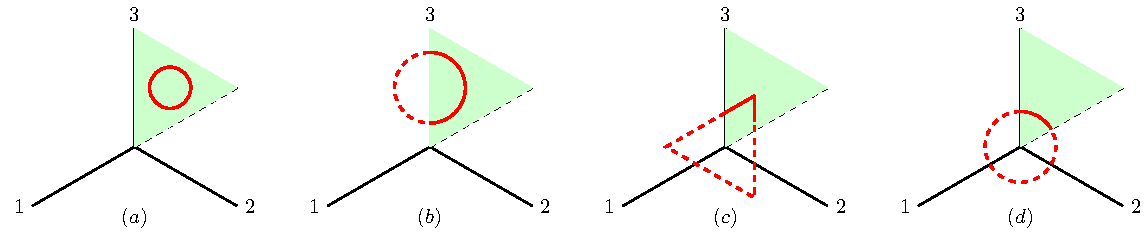
\includegraphics[width=0.9\textwidth]{D3orbits}
  \caption[Orbits in a system with $\Dn{3}$ symmetry.]{
    The four different kinds of \po s in a system with
    $\Dn{3}$ symmetry.
    The green region is the chosen fundamental domain.
    The red cycles are \po s.
  }
  \label{fig:D3orbits}
\end{figure}

Let us check out another example - a system with $\Dn{3}$ symmetry.
$\Dn{3}$ has four different kinds of subgroups $\{e\}$, $\{e, \Refl\}$,
$\{e, \shift, \shift_2\}$, and $\Dn{3}$ itself. Here $\Refl$ can be
any one of $\Refl_{12}$, $\Refl_{23}$ or $\Refl_{31}$. Accordingly,
there are four types of \po s as shown in \reffig{fig:D3orbits}.
The fundamental domain is one sixth of the full \statesp.
Similar to the analysis of the two orbits in the $\Cn{3}$ case, we have
\[
  1/\zeta_a = (1 - t_{\hat{p}})^6
  \,,\quad
  1/\zeta_b = (1 - t_{\hat{p}}^2)^3
  \,,\quad
  1/\zeta_c = (1 - t_{\hat{p}}^3)^2
  \,,\quad
  1/\zeta_d = 1 - t_{\hat{p}}^6
  \,.
\]
\refExam{exam:D3regularRep??} gives the regular representation of $\Dn{3}$.
You can also verify that
\begin{align*}
   & (1 - t_{\hat{p}})^6 = \det(1 - D^{reg}(e)t_{\hat{p}}) \,, \quad
     (1 - t_{\hat{p}}^2)^3 = \det(1 - D^{reg}(\Refl)t_{\hat{p}}) \\
   & (1 - t_{\hat{p}}^3)^2 = \det(1 - D^{reg}(\shift)t_{\hat{p}})\,,\quad
     1 - t_{\hat{p}}^6 = ?
     \,.
\end{align*}
I leave a question mark above since no analogous expression exists for it.
We will come back to it after proving
the identity \refeq{eq:symfac}.

We can generalize the above observation for a system invariant under
a general discrete group
$\Group=\{e, \LieEl_2, \LieEl_3,\cdots, \LieEl_{|\Group|}\}$.
Let $h$ be an element of $\Group$
with order (period) $m$, \ie, $m$ is the smallest positive integer such
that $h^m = e$. Then we have
\begin{equation}
  \label{eq:symfac}
  (1 - t^m)^{\frac{|G|}{m}} = \det(1 - D^{reg}(h)t)
  \,.
\end{equation}
The proof starts from the matrix identity $\ln\det = \tr\ln$, by which we have
\[
  \ln \det(1 - D^{reg}(h)t) = \tr \ln (1 - D^{reg}(h)t)
  = -\sum_{k=1}^\infty \frac{\tr D^{reg}(h^k)t^k}{k}
  \,.
\]
The last identity above comes from the Taylor expansion
$\ln(1-x) = -\sum_{k=1}^\infty \frac{x^k}{k}$.
As we know, the regular representation of
a group element has nonzero trace if and only if this group element is
$e$. So we have,
\[
  \ln \det(1 - D^{reg}(h)t) =  -\sum_{k=1}^\infty \frac{|G|t^{mk}}{mk}
  =  -\frac{|G|}{m}\sum_{k=1}^\infty \frac{t^{mk}}{k}
  = \frac{|G|}{m} \ln (1 - t^m)
  \,.
\]
Therefore, we obtain \refeq{eq:symfac}. This is why we have the observation
in the $\Cn{3}$ and $\Dn{3}$ example. However, for the type-(d) orbit in
\reffig{fig:D3orbits}, the symmetry group of this orbit is
$\{e, \Refl_{12}, \Refl_{32}, \Refl_{13}, \shift, \shift_2\}$. The order of
$\Refl$ is 2 while the order of $\shift$ is 3. The least common multiple is
6. Therefore, the contribution to the \dzeta\ is $(1-t_{\hat{p}}^6)^{1}$ and it
cannot be written as form $\det(1 - D^{reg}(h)t_{\hat{p}})$ with some $h\in G$.

Actually, we can write
\[
  1-t_{\hat{p}}^6 = \det(1 - D^{reg}(\shift)t_{\hat{p}}^2) \,,\quad
  \text{or} \quad
  1-t_{\hat{p}}^6 = \det(1 - D^{reg}(\Refl)t_{\hat{p}}^3)
\]
With $D^{reg}(\shift)$ the $[3\times 3]$ representation of $\shift$ in group $\Cn{3}$
and $ D^{reg}(\Refl)$ the $[2\times 2]$ representation of $\Refl$ in
reflection group $\{e, \Refl\}$. Anyway, for the type-(d) orbit we
have no choice but to give up the regular representation of $\Dn{3}$.

\subsection{Factorization of $C_n$ and $D_n$}

for a discrete symmetry group
$G=\{{ e},{ g}_2,\ldots,{ g}_{|G|}\}$. The orthogonality and completeness
of projection operator
can be easily verified by the orthogonality relation among characters of
irreducible representation. Define $ \cal L_\alpha=P_\alpha \cal L$, then
the trace of {\evOper} $\cal L$ can be decomposed into a sum of
$ \sum_\alpha \tr {\cal L}_\alpha$ because of the completeness of projection
operators.
\Xiong{2014-05-03}{Here the decomposition of trace just relies on the
  completeness of projection operators, we haven't used the commuting
  relation between {\evOper} and group transform. Am I right?}
So we only need to investigate the projected trace formula:
\begin{align*}
  \tr {\cal L}_\alpha & = \frac{d_\alpha}{|G|}\sum_{h \LieEl\in\Group} \chi_\alpha (h)
                        {\bf h}^{-1} \int_\pS dx \, {\cal L} ( x,x) \\
                      & =\frac{d_\alpha}{|G|}\sum_{h \LieEl\in\Group} \chi_\alpha (h) {\bf h}^{-1}
                        \sum_{a \LieEl\in\Group}\int_{\tilde{\pS}} d(a\tilde{x}) \,{\cal L} (a\tilde{x},a\tilde{x})
  \\
                      & =\frac{d_\alpha}{|G|}\sum_{h \LieEl\in\Group} \chi_\alpha (h) {\bf h}^{-1}\,\cdot
                        |G|\int_{\tilde{\pS}} d(\tilde{x}) \,{\cal L} (\tilde{x},\tilde{x}) \\
                      & = d_\alpha \sum_{h \LieEl\in\Group} \chi_\alpha (h) \int_{\tilde{\pS}} d\tilde{x} \,
                        {\cal L} ({\bf h}^{-1} \tilde{x},\tilde{x})
\end{align*}
In the above derivation, we have used the invariance of {\evOper}
under group transform. For a \po\ in the fundamental domain
$\tilde{p}$, we follow the standard argument in Chaosbook and get
\[
  \int_{\tilde{\pS}} d\tilde{x} \, {\cal L} ({\bf h}^{-1} \tilde{x},\tilde{x}) =
  \cl{\tilde{p}} \sum_{r=1}^\infty
    \frac{ e^{r \beta \cdot \Obser_{\tilde{p}}}}
         {|\det \left( {\bf 1}- {\tilde\monodromy}_{\tilde{p}}^r \right)|}
    \delta_{n,\cl{\tilde{p}} r}\delta_{h,h_{\tilde{p}}^r}
  \,;
\]
so, the {\Fd} is
\bea
F(z) &=& \prod_\alpha F_\alpha (z)^{d_\alpha}
\continue   %\,\, , \quad \quad
F_\alpha (z) &=&
{\rm exp}  \left( - {
    \sum_{\tilde{p}} \sum_{r=1}^\infty \frac{1}{r}
    \frac{\chi_\alpha (h_{\tilde{p}}^r)  z^{\cl{\tilde{p}} r}
          e^{r \beta \cdot \Obser_{\tilde{p}}}}
         {|\det \left( {\bf 1}- {\tilde\monodromy}_{\tilde{p}}^r \right)|}
  } \right)
\,\,  ,
\eea
which is discrete factorization for maps. The same method can be applied to
flows with discrete symmetry:
\[
  F_\alpha (z) =
  {\rm exp}  \left( - {
      \sum_{\tilde{p}} \sum_{r=1}^\infty \frac{1}{r}
      \frac{\chi_\alpha (h_{\tilde{p}}^r) e^{r (\beta \cdot \Obser_{\tilde{p}}-sT_{\tilde{p}})}
      }{| \det \left( {\bf 1}- {\tilde\monodromy}_{\tilde{p}}^r \right) | }
    } \right)
\]

Making an approximation
$| \det \left( {\bf 1}- {\tilde\monodromy}_{\tilde{p}}^r \right) | \approx
|\Lambda_{\tilde{p}}|$ where $\Lambda_{\tilde{p}}$ is the product of all
expanding multipliers, we get the factorized zeta function:
\begin{equation}
  F_\alpha (z) =
  {\rm exp}  \left( -
    \sum_{\tilde{p}} \sum_{r=1}^\infty \frac{1}{r}
    \chi_\alpha (h_{\tilde{p}}^r) t_{\tilde{p}}^r \right)
  \label{eq:redzeta}
\end{equation}

Formula \eqref{eq:redzeta} is the ultimate goal of Discrete Factorization,
which basically tells us that,
equipped with character table of the group in question, we can write down
all the factorized zeta function for all classes of this group. On the
other hand, in order to verify our result,
let's calculate the zeta
function in the full \statesp.
\begin{align*}
  F(z) &= \prod_\alpha F_\alpha (z)^{d_\alpha} \\
       &= {\rm exp}  \left( -
         \sum_{\tilde{p}} \sum_{r=1}^\infty \frac{1}{r}\sum_{\alpha}
         \left(d_{\alpha}\chi_\alpha (h_{\tilde{p}}^r)\right) t_{\tilde{p}}^r \right) \\
       &= {\rm exp}  \left( -
         \sum_{\tilde{p}} \sum_{r=1}^\infty \frac{1}{r}
         |G|\delta_{h_{\tilde{p}}^r}  t_{\tilde{p}}^r \right) \\
       &= {\rm exp}  \left( -
         \sum_{\tilde{p}} \sum_{k=1}^\infty \frac{|G|}{mk}
         t_{\tilde{p}}^{mk} \right)
         \,,
\end{align*}
that is
\begin{equation}
  \label{eq:fullzeta}
  F(z)= \left(1-t_{\tilde{p}}^{\frac{|G|}{m}}\right)^{m} \,,
\end{equation}
where $m$ is the smallest positive number such that $h_{\tilde{p}}^{m}=e$, namely
the multiplicity of the \po\ in the full \statesp.
Formula \eqref{eq:fullzeta} is just the left side of
\beq
(1-t_{\tilde{p}}^{h_p})^{g/h_p}
=\det \left(1- D(h_{\tilde p}) t_{\tilde p} \right)
=
\prod_{\alpha} \det(1-D_{\alpha}(h_{\tilde{p}}) t_{\tilde{p}} )^{d_\alpha}
\eeq
in Chaosbook and actually formula \eqref{eq:redzeta} is the right side of
it. For completeness, I derive their equivalence here. By the
definition of character and representation of a group,
$\chi_\alpha (h_{\tilde{p}}^r)= \tr D_{\alpha}(h_{\tilde{p}}^r)
=\tr (D_{\alpha}(h_{\tilde{p}}))^r$ where $D$ is the regular representation
of this group, so \eqref{eq:redzeta} can be rewritten as follows,
\begin{align*}
  F_\alpha (z) & =
                 {\rm exp}  \left( -
                 \tr \sum_{\tilde{p}} \sum_{r=1}^\infty \frac{1}{r}
                 (D_{\alpha}(h_{\tilde{p}}))^r t_{\tilde{p}}^r \right) \\
               & ={\rm exp}  \left(
                 \tr \sum_{\tilde{p}} \ln (1-D_{\alpha}(h_{\tilde{p}}))
                 \right) \\
               & = \prod_{\tilde{p}} \det(1-D_{\alpha}(h_{\tilde{p}}))
\end{align*}
Here, we have used relation $\tr \ln= \ln \det$. All calculation of
factorized zeta function in Chaosbook is conducted by
$\det(1-D_{\alpha}(h_{\tilde{p}}))$, but I are apt to use \eqref{eq:redzeta}
because it doesn't contain information about any specific representation.
\Xiong{2014-05-05}{I am not sure whether I understand it correctly here.}
All the following examples are analyzed by \eqref{eq:redzeta}.

\paragraph{$C_{n}$} case

When $h_{\tilde p}=e$,
\[
  F_{A}=F_{\Gamma_j}={\rm exp} (-\sum_{r=1}^\infty \frac{1}{r}t_{\tilde{p}}^r )
  =1-t_{\tilde p}
  \,,
\]
Where we only investigate the contribution from one specific periodic
orbit and ignore the summation $ \sum_{\tilde{p}}$.

When $h_{\tilde p}=C_n^k$, Similarly,
\[
  F_{A}=1-t_{\tilde p}
\]
\[
  F_{\Gamma_j}={\rm exp} (-\sum_{r=1}^\infty \frac{1}{r}e^{\frac{i2\pi kjr}{n}}
  t_{\tilde{p}}^r )
  =1-e^{\frac{i2\pi kj}{n}} t_{\tilde p}
  \,,
\]
In sum,
\vskip 12pt
\begin{tabular}{rlccc}

  $h_{\tilde p}$ &  & &  $A$  &  $\Gamma_{j}$ \\
  $e$:
                 & $(1-t_{\tilde p} )^n$  &=&$(1-t_{\tilde p})$ & $(1-t_{\tilde p})$  \\
  $C_n^{k}$:
                 & $(1-t_{\tilde p}^m )^{\frac{n}{n}}$ &=&  $(1-t_{\tilde p})$ & $(1-\exp(\frac{i2\pi kj}{n})t_{\tilde p})$ \\
\end{tabular}
\vskip 12pt
\noindent


\paragraph{$D_{n}$ ($n$ odd)} case:
When $h_{\tilde p}=e$,
\[
  F_{A_1}=F_{A_2}={\rm exp} (-\sum_{r=1}^\infty \frac{1}{r}t_{\tilde{p}}^r )
  =1-t_{\tilde p}
\]
\[
  F_{E_j}={\rm exp} (-\sum_{r=1}^\infty \frac{2}{r}t_{\tilde{p}}^r )
  =(1-t_{\tilde p})^2
\]
When $h_{\tilde p}=C_n^k$, the same goes for $A_1$ and $A_2$:
$F_{A_1}=F_{A_2}=1-t_{\tilde p}$, but for $E_j$, it requires a little
special treatment.
\begin{align*}
  F_{E_j}= & {\rm exp} (-\sum_{r=1}^\infty \frac{1}{r}2\cos\frac{2\pi kjr}{n}
             t_{\tilde{p}}^r ) \\
  = & {\rm exp} \left(-\sum_{r=1}^\infty \frac{1}{r}(\exp(\frac{i2\pi
      kjr}{n})+\exp(-\frac{i2\pi kjr}{n}))t_{\tilde{p}}^r \right) \\
  = & \left(1-\exp(\frac{i2\pi kj}{n})t_{\tilde p} \right)
      \left(1-\exp(-\frac{i2\pi kj}{n})t_{\tilde p} \right) \\
  = & 1-2\cos\frac{2\pi kj}{n}t_{\tilde p}+t_{\tilde p}^2
\end{align*}
When $h_{\tilde p}\in \{\Refl,\Refl_{1},\cdots,\Refl_{n-1}\}$,
$h_{\tilde p}^2=e$.
\begin{align*}
  F_{A_1}= &1-t_{\tilde p} \\
  F_{A_2}= &{\rm exp} (-\sum_{r=even}^\infty \frac{1}{r}t_{\tilde{p}}^r
             +\sum_{r=odd}^\infty \frac{1}{r}t_{\tilde{p}}^r )
             =(1+t_{\tilde p}) \\
  F_{E_j}= &{\rm exp} (-\sum_{r=even}^\infty \frac{1}{r}2t_{\tilde{p}}^r)
             =(1-t_{\tilde p}^2)
\end{align*}

In sum,

\vskip 12pt
\begin{tabular}{rlcccc}

  $h_{\tilde p}$ &  & &  $A_1$  &  $A_2$  &  $E_j$  \\
  $e$:
                 & $(1-t_{\tilde p} )^{2n}$  &=&$(1-t_{\tilde p})$ & $(1-t_{\tilde p})$ &
                                                                                          $ (1-t_{\tilde p})^4 $ \\
  $C_n^k,C_n^{n-k} $:
                 & $(1-t_{\tilde p}^m )^{\frac{2n}{m}}$ &=&  $(1-t_{\tilde p})$ & $(1-t_{\tilde p})$ &
                                                                                                       $ (1-2\cos(\frac{2\pi kj}{n})t_{\tilde p}+t^{2}_{\tilde p})^2 $ \\
  $\Refl,\Refl_{1},\cdots,\Refl_{n-1}$:
                 & $(1-t_{\tilde p}^2 )^{n}$ &=&  $(1-t_{\tilde p})$ &                      $(1+t_{\tilde p})$ &$ (1-t_{\tilde p}^2)^2 $ \\
\end{tabular}
\vskip 12pt
\noindent


\paragraph{$\Dn{n}$ ($n$ even)} case:
% When $h_{\tilde p}=e$, we have $F_{A_1}= %F_{A_2}=F_{B_1}=F_{B_2}=1-t_{\tilde p}$
% and $F_{E_j}=(1-t_{\tilde p})^2$
%
% When $h_{\tilde p}=C_2$, similarly, $F_{A_1}= F_{A_2}=1-t_{\tilde p}$,
% $F_{B_1}=F_{B_2}=1-(-1)^{n/2}t_{\tilde p}$ and
% $F_{E_j}=(1-(-1)^jt_{\tilde p})^2$.

Similar calculation gives us the following
factorized zeta function table.

\vskip 12pt
\begin{center}
  \begin{tabular}{b{1cm}lcccccl}

    $h_{\tilde p}$ &  & &  $A_1$  &  $A_2$  &  $B_1$  &  $B_2$  &  $E_{j}$  \\
    $e$:
                   & $(1-t_{\tilde p} )^{2n}$  &=&$(1-t_{\tilde p})$ & $(1-t_{\tilde p})$ &
                                                                                            $(1-t_{\tilde p})$ &$(1-t_{\tilde p})$&$ (1-t_{\tilde
                                                                                                                                    p})^4 $ \\
    $\shift_{n/2}$:
                   & $(1-t_{\tilde p}^2 )^n$ &=&  $(1-t_{\tilde p})$ & $(1-t_{\tilde p})$ &
                                                                                            $(1-(-1)^{\frac{n}{2}}t_{\tilde p})$ &$(1-(-1)^{\frac{n}{2}}t_{\tilde p})$ &
                                                                                                                                                                         $(1-(-1)^jt_{\tilde p})^4 $ \\
    $\shift_{k}$ (odd):
                   & $(1-t_{\tilde p}^m )^{\frac{2n}{m}}$ &=&  $(1-t_{\tilde p})$ & $(1-t_{\tilde p})$ &
                                                                                                         $(1+t_{\tilde p})$ &$(1+t_{\tilde p})$ &
                                                                                                                                                  $ (1-2\cos(\frac{2\pi kj}{n})t_{\tilde p}+t^{2}_{\tilde p})^2 $ \\
    $\shift_{k}$ (even):
                   & $(1-t_{\tilde p}^m )^{\frac{2n}{m}}$ &=&  $(1-t_{\tilde p})$ & $(1-t_{\tilde p})$ &
                                                                                                         $(1-t_{\tilde p})$ &$(1-t_{\tilde p})$ &
                                                                                                                                                  $ (1-2\cos(\frac{2\pi kj}{n})t_{\tilde p}+t^{2}_{\tilde p})^2 $ \\
    $\Refl$:
                   & $(1-t_{\tilde p}^2 )^n$&=& $(1-t_{\tilde p})$ & $(1+t_{\tilde p})$ &
                                                                                          $(1-t_{\tilde p})$ &$(1+t_{\tilde p})$& $ (1-t_{\tilde p}^2)^2 $ \\
    $\shift\Refl$:
                   & $(1-t_{\tilde p}^2 )^n$&=& $(1-t_{\tilde p})$ & $(1+t_{\tilde p})$ &
                                                                                          $(1+t_{\tilde p})$ &$(1-t_{\tilde p})$& $ (1-t_{\tilde p}^2)^2 $ \\
  \end{tabular}
\end{center}
\vskip 12pt
\noindent

When it comes to continuous symmetry, projection operator is
\beq
{P}_\eigenvG
= d_\eigenvG \int_{G} dg\,
\, \chi_\eigenvG(g^{-1})  O_g
\,.
\eeq
The corresponding trace formula in the irreducible subspace is
\beq
\sum_{\beta=0}^\infty
    \frac{1}{\eigenvL -\eigenvL_{\eigenvG,\beta} }
=
d_\eigenvG \sum_p
\period{p}
\sum_{r=1}^\infty
\chi_\eigenvG( g_p^r)
\frac{e^{r (\beta \Obser_p -\eigenvL\period{p})}}
     {{\left|\det\!\left(\matId-
        \tilde{\monodromy}_{\eigenvG,p}^r\right)\right|}}
\,.
\eeq
Therefore the \Fd\ is factorized as

\bea
\det(\eigenvL - \Aop) &=& \prod_\alpha F_\alpha (z)^{d_\alpha}
\continue   %\,\, , \quad \quad
F_\alpha (z) &=&
{\rm exp}  \left(
    - {
    \sum_{\tilde{p}} \sum_{r=1}^\infty \frac{1}{r}
    \frac{\chi_\alpha (g_{\tilde{p}}^r)  z^{\cl{\tilde{p}} r}
      e^{r \beta \cdot \Obser_{\tilde{p}}}
      % {\phi_p^r}
      } {| \det \left( {\bf 1}- {\tilde\monodromy}_{\tilde{p}}^r \right) | }
       } \right)
\,\,
\eea
It differs from the discrete case on that now the group operator
$g_{\tilde{p}}$ is continuous and the factorization may have infinite terms.

\paragraph{Used formulas} Here I list several formulas used in the
above post.

\begin{equation}
  \frac{1}{2\pi}\sum_{n=-\infty}^{\infty}e^{inx} = \delta(x)
\end{equation}
This identity comes from one definition of delta function
$\delta(x)=\lim_{N\to \infty}
\frac{1}{2\pi}\frac{\sin(N+1/2)x}{\sin(\frac{1}{2}x)}$ and simple
calculation gives
$\sum_{n=-N}^{N}e^{inx}=\frac{\sin(N+1/2)x}{\sin(\frac{1}{2}x)}$.

\begin{equation}
  \sum_{R}\chi_\alpha(R) \chi_\beta(SR^{-1})=\frac{|G|}{d_\alpha}\,
  \delta _{\alpha,\beta} \chi_\alpha(S)
\end{equation}
This is the orthogonality between characters of irreducible
representations. If we set $S=e$, then it reduces to
$\sum_{R}\chi_\alpha(R) \chi_\beta(R^{-1})=|G|\delta _{\alpha,\beta}$.
The orthogonality of projection operators can be checked:
\begin{align*}
  P_\alpha P_\beta = & \frac{d_\alpha}{|G|}\, \frac{d_\beta}{|G|}
                       \sum_{h,s\LieEl\in\Group} \chi_\alpha (h) \chi_\alpha (s) {\bf h}^{-1} {\bf s}^{-1} \\
  = & \frac{d_\alpha}{|G|}\, \frac{d_\beta}{|G|} \sum_{s\LieEl\in\Group}
      \frac{|G|}{d_\alpha}\,\delta _{\alpha,\beta} \chi_\alpha(sh)(\bf{sh})^{-1} \\
  = &\delta _{\alpha,\beta} \frac{d_\alpha}{|G|}\,\sum_{s\LieEl\in\Group}
      \chi_\alpha(s){\bf s}^{-1} \\
  = & \delta _{\alpha,\beta}\, P_\alpha
\end{align*}

The last formula is
\begin{equation}
  \sum_\alpha d_\alpha \chi_\alpha (R) = |G|\, \delta_{e,R}
  \label{eq:groupcomplete}
\end{equation}
which comes from orthogonality relation above. For regular representation,
the trace of $R$ in terms of irreducible representations is
$\chi (R)=\sum_\alpha a_\alpha \chi_\alpha (R)$, so the summation of all group
elements gives
\[
  \sum_{R}\chi (R)\chi_\alpha (R^{-1})=\sum_\alpha a_\alpha \sum_{R}
  \chi_\alpha (R) \chi_\alpha (R^{-1}) =|G|\, a_\alpha
\]
On the other hand, $\chi (R)=|G|\, \delta_{e,R}$ for regular representation,
then the left side of the above expression is just $|G|\,\chi_\alpha (e)$,
so $a_\alpha =\chi_\alpha (e) =d_\alpha $ the dimension of $\alpha_{th}$
irreducible representation. In this way, we obtain \refeq{eq:groupcomplete}.
Now the completeness of projection operator can be checked:
\[
  \sum_\alpha P_\alpha = \sum_\alpha \frac{d_\alpha}{|G|} \sum_{h\LieEl\in\Group}
  \chi_\alpha (h)  {\bf h}^{-1}
  =\frac{1}{|G|} \sum_{h\LieEl\in\Group} \left(\sum_\alpha d_\alpha \chi_\alpha (h)
  \right){\bf h}^{-1}
  =e
\]



\renewcommand{\Refl}{\ensuremath{\sigma}}             % in DasBuch
\renewcommand{\shift}{\ensuremath{d}}                 % in DasBuch
\renewcommand{\ssp}{x}
\renewcommand{\Xx}{\ensuremath{\mathsf{X}}}      % Boris
\renewcommand{\Ssym}[1]{{\ensuremath{s_{#1}}}}  % ChaosBook

%%%%%%%%%%%%%%%%%%%%%%%%%%%%%%%%%%%%%%%%%%%%%%%%
\printbibliography[heading=subbibintoc,title={References}]
